%Este trabalho está licenciado sob a Licença Creative Commons Atribuição-CompartilhaIgual 3.0 Não Adaptada. Para ver uma cópia desta licença, visite http://creativecommons.org/licenses/by-sa/3.0/ ou envie uma carta para Creative Commons, PO Box 1866, Mountain View, CA 94042, USA.

%%%%%%%%%%%%%%%%%%%%%%%%%%%%%%%%%%%%%%%%%%
% ATENÇÃO
%
% POR SEGURANÇA, NÃO EDITE ESTE ARQUIVO
%
%%%%%%%%%%%%%%%%%%%%%%%%%%%%%%%%%%%%%%%%%

\documentclass[12pt]{book}

\input preambulo.tex

\begin{document}

\frontmatter

%titlepage
\title{Cálculo Numérico\\\small{Um Livro Colaborativo}}
\author{}
\date{\today}
\addcontentsline{toc}{chapter}{Capa}

\ifishtml
\else
\AddToShipoutPicture*{\BackgroundPic}
\fi
\maketitle

%Este trabalho está licenciado sob a Licença Creative Commons Atribuição-CompartilhaIgual 3.0 Não Adaptada. Para ver uma cópia desta licença, visite http://creativecommons.org/licenses/by-sa/3.0/ ou envie uma carta para Creative Commons, PO Box 1866, Mountain View, CA 94042, USA.

\chapter*{Organizadores}
\addcontentsline{toc}{chapter}{Organizadores}

\begin{itemize}
\item[] Dagoberto Adriano Rizzotto Justo - UFRGS
\item[] Esequia Sauter - UFRGS
\item[] Fabio Souto de Azevedo - UFRGS
\item[] Leonardo Fernandes Guidi - UFRGS
\item[] Matheus Correia dos Santos - UFRGS
\item[] Pedro Henrique de Almeida Konzen - UFRGS
\end{itemize}
%Este trabalho está licenciado sob a Licença Creative Commons Atribuição-CompartilhaIgual 3.0 Não Adaptada. Para ver uma cópia desta licença, visite https://creativecommons.org/licenses/by-sa/3.0/ ou envie uma carta para Creative Commons, PO Box 1866, Mountain View, CA 94042, USA.

\chapter*{Licença}
\addcontentsline{toc}{chapter}{Licença}

Este trabalho está licenciado sob a Licença Creative Commons Atribuição-CompartilhaIgual 3.0 Não Adaptada. Para ver uma cópia desta licença, visite https://creativecommons.org/licenses/by-sa/3.0/ ou envie uma carta para Creative Commons, PO Box 1866, Mountain View, CA 94042, USA.

%Este trabalho está licenciado sob a Licença Creative Commons Atribuição-CompartilhaIgual 3.0 Não Adaptada. Para ver uma cópia desta licença, visite http://creativecommons.org/licenses/by-sa/3.0/ ou envie uma carta para Creative Commons, PO Box 1866, Mountain View, CA 94042, USA.

\chapter*{Nota dos organizadores}
\addcontentsline{toc}{chapter}{Nota dos organizadores}

Este livro vem sendo construído de forma colaborativa desde 2011. Nosso intuito é melhorá-lo, expandi-lo e adaptá-lo às necessidades de um curso de cálculo numérico em nível de graduação.

Caso queira colaborar, tenha encontrado erros, tenha sugestões ou reclamações, entre em contato conosco pela lista de emails:
\begin{center}
\url{livro_colaborativo@googlegroups.com}  
\end{center}
Alternativamente, abra um chamado no repositório GitHub do projeto:
\begin{center}
\url{https://github.com/livroscolaborativos/CalculoNumerico}  
\end{center}
ou, ainda, envie um email para:
\begin{center}
\url{livroscolaborativos@gmail.com}
\end{center}

Mais informações também estão disponíveis no página oficial do projeto:
\begin{center}
\url{http://www.ufrgs.br/numerico}  
\end{center}



%Este trabalho está licenciado sob a Licença Creative Commons Atribuição-CompartilhaIgual 3.0 Não Adaptada. Para ver uma cópia desta licença, visite http://creativecommons.org/licenses/by-sa/3.0/ ou envie uma carta para Creative Commons, PO Box 1866, Mountain View, CA 94042, USA.

\chapter*{Prefácio}
\addcontentsline{toc}{chapter}{Prefácio}

Este livro busca abordar os tópicos de um curso de introdução ao cálculo numérico moderno oferecido a estudantes de matemática, física, engenharias e outros. A ênfase é colocada na formulação de problemas, implementação em computador da resolução e interpretação de resultados. Pressupõe-se que o estudante domine conhecimentos e habilidades típicas desenvolvidas em cursos de graduação de cálculo, álgebra linear e equações diferenciais. Conhecimentos prévios em linguagem de computadores é fortemente recomendável, embora apenas técnicas elementares de programação sejam realmente necessárias.

\ifisscilab
Ao longo do livro, fazemos ênfase na utilização do \emph{software} livre \verb+Scilab+ para a implementação dos métodos numéricos abordados. Recomendamos que o leitor ter à sua disposição um computador com o \verb+Scilab+ instalado. Não é necessário estar familiarizado com a linguagem \verb+Scilab+, mas recomendamos a leitura do Apêndice~\ref{cap:scilab}, no qual apresentamos uma rápida introdução a este pacote computacional. Alternativamente, existem algumas soluções em nuvem que fornecem acesso ao Scilab via internet. Por exemplo, a plataforma virtual rollApp (\url{https://www.rollapp.com/app/scilab}).
\fi



\ifisslide
\tableofcontents
\else
\tableofcontents
\addcontentsline{toc}{chapter}{Sumário}
\fi

\mainmatter

%Este trabalho está licenciado sob a Licença Creative Commons Atribuição-CompartilhaIgual 3.0 Não Adaptada. Para ver uma cópia desta licença, visite http://creativecommons.org/licenses/by-sa/3.0/ ou envie uma carta para Creative Commons, PO Box 1866, Mountain View, CA 94042, USA.

\documentclass[main.tex]{subfiles}
\begin{document}
\chapter{Introdução}

Cálculo numérico é a disciplina que estuda as técnicas para a solução aproximada de problemas matemáticos. Estas técnicas são de natureza analítica e computacional. As principais preocupações normalmente envolvem exatidão e perfórmance. 

Aliado ao aumento contínuo da capacidade de computação disponível, o desenvolvimento de métodos numéricos tornou a simulação computacional\index{simulação!computacional} de modelos matemáticos uma prática usual nas mais diversas áreas científicas e tecnológicas. As então chamadas simulações numéricas\index{simulação!numérica} são constituídas de um arranjo de vários esquemas numéricos dedicados a resolver problemas específicos como, por exemplo: resolver equações algébricas, resolver sistemas lineares, interpolar e ajustar pontos, calcular derivadas e integrais, resolver equações diferenciais ordinárias, etc.. Neste livro, abordamos o desenvolvimento, a implementação, utilização e aspectos teóricos de métodos numéricos para a resolução desses problemas.

Os problemas que discutiremos não formam apenas um conjunto de métodos fundamentais, mas são, também, problemas de interesse na engenharia e na matemática aplicada. A necessidade de aplicar aproximações numéricas decorre do fato de que esses problemas podem se mostrar intratáveis se dispomos apenas de meios puramente analíticos, como aqueles estudados nos cursos de cálculo e álgebra linear. Por exemplo, o teorema de Abel-Ruffini nos garante que não existe uma fórmula algébrica, isto é, envolvendo apenas operações aritméticas e radicais, para calcular as raízes de uma equação polinomial de qualquer grau, mas apenas casos particulares:
\begin{itemize}
\item Simplesmente isolar a incógnita para encontrar a raiz de uma equação do primeiro grau;
\item Fórmula de Bhaskara para encontrar raízes de uma equação do segundo grau;
\item Fórmula de Cardano para encontrar raízes de uma equação do terceiro grau;
\item Existe expressão para equações de quarto grau;
\item Casos simplificados de equações de grau maior que 4 onde alguns coeficientes são nulos também podem ser resolvidos.
\end{itemize}
Equações não polinomiais podem ser ainda mais complicadas de resolver exatamente, por exemplo:
$$
\cos(x)=x\qquad \hbox{e}\qquad xe^x= 10
$$

Para resolver o problema de valor inicial 
$$
\begin{array}{l}
y'+xy=x,\\
y(0)=2,
\end{array}
$$
podemos usar o método de fator integrante e obtemos $y=1+e^{-x^2/2}$. Já o cálculo da solução exata para o problema 
$$
\begin{array}{l}
y'+xy=e^{-y},\\
y(0)=2,
\end{array}
$$
não é possível.

Da mesma forma, resolvemos a integral
$$
\int_1^2xe^{-x^2}dx
$$
pelo método da substituição e obtemos $\frac{1}{2}(e^{-1}-e^{-2})$. Porém a integral
$$
\int_1^2 e^{-x^2} dx
$$
não pode ser resolvida analiticamente.

A maioria dos modelos de fenômenos reais chegam em problemas matemáticos onde a solução analítica é difícil (ou impossível) de ser encontrada, mesmo quando provamos que ela existe. Nesse curso propomos calcular aproximações numéricas para esses problemas, que apesar de, em geral, serem diferentes da solução exata, mostraremos que elas podem ser bem próximas.

Para entender a construção de aproximações é necessário estudar um pouco como funciona a aritmética de computador e erros de arredondamento. Como computadores, em geral, usam uma base binária para representar números, começaremos falando em mudança de base.
\end{document}
%Este trabalho está licenciado sob a Licença Creative Commons Atribuição-CompartilhaIgual 3.0 Não Adaptada. Para ver uma cópia desta licença, visite http://creativecommons.org/licenses/by-sa/3.0/ ou envie uma carta para Creative Commons, PO Box 1866, Mountain View, CA 94042, USA.

%\documentclass[main.tex]{subfiles}
%\begin{document}

\chapter{Representação de números e aritmética de máquina}\index{representação de números}\index{aritmética!de máquina}

Neste capítulo, discutiremos sobre formas de representação de números em computadores. Iniciamos com uma discussão sobre representação posicional e mudança de base. Então, discutimos sobre representação com número de dígitos finitos e, mais especificamente, as representações de números inteiros, ponto fixo e ponto flutuante em computadores.

A representação de números e a aritmética em computadores levam aos chamados erros de arredondamento e de truncamento. Ao final deste capítulo, discutiremos sobre os efeitos do erro de arredondamento na computação científica.

%%%%%%%%%%%%%%%%%%%%
% python
%%%%%%%%%%%%%%%%%%%%
\ifispython
Ao longo do capítulo, faremos alguns comentários usando códigos em \verb+Python 2.7+. Nestes, estaremos assumindo que os seguintes módulos estão carregados:
\begin{verbatim}
>>> from __future__ import division
>>> import numpy as np
\end{verbatim}
A primeira instrução garante que divisões de números inteiros sejam computadas em ponto flutuante (\verb+double+) e a segunda carrega a biblioteca de computação científica \href{http://www.numpy.org/}{numpy}.
\fi

\section{Sistema de numeração e mudança de base}\index{mudança de base}\index{sistema de numeração}
Usualmente, utilizamos o sistema de numeração decimal para representar números. Esse é um sistema de numeração posicional onde a posição do dígito indica a potência de $10$ que o dígito está representando.

\begin{ex}
  O número $293$ é decomposto como
  \begin{equation*}
    \begin{split}
      293 &= 2\ \text{centenas}+9\ \text{dezenas}+3\ \text{unidades}\\
      &= 2\times 10^2+9\times 10^1+3\times 10^0.      
    \end{split}
  \end{equation*}
\end{ex}

O sistema de numeração posicional também pode ser usado com outras bases. Vejamos a seguinte definição.

\begin{defn}[Sistema de numeração de base $b$]\label{def:sistema_de_numeracao}
Dado um número natural $b>1$ e o conjunto de símbolos $\{\pmb{,}, \pmb{-},  \pmb{0}, \pmb{1}, \pmb{2},\dotsc, \pmb{b-1}\}$\footnote{Para $b>10$, veja a observação \ref{obs:sistema_de_numeracao}}, a sequência de símbolos
\begin{equation*}
  \left(d_nd_{n-1} \cdots d_1d_0,d_{-1}d_{-2} \cdots \right)_b  
\end{equation*}
representa o número positivo
\begin{equation*}
  d_n\cdot b^n + d_{n-1}\cdot b^{n-1} + \cdots + d_0\cdot b^0 + d_{-1}\cdot b^{-1}+d_{-2}\cdot b^{-2} + \cdots
\end{equation*}
Para representar números negativos usamos o símbolo $-$ a esquerda do numeral.
\end{defn}

\begin{obs}[$b\geq 10$]\label{obs:sistema_de_numeracao}
Para sistemas de numeração com base $b \geq 10$ é usual utilizar as seguintes notações:
\begin{itemize}
\item No sistema de numeração decimal ($b=10$), costumamos representar o número sem os parênteses e o subíndice, ou seja,
\begin{equation*}
  \pm d_nd_{n-1}\ldots d_1d_0,d_{-1}d_{-2}\ldots := \pm (d_nd_{n-1}\ldots d_1d_0,d_{-1}d_{-2}\ldots)_{10}  
\end{equation*}
\item Se $b>10$, usamos as letras $A, B, C, \cdots$ para completar os símbolos: $A=10$, $B=11$, $C=12$, $D=13$, $E=14$, $F=15$.
\end{itemize}
\end{obs}


\begin{ex}[Sistema binário] O sistema de numeração em base dois é chamado de binário e os algarismos binários são conhecidos como \textit{bits}, do inglês \textit{\bf{b}inary dig\bf{its}}. Um \textit{bit} pode assumir dois valores distintos: $0$ ou $1$. Por exemplo:
\begin{equation*}
  \begin{split}
    x &= (1001,101)_{2} \\
    &= 1\cdot 2^3 +0\cdot 2^2 +0\cdot 2^1 +1\cdot 2^0  +1\cdot 2^{-1} +0\cdot 2^{-2} +1\cdot 2^{-3} \\
    &= 8+0+0+1+ 0,5+0+0,125 = 9,625    
  \end{split}
\end{equation*}
Ou seja, $(1001,101)_{2}$ é igual a $9,625$ no sistema decimal.
\end{ex}


\begin{ex}[Sistema quaternário]
No sistema quaternário a base $b$ é igual a $4$. Por exemplo:
  \begin{equation*}
    (301,2)_{4}=3\cdot 4^2+0\cdot 4^1+1\cdot 4^0+2\cdot 4^{-1}=49,5    
  \end{equation*}
\end{ex}

\begin{ex}[Sistema octal]
No sistema octal a base é $b=8$ e utilizamos os símbolos em $\{0, 1, 2, 3, 4, 5, 6, 7\}$. Por exemplo:
\begin{equation*}
  \begin{split}
    (1357,24)_{8}&= 1\cdot 8^3+3\cdot 8^2+5\cdot 8^1+7\cdot 8^{0}+2\cdot 8^{-1}+4\cdot 8^{-2}\\
    &= 512+192+40+7+0,25+0,0625=751,3125    
  \end{split}
\end{equation*}
\end{ex}

\begin{ex}[Sistema hexadecimal] O sistema de numeração cuja a base é $b=16$ é chamado de sistema hexadecimal. O conjunto de símbolos necessários é  $S=\{``,", -, 0, 1, 2, 3, 4, 5, 6, 7, 8, 9, A, B, C, D, E, F\}$. Convertendo o número $(E2AC)_{16}$ para a base $10$ temos
\begin{equation*}
  \begin{split}
  (E2AC)_{16} &= 14\cdot 16^3+2\cdot 16^2+10\cdot 16^1+12\cdot 16^{0}\\
  &=57344+512+160+12=58028  
  \end{split}
\end{equation*}
\end{ex}

%%%%%%%%%%%%%%%%%%%%
% scilab
%%%%%%%%%%%%%%%%%%%%
\ifisscilab
\begin{obs}
  O \verb+Scilab+ oferece algumas funções para a conversão de números inteiros em dada base para a base decimal. Por exemplo, temos:
\begin{verbatim}
-->bin2dec('1001')
 ans  =
    9.  
-->hex2dec('451')
 ans  =
    1105.  
-->oct2dec('157')
 ans  =
    111.
-->base2dec('BEBA',16)
 ans  =
    48826.  
\end{verbatim}
\end{obs}
\fi
%%%%%%%%%%%%%%%%%%%%
%%%%%%%%%%%%%%%%%%%%
% octave
%%%%%%%%%%%%%%%%%%%%
\ifisoctave
\begin{obs}
  O \verb+GNU Octave+ oferece algumas funções para a conversão de números inteiros em dada base para a base decimal. Por exemplo, temos:
\begin{verbatim}
>> bin2dec('1001')
ans =  9
>> hex2dec('451')
ans =  1105
>> base2dec('157',8) #oct -> dec
ans =  111
>> base2dec('BEBA',16)
ans =  48826
\end{verbatim}
\end{obs}
\fi
%%%%%%%%%%%%%%%%%%%%
%%%%%%%%%%%%%%%%%%%%
% python
%%%%%%%%%%%%%%%%%%%%
\ifispython
\begin{obs}
  \verb+Python+ tem algumas sintaxes para representar números em algumas bases. Por exemplo, temos:
\begin{verbatim}
>>> print(0b1001) #bin -> dec
9
>>> print(0157) #oct -> dec
111
>>> print(0xbeba) #hex -> dec
48826
\end{verbatim}
\end{obs}
\fi
%%%%%%%%%%%%%%%%%%%%

A partir da definição \ref{def:sistema_de_numeracao}, acabamos de mostrar vários exemplos de conversão de números de uma sistema de numeração de base $b$ para o sistema decimal. Agora, vamos estudar como fazer o processo inverso. Isto é, dado um número decimal $(X)_{10}$ queremos escrevê-lo em uma outra base $b$, isto é, queremos obter a seguinte representação:
\begin{equation*}
  \begin{split}
    (X)_{10} &= (d_nd_{n-1}\cdots d_0,d_{-1}\cdots)_{b} \\
    &= d_n\cdot b^{n}+d_{n-1}\cdot b^{n-1}+\cdots + d_0\cdot b^0+d_{-1}\cdot b^{-1}+d_{-2}\cdot b^{-2}+\cdots          
  \end{split}
\end{equation*}

Separando as partes inteira e fracionária de $X$, isto é, $X = X^{\mbox{i}} + X^{\mbox{f}}$, temos:
\begin{equation*}
X^{\mbox{i}} = d_n\cdot b^{n}+ \cdots+d_{n-1}b^{n-1} \cdot  +d_1\cdot b^1 +d_0\cdot b^0
\end{equation*}
e
\begin{equation*}
  X^{\mbox{f}} = \frac{d_{-1}}{b^1} + \frac{d_{-2}}{b^{2}} + \cdots
\end{equation*}
Nosso objetivo é determinar os algarismos $\{d_n, d_{n-1}, ...\}$. 

Primeiramente, vejamos como tratar a parte inteira $X^{\mbox{i}}$. Calculando sua divisão por $b$, temos:
\begin{equation*}
  \frac{X^{\mbox{i}}}{b}=   \frac{d_0}{b}+d_1+d_2 b^1\cdots+d_{n-1}\cdot b^{n-2} +d_n\cdot b^{n-1}.  
\end{equation*}
Observe que $d_0$ é o resto da divisão de $X^{\mbox{i}}$ por $b$, pois $d_1+d_2 b^1\cdots+d_{n-1}\cdot b^{n-2} +d_n\cdot b^{n-1}$ é inteiro e $\frac{d_0}{b}$ é uma fração (lembramos que $d_0<b$). Da mesma forma, o resto da divisão de $d_1+d_2 b^1\cdots+d_{n-1}\cdot b^{n-2} +d_n\cdot b^{n-1}$ por $b$ é $d_1$. Repetimos o processo até encontrar os símbolos $d_0, d_1, d_2, \ldots$.

\begin{ex}[Conversão da parte inteira] Vamos escrever o número $125$ na base $6$. Para tanto, fazemos sucessivas divisões por $6$ como segue:
  \begin{equation*}
    \begin{split}
      125 &= 20\cdot 6 + 5\quad(\mbox{$125$ dividido por $6$ é igual a $20$ e resta $5$})\\
      &= (3\cdot 6 + 2)\cdot 6 + 5 = 3\cdot 6^2 + 2\cdot 6 + 5,      
    \end{split}
  \end{equation*}
logo $125 = (325)_6$.

%%%%%%%%%%%%%%%%%%%%
% scilab
%%%%%%%%%%%%%%%%%%%%
\ifisscilab
Estes cálculos podem ser feitos no \verb+Scilab+ com o auxílio das funções \verb'modulo' e \verb'int'. A primeira calcula o resto da divisão entre dois números, enquanto que a segunda retorna a parte inteira de um número dado. No nosso exemplo, temos:
\begin{verbatim}
-->q = 125, d0 = modulo(q,6)
-->q = int(q/6), d1 = modulo(q,6)
-->q = int(q/6), d2 = modulo(q,6)
\end{verbatim}
Verifique!
\fi

%%%%%%%%%%%%%%%%%%%%
% python
%%%%%%%%%%%%%%%%%%%%
\ifispython
Estes cálculos podem ser feitos em \verb+Python+ com o auxílio do comando \verb+%+ e da função \verb'int'. Com o primeiro calculamos o resto da divisão entre dois números, enquanto que a segunda retorna a parte inteira de um número dado. No nosso exemplo, temos:
\begin{verbatim}
>>> q = 125; d0 = (q % 6); print(q,d0)
>>> q = int(q/6); d1 = (q % 6); print(q,d1)
>>> q = int(q/6); d2 = (q % 6); print(q,d2)
\end{verbatim}
Verifique!
\fi
%%%%%%%%%%%%%%%%%%%%
\end{ex}

%%%%%%%%%%%%%%%%%%%%
% scilab
%%%%%%%%%%%%%%%%%%%%
\ifisscilab
\begin{obs}
  O \verb+Scilab+ oferece algumas funções para a conversão de números inteiros em base decimal para uma dada base. Por exemplo, temos:
\begin{verbatim}
-->dec2base(9,2)
 ans  =
 1001   
-->dec2base(111,8)
 ans  =
 157   
-->dec2base(48826,16)
 ans  =
 BEBA   
\end{verbatim}
\end{obs}
\fi
%%%%%%%%%%%%%%%%%%%%
%%%%%%%%%%%%%%%%%%%%
% octave
%%%%%%%%%%%%%%%%%%%%
\ifisoctave
\begin{obs}
  O \verb+GNU Octave+ oferece algumas funções para a conversão de números inteiros em base decimal para uma base dada. Por exemplo, temos:
\begin{verbatim}
>> dec2base(9,2)
ans = 1001
>> dec2base(111,8)
ans = 157
>> dec2base(48826,16)
ans = BEBA
\end{verbatim}
\end{obs}
\fi
%%%%%%%%%%%%%%%%%%%%
%%%%%%%%%%%%%%%%%%%%
% python
%%%%%%%%%%%%%%%%%%%%
\ifispython
\begin{obs}
  \verb+Python+ oferece algumas funções para a conversão de números inteiros em base decimal para uma base dada. Por exemplo, temos:
\begin{verbatim}
>>> print(bin(9))
0b1001
>>> print(oct(111))
0157
>>> print(hex(48826))
0xbeba
\end{verbatim}
\end{obs}
\fi
%%%%%%%%%%%%%%%%%%%%

Vamos converter a parte fracionária de um número decimal em uma dada base $b$. Usando a notação $X = X^{\mbox{i}} + X^{\mbox{f}}$ para as partes inteira e fracionária, respectivamente, temos:
\begin{equation*}
  bX^{\mbox{f}}=d_{-1}+\frac{d_{-2}}{b}+\frac{d_{-3}}{b^2}+\cdots  
\end{equation*}
Observe que a parte inteira desse produto é $d_{-1}$ e $\frac{d_{-2}}{b}+\frac{d_{-3}}{b^2}+\cdots$ é a parte fracionária. Quando multiplicamos $\frac{d_{-2}}{b}+\frac{d_{-3}}{b^2}+\cdots$ por $b$ novamente, encontramos $d_{-2}$. Repetimos o processo até encontrar todos os símbolos.

\begin{ex}[Conversão da parte fracionária] Escrever o número $125,58\overline{3}$ na base $6$. Do exemplo anterior temos que $125=(325)_6$. Assim, nos resta converter a parte fracionária. Para tanto, fazemos sucessivas multiplicações por $6$ como segue:
  \begin{equation*}
    \begin{split}
    0,58\overline{3} &= 3,5\cdot 6^{-1}\quad(\mbox{$0,58\overline{3}$ multiplicado por $6$ é igual a $3,5$})\\
    &= 3\cdot 6^{-1} + 0,5\cdot 6^{-1}\\
    &= 3\cdot 6^{-1} + (3\cdot 6^{-1})\cdot 6^{-1}\\
    &= 3\cdot 6^{-1} + 3\cdot 6^{-2},      
    \end{split}
  \end{equation*}
logo $0,58\overline{3} = (0,33)_6$.
\ifisscilab
As contas feitas aqui, também podem ser computadas no \verb+Scilab+. Você sabe como?
\fi
\ifispython
As contas feitas aqui, também podem ser computadas em \verb+Python+. Você sabe como?
\fi
\end{ex}

Uma maneira de converter um número dado em uma base $b_1$ para uma base $b_2$ é fazer em duas partes: primeiro converter o número dado na base $b_2$ para base decimal e depois converter para a base $b_1$.

\subsection*{Exercícios}

\indent 
\begin{exer} Converta para base decimal cada um dos seguintes números:
  \begin{multicols}{4}
    \begin{itemize}
    \item[a)]  $(100)_2$
    \item[b)]  $(100)_3$
    \item[c)]  $(100)_b$
    \item[d)]  $(12)_5$
    \item[e)]  $(AA)_{16}$
    \item[f)]  $(7,1)_8$
    \item[g)]  $(3,12)_5$
    \end{itemize}    
  \end{multicols}
\end{exer}
\begin{resp}
  
    a)~$4$; b)~$9$; c)~$b^2$; d)~$7$; e)~$170$; f)~$7,125$; g)~$3,28$
  
\end{resp}

\begin{exer}Escreva os números abaixo na base decimal.
  \begin{itemize}
  \item[a)] $(25,13)_8$
  \item[b)] $(101,1)_2$
  \item[c)] $(12F,4)_{16}$
  \item[d)] $(11,2)_{3}$
  \end{itemize}
\end{exer}

\begin{exer} Escreva cada número decimal na base $b$.
  \begin{itemize}
  \item[a)] $7,\overline{6}$ na base $b=5$
  \item[b)] $29,1\overline{6}$ na base $b=6$
  \end{itemize}
\end{exer}

\begin{exer} Escreva cada número dado para a base $b$.
  \begin{itemize}
  \item[a)] $(45,1)_8$ para a base $b=2$
  \item[b)] $(21,2)_8$ para a base $b=16$
  \item[c)] $(1001,101)_2$ para a base $b=8$
  \item[d)] $(1001,101)_2$ para a base $b=16$
  \end{itemize}
\end{exer}

\begin{exer} Escreva o número $x=5,5$ em base binária.
\end{exer}
\begin{resp}
  
    $(101,1)_2$
  
\end{resp}


\begin{exer} Escreva o número $x=17,109375$ em base hexadecimal (16).
\end{exer}
\begin{resp}
  
    $(11,1C)_{16}$    
  
\end{resp}

\begin{exer} Quantos algarismos são necessários para representar o número $937163832173947$ em base binária? E em base 7? Dica: Qual é o menor e o maior inteiro que pode ser escrito em dada base com $N$ algarismos?
\end{exer}
\begin{resp}
  
    $50$; $18$    
  
\end{resp}


\begin{exer} Escreva $x=(12.4)_8$ em base decimal e binária.
\end{exer}
\begin{resp}
  
    $10,5$; $(1010,1)_2$
  
\end{resp}

\section{Notação científica e notação normalizada}\index{sistema numérico!notação normalizada}

Como vimos, no sistema posicional usual um número $x$ na base $b$ é representado por
\begin{equation*}
  x = \pm (d_{n}d_{n-1}\cdots d_{0},d_{-1}d_{-2}d_{-3}\cdots)_b,
\end{equation*}
onde $d_{n}\neq 0$ e $d_i\in\{0, 1, \dotsc, b-1\}$ é o dígito da $i$-ésima posição. Alternativamente, é costumeiro usarmos a chamada notação científica. Nesta, o número $x$ é representado como
\begin{equation*}
  x = \pm (M)_b\times b^E,
\end{equation*}
onde $(M)_b = (d_{m}d_{m-1}\cdots d_{0},d_{-1}d_{-2}d_{-3}\cdots)_b$ é chamada de mantissa e $e\in\mathbb{Z}$ é chamado de expoente de $x$.

\begin{ex}
  \begin{itemize}
  \item[a)] O número $602,2141$ em notação científica pode ser escrito como
    \begin{equation*}
      602,2141\times 10^0 = 60,22141\times 10^{1} = 0,6022141\times 10^{3}.
    \end{equation*}
  \item[b)] O número $(1010,10)_2$ pode ser escrito em notação científica como $(10,1010)_2\times 2^2$.
  \end{itemize}
\end{ex}

Observamos que um número pode ser representado de várias formas equivalentes em notação científica. Para termos uma representação única introduzimos o conceito de notação normalizada.

\begin{defn}
  Um número $x$ na base $b$ é dito estar representado em notação (científica) normalizada quando está escrito na forma
  \begin{equation*}
    x=(-1)^{s}(M)_b \times b^{E},
  \end{equation*}
onde $(M)_b = (d_1,d_{-1}d_{-2}d_{-3}\cdot)_b$, com $d_{1}\neq 0$\footnote{Em algumas referências é usado $M_b = (0,d_{-1}d_{-2}d_{-3}\cdot)_b$.}\footnote{No caso de $x=0$, $M_b = (0,00\cdots)_b$.}, $s$ é $0$ para positivo e $1$ para negativo, $E$ é o expoente.
 \end{defn}

\begin{ex}
  \begin{itemize}
  \item[a)] O número $602,2141$ em notação (científica) normalizada é representado por $6,022141\times 10^{2}$.
  \item[b)] O número $(1010,10)_2$ escrito em notação normalizada é $(1,01010)_2\times 2^3$.
  \end{itemize}
\end{ex}

\section{Representação decimal finita}

Em computadores, é usual representarmos números usando uma quantidade de dígitos finita. A quantidade a ser usada normalmente depende da precisão com que as computações estão sendo feitas. Ocorre, que quando restringimos a representação a um número finito de dígitos, muitos números não podem ser representado de forma exata. Por exemplo, dízimas infinitas e números irracionais não são usualmente representados de forma exata em computadores. Esta questão nos leva aos conceitos de número de dígitos significativos e arredondamento.

\begin{defn}[Número de dígitos significativos] Um número decimal $x = \pm d_1,d_{-1}\cdots d_{-i}d_{-i-1}\cdot d_{-i-n} d_{-i-n-1}\cdot \times 10^E$ é dito ter $n$ dígitos significativos quando $d_{j}=0$ para $j\geq -i$ e $j\leq-i-n-1$.  
\end{defn}

\begin{ex} O número $0,0602100\times 10^{-3}$ tem $4$ dígitos significativos.
\end{ex}

\subsection{Arredondamento de números}\index{arredondamento de números}

Quando representamos um número $x$ com uma quantidade de dígitos menor que a de dígitos significativos acabamos com uma aproximação deste. Este procedimento é chamado arredondamento de um número. Mais precisamente, seja dado
\begin{equation*}
  x = \pm d_0,d_1d_2\ldots d_{k-1}d_kd_{k+1}\ldots d_n \times 10^e
\end{equation*}
em notação normalizada, i.e. $d_0\neq 0$. Podemos representar $x$ com $k$ dígitos fazendo:
\begin{enumerate}
\item \emph{Arredondamento por truncamento} (ou corte): aproximamos $x$ por
$$
  \bar{x} = \pm d_{0},d_{1}d_{2}\ldots d_{k}\times 10^e
$$
simplesmente descartando os dígitos $d_{j}$ com $j > k$.
\item \emph{Arredondamento por proximidade}: se $d_{k+1}<5$ aproximamos $x$ por
$$
  \bar{x} = \pm d_0,d_1d_2\ldots d_{k}\times 10^{e}
$$
senão aproximamos $x$ por\footnote{Note que essas duas opções são equivalentes a somar $5$ no dígito a direita do corte e depois arredondar por corte, ou seja, arredondar por corte 
$$ \pm(d_0,d_1d_2\ldots d_kd_{k+1}+ 5 \times10^{-(k+1)} )\times 10^{e} $$}
$$
 \bar{x} = \pm(d_0,d_1d_2\ldots d_{k} + 10^{-k}) \times 10^{e}
$$
\end{enumerate}

\begin{ex} Represente os números $x_1 = 0,567$, $x_2 = 0,233$, $x_3 = -0,675$ e $x_4 = 0,314159265 \ldots \times 10^1$ com dois dígitos significativos por truncamento e arredondamento.
\end{ex}
\begin{sol} Vejamos cada caso:
  \begin{itemize}
  \item Por truncamento:
    \begin{equation*}
      x_1=0,56,\quad x_2=0,23,\quad x_3=-0,67\quad\mbox{e}\quad x_4 = 3,1.
    \end{equation*}
%%%%%%%%%%%%%%%%%%%%%%%
% scilab
%%%%%%%%%%%%%%%%%%%%%%%
\ifisscilab
No \verb+Scilab+, podemos obter a representação de $x_3 = -0,675$ fazendo:
\begin{verbatim}
-->format('v',5)
-->-int(0.675*1e2)/1e2
 ans  =
  - 0.67  
\end{verbatim}
e, em notação normalizada, temos:
\begin{verbatim}
-->format('e',8)
-->-int(0.675*1e2)/1e2
 ans  =
  - 6.7D-01  
\end{verbatim}
\fi
%%%%%%%%%%%%%%%%%%%%%%%
%%%%%%%%%%%%%%%%%%%%%%%
% octave
%%%%%%%%%%%%%%%%%%%%%%%
\ifisoctave
No \verb+GNU Octave+, podemos obter a representação de $x_3 = -0,675$ fazendo:
\begin{verbatim}
>> printf("%1.2f\n", ceil(-0.675*1e2)/1e2)
-0.67
\end{verbatim}
e, em notação normalizada, temos:
\begin{verbatim}
>> printf("%1.1e\n", ceil(-0.675*1e2)/1e2)
-6.7e-01
\end{verbatim}
\fi
%%%%%%%%%%%%%%%%%%%%%%%
%%%%%%%%%%%%%%%%%%%%%%%
% python
%%%%%%%%%%%%%%%%%%%%%%%
\ifispython
Em \verb+Python+, podemos obter a representação de $x_3 = -0,675$ fazendo:
\begin{verbatim}
>>> int(-0.675*1e2)/1e2
\end{verbatim}
e, em notação normalizada, temos:
\begin{verbatim}
>>> print("%1.1e" % (int(-0.675*1e2)/1e2))
-6.7e-01
\end{verbatim}
\fi
%%%%%%%%%%%%%%%%%%%%%%
\item Por arredondamento:
\begin{equation*}
   x_1=0,57;\quad x_2=0,23;\quad x_3=-0,68\quad\mbox{e}\quad x_4 = 3,1.  
\end{equation*}
%%%%%%%%%%%%%%%%%%%%%%
% scilab
%%%%%%%%%%%%%%%%%%%%%%
\ifisscilab
No \verb+Scilab+, a representação de números por arredondamento é o padrão. Assim, para obtermos a representação desejada de $x_3 = 0,675$ fazemos:
\begin{verbatim}
-->format('v',5)
-->-0.675
 ans  =
  - 0.68  
\end{verbatim}
e, em notação normalizada, temos:
\begin{verbatim}
-->format('e',8)
-->-0.675
 ans  =
  - 6.8D-01  
\end{verbatim}
\fi
%%%%%%%%%%%%%%%%%%%%%%
%%%%%%%%%%%%%%%%%%%%%%
% octave
%%%%%%%%%%%%%%%%%%%%%%
\ifisoctave
Em \verb+GNU Octave+, a representação de números por arredondamento é o padrão. Assim, para obtermos a representação desejada de $x_3 = 0,675$ fazemos:
\begin{verbatim}
>> printf("%1.2f\n", -0.675)
-0.68
\end{verbatim}
e, em notação normalizada, temos:
\begin{verbatim}
>> printf("%1.1e\n", -0.675)
-6.8e-01
\end{verbatim}
\fi
%%%%%%%%%%%%%%%%%%%%%%
%%%%%%%%%%%%%%%%%%%%%%
% python
%%%%%%%%%%%%%%%%%%%%%%
\ifispython
Em \verb+Python+, a representação de números por arredondamento é o padrão. Assim, para obtermos a representação desejada de $x_3 = 0,675$ fazemos:
\begin{verbatim}
>>> print("%1.2f" % (-0.675))
-0.68  
\end{verbatim}
e, em notação normalizada:
\begin{verbatim}
>>> print("%1.1e" % (-0.675))
-6.8e-01  
\end{verbatim}
\fi
%%%%%%%%%%%%%%%%%%%%%%
  \end{itemize}
\end{sol}

\begin{obs}
  Observe que o arredondamento pode mudar todos os dígitos e o expoente da representação em ponto flutuante de um número dado. Por exemplo, o arredondamento de $0,9999\times 10^{-1}$ com $3$ dígitos significativos é $0,1\times 10^{0}$.
\end{obs}


\section{Representação de números em máquina}\index{representação!de números em máquina}

Os computadores, em geral, usam a base binária para representar os números, onde as posições, chamadas de bits, assume as condições ``verdadeiro'' ou ``falso'', ou seja, $0$ ou $1$. Os computadores representam os números com uma quantidade fixa de bits, o que se traduz em um conjunto finito de números representáveis. Os demais números são tomados por proximidade àqueles conhecidos, gerando erros de arredondamento.\index{erros!de arredondamento} Por exemplo, em aritmética de computador, o número $2$ tem representação exata, logo $2^2=4$, mas $\sqrt{3}$ não tem representação finita, logo $(\sqrt{3})^2\neq 3$. 

%%%%%%%%%%%%%%%%%%%%
% scilab
%%%%%%%%%%%%%%%%%%%%
\ifisscilab
Veja isso no \verb+Scilab+:
\begin{verbatim}
-->2^2 == 4
 ans  =
  T  
-->sqrt(3)^2 == 3
 ans  =
  F  
\end{verbatim}
\fi
%%%%%%%%%%%%%%%%%%%%
%%%%%%%%%%%%%%%%%%%%
% octave
%%%%%%%%%%%%%%%%%%%%
\ifisoctave
Veja isso no \verb+GNU Octave+:
\begin{verbatim}
>> 2^2 == 4
ans =  1
>> sqrt(3)^2 == 3
ans = 0
\end{verbatim}
\fi
%%%%%%%%%%%%%%%%%%%%
%%%%%%%%%%%%%%%%%%%%
% python
%%%%%%%%%%%%%%%%%%%%
\ifispython
Veja isso em \verb+Python+:
\begin{verbatim}
>>> 2**2 == 4
True
>>> np.sqrt(3)**2 == 3
False
\end{verbatim}
\fi
%%%%%%%%%%%%%%%%%%%%

\subsection{Números inteiros}\index{representação!números inteiros}

Tipicamente, um número inteiro é armazenado em um computador como uma sequência de dígitos binários de comprimento fixo denominado \emph{registro}.

\subsubsection{Representação sem sinal}\index{representação de números!inteiros!sem sinal}
Um registro com $n$ bits da forma
 \begin{center}
   \begin{tabular}{|c|c|c|c|c|}\hline
     $d_{n-1}$ & $d_{n-2}$ & $\cdots$ & $d_1$ & $d_0$\\\hline
   \end{tabular}  
 \end{center}
representa o número $(d_{n-1}d_{n-2}...d_1d_0)_2$. 

Assim, é possível representar números inteiros entre
\begin{equation*}
\begin{split}
  (111...111)_2 & = 2^{n-1}+2^{n-2}+\cdots+2^1+2^0=2^n-1.\\
                &\vdots\\
  (000...011)_2 &= 3 \\
  (000...010)_2 &= 2 \\
  (000...001)_2 &= 1 \\
  (000...000)_2 & = 0 
\end{split}
\end{equation*}

%%%%%%%%%%%%%%%%%%%%
% scilab
%%%%%%%%%%%%%%%%%%%%
\ifisscilab
\begin{ex}
  No \verb+Scilab+,
\begin{verbatim}
-->uint8( bin2dec('00000011') )
   ans = 3
-->uint8( bin2dec('11111110') )
   ans = 254
\end{verbatim}
\end{ex}
\fi
%%%%%%%%%%%%%%%%%%%%

\subsubsection{Representação com bit de sinal}\index{representação de números!inteiros!bit de sinal}
O bit mais significativo (o primeiro à esquerda) representa o sinal: por convenção, $0$ significa positivo e $1$ significa negativo. Um registro com $n$ bits da forma
\begin{center}
  \begin{tabular}{|c|c|c|c|c|} \hline
    $s$ & $d_{n-2}$ & $\cdots$ & $d_1$ & $d_0$ \\\hline
  \end{tabular}  
\end{center}
representa o número $(-1)^s(d_{n-2}...d_1d_0)_2$. Assim, é possível representar números inteiros entre $-2^{n-1}$ e $2^{n-1}$, com duas representações para o zero: $(1000...000)_2$ e $(00000...000)_2$.

\begin{ex}
Em um registro com $8$ bits, teremos os números
\begin{equation*}
\begin{split}
 (11111111)_2 &= -(2^{6}+\cdots+2+1)=-127\\
 &\vdots    \\
 (10000001)_2 &= -1 \\
 (10000000)_2 &= -0 \\
 (01111111)_2 &= 2^6+\cdots+2+1=127 \\
 &\vdots    \\
 (00000010)_2 &= 2 \\
 (00000001)_2 &= 1 \\
 (00000000)_2 &= 0 
\end{split}  
\end{equation*}
\end{ex}


\subsubsection{Representação complemento de dois}\index{representação de números!inteiros!complemento de dois}
O bit mais significativo (o primeiro à esquerda) representa o coeficiente de $-2^{n-1}$.  Um registro com $n$ bits da forma:
\begin{center}
  \begin{tabular}{|c|c|c|c|c|} \hline
    $d_{n-1}$ & $d_{n-2}$ & $\cdots$ & $d_1$ & $d_0$\\\hline
  \end{tabular}    
\end{center}
representa o número $-d_{n-1}2^{n-1}+(d_{n-2}...d_1d_0)_2$. 

Note que todo registro começando com $1$ será um número negativo.

\begin{ex}
 O registro com $8$ bits $[01000011]$ representa o número:
 \begin{equation*}
   -0(2^7)+(1000011)_2=64+2+1=67.
 \end{equation*}
 
 O registro com $8$ bits $[10111101]$ representa o número:
 \begin{equation*}
   -1(2^7)+(0111101)_2=-128+ 32+16+8+4+1=-67.
 \end{equation*}

 Note que podemos obter a representação de $-67$ invertendo os dígitos de $67$ em binário e somando 1.
\end{ex}

\begin{ex}
Em um registro com $8$ bits, teremos os números
\begin{equation*}
  \begin{split}
    (11111111)_2 &= -2^7+2^{6}+\cdots+2+1=-1\\
    &\vdots   \\
    (10000001)_2 &= -2^7+1 = -127 \\
    (10000000)_2 &= -2^7   = -128 \\
    (01111111)_2 &= 2^6+\cdots+2+1=127 \\
    &\vdots   \\
    (00000010)_2 &= 2 \\
    (00000001)_2 &= 1 \\
    (00000000)_2 &= 0
  \end{split}
\end{equation*}
\end{ex}

%%%%%%%%%%%%%%%%%%%%
\ifisscilab
\begin{ex}
  No \verb+Scilab+,
\begin{verbatim}
-->int8( bin2dec('00000011') )
   ans = 3
-->int8( bin2dec('11111110') )
   ans = -2
\end{verbatim}
\end{ex}
\fi
%%%%%%%%%%%%%%%%%%%%


\subsection{Sistema de ponto fixo}\index{sistema numérico!de ponto fixo}

O sistema de ponto fixo representa as partes inteira e fracionária do número com uma quantidade fixas de dígitos.

\begin{ex}
Em um computador de 32 bits que usa o sistema de ponto fixo, o registro
\begin{center}
  \begin{tabular}{|c|c|c|c|c|c|} \hline
    $d_{31}$ & $d_{30}$ & $d_{29}$ & $\cdots$ & $d_1$ & $d_0$\\\hline
  \end{tabular}  
\end{center}
pode representar o número
\begin{itemize}
\item $(-1)^{d_{31}}(d_{30}d_{29}\cdots d_{17}d_{16}, d_{15}d_{14}\cdots d_1d_0)_2$
se o sinal for representado por um dígito. Observe que nesse caso o zero possui duas representações possíveis: 
\begin{equation*}
  10000000000000000000000000000000  
\end{equation*}
e
\begin{equation*}
  00000000000000000000000000000000
\end{equation*}
\item $(d_{30}d_{29}\cdots d_{17}d_{16})_2-d_{31}(2^{15}-2^{-16})+(0,d_{15}d_{14}\cdots d_1d_0)_2$
se o sinal do número estiver representado por uma implementação em complemento de um. Observe que o zero também possui duas representações possíveis: 
\begin{equation*}
  11111111111111111111111111111111  
\end{equation*}
e
\begin{equation*}
  00000000000000000000000000000000
\end{equation*}
\item $(d_{30}d_{29}\cdots d_{17}d_{16})_2-d_{31}2^{15}+(0,d_{15}d_{14}\cdots d_1d_0)_2$
se o sinal do número estiver representado por uma implementação em complemento de dois. Nesse caso o zero é unicamente representado por
\begin{equation*}
  00000000000000000000000000000000  
\end{equation*}
\end{itemize}
Observe que $16$ dígitos são usados para representar a parte fracionária, $15$ são para representar a parte inteira e um dígito, o $d_{31}$, está relacionado ao sinal do número.
\end{ex}

\subsection{Sistema de ponto flutuante}\index{sistema numérico!de ponto flutuante}

O sistema de ponto flutuante não possui quantidade fixa de dígitos para as partes inteira e fracionária do número. 

Podemos definir uma máquina $F$ em ponto flutuante de dois modos:
$$ F(\beta,|M|,|E|,BIAS) \text{ ou } F(\beta,|M|,E_{MIN},E_{MAX})$$
onde
\begin{itemize}
 \item $\beta$ é a base (em geral $2$ ou $10$),
 \item $|M|$ é o número de dígitos da mantissa,
 \item $|E|$ é o número de dígitos do expoente,
 \item $BIAS$ é um valor de deslocamento do expoente (veja a seguir),
 \item $E_{MIN}$ é o menor expoente,
 \item $E_{MAX}$ é o maior expoente.
\end{itemize}


Considere uma máquina com um registro de $64$ bits e base $\beta=2$. Pelo padrão IEEE754, $1$ bit é usado para o sinal, $11$ bits para o expoente e $52$ bits são usados para o significando tal que 
\begin{center}
  \begin{tabular}{|c|c|c|c|c|c|c|c|c|c|}\hline
    $s$ & $c_{10}$ & $c_{9}$ & $\cdots$ & $c_{0}$ & $m_1$ & $m_2$ & $\cdots$ & $m_{51}$ & $m_{52}$\\\hline
  \end{tabular}  
\end{center}
represente o número (o $BIAS=1023$ por definição)
$$ x=(-1)^{s}M \times 2^{c-BIAS},$$
onde a \emph{característica} é representada por
$$c=(c_{10}c_9\cdots c_1c_0)_2=c_{10}2^{10}+\cdots+c_12^1+c_02^0 $$
e o significando por
$$M=(1.m_1m_2\cdots m_{51}m_{52})_2.$$

Em base $2$ não é necessário armazenar o primeiro dígito (por quê?).

Por exemplo, o registro
$$
[0|\RED{100~0000~0000} |\BLU{101}0~0000~0000...0000~0000]
$$
representa o número
$$
(-1)^0(1+\BLU{2^{-1}+2^{-3}})\times  2^{\RED{1024}-1023}=(1+0.5+0.125)2=3.25.
$$



\subsubsection{O expoente deslocado}
Uma maneira de representar os expoentes inteiros é deslocar todos eles uma mesma quantidade. Desta forma permitimos a representação de números negativos e a ordem deles continua crescente. O expoente é representado por um inteiro sem sinal do qual é deslocado o \emph{BIAS}.

Tendo $|E|$ dígitos para representar o expoente, geralmente o $BIAS$ é predefinido de tal forma a dividir a tabela ao meio de tal forma que o expoente \textit{um} seja representado pelo sequência $[100...000]$. 

\begin{ex}
Com $64$ bits, pelo padrão $IEEE754$, temos que $|E|:=11$. Assim, $(100~0000~0000)_2=2^{10}=1024$. Como queremos que esta sequência represente o $1$, definimos $BIAS:=1023$, pois
$$ 1024-BIAS=1.$$

Com $32$ bits, temos $|E|:=8$ e $BIAS:=127$. E com $128$ bits, temos $|E|:=15$ e $BIAS:=16383$.
\end{ex}


Com $11$ bits temos 
\begin{equation*}
  \begin{split}
 [111~1111~1111] &= reservado\\
 [111~1111~1110] &= 2046-BIAS      = 1023_{10}= E_{MAX}\\
     \vdots      &=  \\
 [100~0000~0001] &= 2^{10}+1  -BIAS =  2_{10} \\
 [100~0000~0000] &= 2^{10}~~~~-BIAS =  1_{10} \\
 [011~1111~1111] &= 1023   ~~ -BIAS =  0_{10} \\
 [011~1111~1110] &= 1022   ~~ -BIAS = -1_{10} \\
     \vdots      &=  \\
% [000~0000~0010] &= 2-BIAS = -1021 \\
 [000~0000~0001] &= 1-BIAS = -1022 = E_{MIN}\\
 [000~0000~0000] &= reservado    
  \end{split}
\end{equation*}

O maior expoente é dado por $E_{MAX}=1023$ e o menor expoente é dado por $E_{MIN}=-1022$.



O menor número representável positivo é dado pelo registro
$$
[0|000~0000~000\RED{1} |\BLU{0000~0000~0000...0000~0000}]
$$
quando $s=0$, $c=\RED{1}$ e $M=(1.\BLU{000...000})_2$, ou seja,
$$
MINR=(1+\BLU{0})_2\times 2^{\RED{1}-1023} \approx 0.2225\times 10^{-307}.
$$

O maior número representável é dado por
$$
[0|\RED{111~1111~1110} |\BLU{1111~1111~...1111~1111}]
$$
quando $s=0$, $c=2046$ e $M=(1.1111~1111....1111)_2=2-2^{-52}$, ou seja,
$$
MAXR=(2-2^{-52})\times 2^{2046-1023} \approx 2^{1024}\approx0.17977\times 10^{309}.
$$


\subsubsection{Casos especiais}
O \emph{zero} é um caso especial representado pelo registro 
$$
[0|\RED{000~0000~0000} |0000~0000~0000...0000~0000]
$$




Os expoentes \emph{reservados} são usados para casos especiais:
\begin{itemize}
 \item $c=[0000...0000]$ é usado para representar o zero (se $m=0$) e os números subnormais (se $m\neq 0$).
 \item $c=[1111...1111]$ é usado para representar o infinito (se $m=0$) e NaN (se $m\neq 0$).
\end{itemize}

Os números subnormais\footnote{Note que poderíamos definir números um pouco menores que o $MINR$.} tem a forma
$$ x=(-1)^{s}(\RED{0}.m_{1}m_{2}\cdots m_{51}m_{52})_2 \times 2^{1-BIAS}.$$

%%%%%%%%%%%%%%%%%%%%
% scilab
%%%%%%%%%%%%%%%%%%%%
\ifisscilab
\begin{obs}
  O menor número positivo, o maior número e o menor número subnormal representáveis  no \verb+Scilab+ são:
\begin{verbatim}
-->MINR=number_properties('tiny')
-->MAXR=number_properties('huge')
-->number_properties('tiniest')
\end{verbatim}
Outras informações sobre a representação em ponto flutuante podem ser obtidas com \verb+help number_properties+.
\end{obs}
\fi
%%%%%%%%%%%%%%%%%%%%
%%%%%%%%%%%%%%%%%%%%
% python
%%%%%%%%%%%%%%%%%%%%
\ifispython
Para mais informações sobre aritmética de ponto flutuante em \verb+Python+, veja a \href{https://docs.python.org/3/tutorial/floatingpoint.html?highlight=double}{documentação}.
\fi
%%%%%%%%%%%%%%%%%%%%

\subsection{A precisão e o épsilon de máquina}

A \emph{precisão} $p$ de uma máquina é o número de dígitos significativos usado para representar um número. Note que $p=|M|+1$ em binário e $p=|M|$ para outras bases.

O \emph{épsilon de máquina}, $\epsilon_{mach}=\epsilon$, é definido de forma que $1+\epsilon$ seja o menor número representável maior que $1$, isto é, $1+\epsilon$ é representável, mas não existem números representáveis em $(1, 1+\epsilon)$.

\begin{ex}
  Com $64$ bits, temos que o epsilon será dado por
\begin{equation*}
  \begin{split}
  1      &\rightarrow ~~(1.0000~0000....0000)_2\times 2^{0} \\
\epsilon &\rightarrow  +(0.0000~0000....0001)_2\times 2^{0}  = 2^{-52} \\
         &      ~~~~~~~ (1.0000~0000....0001)_2\times 2^{0} \neq 1    
  \end{split}
\end{equation*}
Assim, $\epsilon = 2^{-52}$.
\end{ex}



\subsection{A distribuição dos números}
Utilizando uma máquina em ponto flutuante, temos um número finito de números que podemos representar.

Um número muito pequeno geralmente é aproximado por zero (underflow) e um número muito grande (overflow) geralmente faz o cálculo parar.
Além disso, os números não estão uniformemente espaçados no eixo real. Números pequenos estão bem próximos enquanto que números com expoentes grandes estão bem distantes.

Se tentarmos armazenar um número que não é representável, devemos utilizar o número mais próximo, gerando os erros de arredondamento.

Por simplicidade, a partir daqui, nós adotaremos $b=10$.

%%%%%%%%%%%%%%%%%%%%
% scilab
%%%%%%%%%%%%%%%%%%%%
\ifisscilab
\begin{obs}
  O chamado modo de exceção de ponto flutuante é controlado pela função \verb+ieee+. O padrão do \verb+Scilab+ é \verb+ieee(0)+. Estude os seguintes resultados das seguintes operações usando os diferentes modos de exceção:
\begin{verbatim}
-->2*number_properties('huge'), 1/2^999, 1/0, 1/-0
\end{verbatim}
\end{obs}
\fi
%%%%%%%%%%%%%%%%%%%%

\subsection*{Exercícios}

\begin{exer} Explique a diferença entre o sistema de ponto fixo e ponto flutuante.
\end{exer}

%%%%%%%%%%%%%%%%%%%%
% scilab
%%%%%%%%%%%%%%%%%%%%
\ifisscilab
\begin{exer}Considere a seguinte rotina escrita para ser usada no Scilab:
 \begin{verbatim}
     x=1
     while x+1>x
         x=x+1
     end
 \end{verbatim}
 Explique se esta rotina finaliza em tempo finito, em caso afirmativo calcule a ordem de grandeza do tempo de execução supondo que cada passo do laço demore $10^{-7}s$. Justifique sua reposta.
 \end{exer}
%%%%%%%%%%%%%%%%%%%%
\fi

\section{Tipos de Erros}\index{erros}

Em geral, os números não são representados de forma exata nos computadores. Isto nos leva ao chamado erro de arredondamento. Quando resolvemos problemas com técnicas numéricas estamos sujeitos a este e outros tipos de erros. Nesta seção, veremos quais são estes erros e como controlá-los, quando possível.

Quando fazemos aproximações numéricas, os erros são gerados de várias formas, sendo as principais delas as seguintes:
\begin{enumerate}
 \item \emph{Incerteza dos dados}: equipamentos de medição possuem precisão finita, acarretando erros nas medidas físicas.
 \item \emph{Erros de Arredondamento}: são aqueles relacionados com as limitações que existem na forma representar números de máquina. 
 \item \emph{Erros de Truncamento}: surgem quando aproximamos um procedimento formado por uma sequência infinita de passos através de um procedimento finito. Por exemplo, a definição de integral é dada por uma soma infinita e a aproximamos por um soma finita. O erro de truncamento deve ser analisado para cada método empregado. 
\end{enumerate}

Uma questão fundamental é a quantificação dos erros que estamos sujeitos ao computar a solução de um dado problema. Para tanto, precisamos definir medidas de erros (ou de exatidão)\index{medida!de erro}\index{medida!de exatidão}. As medidas de erro mais utilizadas são o \emph{erro absoluto}\index{erro!absoluto} e o \emph{erro relativo}\index{erro!relativo}.

\begin{defn}[Erro absoluto e relativo] Seja $x$ um número real e $\overline{x}$ sua aproximação. O \emph{erro absoluto} da aproximação $\overline{x}$ é definido como
  \begin{equation*}
    |x-\overline{x}|.
  \end{equation*}
O \emph{erro relativo} da aproximação $\overline{x}$ é definido como
\begin{equation*}
\frac{|x-\overline{x}|}{|x|},\quad x\neq 0.
\end{equation*}
\end{defn}

\begin{obs}
  Observe que o erro relativo é adimensional e, muitas vezes, é dado em porcentagem. Mais precisamente, o erro relativo em porcentagem da aproximação $\overline{x}$ é dado por
  \begin{equation*}
    \frac{|x-\bar{x}|}{|x|}\times 100 \%.
  \end{equation*}
\end{obs}

\begin{ex}
Sejam $x=123456,789$ e sua aproximação $\bar{x}=123000$. O erro absoluto é
$$
|x-\bar{x}|=|123456,789-123000|=456,789
$$
e o erro relativo é
$$
\frac{|x-\bar{x}|}{|x|}=\frac{456,789}{123456,789}\approx 0,00369999 \text{ ou }0,36\%
$$
\end{ex}

\begin{ex}
Sejam $y=1,23456789$ e $\bar{y}=1,13$. O erro absoluto é
$$
|y-\bar{y}|=|1,23456789-1,13|=0,10456789
$$
que parece pequeno se compararmos com o exemplo anterior. Entretanto o erro relativo é
$$
\frac{|y-\bar{y}|}{|y|}=\frac{0,10456789}{1,23456789}\approx 0,08469999 \text{ ou }8,4\%
$$
Note que o erro relativo leva em consideração a escala do problema.
\end{ex}



\begin{ex}
Observe os erros absolutos e relativos em cada caso
\begin{center}
  \begin{tabular}{ll|rr} \hline
    $x$ & $\bar{x}$ &\ Erro absoluto & Erro relativo\\\hline
    $0,\overline{3}\times 10^{-2}$ & $0,3\times 10^{-2}$ & $0,\overline{3}\times 10^{-3}$ & $10\%$\\ 
    $0,\overline{3}$              & $0,3$ & $0,\overline{3}\times 10^{-2}$ & $10\%$\\ 
    $0,\overline{3}\times 10^{2}$ & $0,3\times 10^{2}$ & $0,\overline{3}\times 10^{1}$ & $10\%$\\\hline
\end{tabular}  
\end{center}
\end{ex}

Outra forma de medir a exatidão de uma aproximação numérica é contar o \emph{número de dígitos significativos corretos} em relação ao valor exato.

\begin{defn}[Número de dígitos significativos corretos]
A aproximação $\overline{x}$ de um número $x$ tem $s$ \emph{dígitos significativos corretos} quando\footnote{Esta definição é apresentada em \cite{Burden2013}. Não existe uma definição única na literatura para o conceito de dígitos significativos corretos, embora não precisamente equivalentes, elas transmitem o mesmo conceito.
Uma maneira de interpretar essa regra é: calcula-se o erro relativo na forma normalizada e a partir da ordem do expoente temos o número de dígitos significativos corretos. Como queremos o expoente, podemos estimar $s$ por
$$ DIGSE(x,\bar{x})=s \approx int \left|\log_{10} \frac{|x-\overline{x}|}{|x|}\right|. $$
}
$$
\frac{|x-\overline{x}|}{|x|} < 5\times 10^{-s}.
$$
\end{defn}


\begin{ex} Vejamos os seguintes casos:
\begin{itemize}
\item[a)] A aproximação de $x=0,333333$ por $\overline{x}=0,333$ tem $3$ dígitos significativos corretos, pois
  \begin{equation*}
    \frac{|x-\overline{x}|}{|x|} = \frac{0,000333}{0,333333} \approx 0,000999 \leq 5\times 10^{-\pmb{3}}.
  \end{equation*}
\item[b)] Considere as aproximações $\bar{x}_1=0,666$ e $\bar{x}_2=0,667$ de $x=0,666888$. Os erros relativos são
  $$
    \frac{|x-\bar{x}_1|}{|x|} = \frac{|0,666888-0,666|}{0,666888} \approx 0,00133...< 5\times 10^{-3}.
  $$
  $$
    \frac{|x-\bar{x}_2|}{|x|} = \frac{|0,666888-0,667|}{0,666888} \approx 0,000167...< 5\times 10^{-\RED{4}}.
  $$
  Note que $\bar{x}_1$ possui $3$ dígitos significativos corretos e $\bar{x}_2$ possui $4$ dígitos significativos (o quarto dígito é o dígito $0$ que não aparece a direita, i.e, $\bar{x}_2=0.\RED{6670}$. Isto também leva a conclusão que $x_2$ aproxima melhor o valor de $x$ do que $x_1$ pois está mais próximo de $x$.
  
\item[c)] $\overline{x} = 9,999$ aproxima $x = 10$ com $4$ dígitos significativos corretos, pois  
  \begin{equation*}
    \frac{|x-\overline{x}|}{|x|} = \frac{|10 - 9,999|}{10} \approx 0,0000999...< 5\times 10^{-4}.
  \end{equation*}
\item[d)] Considere as aproximações $\overline{x}_1 = 1,49$ e $\overline{x}_2 = 1,5$ de $x = 1$. Da definição, temos que $1,49$ aproxima $1$ com um dígito significativo correto (verifique), enquanto $1,5$ tem zero dígito significativo correto, pois:
  \begin{equation*}
    \frac{|1-1,5|}{|1|} = 5\times 10^{-1} < 5\times 10^{0}.
  \end{equation*}
\end{itemize}
\end{ex}

\subsection*{Exercícios}

\begin{exer} Calcule os erros absoluto e relativo das aproximações $\bar{x}$ para $x$.
  \begin{itemize}
  \item[a)] $x=\pi=3,14159265358979\ldots$ e $\bar{x}=3,141$
  \item[b)] $x=1,00001$ e $\bar{x}=1$
  \item[c)] $x=100001$ e $\bar{x}=100000$
  \end{itemize}
\end{exer}


\begin{exer} Arredonde os seguintes números para cinco algarismos significativos corretos:
  \begin{multicols}{3}
    \begin{itemize}
    \item [a)] $1,7888544$
    \item [b)] $1788,8544$
    \item [c)] $0,0017888544$
    \item [d)] $0,004596632$
    \item [e)] $ 2,1754999\times 10^{-10}$
    \item [f)] $ 2,1754999\times 10^{10}$
    \end{itemize}
  \end{multicols}
\end{exer}
\begin{resp}
  
a)~$1,7889$; b)~$1788,9$; c)~$0,0017889$; d)~$0,0045966$; e)~$2,1755\times 10^{-10}$; f)~$2,1755\times 10^{10}$    
  
\end{resp}

\begin{exer}
Verifique quantos são os dígitos significativos corretos em cada aproximação $\bar{x}$ para $x$.
\begin{itemize}
\item[a)] $x=2,5834$ e $\bar{x}=2,6$
\item[b)] $x=100$ e $\bar{x}=99$
\end{itemize}
\end{exer}

\begin{exer}  Represente os números $3276$; $42,55$ e $0,00003331$ com três dígitos significativos por truncamento e arredondamento.
\end{exer}

\begin{exer} Resolva a equação $0,1x-0,01=12$ usando arredondamento com três dígitos significativos em cada passo e compare com o resultado analítico
\end{exer}


\begin{exer} Calcule o erro relativo e absoluto envolvido nas seguintes aproximações e expresse as respostas com três algarismos significativos corretos.
    \begin{itemize}
    \item [a)] $x=3,1415926535898$ e $\tilde{x}=3,141593$
    \item [b)] $x=\frac{1}{7}$ e $\tilde{x}=1,43\times 10^{-1}$
    \end{itemize}
\end{exer}
\begin{resp}
  
    a)~$\delta_{\mbox{abs}}=3,46\times 10^{-7}$, $\delta_{\mbox{rel}}=1,10\times 10^{-7}$; b)~$\delta_{\mbox{abs}}=1,43\times 10^{-4}$, $\delta_{\mbox{rel}} = 1,00 \times 10^{-3}$
  
\end{resp}



\section{Erros nas operações elementares}
O erro relativo presente nas operações elementares de adição, subtração, multiplicação e divisão é da ordem do epsilon de máquina. Se estivermos usando uma máquina com 64 bits, temos que $\epsilon = 2^{-52} \approx 2,22E16$. 

Este erro é bem pequeno! Assumindo que $x$ e $y$ são representados com todos dígitos corretos, temos aproximadamente 15 dígitos significativos corretos quando fazemos uma das operações $x+y$, $x-y$, $x\times y$ ou $x/y$. 

%%
%% fornecer exemplo para +,-,*,/
%%

Mesmo que fizéssemos, por exemplo, $1000$ operações elementares em ponto flutuante sucessivas, teríamos, no pior dos casos, acumulado todos esses erros e perdido $3$ casas decimais ($1000\times 10^{-15} \approx 10^{-12})$.

Entretanto, quando subtraímos números muito próximos, os problemas aumentam.

\section{Cancelamento catastrófico}\index{cancelamento catastrófico}

Quando fazemos subtrações com números muito próximos entre si ocorre o cancelamento catastrófico, onde podemos perder vários dígitos de precisão em uma única subtração.

\begin{ex}Efetue a operação
  \begin{equation*}
    0,987624687925-0,987624=0,687925\times 10^{-6}    
  \end{equation*}
usando arredondamento com seis dígitos significativos e observe a diferença se comparado com resultado sem arredondamento.
\end{ex}
\begin{sol}
Os números arredondados com seis dígitos para a mantissa resultam na seguinte diferença
$$
0,987625-0,987624=0,100000\times 10^{-5}
$$
Observe que os erros relativos entre os números exatos e aproximados no lado esquerdo são bem pequenos,
\begin{equation*}
  \frac{|0,987624687925-0,987625|}{|0,987624687925|}=0,00003159  
\end{equation*}
e
\begin{equation*}
  \frac{|0,987624-0,987624|}{|0,987624|}=0\%,
\end{equation*}
enquanto no lado direito o erro relativo é enorme:
\begin{equation*}
\frac{|0,100000\times 10^{-5}-0,687925\times 10^{-6}|}{0,687925\times 10^{-6}}=45,36\%.  
\end{equation*}
\end{sol}

\begin{ex} Considere o problema de encontrar as raízes da equação de segundo grau
  \begin{equation*}
    x^2+300x-0,014=0,
  \end{equation*}
usando seis dígitos significativos.

Aplicando a fórmula de Bhaskara com $a=0,100000\times 10^1$, $b=0,300000\times 10^3$ e $c=0,140000\times 10^{-1}$, temos o discriminante:
\begin{eqnarray*}
  \Delta &=& b^2 - 4\cdot a\cdot c\\
  &=&0,300000\times 10^3\times 0,300000\times 10^3 \\
  &+& 0,400000\times 10^1\times 0,100000\times 10^1\times 0,140000\times 10^{-1}\\
  &=&0,900000\times 10^5 +0,560000\times  10^{-1}\\
  &=&0,900001\times 10^5
\end{eqnarray*}
e as raízes:
\begin{eqnarray*}
x_1,x_2 &=& \frac{-0,300000\times 10^3\pm \sqrt{\Delta}}{0,200000\times 10^1} \\
&=& \frac{-0,300000\times 10^3\pm \sqrt{0,900001\times 10^5}}{0,200000\times 10^1} \\
&=& \frac{-0,300000\times 10^3\pm 0,300000\times 10^3}{0,200000\times 10^1}\\
\end{eqnarray*}
Então, as duas raízes obtidas com erros de arredondamento, são:
\begin{equation*}
  \begin{split}
  \tilde{x}_1 &= \frac{-0,300000\times 10^3- 0,300000\times 10^3}{0,200000\times 10^1}\\
  &=-\frac{0,600000\times 10^3}{0,200000\times 10^1}=-0,300000\times 10^3    
  \end{split}
\end{equation*}
e
\begin{equation*}
\tilde{x}_2=\frac{-0,300000\times 10^3+ 0,300000\times 10^3}{0,200000\times 10^1}=0,000000\times 10^{0} 
\end{equation*}
No entanto, os valores das raízes com seis dígitos significativos livres de erros de arredondamento, são:
\begin{equation*}
  x_1=-0,300000\times 10^{3}\quad\text{e}\quad x_2=0,466667\times 10^{-4}.  
\end{equation*}
Observe que a primeira raiz apresenta seis dígitos significativos corretos, mas a segunda não possui nenhum dígito significativo correto.


Observe que isto acontece porque $b^2$ é muito maior que $4ac$, ou seja, $b\approx \sqrt{b^2-4ac}$, logo a diferença
\begin{equation*}
  -b+\sqrt{b^2-4ac}
\end{equation*}
estará próxima de zero. Uma maneira de evitar o cancelamento catastrófico é aplicar procedimentos analíticos na expressão para eliminar essa diferença. Um técnica padrão consiste usar uma expansão em série de Taylor em torno da origem, tal como:
$$
\sqrt{1-x}=1-{\frac {1}{2}}x+O(x^2) .
$$
Substituindo esta aproximação na fórmula de Bhaskara, temos:
\begin{eqnarray*}
x&=&\frac{-b\pm \sqrt{b^2-4ac}}{2a}\\
&=&\frac{-b\pm b\sqrt{1-\frac{4ac}{b^2}}}{2a}\\
&\approx&\frac{-b\pm b\left(1-\frac{4ac}{2b^2}\right)}{2a}\\
\end{eqnarray*}
Observe que $\frac{4ac}{b^2}$ é um número pequeno e por isso a expansão faz sentido. Voltamos no exemplo anterior e calculamos as duas raízes com o nova expressão
\begin{eqnarray*}
\tilde{x}_1&=& \frac{-b- b+\frac{4ac}{2b}}{2a} = -\frac{b}{a}+\frac{c}{b}\\
&=& -\frac{0,300000\times 10^{3}}{0,100000\times 10^{1}}-\frac{0,140000\times 10^{-1}}{0,300000\times 10^3}\\
&=& -0,300000\times 10^{3}-0,466667\times 10^{-4}\\
&=& -0,300000\times 10^{3}
\end{eqnarray*}
\begin{eqnarray*}
\tilde{x}_2&=& \frac{-b+ b-\frac{4ac}{2b}}{2a}\\
&=&-\frac{4ac}{4ab}\\
&=&-\frac{c}{b}=-\frac{-0,140000\times 10^{-1}}{0,300000\times 10^3}=0,466667\times 10^{-4}\\
\end{eqnarray*}
Observe que o efeito catastrófico foi eliminado.
\end{ex}

\begin{obs} O cancelamento catastrófico também poderia ter sido evitado através do seguinte truque analítico:
\begin{eqnarray*}
x_2&=& \frac{-b+ \sqrt{b^2-4ac} }{ 2a }=\frac{-b+ \sqrt{b^2-4ac} }{ 2a }\cdot \frac{ -b-\sqrt{b^2-4ac} }{ -b-\sqrt{b^2-4ac} }\\
&=& \frac{b^2-\left(b^2-4ac\right)}{2a\left(-b-\sqrt{b^2-4ac} \right)}=\frac{4ac}{2a\left(-b-\sqrt{b^2-4ac} \right)}\\
&=& -\frac{2c}{\left(b+\sqrt{b^2-4ac} \right)}
\end{eqnarray*}
 
\end{obs}


\section{Condicionamento de um problema}
Nesta seção, utilizaremos a seguinte descrição abstrata para o conceito de ``resolver um problema'': dado um conjunto de dados de entrada, encontrar os dados de saída. Se denotamos pela variável $x$ os dados de entrada e pela variável $y$ os dados de saída, resolver o problema significa encontrar $y$ dado $x$. Em termos matemáticos, a resolução de um problema é realizada pelo mapeamento $f:x \rightarrow y$, ou simplesmente $y = f(x)$.

É certo que, na maioria das aplicações, os dados de entrada do problema --- isto é, $x$ --- não são conhecidos com total exatidão, devido a diversas fontes de erros, como incertezas na coleta dos dados e erros de arredondamento. O conceito de condicionamento está relacionado à forma como os erros nos dados de entrada influenciam os dados de saída.

Para fins de análise, denotaremos por $x$, os dados de entrada com precisão absoluta e por $x^*$, os dados com erro. Definiremos também a solução $y^*$, do problema com dados de entrada $x^*$, ou seja, $y^* = f(x^*)$.

Estamos interessados em saber se os erros cometidos na entrada $\Delta x=x-x^* $ influenciaram na saída do problema $\Delta y=y-y^*$. No caso mais simples, temos que $x \in \mathbb{R}$ e $y \in \mathbb{R}$. Assumindo que $f$ seja diferenciável, a partir da série de Taylor
\begin{equation*}
 f(x+\Delta x) \approx f(x) + f'(x) \Delta x
\end{equation*}
obtemos (subtraindo $f(x)$ dos dois lados)
\begin{equation*}
 \Delta y = f(x+\Delta x)-f(x) \approx f'(x) \Delta x
\end{equation*}
Para relacionarmos os erros relativos, dividimos o lado esquerdo por $y$, o lado direito por $f(x)=y$ e obtemos
\begin{equation*}
 \frac{ \Delta y}{y} \approx \frac{f'(x)}{f(x)}  \frac{x \Delta x}{x} 
\end{equation*}
sugerindo a definição de número de condicionamento de um problema.

\begin{defn}
Seja $f$ uma função diferenciável. O \emph{número de condicionamento} de um problema é definido como
\begin{equation*}
  \kappa_f(x) := \left| \frac{ x f'(x)}{f(x)} \right|
\end{equation*}
e fornece uma estimativa de quanto os erros relativos na entrada $\left|\frac{\Delta x}{x}\right|$ serão amplificados na saída $\left|\frac{\Delta y}{y}\right|$.
\end{defn}

% \footnote{Ou utilizando o teorema do valor médio, dada uma função diferenciável $f$, considere $\bar{x}$ uma aproximação para $x$ e $f(\bar{x})$ uma aproximação para $f(x)$. Sabendo o erro $\delta_x=$, queremos estimar o erro $\delta_f=|f(x)-f(\bar{x})|$. Pelo teorema do valor médio, existe $\epsilon$ contido no intervalo aberto formado por $x$ e $\bar{x}$ tal que
% $$
% f(x)-f(\bar{x})=f'(\epsilon)(x-\bar{x}).
% $$
% Como não conhecemos o valor de $\epsilon$, supomos que a derivada $f'(\epsilon)$ é limitada por $M$ ($|f'(\epsilon)|\leq M$) no intervalo fechado formado por $x$ e $\bar{x}$ e obtemos
% $$
% |f(x)-f(\bar{x})|\leq M|x-\bar{x}|.
% $$
% Se $f'(x)$ não varia muito rápido nesse intervalo e supondo $\delta_x$ pequeno, aproximamos $M\approx |f'(x)|$ e temos:
% $$
% |f(x)-f(\bar{x})|\approx |f'(x)||x-\bar{x}|,
% $$
% ou
% $$
% \delta_f\approx |f'(x)|\delta_x.
% $$
% }

De modo geral, quando $f$ depende de várias variáveis, podemos obter

$$
\delta_f=|f(x_1,x_2,...,x_n)-f(\bar{x}_1, \bar{x}_2,...,\bar{x}_n)|\approx \sum_{i=1}^n\left|\frac{\partial f}{\partial x_i}(x_1, x_2,...,x_n)\right|\delta_{x_i}
$$

Uma matriz de números de condicionamento também poderia ser obtida como em  \cite{gautschi1997numerical}.

\begin{ex}
Considere o problema de calcular $\sqrt{x}$ em $x=2$. Se usarmos $x^*=1,999$, quanto será o erro relativo na saída? O erro relativo na entrada é
\begin{equation*}
   \left|\frac{\Delta x}{x}\right| = \left|\frac{2-1,999}{2}\right| = 0,0005
\end{equation*}
O número de condicionamento do problema calcular a raiz é
\begin{equation*}
   \kappa_f(x) := \left| \frac{ x f'(x)}{f(x)} \right| =\left| \frac{ x \frac{1}{2\sqrt{x}}}{\sqrt{x}} \right|=\frac{1}{2}
\end{equation*}
Ou seja, os erros na entrada serão diminuídos pela metade. De fato, usando $y=\sqrt{2}=1,4142136...$ e $y^*=\sqrt{1,999}=1,41386...$, obtemos
\begin{equation*}
   \frac{\Delta y}{y} = \frac{\sqrt{2}-\sqrt{1,999}}{\sqrt{2}} \approx  0,000250031...
\end{equation*}
\end{ex}


\begin{ex}
 Considere a função $f(x) = \frac{10}{1-x^2}$ e $x^*=0,9995$ com um erro absoluto na entrada de $0,0001$. 
 
 Calculando $y^*=f(x^*)$ temos 
\begin{equation*}
   y^* = \frac{10}{1-(0,9995)^2} \approx 10002,500625157739705173
\end{equation*}
 Mas qual é a estimativa de erro nessa resposta? Quantos dígitos significativos temos nessa resposta?
 
Sabendo que $f'(x)=-10/(1-x^2)^2$, o número de condicionamento é 
\begin{equation*}
   \kappa_f(x) := \left| \frac{ x f'(x)}{f(x)} \right| = \left| \frac{ 2x^2}{1-x^2} \right|
\end{equation*}
o que nos fornece para $x^*=0,9995$,
\begin{equation*}
   \kappa_f(0,9995) \approx 1998,5
\end{equation*}
Como o erro relativo na entrada é 
\begin{equation*}
   \left|\frac{\Delta x}{x}\right| = \left|\frac{0,0001}{0,9995}\right| \approx  0,00010005...
\end{equation*}
temos que o erro na saída será aproximadamente
\begin{equation*}
   \left|\frac{\Delta y}{y}\right| \approx \kappa_f(x) \left|\frac{\Delta x}{x}\right| \approx  1998,5 \times 0,00010005... \approx 0,1999
\end{equation*}
ou seja um erro relativo de aproximadamente $19,99 \%$.

Note que se usarmos $x_1 = 0,9994$ e $x_2 = 0,9996$ (ambos no intervalo do erro absoluto da entrada) encontramos
\begin{eqnarray*}
   y_1^*  &\approx&  8335,83 \\
   y_2^*  &\approx& 12520,50
\end{eqnarray*}
confirmando a estimativa de $19,99 \%$.
\end{ex}



\begin{ex}
  Seja $f(x) = x\exp(x)$. Calcule o erro absoluto ao calcular $f(x)$ sabendo que $x = 2 \pm 0,05$.
\end{ex}
\begin{sol}
  Temos que $x\approx 2$ com erro absoluto de $\delta_x = 0,05$. Neste caso, calculamos $\delta_f$, isto é, o erro absoluto ao calcular $f(x)$, por:
  \begin{equation*}
    \delta_f = |f'(x)|\delta_x.
  \end{equation*}
Como $f'(x) = (1 + x)e^{x}$, temos:
\begin{eqnarray*}
  \delta_f &=& |(1 + x)e^{x}|\cdot\delta_x\\
  &=& |3e^2|\cdot 0,05 = 1,1084.
\end{eqnarray*}
Portanto, o erro absoluto ao calcular $f(x)$ quando $x=2\pm 0,05$ é de $1,084$.
\end{sol}

\begin{ex} Calcule o erro relativo ao medir $f(x,y)=\frac{x^2+1}{x^2}e^{2y}$ sabendo que $x\approx 3$ é conhecido com $10\%$ de erro e $y\approx 2$ é conhecido com $3\%$ de erro.
\end{ex}
\begin{sol}
Calculamos as derivadas parciais de $f$:
$$
\frac{\partial f}{\partial x}=\frac{2x^3-(2x^3+2x)}{x^4}e^{2y}=-\frac{2e^{2y}}{x^3}
$$
e
$$
\frac{\partial f}{\partial y}=2\frac{x^2+1}{x^2}e^{2y}
$$
Calculamos o erro absoluto em termos do erro relativo:
$$
\frac{\delta_x}{|x|}=0,1\Rightarrow \delta_x= 3\cdot 0,1=0,3
$$
$$
\frac{\delta_y}{|y|}=0,03\Rightarrow \delta_y= 2\cdot 0,03=0,06
$$
Aplicando a expressão para estimar o erro em $f$ temos
\begin{eqnarray*}
\delta_f &= \left|\frac{\partial f}{\partial x}\right|\delta_x+\left|\frac{\partial f}{\partial y}\right|\delta_y\\
&= \frac{2e^{4}}{27}\cdot 0,3+2\frac{9+1}{9}e^{4}\cdot 0,06=8,493045557
\end{eqnarray*}
Portanto, o erro relativo ao calcular $f$ é estimado por
$$
\frac{\delta f}{|f|}=\frac{8,493045557}{\frac{9+1}{9}e^{4}}=14\%
$$
\end{sol}

\begin{ex} No exemplo anterior, reduza o erro relativo em $x$ pela metade e calcule o erro relativo em $f$. Depois, repita o processo reduzindo o erro relativo em $y$ pela metade.
\end{ex}
\begin{sol}
Na primeira situação temos $x=3$ com erro relativo de $5\%$ e $\delta_x=0,05\cdot 3=0,15$. Calculamos $\delta_f=7,886399450$ e o erro relativo em $f$ de $13\%$. Na segunda situação, temos $y=2$ com erro de $1,5\%$ e $\delta_y=2\cdot 0,015=0,03$. Calculamos $\delta_f=4,853168892$ e o erro relativo em $f$ de $8\%$. Observe que mesma o erro relativo em $x$ sendo maior, o erro em $y$ é mais significante na função.
\end{sol}


\begin{ex}
Considere um triângulo retângulo onde a hipotenusa e um dos catetos são conhecidos a menos de um erro: hipotenusa $a=3\pm 0,01$ metros e cateto $b=2\pm 0,01$ metros. Calcule o erro absoluto ao calcular a área dessa triângulo.
\end{ex}
\begin{sol}
Primeiro vamos encontrar a expressão para a área em função da hipotenusa $a$ e um cateto $b$. A tamanho de segundo cateto $c$ é dado pelo teorema de Pitágoras, $a^2=b^2+c^2$, ou seja, $c=\sqrt{a^2-b^2}$. Portanto a área é $$
A=\frac{bc}{2}=\frac{b\sqrt{a^2-b^2}}{2}.
$$
Agora calculamos as derivadas
$$
\frac{\partial A}{\partial a}=\frac{ab}{2\sqrt{a^2-b^2}},
$$
$$
\frac{\partial A}{\partial b}=\frac{\sqrt{a^2-b^2}}{2}-\frac{b^2}{2\sqrt{a^2-b^2}},
$$
e substituindo na estimativa para o erro $\delta_A$ em termos de $\delta_a=0,01$ e $\delta_b=0,01$:
\begin{eqnarray*}
\delta_A&\approx & \left|\frac{\partial A}{\partial a}\right|\delta_a+\left|\frac{\partial A}{\partial b}\right|\delta_b\\
&\approx &\frac{3\sqrt{5}}{5}\cdot 0,01+\frac{\sqrt{5}}{10}\cdot 0,01=0,01565247584
\end{eqnarray*}
Em termos do erro relativo temos erro na hipotenusa de $\frac{0,01}{3}\approx 0,333\%$, erro no cateto de $\frac{0,01}{2}= 0,5\%$ e erro na área de
$$
\frac{0,01565247584}{\frac{2\sqrt{3^2-2^2}}{2}}=0,7\%
$$
\end{sol}

\subsection*{Exercícios}

\begin{exer}Considere que a variável $x\approx 2$ é conhecida com um erro relativo de $1\%$ e a variável $y\approx 10$ com um erro relativo de $10\%$. Calcule o erro relativo associado a $z$ quando:
  \begin{equation*}
    z=\frac{y^4}{1+y^4}e^x.  
  \end{equation*}
Suponha que você precise conhecer o valor de $z$ com um erro de $0,5\%$. Você propõe uma melhoria na medição da variável $x$ ou $y$? Explique.
\end{exer}
\begin{resp}
  
    $2\%$  , deve-se melhorar a medida na variável $x$, pois, por mais que o erro relativo seja maior para esta variável, a propagação de erros através desta variáveis é muito menos importante do que para a outra variável.  
  
\end{resp}

\begin{exer} A corrente $I$ em ampères e a tensão $V$ em volts em uma lâmpada se relacionam conforme a seguinte expressão:
  \begin{equation*}
    I=\left(\frac{V}{V_0}\right)^\alpha,
  \end{equation*}
onde $\alpha$ é um número entre $0$ e $1$ e $V_0$ é tensão nominal em volts. Sabendo que $V_0=220\pm 3\%$ e $\alpha=-0,8\pm 4\%$, calcule a corrente e o erro relativo associado quando a tensão vale $220\pm 1\%$.\\
\emph{Obs:.} Este problema pode ser resolvido de duas formas distintas: usando a expressão aproximada para a propagação de erro e inspecionando os valores máximos e mínimos que a expressão pode assumir. Pratique os dois métodos.
\end{exer}
\begin{resp}
  
    $3,2\%$ pela aproximação ou $3,4\%$ pela segundo método  $\left(0,96758 \leq I\leq 1,0342\right)$.
   
\end{resp}

\begin{exer} A corrente $I$ em ampères e a tensão $V$ em volts em uma lâmpada se relacionam conforme a seguinte expressão:
$$I=\left(\frac{V}{V_0}\right)^\alpha$$
Onde $\alpha$ é um número entre 0 e 1 e $V_0$ é a tensão nominal em volts. Sabendo que $V_0=220\pm 3\%$ e $\alpha=0,8\pm 4\%$
Calcule a corrente e o erro relativo associado quando a tensão vale $220\pm 1\%$.
\emph{Dica:} lembre que $x^\alpha=e^{\alpha \ln(x)}$
\end{exer}

\section{Mais exemplos de cancelamento catastrófico}

\begin{ex} Considere o seguinte processo iterativo:
  \begin{eqnarray*}
    x_0 &=& \frac{1}{3}\\
    x_{n+1} &=& 4x_n-1,\qquad n\in\mathbb{N}.
  \end{eqnarray*}
Observe que $x_0=\frac{1}{3}$, $x_1=4\cdot \frac{1}{3}-1=\frac{1}{3}$, $x_2=\frac{1}{3}$, ou seja, temos uma sequência constante igual a $\frac{1}{3}$. No entanto, ao calcularmos no computador, usando o sistema de numeração 'double', a sequencia obtida não é constante e, de fato, diverge.
%%%%%%%%%%%%%%%%%%%%%%
% scilab
%%%%%%%%%%%%%%%%%%%%%%
\ifisscilab
Faça o teste no \verb+Scilab+, colocando:
\begin{verbatim}
-->x = 1/3
\end{verbatim}
e itere algumas vezes a linha de comando:
\begin{verbatim}
-->x = 4*x-1
\end{verbatim}
\fi
%%%%%%%%%%%%%%%%%%%%%%
%%%%%%%%%%%%%%%%%%%%%%
% octave
%%%%%%%%%%%%%%%%%%%%%%
\ifisoctave
Faça o teste no \verb+GNU Octave+, colocando:
\begin{verbatim}
>> x = 1/3
\end{verbatim}
e itere algumas vezes a linha de comando:
\begin{verbatim}
>> x = 4*x-1
\end{verbatim}
\fi
%%%%%%%%%%%%%%%%%%%%%%
%%%%%%%%%%%%%%%%%%%%%%
% python
%%%%%%%%%%%%%%%%%%%%%%
\ifispython
Faça o teste em \verb+Python+, colocando:
\begin{verbatim}
>>> x = 1/3; x
\end{verbatim}
e itere algumas vezes a linha de comando:
\begin{verbatim}
>>> x = 4*x-1; x
\end{verbatim}
\fi
%%%%%%%%%%%%%%%%%%%%%%

Para compreender o que acontece, devemos levar em consideração que o número $\frac{1}{3}=0,\overline{3}$ possui um representação infinita tanto na base decimal quanto na base binária. Logo, sua representação de máquina inclui um erro de arredondamento. Seja $\epsilon$ a diferença entre o valor exato de $\frac{1}{3}$ e sua representação de máquina, isto é, $\tilde{x}_0=\frac{1}{3}+\epsilon$. A sequência efetivamente calculada no computador é:
\begin{eqnarray*}
\tilde{x}_0&=&\frac{1}{3}+\epsilon\\
\tilde{x}_1&=&4x_0-1=4\left(\frac{1}{3}+\epsilon\right)-1=\frac{1}{3}+4\epsilon\\
\tilde{x}_2&=&4x_1-1=4\left(\frac{1}{3}+4\epsilon\right)-1=\frac{1}{3}+4^2\epsilon\\
&\vdots&\\
\tilde{x}_n&=&\frac{1}{3}+4^n\epsilon
\end{eqnarray*}
Portanto o limite da sequência diverge,
\begin{equation*}
\lim_{x\to\infty}|\tilde{x}_n|=\infty  
\end{equation*}
Qual o número de condicionamento desse problema?
\end{ex}


\begin{ex}\label{ex:cancelamento_0}Observe a seguinte identidade
$$
f(x)=\frac{(1+x)-1}{x}=1
$$
Calcule o valor da expressão à esquerda para $x=10^{-12}$, $x=10^{-13}$, $x=10^{-14}$, $x=10^{-15}$, $x=10^{-16}$ e $x=10^{-17}$. Observe que quando $x$ se aproxima do $\epsilon$ de máquina a expressão perde o significado. Veja a figura~\ref{fig:cancelamento_0} com o gráfico de $f(x)$ em escala logarítmica.
\end{ex}

\begin{figure}
  \centering
  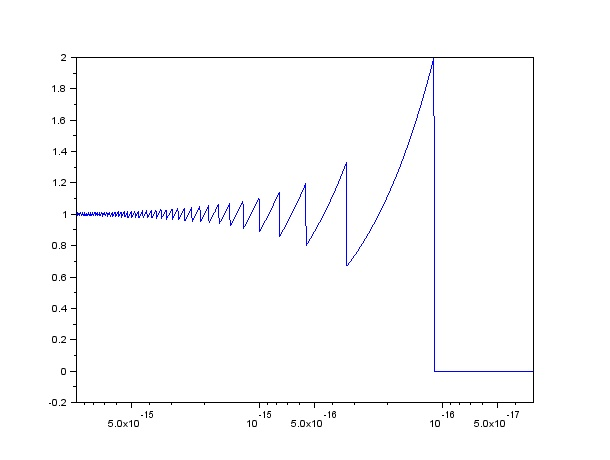
\includegraphics[width=0.8\textwidth]{./cap_aritmetica/pics/cancelamento_0}  
  \caption{Gráfico na função do exemplo~\ref{ex:cancelamento_0}.}
  \label{fig:cancelamento_0}
\end{figure}


\begin{figure}
  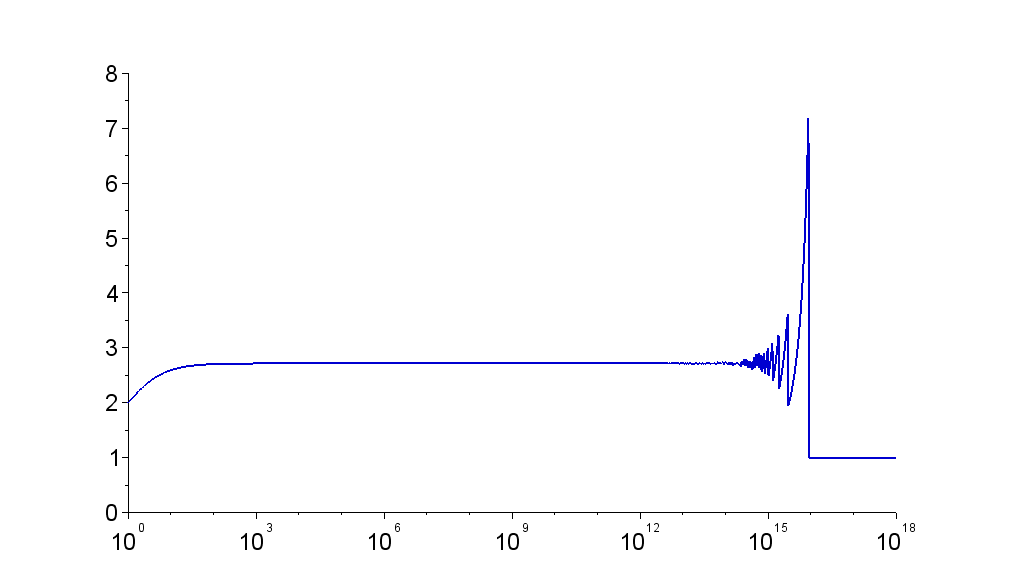
\includegraphics[width=0.8\textwidth]{./cap_aritmetica/pics/cancelamento_euler}
  \caption{Gráfico de $\left(1+\frac{1}{n}\right)^n$ em função de $n$ em escala linear-logarítmica variando de $10^0$ até $10^{18}$. Veja o exemplo~\ref{ex:cancelamento_euler}.}
  \label{fig:cancelamento_euler}
\end{figure}

\begin{ex}\label{ex:cancelamento_euler} Neste exemplo, estamos interessados em compreender mais detalhadamente o comportamento da expressão
\begin{equation*}
  \label{def_lim}\left(1+\frac{1}{n}\right)^n
\end{equation*}
quando $n$ é um número grande ao computá-la em sistemas de numeral de ponto flutuante com acurácia finita.
Um resultado bem conhecido do cálculo nos diz que o limite de (\ref{def_lim}) quando $n$ tende a infinito é o número de Euler:
\begin{equation*}\label{lim}
  \lim_{n\to \infty}\left(1+\frac{1}{n}\right)^n=e= 2,718281828459...
\end{equation*}

Sabemos também que a sequência produzida por \eqref{def_lim} é crescente, isto é:
$$\left(1+\frac{1}{1}\right)^1< \left(1+\frac{1}{2}\right)^2< \left(1+\frac{1}{3}\right)^3 < \cdots $$

No entanto, quando calculamos essa expressão no \verb+Scilab+, nos defrontamos com o seguinte resultado:
\begin{center}
\begin{tabular}{|c|c|c|c|c|}\hline &&&&\\[-0.3cm]
$n$ & $\left(1+\frac{1}{n}\right)^n$&$~~~~$&$n$ & $\left(1+\frac{1}{n}\right)^n$\\ &&&&\\[-0.3cm]\hline\\[-0.3cm]
$1$ & $2,0000000000000$ && $10^{2}$ & $2,7048138294215$ \\
$2$ & $2,2500000000000$ && $10^{4}$ & $2,7181459268249$ \\
$3$ & $2,3703703703704$ && $10^{6}$ & $2,7182804690957$ \\
$4$ & $2,4414062500000$ && $10^{8}$ & $2,7182817983391$ \\
$5$ & $2,4883200000000$ && $10^{10}$ & $2,7182820532348$ \\
$6$ & $2,5216263717421$ && $10^{12}$ & $2,7185234960372$ \\
$7$ & $2,5464996970407$ && $10^{14}$ & $2,7161100340870$ \\
$8$ & $2,5657845139503$ && $10^{16}$ & $1,0000000000000$ \\
$9$ & $2,5811747917132$ && $10^{18}$ & $1,0000000000000$ \\
$10$ & $2,5937424601000$ && $10^{20}$ & $1,0000000000000$ \\\hline
\end{tabular}  
\end{center}

Podemos resumir esses dados no gráfico de $\left(1+\frac{1}{n}\right)^n$ em função de $n$, veja a figura~\ref{fig:cancelamento_euler}.

Observe que quando $n$ se torna grande, da ordem de $10^{15}$, o gráfico da função deixa de se crescente e apresenta oscilações.  Observe também que a expressão se torna identicamente igual a $1$ depois de um certo limiar. Tais fenômenos não são intrínsecos da função $f(n)=(1+1/n)^n$, mas \emph{\uline{oriundas de erros de arredondamento}}, isto é, são resultados numéricos espúrios. A fim de pôr o comportamento numérico de tal expressão, apresentamos abaixo o gráfico da mesma função, porém restrito à região entre $10^{14}$ e $10^{16}$.

Para compreendermos melhor por que existe um limiar $N$ que, quando atingido torna a expressão do exemplo acima identicamente igual a $1$, observamos a sequência de operações realizadas pelo computador:
\begin{equation}\label{seq_oper}
n~\to ~1/n ~\to ~1+1/n ~\to ~(1+1/n)^n
\end{equation}
Devido ao limite de precisão da representação de números em ponto flutuante, existe um menor número representável que é maior do que 1. Este número é $1 + $\verb+eps+, onde \verb+eps+ é chamado de \emph{épsilon de máquina} e é o menor número que somado a 1 produz um resultado superior a 1 no sistema de numeração usado. O épsilon de máquina no sistema de numeração \emph{double} vale aproximadamente $2,22\times 10^{-16}$.
%%%%%%%%%%%%%%%%%%%%%%
% scilab
%%%%%%%%%%%%%%%%%%%%%%
\ifisscilab
No \verb+Scilab+, o epsilon de máquina é a constante \verb+eps+. Observe que:
\begin{verbatim}
-->1+%eps
 ans  =
    1.0000000000000002220446 
\end{verbatim}
\fi
%%%%%%%%%%%%%%%%%%%%%%
%%%%%%%%%%%%%%%%%%%%%%
% octave
%%%%%%%%%%%%%%%%%%%%%%
\ifisoctave
No \verb+GNU Octave+, o epsilon de máquina é a constante \verb+eps+. Observe que:
\begin{verbatim}
>> printf('%1.25f\n', 1+eps)
1.0000000000000002220446049
\end{verbatim}
\fi
%%%%%%%%%%%%%%%%%%%%%%
%%%%%%%%%%%%%%%%%%%%%%
% python
%%%%%%%%%%%%%%%%%%%%%%
\ifispython
Em \verb+Python+ podemos obter o epsilon de máquina com o seguinte comando \verb+numpy+:
\begin{verbatim}
>>> eps = np.finfo(float).eps
>>> print(eps)
2.22044604925e-16
>>> 1+eps == 1
False
>>> 1+eps
1.0000000000000002
\end{verbatim}
\fi
%%%%%%%%%%%%%%%%%%%%%%
Quando somamos a $1$ um número positivo inferior ao épsilon de máquina, obtemos o número 1. Dessa forma, o resultado obtido pela operação de ponto flutuante $1+n$ para $0<n<2,22 \times 10^{-16}$ é 1. 

Portanto, quando realizamos a sequência de operações dada em \eqref{seq_oper}, toda informação contida no número $n$ é perdida na soma com $1$ quando $1/n$ é menor que o épsilon de máquina, o que ocorre quando $n>5\times 10^{15}$. Assim, $(1+1/n)$ é aproximado para $1$ e a última operação se resume a $1^n$, o que é igual a $1$ mesmo quando $n$ é grande.

Um erro comum é acreditar que o perda de significância se deve ao fato de $1/n$ ser muito pequeno para ser representado e é aproximando para $0$. Isto é falso, o sistema de ponto de flutuante permite representar números de magnitude muito inferior ao épsilon de máquina. O problema surge da limitação no tamanho da mantissa. Observe como a seguinte sequência de operações não perde significância para números positivos x muito menores que o épsilon de máquina:
\begin{equation}\label{seq_oper2}
n ~\to ~1/n ~\to ~1/(1/n) 
\end{equation}
compare o desempenho numérico desta sequência de operações para valores pequenos de $n$ com o da seguinte sequência:
\begin{equation}\label{seq_oper3}
n ~\to ~1+n ~\to ~(1+n)-1.
\end{equation}
Finalmente, notamos que quando tentamos calcular $\left(1+\frac{1}{n}\right)^n$ para $n$ grande, existe perda de significância no cálculo de $1+1/n$. 
%%%%%%%%%%%%%%%%%%%%
% scilab
%%%%%%%%%%%%%%%%%%%%
\ifisscilab
Para entendermos isso melhor, vejamos o que acontece no \verb+Scilab+ quando $n=7\times 10^{13}$:
\begin{verbatim}
-->n=7e13
 n  =
     7.000000000000000000D+13  
-->1/n
 ans  =
     1.428571428571428435D-14   
-->y=1+1/n
 y  =
    1.000000000000014211D+00  
\end{verbatim}
Observe a perda de informação ao deslocar a mantissa de $1/n$. Para evidenciar o fenômenos, observamos o que acontece quando tentamos recalcular $n$ subtraindo $1$ de $1+1/n$ e invertendo o resultado:
\begin{verbatim}
-->y-1
 ans  =
     1.421085471520200372D-14   
-->1/(y-1)
 ans  =
     7.036874417766400000D+13  
\end{verbatim}
\fi
%%%%%%%%%%%%%%%%%%%%
%%%%%%%%%%%%%%%%%%%%
% octave
%%%%%%%%%%%%%%%%%%%%
\ifisoctave
Para entendermos isso melhor, vejamos o que acontece no \verb+GNU Octave+ quando $n=7\times 10^{13}$:
\begin{verbatim}
>> format('long')
>> n=7e13
n =  70000000000000
>> 1/n
ans =    1.42857142857143e-14
>> y=1+1/n
y =  1.00000000000001
\end{verbatim}
Observe a perda de informação ao deslocar a mantissa de $1/n$. Para evidenciar o fenômenos, observamos o que acontece quando tentamos recalcular $n$ subtraindo $1$ de $1+1/n$ e invertendo o resultado:
\begin{verbatim}
>> y-1
ans =    1.42108547152020e-14
>> 1/(y-1)
ans =  70368744177664
\end{verbatim}
\fi
%%%%%%%%%%%%%%%%%%%%
%%%%%%%%%%%%%%%%%%%%
% python
%%%%%%%%%%%%%%%%%%%%
\ifisscilab
Para entendermos isso melhor, vejamos o que acontece no \verb+Scilab+ quando $n=7\times 10^{13}$:
\begin{verbatim}
>>> n=7e13; print("%1.15e" % n)
7.000000000000000e+13
>>> n=7e13; print("%1.20e" % n)
7.00000000000000000000e+13
>>> print("%1.20e" % (1/n))
1.42857142857142843451e-14
>>> y=1+1/n; print("%1.20e" % y)
1.00000000000001421085e+00
\end{verbatim}
Observe a perda de informação ao deslocar a mantissa de $1/n$. Para evidenciar o fenômenos, observamos o que acontece quando tentamos recalcular $n$ subtraindo $1$ de $1+1/n$ e invertendo o resultado:
\begin{verbatim}
>>> print("%1.20e" % (y-1))
1.42108547152020037174e-14
>>> print("%1.20e" % (1/(y-1)))
7.03687441776640000000e+13
\end{verbatim}
\fi
%%%%%%%%%%%%%%%%%%%%
\end{ex}

\begin{ex}[Analogia da balança] Observe a seguinte comparação interessante que pode ser feita para ilustrar os sistemas de numeração com ponto fixo e flutuante: o sistema de ponto fixo é como uma balança cujas marcas estão igualmente espaçadas; o sistema de ponto flutuante é como uma balança cuja distância entre as marcas é proporcional à massa medida. Assim, podemos ter uma balança de ponto fixo cujas marcas estão sempre distanciadas de $100$g ($100$g, $200$g, $300$g, ..., $1$Kg, $1,1$Kg,...) e outra balança de ponto flutuante cujas marcas estão distanciadas sempre de aproximadamente um décimo do valor lido ($100$g, $110$g, $121$g, $133$g, ..., $1$Kg, $1,1$Kg, $1,21$Kg, ...) A balança de ponto fixo apresenta uma resolução baixa para pequenas medidas, porém uma resolução alta para grandes medidas. A balança de ponto flutuante distribui a resolução de forma proporcional ao longo da escala.    

Seguindo nesta analogia, o fenômeno de perda de significância pode ser interpretado como a seguir: imagine que você deseje obter o peso de um gato (aproximadamente $4$Kg). Dois processos estão disponíveis: colocar o gato diretamente na balança ou medir seu peso com o gato e, depois, sem o gato. Na balança de ponto flutuante, a incerteza associada na medida do peso do gato (sozinho) é aproximadamente $10\%$ de $4$Kg, isto é, $400$g. Já a incerteza associada à medida da uma pessoa (aproximadamente $70$Kg) com o gato é de $10\%$ do peso total, isto é, aproximadamente $7$Kg. Esta incerteza é da mesma ordem de grandeza da medida a ser realizada, tornado o processo impossível de ser realizado, já que teríamos uma incerteza da ordem de $14$Kg (devido à dupla medição) sobre uma grandeza de $4$Kg.    
\end{ex}

\subsection*{Exercícios}

\begin{exer} Considere as expressões:
  \begin{equation*}
    \frac{\exp(1/\mu)}{1+\exp(1/\mu)}  
  \end{equation*}
e
\begin{equation*}
  \frac{1}{\exp(-1/\mu)+1}
\end{equation*}
com $\mu>0$. Verifique que elas são idênticas como funções reais. Teste no computador cada uma delas para $\mu=0,1$, $\mu=0,01$ e $\mu=0,001$. Qual dessas expressões é mais adequada quando $\mu$ é um número pequeno? Por quê?
\end{exer}
\begin{resp}
  
  Quando $\mu$ é pequeno, $e^{1/\mu}$ é um número grande. A primeira expressão produz um ''overflow'' (número maior que o máximo representável) quando $\mu$ é pequeno. A segunda expressão, no entanto, reproduz o limite $1$ quando $\mu\to 0+$.
  
\end{resp}

\begin{exer} Encontre expressões alternativas para calcular o valor das seguintes funções quando $x$ é próximo de zero.
\begin{itemize}
\item[a)] $f(x)=\frac{1-\cos(x)}{x^2}$
\item[b)] $g(x)=\sqrt{1+x}-1$
\item[c)] $h(x)=\sqrt{x+10^6}-10^3$
\item[d)] $i(x)=\sqrt{1+e^{x}}-\sqrt{2}$ ~~~~~~ Dica: Faça $y=e^{x}-1$
\end{itemize}
\end{exer}
\begin{resp}
  
    a)~$\frac{1}{2}+\frac{x^2}{4!}+O(x^4)$; b)~$x/2+O(x^2)$; c)~$5\cdot 10^{-4}x+O(x^2)$; d)~$\frac{\sqrt{2}}{4}y+O(y^{2})=\frac{\sqrt{2}}{4}x+O(x^2)$
  
\end{resp}

\begin{exer} Use uma identidade trigonométrica adequada para mostrar que:
  \begin{equation*}
    \frac{1-\cos(x)}{x^2}= \frac{1}{2} \left(\frac{\sin(x/2)}{x/2}\right)^2.
  \end{equation*}
Analise o desempenho destas duas expressões no computador quando $x$ vale $10^{-5}$, $10^{-6}$, $10^{-7}$, $10^{-8}$, $10^{-9}$, $10^{-200}$ e $0$. Discuta o resultado.
\emph{Dica:} Para $|x|<10^{-5}$, $f(x)$ pode ser aproximada por $1/2-x^2/24$ com erro de truncamento inferior a $10^{-22}$.
\end{exer}

%\begin{exer} Considere a expressão
%$$
%f(x)=\frac{1-\cos(x)}{x^2}
%$$
%para $x$ pequeno. Verifique que
%$$
%\lim_{x\to 0}f(x)=0,5
%$$
%Depois calcule no \verb+Scilab+ $f(x)$ para $x=10^{-5}$, $x=10^{-6}$, $x=10^{-7}$, $x=10^{-8}$, $x=10^{-9}$ e $x=10^{-10}$. Finalmente, faça uma %aproximação analítica que elimine o efeito catastrófico.
%\end{exer}
%%Redundante


\begin{exer} Reescreva as expressões:
  $$\sqrt{e^{2x}+1}-e^x \qquad\text{e}\qquad \sqrt{e^{2x}+x^2}-e^x $$
  de modo que seja possível calcular seus valores para $x=100$ utilizando a aritmética de ponto flutuante ("Double") no computador.
\end{exer}

\begin{exer} Na teoria da relatividade restrita, a energia cinética de uma partícula e sua velocidade se relacionam pela seguinte fórmula:
  \begin{equation*}
    E=mc^2\left(\frac{1}{\sqrt{1-(v/c)^2}}-1\right),
  \end{equation*}
onde $E$ é a energia cinética da partícula, $m$ é a massa de repouso, $v$ o módulo da velocidade e $c$ a velocidade da luz no vácuo dada por $c=299792458 m/s$. Considere que a massa de repouso $m=9,10938291\times 10^{-31} Kg$ do elétron seja conhecida com erro relativo de $10^{-9}$. Qual é o valor da energia e o erro relativo associado a essa grandeza quando $v=0,1 c$, $v=0,5 c$, $v=0,99c$ e $v=0,999c$ sendo que a incerteza relativa na medida da velocidade é $10^{-5}$?
\end{exer}
\begin{resp}
  
    $4,12451228\times 10^{-16}$~J; $0,002\%$; $0,26654956\times 10^{-14}$~J; $0,002\%$; $4,98497440\times 10^{-13}$~J; $0,057\%$; $1,74927914\times 10^{-12}$~J; $0,522\%$.
  
\end{resp}

\begin{exer} Deseja-se medir a concentração de dois diferentes oxidantes no ar. Três sensores eletroquímicos estão disponíveis para a medida e apresentam a seguintes respostas:
$$v_1= 270 [A] +  30 [B],~~~ v_2= 140 [A] +  20 [B] ~~ \text{e}~~ v_3= 15 [A] +  200 [B]$$
as tensões $v_1$, $v_2$ e $v_3$ são dadas em $mV$ e as concentrações em $milimol/l$.
\begin{itemize}
\item [a)] Encontre uma expressão para os valores de $[A]$ e $[B]$ em termos de $v_1$ e $v_2$ e, depois, em termos de $v_1$ e $v_3$. Dica:
Se $ad\neq bc$, então a matriz $A$ dada por
$$A=\begin{bmatrix}a&b\\c&d\end{bmatrix}$$
é inversível e sua inversa é dada por
$$A^{-1}= \frac{1}{ad-bc} \left[\begin{array}{cc}d&-b\\-c&a\end{array}\right].$$

\item[b)] Sabendo que incerteza relativa associada às sensibilidades dos sensores 1 e 2 é de $2\%$ e que a incerteza relativa associada às sensibilidades do sensor 3 é $10\%$, verifique a incerteza associada à medida feita com o par $1-2$ e o par $1-3$. Use $[A]=[B]=10milimol/l$. Dica: Você deve diferenciar as grandezas $[A]$ e $[B]$ em relação aos valores das tensões.
\end{itemize}
\end{exer}
\begin{resp}
  
Em ambos casos, temos a seguinte estrutura:
$$\begin{bmatrix}
S_{11}& S_{12}\\
S_{21}& S_{22}
\end{bmatrix} 
\begin{bmatrix}
\left[ A\right]\\
\left[ B\right]
\end{bmatrix} 
= 
\begin{bmatrix}
v_1\\
v_2
\end{bmatrix}$$
De forma que
$$\begin{bmatrix}
\left[ A\right]\\
\left[ B\right]
\end{bmatrix}
=\begin{bmatrix}
S_{11}& S_{12}\\
S_{21}& S_{22}
\end{bmatrix}^{-1}
\begin{bmatrix}
v_1\\
v_2
\end{bmatrix}
= \frac{1}{S_{11}S_{22}-S_{12}S_{21}}
\begin{bmatrix}
S_{22}& -S_{12}\\
-S_{21}& S_{11}
\end{bmatrix}
\begin{bmatrix}
v_1\\
v_2
\end{bmatrix}
$$
Portanto
\begin{eqnarray*}
[ A ]&=&\frac{S_{22}v_1-S_{12}v_2}{S_{11}S_{22}-S_{12}S_{21}}\\
\left[ {B} \right]&=&\frac{-S_{21}v_1+S_{11}v_2}{S_{11}S_{22}-S_{12}S_{21}}
\end{eqnarray*}

Usando derivação logarítmica, temos

\begin{eqnarray*}
\frac{1}{[ A ]}\frac{\partial [ A ]}{\partial S_{11}}&=&-\frac{S_{22}}{S_{11}S_{22}-S_{12}S_{21}}\\
\frac{1}{[ A ]}\frac{\partial [ A ]}{\partial S_{12}}&=&-\frac{v_2}{S_{22}v_1-S_{12}v_2}+\frac{S_{21}}{S_{11}S_{22}-S_{12}S_{21}}=-\frac{[A]}{\left[B\right]}\cdot \frac{S_{22}}{S_{11}S_{22}-S_{12}S_{21}}\\
\frac{1}{[ A ]}\frac{\partial [ A ]}{\partial S_{21}}&=&\frac{S_{12}}{S_{11}S_{22}-S_{12}S_{21}}\\
\frac{1}{[ A ]}\frac{\partial [ A ]}{\partial S_{22}}&=&\frac{v_1}{S_{22}v_1-S_{12}v_2}-\frac{S_{11}}{S_{11}S_{22}-S_{12}S_{21}}=\frac{[A]}{\left[B\right]}\cdot \frac{S_{12}}{S_{11}S_{22}-S_{12}S_{21}}
\end{eqnarray*}
e
\begin{eqnarray*}
\frac{1}{\left[ B \right]}\frac{\partial \left[ B \right]}{\partial S_{11}}&=&\frac{v_2}{-S_{21}v_1+S_{11}v_2}-\frac{S_{22}}{S_{11}S_{22}-S_{12}S_{21}}=\frac{\left[B\right]}{[A]} \frac{S_{21}}{S_{11}S_{22}-S_{12}S_{21}}\\
\frac{1}{\left[ B \right]}\frac{\partial \left[ B \right]}{\partial S_{12}}&=&\frac{S_{21}}{S_{11}S_{22}-S_{12}S_{21}}\\
\frac{1}{\left[ B \right]}\frac{\partial \left[ B \right]}{\partial S_{21}}&=&-\frac{v_1}{-S_{21}v_1+S_{11}v_2}+\frac{S_{21}}{S_{11}S_{22}-S_{12}S_{21}}=-\frac{\left[B\right]}{[A]}\frac{S_{11}}{S_{11}S_{22}-S_{12}S_{21}}\\
\frac{1}{\left[ B \right]}\frac{\partial \left[ B \right]}{\partial S_{22}}&=&-\frac{S_{11}}{S_{11}S_{22}-S_{12}S_{21}}\\
\end{eqnarray*}


E o erro associado às medidas pode ser aproximado por
\begin{eqnarray*}
\frac{1}{[A]}\delta_{[A]}&=&\left|\frac{1}{[ A ]}\frac{\partial [ A ]}{\partial S_{11}}\right| \delta_{S_{11}}+\left|\frac{1}{[ A ]}\frac{\partial [ A ]}{\partial S_{12}}\right| \delta_{S_{12}}+\left|\frac{1}{[ A ]}\frac{\partial [ A ]}{\partial S_{21}}\right| \delta_{S_{21}}+\left|\frac{1}{[ A ]}\frac{\partial [ A ]}{\partial S_{22}}\right| \delta_{S_{22}}\\
&=&\frac{1}{\left|\det{S}\right|}\left[S_{22}\delta_{S_{11}}+\frac{[A]}{\left[B\right]}S_{22}\delta_{S_{12}}+S_{12}\delta_{S_{21}}+\frac{[A]}{\left[B\right]}S_{12}\delta_{S_{22}}\right]
\end{eqnarray*}
Analogamente, temos:
\begin{eqnarray*}
\frac{1}{[B]}\delta_{[B]}&=&\frac{1}{\left|\det{S}\right|}\left[\frac{[B]}{\left[A\right]}S_{21}\delta_{S_{11}}+S_{21}\delta_{S_{11}}+\frac{\left[B\right]}{[A]}S_{11}\delta_{S_{21}}+S_{11}\delta_{S_{22}}\right]
\end{eqnarray*}

onde não se indicou $|S_{ij}|$ nem $|[.]|$ pois são todos positivos.


Fazemos agora a aplicação numérica:

{\bf Caso do par 1-2:}
$$\det{S}=\left|\begin{matrix}270&30\\140&20\end{matrix}\right|=1200$$
\begin{eqnarray*}
\frac{1}{[A]}\delta_{[A]}
&=&\frac{1}{1200}\left[20\times 270\times 2\%+20\times 30\times 2\%+30\times 140\times 2\%+30\times 20\times 2\%\right]\\&=&\frac{216}{1200}=0.18=18\%\\
\frac{1}{[B]}\delta_{[B]}
&=&\frac{1}{1200}\left[140\times 270\times 2\%+140\times 30\times 2\%+270\times 140\times 2\%+270\times 20\times 2\%\right]\\&=&\frac{426}{1200}=0.355=35.5\%
\end{eqnarray*}

{\bf Caso do par 1-3:}
$$\det{S}=\left|\begin{array}{cc}270&30\\15&200\end{array}\right|=53550$$
\begin{eqnarray*}
\frac{1}{[A]}\delta_{[A]}
&=&\frac{1}{53550}\left[200\times 270\times 2\%+200\times 30\times 2\%+30\times 15\times 10\%+30\times 200\times 10\%\right]\\&=&\frac{1804,6}{52550}\approx 0.0337=3.37\%\\
\frac{1}{[B]}\delta_{[B]}
&=&\frac{1}{53550}\left[15\times 270\times 2\%+15\times 30\times 2\%+270\times 15\times 10\%+270\times 200\times 10\%\right]\\&=&	\frac{5895}{53550}\approx   0.11=11\%
\end{eqnarray*}

Conclusão, apesar de o sensor $3$ apresentar uma incerteza cinco vezes maior na sensibilidade, a escolha do sensor $3$ para fazer par ao sensor $1$ parece mais adequada.    
  
\end{resp}

%\end{document} 

%Este trabalho está licenciado sob a Licença Creative Commons Atribuição-CompartilhaIgual 3.0 Não Adaptada. Para ver uma cópia desta licença, visite http://creativecommons.org/licenses/by-sa/3.0/ ou envie uma carta para Creative Commons, PO Box 1866, Mountain View, CA 94042, USA.

%\documentclass[main.tex]{subfiles}
%\begin{document}

\chapter{Solução de equações de uma variável}\index{equações!de uma variável}

Neste capítulo, construiremos aproximações numéricas para a solução de \emph{equações algébricas em uma única variável real}. Observamos que obter uma solução para uma tal dada equação é equivalente a encontrar um \emph{zero de uma função real}\index{função!zero de}\index{função!raiz de} apropriada. Com isso, iniciamos este capítulo discutindo condições de existência e unicidade de raízes de funções de uma variável real. Então, apresentamos o \emph{método da bisseção}\index{método da bisseção} como uma primeira abordagem numérica para a solução de tais equações.

Em seguida, exploramos outra abordagem via \emph{iteração do ponto fixo}\index{iteração do ponto fixo}. Desta, obtemos o \emph{método de Newton}\footnote{Sir Isaac Newton, 1642 - 1727, matemático e físico inglês.}\index{método de Newton}, para o qual estudamos aplicações e critérios de convergência. Por fim, apresentamos o \emph{método das secantes}\index{método das secantes} como uma das possíveis variações do método de Newton.

%%%%%%%%%%%%%%%%%%%%
% python
%%%%%%%%%%%%%%%%%%%%
\ifispython
Ao longo do capítulo, apresentamos algumas computações com \verb+Python+. Nestas, assumiremos o que os seguintes módulos estão carregados:
\begin{verbatim}
>>> from __future__ import division
>>> import numpy as np
>>> import matplotlib.pyplot as plt
>>> import scipy as sci
>>> from scipy import optimize
\end{verbatim}
A segunda instrução carrega a biblioteca de computação científica \href{http://www.numpy.org/}{numpy} e a terceira carrega a biblioteca gráfica \href{http://matplotlib.org/}{matplotlib}.
\fi

\section{Existência e unicidade}\index{função!}\index{função!zero}

O \emph{teorema de Bolzano}\footnote{Bernhard Placidus Johann Gonzal Nepomuk Bolzano, 1781 - 1848, matemático do Reino da Boêmia.}\index{teorema de!Bolzano} nos fornece condições suficientes para a existência do zero de uma função. Este é uma aplicação direta do \emph{teorema do valor intermediário}\index{teorema do valor intermediário}.

\begin{teo}[Teorema de Bolzano]\label{teo:teorema_de_Bolzano}
  Se $f:[a, b]\to\mathbb{R}$, $y = f(x)$, é uma função contínua tal que $f(a)\cdot f(b) < 0$\footnote{Esta condição é equivalente a dizer que a função troca de sinal no intervalo.}, então existe $x^*\in (a, b)$ tal que $f(x^*) = 0$.
\end{teo}
\begin{proof}
  O resultado é uma consequência imediata do teorema do valor intermediário que estabelece que dada uma função contínua $f:[a, b]\to\mathbb{R}$, $y = f(x)$, tal que $f(a) < f(b)$ (ou $f(b) < f(a)$), então para qualquer $d\in \left(f(a), f(b)\right)$ (ou $k\in \left(f(b), f(a)\right)$) existe $x^*\in (a, b)$ tal que $f(x^*) = k$. Ou seja, nestas notações, se $f(a)\cdot f(b) < 0$, então $f(a) < 0 < f(b)$ (ou $f(b) < 0 < f(a)$). Logo, tomando $k = 0$, temos que existe $x^*\in (a, b)$ tal que $f(x^*) = k = 0$.
\end{proof}

Em outras palavras, se $f(x)$ é uma função contínua em um dado intervalo no qual ela troca de sinal, então ela têm pelo menos um zero neste intervalo (veja a Figura~\ref{fig:teorema_de_Bolzano}).

\begin{figure}
  \centering
  \includegraphics{./cap_equacao1d/pics/teorema_de_Bolzano/teorema_de_Bolzano.eps}
  \caption{Teorema de Bolzano.}
  \label{fig:teorema_de_Bolzano}
\end{figure}

% \begin{teo}[Teorema do Valor Intermediário]
% Se $f:[a,b]\to\mathbb{R}$ é um função contínua e $K$ for um número entre $f(a)$ e $f(b)$, então existe $c\in(a,b)$ para o qual $f(c)=K$.
% \end{teo}

% \begin{figure}[h!]
%   \centering
%   \includegraphics[scale=0.5]{./cap_equacao1d/pics/teorema_do_valor_intermediario/teorema_do_valor_intermediario.eps}
%   \caption{Teorema do valor intermediário}
%   \label{fig:teorema_do_valor_intermediario}
% \end{figure}

% Em particular, se $f(a)>0$ e $f(b)<0$, então $0\in [f(b),f(a)]$ e podemos garantir a existência de $c\in(a,b)$ tal que $f(c)=0$, isto é, existe uma raiz no intervalo $(a,b)$. A mesma afirmação é válida se $f(a)<0$ e $f(b)>0$. Em outras palavras, o teorema do Valor Intermediário afirma que uma função contínua não pode mudar de sinal sem passar por zero.

\begin{ex}\label{ex:teorema_de_Bolzano}
Mostre que existe pelo menos uma solução da equação $e^x=x+2$ no intervalo $(-2,0)$.
\end{ex}
\begin{sol}
Primeiramente, observamos que resolver a equação $e^x = x+2$ é equivalente a resolver $f(x) = 0$ com $f(x)=e^x-x-2$. Agora, como $f(-2)=e^{-2}>0$ e $f(0)=-2<0$, temos do teorema de Bolzano que existe pelo menos um zero de $f(x)$ no intervalo $(-2, 0)$. E, portanto, existe pelo menos uma solução da equação dada no intervalo $(-2, 0)$.

%%%%%%%%%%%%%%%%%%%%
% scilab
%%%%%%%%%%%%%%%%%%%%
\ifisscilab
Podemos usar o \verb+Scilab+ para estudarmos esta função. Por exemplo, podemos definir a função $f(x)$ e computá-la nos extremos do intervalo dado com os seguintes comandos:
\begin{verbatim}
-->deff('y=f(x)','y=exp(x)-x-2')
-->f(-2),f(0)
 ans  =
    0.1353353  
 ans  =
  - 1.  
\end{verbatim}
Alternativamente (e com maior precisão), podemos verificar diretamente o sinal da função nos pontos desejados com comando \verb+sign+:
\begin{verbatim}
-->sign(f(-2)),sign(f(0))
 ans  =
    1.  
 ans  =
  - 1.  
\end{verbatim}
\fi
%%%%%%%%%%%%%%%%%%%%
%%%%%%%%%%%%%%%%%%%%
% octave
%%%%%%%%%%%%%%%%%%%%
\ifisoctave
Podemos usar o \verb+GNU Octave+ para estudarmos esta função. Por exemplo, podemos definir a função $f(x)$ e computá-la nos extremos do intervalo dado com os seguintes comandos:
\begin{verbatim}
>> f = @(x) exp(x)-x-2
f = f(x) = exp(x)-x-2
>> f(-2),f(0)
ans =  0.13534
ans = -1
\end{verbatim}
Alternativamente (e com maior precisão), podemos verificar diretamente o sinal da função nos pontos desejados com comando \verb+sign+:
\begin{verbatim}
>> sign(f(-2)),sign(f(0))
ans =  1
ans = -1
\end{verbatim}
\fi
%%%%%%%%%%%%%%%%%%%%
%%%%%%%%%%%%%%%%%%%%
% python
%%%%%%%%%%%%%%%%%%%%
\ifispython
Podemos usar \verb+Python+ para estudarmos esta função. Por exemplo, podemos definir a função $f(x)$ e computá-la nos extremos do intervalo dado com os seguintes comandos:
\begin{verbatim}
>>> def f(x): return np.exp(x)-x-2
... 
>>> f(-2),f(0)
(0.13533528323661281, -1.0)
\end{verbatim}
Alternativamente (e com maior precisão), podemos verificar diretamente o sinal da função nos pontos desejados com a função \href{https://docs.scipy.org/doc/numpy/reference/generated/numpy.sign.html?highlight=numpy.sign#numpy.sign}{numpy.sign}:
\begin{verbatim}
>>> np.sign(f(-2)*f(0))
-1.0
\end{verbatim}
\fi
%%%%%%%%%%%%%%%%%%%%
\end{sol}


Quando procuramos aproximações para zeros de funções, é aconselhável isolar cada raiz em um intervalo. Desta forma, gostaríamos de poder garantir a existência e a unicidade da raiz dentro de um dado intervalo. A seguinte proposição nos fornece condições suficientes para tanto.

\begin{prop}\label{prop:existencia_e_unicidade}
Se $f:[a, b]\to\mathbb{R}$ é um função diferenciável, $f(a)\cdot f(b)<0$ e $f'(x)>0$ (ou $f'(x)<0$) para todo $x\in(a, b)$, então existe um único $x^*\in (a, b)$ tal que $f(x^*) = 0$.
\end{prop}

Em outras palavras, para garantirmos que exista um único zero de uma dada função diferenciável em um intervalo, é suficiente que ela troque de sinal e seja monótona neste intervalo.

\begin{ex}
No Exemplo~\ref{ex:teorema_de_Bolzano}, mostramos que existe pelo menos um zero de $f(x) = e^{x}-x-2$ no intervalo $(-2,0)$, pois $f(x)$ é contínua e $f(-2)\cdot f(0) < 0$. Agora, observamos que, além disso, $f'(x)=e^x-1$ e, portanto, $f'(x) < 0$ para todo $x\in(-2,0)$. Logo, da Proposição~\ref{prop:existencia_e_unicidade}, temos garantida a existência de um único zero no intervalo dado.

%%%%%%%%%%%%%%%%%%%%
% scilab
%%%%%%%%%%%%%%%%%%%%
\ifisscilab
Podemos inspecionar o comportamento da função $f(x)= e^x - x - 2$ e de sua derivada fazendo seus gráficos no Scilab. Para tanto, podemos fazer o seguinte teste:
\begin{verbatim}
-->x = linspace(-2,0,50);
-->deff('y = f(x)','y=exp(x)-x-2')  // define f
-->plot(x,f(x));xgrid               // grafico de f
-->deff('y = fl(x)','y=exp(x)-1')   // a derivada
-->plot(x,fl(x));xgrid              // grafico de f'
\end{verbatim}
\fi
%%%%%%%%%%%%%%%%%%%%
%%%%%%%%%%%%%%%%%%%%
% octave
%%%%%%%%%%%%%%%%%%%%
\ifisoctave
Podemos inspecionar o comportamento da função $f(x)= e^x - x - 2$ e de sua derivada fazendo seus gráficos no \verb+GNU Octave+. Para tanto, podemos fazer o seguinte teste:
\begin{verbatim}
>> xx = linspace(-2,0,50);
>> f = @(x) exp(x)-x-2  #define f
f = f(x) = exp(x)-x-2
>> plot(xx,f(xx))grid on;hold on #grafico de f
>> plot(xx,fl(xx)) #grafico de f'
\end{verbatim}
\fi
%%%%%%%%%%%%%%%%%%%%
%%%%%%%%%%%%%%%%%%%%
% python
%%%%%%%%%%%%%%%%%%%%
\ifispython
Podemos inspecionar o comportamento da função $f(x)= e^x - x - 2$ e de sua derivada fazendo seus gráficos no Python. Para tanto, podemos usar o seguinte código \verb+Python+:
\begin{verbatim}
>>> def f(x): return np.exp(x)-x-2
... 
>>> xx = np.linspace(-2,0)
>>> plt.plot(xx,f(xx))
>>> plt.grid(); plt.show()

>>> def fl(x): return np.exp(x)-1
... 
>>> plt.plot(xx,fl(xx))
>>> plt.grid(); plt.show()
\end{verbatim}
\fi
%%%%%%%%%%%%%%%%%%%%
\end{ex}

A discussão feita nesta seção, especialmente o teorema de Bolzano, nos fornece os fundamentos para o método da bisseção, o qual discutimos na próxima seção.

\subsection*{Exercícios}
\begin{exer}\label{exer:existencia_sol1}
  Mostre que $\cos x = x$ tem solução no intervalo $[0, \pi/2]$.
\end{exer}
\begin{resp}
  
  Observamos que a equação é equivalente a $\cos(x) - x = 0$. Tomando, então, $f(x) = \cos(x) - x$, temos que $f(x)$ é contínua em $[0, \pi/2]$, $f(0) = 1$ e $f(\pi/2) = -\pi/2 < 0$. Logo, do teorema de Bolzano~\ref{teo:teorema_de_Bolzano}, concluímos que a equação dada tem pelo menos uma solução no intervalo $(0, \pi/2)$.    
  
\end{resp}

\begin{exer}
  Mostre que $\cos x = x$ tem uma única solução no intervalo $[0, \pi/2]$.
\end{exer}
\begin{resp}
  
    No Exercício~\ref{exer:existencia_sol1}, mostramos que a função $f(x) = \cos(x) - x$ tem um zero no intervalo $[0, \pi/2]$. Agora, observamos que $f'(x) = -\sen(x) - 1$. Como $0 < \sen x < 1$ para todo $x\in (0, \pi/2)$, temos que $f'(x) < 0$ em $(0, \pi/2)$, isto é, $f(x)$ é monotonicamente decrescente neste intervalo. Logo, da Proposição~\ref{prop:existencia_e_unicidade}, temos que existe um único zero da função neste intervalo.
  
\end{resp}

\begin{exer} Interprete a equação $\cos(x)=kx$ como o problema de encontrar a intersecção da curva $y=\cos(x)$ com $y=kx$. Encontre o valor positivo $k$ para o qual essa equação admite exatamente duas raízes positivas distintas.
\end{exer}
\begin{resp}
  
    $k\approx 0,161228$
  
\end{resp}


\begin{exer}Mostre que a equação:
  \begin{equation*}
    \ln(x)+x^3-\frac{1}{x}=10  
  \end{equation*}
possui uma única solução positiva.
\end{exer}

\begin{exer}\label{exer:teorema_de_Bolzano_exatidao} Use o teorema de Bolzano para mostrar que o erro absoluto ao aproximar o zero da função $f(x)=e^x-x-2$ por $\overline{x}=-1,841$ é menor que $10^{-3}$.
\end{exer}
\begin{resp}
  
    Escolhendo o intervalo $[a, b] = [-1,841-10^{-3}, -1,841+10^{-3}]$, temos $f(a)\approx 5\times 10^{-4} > 0$ e $f(b)\approx -1,2\times 10^{-3} < 0$, isto é, $f(a)\cdot f(b) < 0$. Então, o teorema de Bolzano nos garante que o zero exato $x^*$ de $f(x)$ está no intervalo $(a, b)$. Logo, da escolha feita, $|-1,841 - x^*| < 10^{-3}$.
  
\end{resp}

\begin{exer} Mostre que o erro absoluto associado à aproximação $\overline{x} = 1,962$ para a solução exata $x^*$ de:
  \begin{equation*}
    e^x+\sin (x) +x = 10  
  \end{equation*}
é menor que $10^{-4}$.
\end{exer}
\begin{resp}
  Basta aplicar as ideias da solução do Exercício~\ref{exer:teorema_de_Bolzano_exatidao}.
\end{resp}

\begin{exer}\label{existe_unica} Mostre que a equação
  \begin{equation*}
    \ln(x)+x-\frac{1}{x}=v
  \end{equation*}
possui uma solução para cada $v$ real e que esta solução é única.
\end{exer}

\section{Método da bisseção}\index{método!da bisseção}

O \emph{método da bisseção} explora o fato de que uma função contínua $f:[a, b]\to \mathbb{R}$ com $f(a)\cdot f(b) < 0$ tem um zero no intervalo $(a, b)$ (veja o teorema de Bolzano~\ref{teo:teorema_de_Bolzano}). Assim, a ideia para aproximar o zero de uma tal função $f(x)$ é tomar, como primeira aproximação, o ponto médio do intervalo $[a, b]$, isto é:
\begin{equation*}
  x^{(0)} = \frac{(a + b)}{2}. 
\end{equation*}
Pode ocorrer de $f(x^{(0)}) = 0$ e, neste caso, o zero de $f(x)$ é $x^* = x^{(0)}$. Caso contrário, se $f(a)\cdot f(x^{(0)}) < 0$, então $x^*\in (a, x^{(0)})$. Neste caso, tomamos como segunda aproximação do zero de $f(x)$ o ponto médio do intervalo $[a, x^{(0)}]$, isto é, $x^{(1)} = (a + x^{(0)})/2$. Noutro caso, temos $f(x^{(0)})\cdot f(b) < 0$ e, então, tomamos $x^{(1)} = (x^{(0)} + b)/2$. Repetimos este procedimento até obtermos a aproximação desejada (veja Figura~\ref{fig:metodo_da_bissecao}).
 
\begin{figure}
  \centering
  \includegraphics{./cap_equacao1d/pics/metodo_da_bissecao/metodo_da_bissecao.eps}
  \caption{Método da bisseção.}
  \label{fig:metodo_da_bissecao}
\end{figure}

De forma mais precisa, suponha que queiramos calcular uma aproximação com uma certa precisão $TOL$ para um zero $x^*$ de uma dada função contínua $f:[a, b]\to\mathbb{R}$ tal que $f(a)\cdot f(b) < 0$. Iniciamos, tomando $n=0$ e:
\begin{equation*}
  a^{(n)} = a,\quad b^{(n)} = b\quad\text{e}\quad x^{(n)} = \frac{a^{(n)} + b^{(n)}}{2}.
\end{equation*}
Verificamos o \emph{critério de parada}\index{critério de parada}, isto é, se $f(x^{(n)}) = 0$ ou:
\begin{equation*}
  \displaystyle \frac{|b^{(n)} - a^{(n)}|}{2} < TOL,
\end{equation*}
então $x^{(n)}$ é a aproximação desejada. Caso contrário, preparamos a próxima iteração $n+1$ da seguinte forma: se $f(a^{(n)})\cdot f(x^{(n)}) < 0$, então definimos $a^{(n+1)} = a^{(n)}$ e $b^{(n+1)} = x^{(n)}$; noutro caso, se $f(x^{(n)})\cdot f(b^{(n)}) < 0$, então definimos $a^{(n+1)} = x^{(n)}$ e $b^{(n+1)} = b^{(n)}$. Trocando $n$ por $n+1$, temos a nova aproximação do zero de $f(x)$ dada por:
\begin{equation*}
  x^{(n+1)} = \frac{a^{(n+1)} + b^{(n+1)}}{2}.
\end{equation*}
Voltamos a verificar o critério de parada acima e, caso não satisfeito, iteramos novamente. Iteramos até obtermos a aproximação desejada ou o número máximo de iterações ter sido atingido.

\begin{ex}\label{ex:metodo_da_bissecao}Use o método da bisseção para calcular uma solução de $e^x = x + 2$ no intervalo $[-2, 0]$ com precisão $TOL = 10^{-1}$.
\end{ex}
\begin{sol}
  Primeiramente, observamos que resolver a equação dada é equivalente a calcular o zero de $f(x) = e^x - x - 2$. Além disso, temos $f(-2)\cdot f(0) < 0$. Desta forma, podemos iniciar o método da bisseção tomando o intervalo inicial $[a^{(0)}, b^{(0)}] = [-2, 0]$ e:
  \begin{equation*}
    x^{(0)} = \frac{a^{(0)} + b^{(0)}}{2} = -1.
  \end{equation*}
  Apresentamos as iterações na Tabela~\ref{tab:metodo_da_bissecao}. Observamos que a precisão $TOL = 10^{-1}$ foi obtida na quarta iteração com o zero de $f(x)$ sendo aproximado por $x^{(4)} = 1,8125$.
  \begin{table}
    \centering
    \caption{Iteração do método da bisseção para o Exemplo~\ref{ex:metodo_da_bissecao}.}
    \label{tab:metodo_da_bissecao}
    \begin{tabular}{l|ccc|c|c}\hline
      $n$ & $a^{(n)}$ & $b^{(n)}$ & $x^{(n)}$ & $f(a^{(n)})f(x^{(n)})$ & $\displaystyle \frac{|b^{(n)}-a^{(n)}|}{2}$\\\hline
      $0$ & $-2$ & $0$ & $-1$ & $< 0$ & $1$\\
      $1$ & $-2$ & $-1$ & $-1,5$ & $<0$ & $0,5$\\
      $2$ & $-2$ & $-1,5$ & $-1,75$ & $<0$ & $0,25$\\
      $3$ & $-2$ & $-1,75$ & $-1,875$ & $>0$ & $0,125$\\
      $4$ & $-1,875$ & $-1,75$ & $-1,8125$ & $<0$ & $0,0625$\\\hline
    \end{tabular}
  \end{table}
  
%%%%%%%%%%%%%%%%%%%%
% scilab
%%%%%%%%%%%%%%%%%%%%
\ifisscilab
Usando o \verb+Scilab+ neste exemplo, temos:
\begin{verbatim}
-->deff('y = f(x)','y = exp(x) - x - 2')
-->a=-2, b=0, x=(a+b)/2, TOL = (b-a)/2, sign(f(a)*f(x))
-->b=x, x=(a+b)/2, TOL = (b-a)/2, sign(f(a)*f(x))
\end{verbatim}
  e, assim, sucessivamente. Veja o código completo na Seção~\ref{subsec:codigo_bissecao}.
\fi    
%%%%%%%%%%%%%%%%%%%%
%%%%%%%%%%%%%%%%%%%%
% octave
%%%%%%%%%%%%%%%%%%%%
\ifisoctave
Usando o \verb+GNU Octave+ neste exemplo, temos:
\begin{verbatim}
>> f = @(x) exp(x) - x - 2
f = f(x) = exp(x) - x - 2
>> a=-2, b=0, x=(a+b)/2, TOL = (b-a)/2, sign(f(a)*f(x))
a = -2
b = 0
x = -1
TOL =  1
ans = -1
>> b=x, x=(a+b)/2, TOL = (b-a)/2, sign(f(a)*f(x))
b = -1
x = -1.5000
TOL =  0.50000
ans = -1
\end{verbatim}
e, assim, sucessivamente. Veja o código completo na Seção~\ref{subsec:codigo_bissecao}.
\fi    
%%%%%%%%%%%%%%%%%%%%
%%%%%%%%%%%%%%%%%%%%
% python
%%%%%%%%%%%%%%%%%%%%
\ifispython
Usando \verb+Python+ neste exemplos, temos:
\begin{verbatim}
>>> def f(x): return np.exp(x) - x - 2
... 
>>> a=-2; b=0; x = (a+b)/2; [a,b,x]
[-2, 0, -1.0]
>>> [(b-a)/2, np.sign(f(a)*f(x))]
[1.0, -1.0]
>>> b=x; x=(a+b)/2; [a,b,x]
[-2, -1.0, -1.5]
>>> [(b-a)/2, np.sign(f(a)*f(x))]
\end{verbatim}
e, assim, sucessivamente. Veja o código completo na Seção~\ref{subsec:codigo_bissecao}.
\fi    
%%%%%%%%%%%%%%%%%%%%
\end{sol}

Vamos agora discutir sobre a \emph{convergência} do método da bisseção. O próximo Teorema~\ref{teo:convergencia_bissecao} nos garante a convergência do método da bisseção.

\begin{teo}[Convergência do método da bisseção]\label{teo:convergencia_bissecao} Sejam $f:[a, b]\to \mathbb{R}$ uma função contínua tal que $f(a)\cdot f(b) < 0$ e $x^*$ o único zero de $f(x)$ no intervalo $(a, b)$. Então, a sequência $\{x^{(n)}\}_{n>=0}$ do método da bisseção satisfaz:
  \begin{equation*}
    |x^{(n)} - x^{*}| < \frac{b - a}{2^{n+1}},\quad\forall n\geq 0,
  \end{equation*}
isto é, $x^{(n)}\to x^*$ quando $n\to\infty$.
\end{teo}
\begin{proof}
 Notemos que, a cada iteração, a distância entre a aproximação $x^{(n)}$ e o zero $x^*$ da função é menor ou igual que a metade do tamanho do intervalo $[a^{(n)}, b^{(n)}]$ (veja Figura~\ref{fig:metodo_da_bissecao}), isto é:
\begin{equation*}
  |x^{(n)}-x^*| \leq \frac{b^{(n)}-a^{(n)}}{2}.
\end{equation*}
Por construção do método, temos $[a^{(n)}, b^{(n)}]\subset [a^{(n-1)}, b^{(n-1)}]$ e:
\begin{equation*}
  b^{(n)} - a^{(n)} = \frac{b^{(n-1)}-a^{(n-1)}}{2}.
\end{equation*}
Desta forma:
\begin{equation*}
  |x^{(n)}-x^*|  \leq \frac{b^{(n)}-a^{(n)}}{2} = \frac{b^{(n-1)}-a^{(n-1)}}{2^2} = \cdots = \frac{b^{(0)}-a^{(0)}}{2^{n+1}},\quad \forall n\geq 1.
\end{equation*}
Logo, vemos que:
\begin{equation*}
  |x^{(n)}-x^*|  \leq \frac{b-a}{2^{n+1}},\quad \forall n\geq 0.
\end{equation*} 
\end{proof}

Observamos que a hipótese de que $f(x)$ tenha um único zero no intervalo não é realmente necessária. Se a função tiver mais de um zero no intervalo inicial, as iterações ainda convergem para um dos zero. Veja o Exercício~\ref{exer:raizes_multiplas}.

\begin{obs}
  O Teorema~\ref{teo:convergencia_bissecao} nos fornece uma estimativa para a convergência do método da bisseção. Aproximadamente, temos:
  \begin{equation*}
    |x^{(n+1)} - x^*| \lesssim \frac{1}{2}|x^{(n)} - x^*|.
  \end{equation*}
Isto nos leva a concluir que o método da bisseção tem \emph{taxa de convergência}\index{Método da bisseção!taxa de convergência} linear.
\end{obs}

\begin{ex}No Exemplo~\ref{ex:metodo_da_bissecao}, precisamos de $4$ iterações do método da bisseção para computar uma aproximação com precisão de $10^{-1}$ do zero de $f(x) = e^x - x - 2$ tomando como intervalo inicial $[a, b] = [-2, 0]$. Poderíamos ter estimado o número de iterações \emph{a priori}, pois, como vimos acima:
  \begin{equation*}
    |x^{(n)}-x^*|\leq \frac{b-a}{2^{n+1}},\quad n\geq 0.
  \end{equation*}
Logo, temos:
\begin{eqnarray*}
  |x^{(n)} - x^*| &<& \frac{b - a}{2^{n+1}} = \frac{2}{2^{n+1}}\\
  &=& 2^{-n} < 10^{-1} \Rightarrow  n > -\log_2 10^{-1} \approx 3,32.
\end{eqnarray*}
O que está de acordo com o experimento numérico realizado naquele exemplo.
\end{ex}

O método da bisseção tem a boa propriedade de garantia de convergência, bem como de fornecer uma simples estimativa do erro na aproximação calculada. Entretanto, a taxa de convergência linear é superada por outros métodos. A construção de tais métodos está, normalmente, associada à iteração do ponto fixo, a qual exploramos na próxima seção.

%%%%%%%%%%%%%%%%%%%%
% scilab
%%%%%%%%%%%%%%%%%%%%
\ifisscilab
\subsection{Código Scilab: método da bisseção}\label{subsec:codigo_bissecao}

O seguinte código é uma implementação no \verb+Scilab+ do algoritmo da bisseção. As variáveis de entrada são:
\begin{itemize}
\item \verb+f+ - função objetivo
\item \verb+a+ - extremo esquerdo do intervalo de inspeção $[a, b]$
\item \verb+b+ - extremo direito do intervalo de inspeção $[a, b]$
\item \verb+TOL+ - tolerância (critério de parada)
\item \verb+N+ - número máximo de iterações
\end{itemize}
A variável de saída é:
\begin{itemize}
\item \verb+p+ - aproximação da raiz de \verb+f+, isto é, $f(p) \approx 0$.
\end{itemize}

\verbatiminput{./cap_equacao1d/codes/scilab/metodo_da_bissecao/bissecao.sci}
\fi
%%%%%%%%%%%%%%%%%%%%
%%%%%%%%%%%%%%%%%%%%
% octave
%%%%%%%%%%%%%%%%%%%%
\ifisoctave
\subsection{Código GNU Octave: método da bisseção}\label{subsec:codigo_bissecao}

O seguinte código é uma implementação no \verb+GNU Octave+ do algoritmo da bisseção. As variáveis de entrada são:
\begin{itemize}
\item \verb+f+ - função objetivo
\item \verb+a+ - extremo esquerdo do intervalo de inspeção $[a, b]$
\item \verb+b+ - extremo direito do intervalo de inspeção $[a, b]$
\item \verb+TOL+ - tolerância (critério de parada)
\item \verb+N+ - número máximo de iterações
\end{itemize}
A variável de saída é:
\begin{itemize}
\item \verb+p+ - aproximação da raiz de \verb+f+, i.e. $f(p) \approx 0$.
\end{itemize}

\verbatiminput{./cap_equacao1d/codes/octave/metodo_da_bissecao/bissecao.m}
\fi
%%%%%%%%%%%%%%%%%%%%
%%%%%%%%%%%%%%%%%%%%
% python
%%%%%%%%%%%%%%%%%%%%
\ifispython
\subsection{Código Python: método da bisseção}\label{subsec:codigo_bissecao}

O seguinte código é uma implementação em \verb+Python+ do algoritmo da bisseção. As variáveis de entrada são:
\begin{itemize}
\item \verb+f+ - função objetivo
\item \verb+a+ - extremo esquerdo do intervalo de inspeção $[a, b]$
\item \verb+b+ - extremo direito do intervalo de inspeção $[a, b]$
\item \verb+TOL+ - tolerância (critério de parada)
\item \verb+N+ - número máximo de iterações
\end{itemize}
A variável de saída é:
\begin{itemize}
\item \verb+p+ - aproximação da raiz de \verb+f+, isto é, $f(p) \approx 0$.
\end{itemize}

\verbatiminput{./cap_equacao1d/codes/python/metodo_da_bissecao/bissecao.py}
\fi
%%%%%%%%%%%%%%%%%%%%

\subsection*{Exercícios}

\begin{exer}Considere a equação $\sqrt{x}=\cos(x)$. Use o método da bisseção com intervalo inicial $[a, b] = [0, 1]$ e $x^{(1)} = (a+b)/2$ para calcular a aproximação $x^{(4)}$ da solução desta equação.
\end{exer}
\begin{resp}
  0,6875
\end{resp}

\begin{exer} Trace o gráfico e isole as três primeiras raízes positivas da função:
  \begin{equation*}
    f(x)=5\sin(x^2)-\exp\left({\frac{x}{10}}\right)  
  \end{equation*}
em intervalos de comprimento $0,1$. Então, use o método da bisseção para obter aproximações dos zeros desta função com precisão de $10^{-5}$.
\end{exer}
\begin{resp}
  Intervalo $(0,4, 0,5)$, zero $0,45931$. Intervalo $(1,7, 1,8)$, zero $1,7036$. Intervalo $(2,5, 2,6)$, zero $2,5582$.
\end{resp}

\begin{exer}\label{exer:raizes_multiplas}
  O polinômio $p(x) = -4 + 8x - 5x^2 + x^3$ tem raízes $x_1=1$ e $x_2=x_3=2$ no intervalo $[1/2, 3]$.
  \begin{itemize}
  \item[a)] Se o método da bisseção for usando com o intervalo inicial $[1/2, 3]$, para qual raiz as iterações convergem?
  \item[b)] É possível usar o método da bisseção para a raiz $x=2$? Justifique sua resposta.
  \end{itemize}
\end{exer}
\begin{resp}
  a) $x_1=1$. b) Dica: como $x_2=2$ é raíz dupla, tem-se que $p'(x_2) = 0$.
\end{resp}

\begin{exer}\label{prob_raiz_dupla} O polinômio $f(x)=x^4-4x^2+4$ possui raízes duplas em $\sqrt{2}$ e $-\sqrt{2}$. O método da bisseção pode ser aplicados a $f$? Explique.
\end{exer}


\begin{exer} Mostre que a equação do Problema~\ref{existe_unica} possui uma solução no intervalo $[1, v+1]$ para todo $v$ positivo. Dica: defina $f(x)=\ln(x)+x-\frac{1}{x}-v$  e considere a seguinte estimativa:
  \begin{equation*}
    f(v+1)=f(1)+\int_1^{v+1}f'(x)dx\geq -v+\int_1^{v+1}dx=0.  
  \end{equation*}
Use esta estimativa para iniciar o método de bisseção e obtenha o valor da raiz com pelo menos 6 algarismos significativos para $v=1, 2, 3, 4$ e $5$.
\end{exer}
\begin{resp}
    $1,390054$; $1,8913954$; $2,4895673$; $3,1641544$; $3,8965468$    
\end{resp}

\begin{exer}(Estática) Considere o seguinte problema físico: uma plataforma está fixa a uma parede através de uma dobradiça cujo momento é dado por:
  \begin{equation*}
    \tau=k\theta,
  \end{equation*}
onde $\theta$ é angulo da plataforma com a horizontal e $k$ é uma constante positiva. A plataforma é feita de material homogêneo, seu peso é $P$ e sua largura é $l$. Modele a relação entre o ângulo $\theta$ e o peso $P$ próprio da plataforma. Encontre o valor de $\theta$ quando $l=1~\mbox{m}$, $P=200~\mbox{N}$, $k=50~\mbox{Nm}/\mbox{rad}$, sabendo que o sistema está em equilíbrio. Use o método da bisseção e expresse o resultado com 4 algarismos significativos.
\end{exer}
\begin{resp}
    $k\theta=\frac{lP}{2}\cos(\theta)$ com $\theta\in (0, \pi/2)$; $1,030$.
\end{resp}


\begin{exer} Considere a equação de Lambert dada por:
  \begin{equation*}
    xe^x= t,
  \end{equation*}
onde $t$ é um número real positivo. Mostre que esta equação possui uma única solução $x^*$ que pertence ao intervalo $[0, t]$. Usando esta estimativa como intervalo inicial, quantos passos são necessário para obter o valor numérico de $x^*$ com erro absoluto inferior a $10^{-6}$ quando $t=1$, $t=10$ e $t=100$ através do método da bisseção? Obtenha esses valores.
\end{exer}
\begin{resp}
    $19$; $23$; $26$; $0,567143$; $1,745528$; $3,385630$
\end{resp}

\begin{exer}(Eletrônica)\label{prob_diodo} O desenho abaixo mostra um circuito não linear envolvendo uma fonte de tensão constante, um diodo retificador e um resistor. Sabendo que a relação entre a corrente ($I_d)$ e a tensão ($v_d$) no diodo é dada pela seguinte expressão:
  \begin{equation*}
    I_d=I_R\left(\exp\left(\frac{v_d}{v_t}\right)-1\right),
  \end{equation*}
onde $I_R$ é a corrente de condução reversa e $v_t$, a tensão térmica dada por $v_t=\frac{kT}{q}$ com $k$, a constante de Boltzmann, $T$ a temperatura de operação e $q$, a carga do elétron. Aqui  $I_R=1pA=10^{-12}~\mbox{A}$, $T=300~\mbox{K}$. Escreva o problema como uma equação na incógnita $v_d$ e, usando o método da bisseção, resolva este problema com 3 algarismos significativos para os seguintes casos:
\end{exer}
\begin{minipage}[l]{0.6\linewidth}
\begin{itemize}
\item[a)] $V=30~\mbox{V}$ e $R=1~\mbox{k}\Omega$.
\item[b)] $V=3~\mbox{V}$ e $R=1~\mbox{k}\Omega$.
\item[c)] $V=3~\mbox{V}$ e $R=10~\mbox{k}\Omega$.
\item[d)] $V=300~\mbox{mV}$ e $R=1~\mbox{k}\Omega$.
\item[e)] $V=-300~\mbox{mV}$ e $R=1~\mbox{k}\Omega$.
\item[f)] $V=-30~\mbox{V}$ e $R=1~\mbox{k}\Omega$.
\item[g)] $V=-30~\mbox{V}$ e $R=10~\mbox{k}\Omega$.
\end{itemize}\end{minipage}\begin{minipage}[c]{0.4\linewidth}
\includegraphics[width=0.9\textwidth]{./cap_equacao1d/pics/circuito_diodo.eps}
\end{minipage}\\
Dica: $V=RI_d+v_d$.
\begin{resp}  
    a) $0,623$; b) $0,559$; c) $0,500$; d) $0,300$; e) $-0,3$; f) $-30$; g) $-30$
\end{resp}

\begin{exer}(Propagação de erros) Obtenha os valores de $I_d$ no Problema~\ref{prob_diodo}. Lembre que existem duas expressões disponíveis:
  \begin{equation*}
    I_d=I_R\left(\exp\left(\frac{v_d}{v_t}\right)-1\right)  
  \end{equation*}
e
\begin{equation*}
  I_d=\frac{v-v_d}{R}
\end{equation*}
Faça o estudo da propagação do erro e decida qual a melhor expressão em cada caso.
\end{exer}
\begin{resp}
  a) $0,0294$; b) $2.44e-3$; c) $2.50e-4$; d) $1.09\cdot 10^{-7}$; e) $- 10^{-12}$; f) $-10^{-12}$; g) $- 10^{-12}$  
\end{resp}

\section{Iteração de ponto fixo}\index{iteração do ponto fixo}

Nesta seção, discutimos a abordagem da \emph{iteração do ponto fixo} para a solução numérica de equações de uma variável real. Observamos que sempre podemos reescrever uma equação da forma $f(x) = 0$ (problema de encontrar os zeros de uma função) em uma equação equivalente na forma $g(x) = x$ (\emph{problema de ponto fixo}\index{problema de!ponto fixo}). Um ponto $x = x^*$ tal que $g(x^*) = x^*$ é chamado de \emph{ponto fixo}\index{ponto fixo} da função $g(x)$. Geometricamente, um ponto fixo de uma função é um ponto de interseção entre a reta $y = x$ com o gráfico da função $g(x)$ (veja Figura~\ref{fig:defn_ponto_fixo}).

\begin{figure}[h]
  \centering
  \includegraphics{./cap_equacao1d/pics/defn_ponto_fixo/defn_ponto_fixo.eps}
  \caption{Ponto fixo $g(x^*) = x^*$.}
  \label{fig:defn_ponto_fixo}
\end{figure}

\begin{ex}\label{ex:ponto_fixo_1}
  Resolver a equação $e^x = x + 2$ é equivalente a resolver $f(x) = 0$, com $f(x) = e^x - x - 2$. Estes são equivalentes a resolver $g(x) = x$, com $g(x) = e^x - 2$, isto é:
  \begin{equation*}
    e^x = x + 2 \Leftrightarrow e^x - x - 2 = 0 \Leftrightarrow e^x - 2 = x
  \end{equation*}
\end{ex}

Dada uma função $g(x)$, a \emph{iteração do ponto fixo} consiste em computar a seguinte sequência recursiva:
\begin{equation*}
  x^{(n+1)} = g(x^{(n)}), \quad n\geq 1,
\end{equation*}
onde $x^{(1)}$ é uma aproximação inicial do ponto fixo.

\begin{ex}[Método babilônico]
O método babilônico\footnote{Heron de Alexandria, 10 d.C. - 70 d.C., matemático grego.} é de uma iteração de ponto fixo para extrair a raiz quadrada de um número positivo $A$, isto é, resolver a equação $x^2 = A$.

Seja $r>0$ uma aproximação para $\sqrt{A}$. Temos três possibilidades:
\begin{itemize}
\item $r>\sqrt{A} \Longrightarrow \frac{A}{r}<\sqrt{A} \Longrightarrow \sqrt{A}\in \left(\frac{A}{r}, r\right);$
\item $r=\sqrt{A} \Longrightarrow \frac{A}{r}=\sqrt{A};$
\item $r<\sqrt{A} \Longrightarrow \frac{A}{r}>\sqrt{A} \Longrightarrow \sqrt{A}\in \left(r, \frac{A}{r}\right).$
\end{itemize}
Ou seja, $\sqrt{A}$ sempre está no intervalo entre $r$ e $\frac{A}{r}$, no qual podemos buscar uma nova aproximação como, por exemplo, pelo ponto médio:
$$x=\frac{r+\frac{A}{r}}{2}.$$

Aplicando esse método repetidas vezes, podemos construir a iteração (de ponto fixo):
\begin{eqnarray*}
x^{(1)}&=&r \\
x^{(n+1)}&=&\frac{x^{(n)}}{2}+\frac{A}{2x^{(n)}}, \quad n=1,2,3,...
\end{eqnarray*}

Por exemplo, para obter uma aproximação para $\sqrt{5}$, podemos iniciar com a aproximação inicial $r=2$ e $A=5$. Então, tomamos $x^{(1)} = 2$ e daí seguem as aproximações:
\begin{eqnarray*}
x^{(2)}&=&\frac{2}{2}+\frac{2,5}{2} = 2,25\\
x^{(3)}&=&\frac{2,25}{2}+\frac{2,5}{2,25}= 2,2361111  \\
x^{(4)}&=&\frac{2,2361111}{2}+\frac{2,5}{2,2361111}= 2,236068  \\
x^{(5)}&=&\frac{2,236068}{2}+\frac{2,5}{2,236068}= 2,236068
\end{eqnarray*}
\end{ex}  

% \begin{ex}
% Para obter uma aproximação para $\sqrt{10}$, podemos iniciar com $r=1$ e $A=10$.

% Assim
% \begin{align*}
% x^{(1)}=1 
% \end{align*}
% e a partir de 
% \begin{align*}
% x^{(n+1)}&=\frac{x^{(n)}}{2}+\frac{5}{x^{(n)}}
% \end{align*}
% obtemos
% \begin{align*}
% x^{(2)}&=\frac{1}{2}+\frac{5}{1}=0,5+5=5,5\\
% x^{(3)}&=\frac{5,5}{2}+\frac{5}{5,5}=3,6590909 \\
% x^{(4)}&=\frac{3,6590909}{2}+\frac{5}{3,6590909}=3,1960051   \\
% x^{(5)}&=\frac{3,1960051}{2}+\frac{5}{3,1960051}=3,1624556  \\
% x^{(6)}&=\frac{3,1624556}{2}+\frac{5}{3,1624556}=3,1622777  \\
% x^{(7)}&=\frac{3,1622777}{2}+\frac{5}{3,1622777}=3,1622777  
% \end{align*}  
% \end{ex}

O método babilônico sugere que a iteração do ponto fixo pode ser uma abordagem eficiente para a solução de equações. Ficam, entretanto, as seguintes perguntas:
\begin{enumerate}
\item Será que a iteração do ponto fixo é convergente?
\item Caso seja convergente, será que o limite da sequência produzida, isto é, $x^* := \lim_{n\to \infty }x^{(n)}$ é um ponto fixo?
\item Caso seja convergente, qual é a taxa de convergência?
\end{enumerate}

A segunda pergunta é a mais fácil de ser respondida. No caso de $g(x)$ ser contínua, se $x^{(n)}\to x^*\in\Dom(g)$, então:
\begin{equation*}
  x^* = \lim_{n\to\infty} x^{(n)} = \lim_{n\to\infty} g(x^{(n-1)}) = g\left(\lim_{n\to\infty} x^{(n-1)}\right) = g(x^*).
\end{equation*}

% Supondo que o limite de $x_n$ exista, basta substituir $x^*$ na iteração:
% \begin{eqnarray*}
% \lim_{n \to \infty }x^{(n+1)}&=&\lim_{n \to \infty }\frac{x^{(n)}}{2}+\lim_{n \to \infty }\frac{A}{2x^{(n)}}\\
% x^*&=&\frac{x^*}{2}+\frac{A}{2x^*}\\
% \frac{x^*}{2}&=&\frac{A}{2x^*}\\
% {x^*}&=&\frac{A}{x^*}\\
% {(x^*)}^2&=&{A}\\
% x^*&=&\sqrt{A}
% \end{eqnarray*}
% Portanto, sempre que esse método converge, temos a garantia de que o limite é $\sqrt{A}$. (Independente do valor inicial!)

% De fato, podemos provar que o método é convergente para qualquer valor inicial positivo $x$. E, ainda, que a convergência é rápida (ainda precisamos definir isso).

Antes de respondermos as outras perguntas acima, vejamos mais um exemplo.

\begin{ex}\label{ex:ponto_fixo_2}
  Considere o problema de encontrar o zero da função $f(x) = xe^x - 10$. Uma maneira geral de construir um problema de ponto fixo equivalente é o seguinte:
  \begin{equation*}
    f(x) = 0 \Rightarrow \alpha f(x) = 0 \Rightarrow x - \alpha f(x) = x,
  \end{equation*}
para qualquer parâmetro $\alpha\neq 0$. Consideremos, então, as seguintes duas funções:
\begin{equation*}
  g_1(x) = x - 0,5f(x)\quad\text{e}\quad g_2(x) = x - 0,05f(x).
\end{equation*}
Notamos que o ponto fixo destas duas funções coincide com o zero de $f(x)$. Construindo as iterações do ponto fixo:
\begin{equation*}
  x_1^{(n+1)} = g_1(x_1^{(n)})\quad\text{e}\quad x_2^{(n+1)} = g_2(x_2^{(n)}),
\end{equation*}
tomando $x_1^{(1)} = x_2^{(1)} = 1,7$, obtemos os resultados apresentados na Tabela~\ref{tab:ponto_fixo_2}. Observamos que, enquanto, a iteração do ponto fixo com a função $g_1(x)$ ($\alpha = 0,5$) parece divergir, a iteração com a função $g_2(x)$ ($\alpha = 0,05$) parece convergir.

\begin{table}
  \centering
  \caption{Iterações do ponto fixo para o Exemplo~\ref{ex:ponto_fixo_2}.}\label{tab:ponto_fixo_2}
  \begin{tabular}{c|rr}\hline
    $n$ & $x_1^{(n)}$ & $x_2^{(n)}$ \\\hline
    $1$ & $1,700$ & $1,700$\\
    $2$ & $2,047$ & $1,735$\\
    $3$ & $-0,8812$ & $1,743$ \\
    $4$ & $4,3013$ & $1,746$\\
    $5$ & $-149,4$ & $1,746$\\\hline
  \end{tabular}
\end{table}

%%%%%%%%%%%%%%%%%%%%
% scilab
%%%%%%%%%%%%%%%%%%%%
\ifisscilab
No \verb+Scilab+, podemos computar as iterações do ponto fixo $x^{(n+1)} = g_1(x^{(n)})$ com o seguinte código:
\begin{verbatim}
--> deff('y = f(x)', 'y = x*exp(x)-10')
--> deff('y = g1(x)', 'y = x - 0.5*f(x)')
--> x = 1.7;
--> x = g1(x)
x =  
    2.0471
--> x = g1(x)
x = 
   -0.88119
\end{verbatim}
e, assim, sucessivamente. Itere com a função $g_2(x)$ e verifique a convergência!
\fi
%%%%%%%%%%%%%%%%%%%%
%%%%%%%%%%%%%%%%%%%%
% octave
%%%%%%%%%%%%%%%%%%%%
\ifisoctave
No \verb+GNU Octave+, podemos computar as iterações do ponto fixo $x^{(n+1)} = g_1(x^{(n)})$ com o seguinte código:
\begin{verbatim}
>> f = @(x) x*exp(x)-10
f = f(x) = x*exp(x)-10
>> g1 = @(x) x - 0.5*f(x)
g1 = f(x) = x - 0.5*f(x)
>> x = 1.7;
>> x = g1(x)
x =  2.0471
>> x = g1(x)
x = -0.88119
\end{verbatim}
e, assim, sucessivamente. Itere com a função $g_2(x)$ e verifique a convergência!
\fi
%%%%%%%%%%%%%%%%%%%%
%%%%%%%%%%%%%%%%%%%%
% python
%%%%%%%%%%%%%%%%%%%%
\ifispython
Em \verb+Python+, podemos computar as iterações do ponto fixo $x^{(n+1)} = g_1(x^{(n)})$ com o seguinte código:
\begin{verbatim}
>>> def f(x): return x*np.exp(x)-10
... 
>>> def g1(x): return x-0.5*f(x)
... 
>>> x=1.7
>>> x=g1(x);x
2.0471447170318804
>>> x=g1(x);x
-0.88119413893725618
\end{verbatim}
e, assim, sucessivamente. Itere com a função $g_2(x)$ e verifique a convergência!
\fi
%%%%%%%%%%%%%%%%%%%%
\end{ex}
% Para responder essas perguntas, devemos formalizar o conceito de ponto fixo. Antes disso, analisemos mais um exemplo:



% Note que queríamos resolver a equação $f(x)=x e^x-10=0$. Ao invés disso, transformamos essa equação em uma equação de iteração do tipo
%   $$x^{(n+1)}=g(x^{(n)})$$
% e iteramos até encontrar $p$ tal que $g(p)=p$.



% \subsection{O método do ponto fixo}\index{ponto fixo}

% \begin{defn}
%   Dizemos que  $p$ é um \emph{ponto fixo} de uma função $g$ se $g(p)=p$.
% \end{defn}

Afim de estudarmos a convergência da iteração do ponto fixo, apresentamos o teorema do ponto fixo.

\subsection{Teorema do ponto fixo}\index{Teorema do!ponto fixo}

O teorema do ponto fixo nos fornece condições suficientes para a existência e unicidade do ponto fixo, bem como para a convergência das iterações do método.

\begin{defn}
 Uma \emph{contração}\index{contração} é uma função real $g:[a, b]\to [a, b]$ tal que:
 \begin{equation*}
   |g(x)-g(y)|\leq \beta |x-y|,\quad 0\leq \beta < 1.
 \end{equation*}
\end{defn}

\begin{obs}Seja $g:[a, b]\to [a, b]$, y=g(x).
  \begin{itemize}
  \item Se $g(x)$ é uma contração, então $g(x)$ função contínua.
  \item Se $|g'(x)| < k$, $0 < k < 1$, para todo $x\in [a, b]$, então $g(x)$ é uma contração.
  \end{itemize}
\end{obs}

\begin{teo}[Teorema do ponto fixo]
 Se $g:[a,b]\to [a,b]$ é uma contração, então existe um único ponto $x^*\in [a, b]$ tal que $g(x^*)= x^*$, isto é, $x^*$ é ponto fixo de $g(x)$. Além disso, a sequência $\{x^{(n)}\}_{n\in\mathbb{N}}$ dada por:
 \begin{equation*}
   x^{(n+1)}=g(x^{(n)})
 \end{equation*}
converge para $x^*$ para qualquer $x^{(1)}\in [a, b]$.
\end{teo}
\begin{proof}
Começamos demonstrando que existe pelo menos um ponto fixo. Para tal definimos a função $f(x)=x-g(x)$ e observamos que:
\begin{equation*}
  f(a)=a-g(a)\leq a-a=0
\end{equation*}
e
\begin{equation*}
  f(b)=b-g(b)\geq b-b=0
\end{equation*}
Se $f(a)=a$ ou $f(b)=b$, então o ponto fixo existe. Caso contrário, as desigualdades são estritas e a $f(x)$ muda de sinal no intervalo.  Como esta função é contínua, pelo teorema de Bolzano~\ref{teo:teorema_de_Bolzano}, existe um ponto $x^*$ no intervalo $(a, b)$ tal que $f(x^*)=0$, ou seja, $g(x^*)=x^*$. Isto mostra a existência.

Para provar que o ponto fixo é único, observamos que se $x^*$ e $x^{**}$ são pontos fixos, eles devem ser iguais, pois:
\begin{equation*}
  |x^*-x^{**}| = |g(x^{*})-g(x^{**})| \leq \beta |x^*-x^{**}|.
\end{equation*}
A desigualdade $|x^*-x^{**}|\leq \beta |x^*-x^{**}|$ com $0\leq \beta<1$ implica $|x^*-x^{**}|=0$.

Para demonstrar a convergência da sequência, observamos que:
\begin{equation*}
  |x^{(n+1)}-x^*| = |g(x^{(n)})-x^*| = |g(x^{(n)})-g(x^*)| \leq \beta |x^{(n)}-x^*|.
\end{equation*}
Daí, temos:
\begin{equation*}
  |x^{(n)}-x^*|\leq  \beta |x^{(n-1)}-x^*|\leq \beta^2 |x^{(n-2)}-x^*|\leq \cdots \leq \beta^{n}|x^{(0)}-x^*|.
\end{equation*}
Portanto, como $0\leq\beta<1$, temos:
\begin{equation*}
  \lim_{n\to\infty}|x^{(n)}-x^*|=0,
\end{equation*}
ou seja, $x^{(n)}\to x^*$ quando $n\to\infty$.
\end{proof}

\begin{obs}
  Do teorema do ponto fixo, temos que se $g(x)$ é uma contração com constante $0\leq \beta < 1$, então:
  \begin{equation*}
    |x^{(n+1)}-x^*| \leq \beta |x^{(n)}-x^*|,\quad n\geq 1.
  \end{equation*}
Isto é, as iterações do ponto fixo têm taxa de convergência linear\index{iteração do ponto fixo!taxa de convergência}.
\end{obs}

\begin{ex}\label{ex:ponto_fixo_3}
Mostre que o teorema do ponto fixo se aplica a função $g(x) = \cos(x)$ no intervalo $[1/2, 1]$, isto é, a iteração de ponto fixo converge para a solução da equação $\cos x = x$. Então, calcule as iterações do ponto fixo com aproximação inicial $x^{(1)} = 0,7$, estime o erro absoluto da aproximação e verfique a taxa de convergência.
\end{ex}
\begin{sol}
  Basta mostrarmos que:
  \begin{enumerate}
  \item[a)] $g\left([1/2,1]\right) \subseteq [1/2,1]$;
  \item[b)] $|g'(x)|<\beta, \quad 0<\beta<1,\quad \forall x\in [1/2,1]$.
  \end{enumerate}

Para provar a), observamos que $g(x)$ é decrescente no intervalo, pelo que temos:
\begin{equation*}
  0,54<\cos(1)\leq \cos(x)\leq \cos(1/2)<0,88
\end{equation*}
Como $[0,54,~0,88]\subseteq [0,5,~1]$, temos o item a).

Para provar o item b), observamos que:
\begin{equation*}
  g'(x) = -\sin(x).
\end{equation*}
Da mesma forma, temos a estimativa:
\begin{equation*}
  -0,85<-\sin(1) \leq -\sin(x)\leq -\sin(1/2)<-0,47.
\end{equation*}
Assim, $|g'(x)|<0,85$ temos a desigualdade com $\beta=0,85<1$.

\begin{table}
  \centering
  \begin{tabular}{l|ccc}\hline
   $n$ & $x^{(n)}$ & $\epsilon_n := |x^{(n)} - x^*|$ \\\hline
   $1$ & $0,70000$ & $3,9\E-02$ \\
   $2$ & $0,76484$ & $2,6\E-02$ \\
   $3$ & $0,72149$ & $1,8\E-02$ \\
   $4$ & $0,75082$ & $1,2\E-02$ \\
   $5$ & $0,73113$ & $8,0\E-03$ \\
   $6$ & $0,74442$ & $5,3\E-03$ \\
   $7$ & $0,73548$ & $3,6\E-03$ \\\hline
  \end{tabular}
  \caption{Iteração do ponto fixo para o Exemplo~\ref{ex:ponto_fixo_3}.}
  \label{tab:ponto_fixo_3}
\end{table}


A Tabela~\ref{tab:ponto_fixo_3} apresenta o comportamento numérico da iteração do ponto fixo:
\begin{eqnarray*}
x^{(1)} &=& 0,7\\
x^{(n+1)} &=& \cos(x^{(n)}),\quad n\geq 1.
\end{eqnarray*}
Para estimar o erro, consideramos $x^* = 0,7390851605$. A Figura~\ref{fig:ex_ponto_fixo_3} mostrar o decaimento do erro $\epsilon_n = |x^{(n)} - x^*|$ comparado com a taxa de convergência linear com $\beta = 0,85$.

\begin{figure}
  \centering
  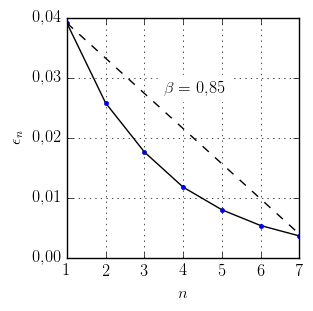
\includegraphics{./cap_equacao1d/pics/ex_ponto_fixo_3/ex_ponto_fixo_3}
  \caption{Decaimento do erro $\epsilon_n = |x^{(n)}-x^*|$ da iteração do ponto fixo estudada no Exemplo~\ref{ex:ponto_fixo_3}.}
  \label{fig:ex_ponto_fixo_3}
\end{figure}


%%%%%%%%%%%%%%%%%%%%
% scilab
%%%%%%%%%%%%%%%%%%%%
\ifisscilab
No \verb+Scilab+, podemos computar estas iterações e o erro absoluto com o seguinte código:
\begin{verbatim}
//est. da solucao
deff('y = f(x)', 'y = cos(x)-x')
xe = fsolve(0.7, f)

#funcao do pto. fixo
deff('y = g(x)', 'y = cos(x)')

#aprox. inicial
x0 = 0.7
eps = abs(x0-xe)
disp([x0, eps])

for i=2:7
  x = g(x0)
  eps = abs(x-xe)
  disp([x, eps])
  x0 = x
end
\end{verbatim}
\fi
%%%%%%%%%%%%%%%%%%%%
%%%%%%%%%%%%%%%%%%%%
% octave
%%%%%%%%%%%%%%%%%%%%
\ifisoctave
No \verb+GNU Octave+, podemos computar estas iterações e o erro absoluto com o seguinte código:
\begin{verbatim}
#est. da solucao
f = @(x) cos(x)-x;
xe = fsolve(f, 0.7);

#funcao do pto. fixo
g = @(x) cos(x);

#aprox. inicial
x0 = 0.7;
eps = abs(x0-xe);
printf("%1.5f %1.1e\n", x0, eps);

for i=2:7
  x = g(x0);
  eps = abs(x-xe);
  printf("%1.5f %1.1e\n", x, eps)
  x0 = x;
endfor
\end{verbatim}
\fi
%%%%%%%%%%%%%%%%%%%%
%%%%%%%%%%%%%%%%%%%%
% python
%%%%%%%%%%%%%%%%%%%%
\ifispython
Em \verb+Python+, podemos computar estas iterações, o erro absoluto com o seguinte código:
\begin{verbatim}
#funcao do pto. fixo
def g(x):
    return np.cos(x)

#est. da solucao
xe = sci.optimize.fixed_point(g, 0.7)

#aprox. inicial
x0 = 0.7
eps = np.fabs(x0-xe)
print("%1.5f %1.1e\n" % (x0, eps))

for i in np.arange(7):
  x = g(x0);
  eps = np.fabs(x-xe);
  print("%1.5f %1.1e\n" % (x, eps))
  x0 = x
\end{verbatim}
\fi
%%%%%%%%%%%%%%%%%%%%
\end{sol}

\subsection{Teste de convergência}
Seja $g:[a,b]\to\mathbb{R}$ uma função $C^0[a,b]$ e $x^*\in(a,b)$ um ponto fixo de $g$. Então $x^*$ é dito estável se existe uma região $(x^*-\delta,x^*+\delta)$ chamada bacia de atração tal que $x^{(n+1)}=g(x^{(n)})$ é convergente sempre que $x^{(0)}\in(x^*-\delta,x^*+\delta)$.

\begin{prop}[Teste de convergência]
 Se $g\in C^1[a,b]$ e  $|g'(x^*)|<1$, então $x^*$ é estável. Se $|g'(x^*)|>1$ é instável e o teste é inconclusivo quando $|g'(x^*)|=1$.
\end{prop}

\begin{figure}[h]
    \centering
        \includegraphics{./cap_equacao1d/pics/ponto_fixo_instavel/ponto_fixo_instavel.eps}
~
        \includegraphics{./cap_equacao1d/pics/ponto_fixo_estavel/ponto_fixo_estavel.eps}
    \caption{Ilustração das iterações do ponto fixo para: (esquerda) $y = g_1(x)$ e (direita) $y = g_2(x)$. Veja Exemplo~\ref{ex:ponto_fixo_4}.} \label{fig:teste_de_convergencia}
\end{figure}

\begin{ex}\label{ex:ponto_fixo_4}
  No Exemplo~\ref{ex:ponto_fixo_2}, observamos que a função $g_1(x)$ nos forneceu uma iteração divergente, enquanto que a função $g_2(x)$ forneceu uma iteração convergente (veja a Figura~\ref{fig:teste_de_convergencia}. Estes comportamentos são explicados pelo teste da convergência. Com efeito, sabemos que o ponto fixo destas funções está no intervalo $[1,6, 1,8]$ e temos:
  \begin{equation*}
    |g_1'(x)| = |1 - 0,5(x+1)e^x| > 4,8,\quad\forall x\in [1,6, 1,8],
  \end{equation*}
enquanto:
\begin{equation*}
  |g_2'(x)| = |1 - 0,05(x+1)e^x| < 0,962,\quad\forall x\in [1,6, 1,8].
\end{equation*}
\end{ex}

\subsection{Estabilidade e convergência}\index{iteração do ponto fixo!estabilidade}\index{iteração do ponto fixo!convergência}

A fim de compreendermos melhor os conceitos de estabilidade e convergência, considere uma função $\Phi(x)$ com um ponto fixo $x^*=g(x^*)$ e analisemos o seguinte processo iterativo:
\begin{eqnarray*}
x^{(n+1)}&=&g\left(x^{(n)}\right)\\
x^{(0)}&=&x
\end{eqnarray*}
Vamos supor que a função $g(x)$ pode ser aproximada por seu polinômio de Taylor em torno do ponto fixo:
\begin{eqnarray*}
g(x)&=&g(x^*)+(x-x^*) g'(x^*)+O\left((x-x^*)^2\right), n\geq 0\\
&=&x^*+(x-x^*) g'(x^*)+O\left((x-x^*)^2\right)\\
&\approx& x^*+(x-x^*) g'(x^*)
\end{eqnarray*}

Substituindo na relação de recorrência, temos
$$
x^{(n+1)}=g\left(x^{(n)}\right)\approx x^*+(x^{(n)}-x^*) g'(x^*)
$$
Ou seja:
$$
\left(x^{(n+1)}-x^*\right)\approx {(x^{(n)}-x^*)} g'(x^*)
$$
Tomando módulos, temos:
$$
\underbrace{\left|x^{(n+1)}-x^*\right|}_{\epsilon_{n+1}}\approx \underbrace{\left|x^{(n)}-x^*\right|}_{\epsilon_n} \left|g'(x^*)\right|,
$$
onde $\epsilon_n=\left|x^{(n)}-x^*\right|$.

\begin{obs} A análise acima, concluímos:
\begin{itemize}
\item Se $|g'(x^*)|<1$, então, a distância de $x^{(n)}$ até o ponto fixo $x^*$ está diminuindo a cada passo.
\item Se $|g'(x^*)|>1$, então, a distância de $x^{(n)}$ até o ponto fixo $x^*$ está aumentando a cada passo.
\item Se $|g'(x^*)|=1$, então, nossa aproximação de primeira ordem não é suficiente para compreender o comportamento da sequência.
\end{itemize}
\end{obs}

\subsection{Erro absoluto e tolerância}\index{erros!absoluto}\index{tolerância}

Na prática, quando se aplica uma iteração como esta, não se conhece de antemão o valor do ponto fixo $x^*$. Assim, o erro $\epsilon_n=\left|x^{(n)}-x^*\right|$ precisa ser estimado com base nos valores calculados $x^{(n)}$. Uma abordagem frequente é analisar a evolução da diferença entre dois elementos da sequência:
$$\Delta_n=\left|x^{(n+1)}-x^{(n)}\right|$$

A pergunta natural é: Será que o erro $\epsilon_n=\left|x^{(n)}-x^*\right|$ é pequeno quando  $\Delta_n=\left|x^{(n+1)}-x^{(n)}\right|$ for pequeno?

Para responder a esta pergunta, observamos que
$$x^*=\lim_{n\to \infty }x^{(n)}$$
portanto:
\begin{eqnarray*}
x^*-x^{(N)}&=&  \left(x^{(N+1)}-x^{(N)}\right)+\left(x^{(N+2)}-x^{(N+1)}\right)+\left(x^{(N+3)}-x^{(N+2)}\right)+\ldots\\
&=&\sum_{k=0}^\infty \left(x^{(N+k+1)}-x^{(N+k)}\right)
\end{eqnarray*}

Usamos também as expressões:
\begin{eqnarray*}
x^{(n+1)}&\approx& x^*+(x^{(n)}-x^*) g'(x^*)\\
x^{(n)}&\approx& x^*+(x^{(n-1)}-x^*) g'(x^*)
\end{eqnarray*}
Subtraindo uma da outra, temos:
\begin{eqnarray*}
x^{(n+1)}-x^{(n)}&\approx& (x^{(n)}-x^{(n-1)}) g'(x^*)
\end{eqnarray*}
Portanto:
\begin{eqnarray*}
x^{(N+k+1)}-x^{(N+k)}&\approx& (x^{(N+1)}-x^{(N)}) \left(g'(x^*)\right)^{k}
\end{eqnarray*}
E temos:
\begin{eqnarray*}
x^*-x^{(N)}
&=&\sum_{k=0}^\infty \left(x^{(N+k+1)}-x^{(N+k)}\right)\\
&\approx&\sum_{k=0}^\infty (x^{(N+1)}-x^{(N)}) \left(g'(x^*)\right)^{k}\\
&=&(x^{(N+1)}-x^{(N)}) \frac{1}{1-g'(x^*)}, \quad \left|g'(x^*)\right|<1
\end{eqnarray*}
Tomando módulo, temos:
\begin{eqnarray*}
\left|x^*-x^{(N)} \right|
&\approx&\left|x^{(N+1)}-x^{(N)}\right| \frac{1}{1-g'(x^*)}\\
\epsilon_N &\approx&  \frac{\Delta_N}{1-g'(x^*)}
\end{eqnarray*}

\begin{obs}
Tendo em mente a relação $x^{(n+1)}-x^{(n)}  \approx (x^{(n)}-x^{(n-1)}) g'(x^*)$, concluímos:
\begin{itemize}

\item Quando $g'(x^*)<0$, o esquema é alternante, isto é, o sinal do erro se altera a cada passo.  O erro $\epsilon_N$ pode ser estimado diretamente da diferença $\Delta_N$, pois o denominador $1-g'(x^*)>1$.
\item Quando $0<g'(x^*)<1$, o esquema é monótono e $\frac{1}{1-g'(x^*)}>1$, pelo que o erro $\epsilon_N$ é maior que a diferença $\Delta_N$. A relação será tão mais importante quando mais próximo da unidade for $g'(x^*)$, ou seja, quando mais lenta for a convergência. Para estimar o erro em função da diferença $\Delta_N$, observamos que  $g'(x^*)\approx \frac{x^{(n+1)}-x^{(n)}}{x^{(n)}-x^{(n-1)}}$ e 
$$\left|g'(x^*)\right|\approx \frac{\Delta_n}{\Delta_{n-1}}$$
e portanto
$$\epsilon_N \approx \frac{\Delta_N}{1-\frac{\Delta_n}{\Delta_{n-1}}}.$$
\end{itemize}  
\end{obs}

\subsection*{Exercícios}

\begin{exer}
  Resolver a equação $e^x = x + 2$ é equivalente a calcular os pontos fixos da função $g(x) = e^x - 2$ (veja o Exemplo~\ref{ex:ponto_fixo_1}). Use a iteração do ponto fixo $x^{(n+1)} = g(x^{n})$ com $x^{(1)} = -1,8$ para obter uma aproximação de uma das soluções da equação dada com $8$ dígitos significativos.
\end{exer}
\begin{resp}
    $-1,8414057$
\end{resp}

\begin{exer}  Mostre que a equação:
  \begin{equation*}
    \cos(x)=x  
  \end{equation*}
possui uma única solução no intervalo $[0, 1]$. Use a iteração do ponto fixo e encontre uma aproximação para esta solução com  4 dígitos significativos.
\end{exer}
\begin{resp}
  
    $0,7391$
  
\end{resp}

\begin{exer}
  Mostre que a equação $xe^x = 10$ é equivalente às seguintes equações:
\begin{equation*}
  x=\ln\left(\frac{10}{x}\right)\quad\text{e}\quad x=10e^{-x}.
\end{equation*}
Destas, considere as seguintes iterações de ponto fixo:
\begin{enumerate}
 \item [a)] $\displaystyle x^{(n+1)}=\ln \left(\frac{10}{x^{(n)}}\right)$
 \item [b)] $\displaystyle x^{(n+1)}=10 e^{-x^{(n)}} $
\end{enumerate}
Tomando $x^{(1)} = 1$, verifique se estas sequências são convergentes.
\end{exer}
\begin{resp}
  
Tomemos $x^{(1)}=1$ como aproximação inicial para a solução deste problema, iterando a primeira sequência a), obtemos:
\begin{eqnarray*}
x^{(1)} &=& 1\\
x^{(2)} &=& \ln\left(\frac{10}{1}\right)=2,3025851\\
x^{(3)} &=& \ln\left(\frac{10}{2,3025851}\right)=1,4685526\\
        &\vdots&\\
x^{(21)}&=& 1,7455151\\
x^{(31)}&=& 1,745528\\
x^{(32)}&=& 1,745528
\end{eqnarray*}

Iterando a segunda sequência b), obtemos:
\begin{eqnarray*}
x^{(1)}&=&1\\
x^{(2)}&=&10e^{-1}= 3,6787944   \\
x^{(3)}&=&10e^{- 3,6787944 }= 0,2525340     \\
x^{(4)}&=&10e^{-0,2525340}=  7,7682979      \\
x^{(5)}&=&10e^{-7,7682979}=  0,0042293      \\
x^{(6)}&=&10e^{-0,0042293}=  9,9577961
\end{eqnarray*}

Este experimento numérico sugere que a iteração a) converge para $1,745528$ e a iteração b) não é convergente.    
  
\end{resp}

\begin{exer} Verifique (analiticamente) que a única solução real da equação:
  \begin{equation*}
    xe^x=10
  \end{equation*}
é ponto fixo das seguintes funções:
\begin{itemize}
\item[a)] $g(x)=\ln\left(\frac{10}{x}\right)$
\item[b)] $g(x)=x-\frac{xe^{x}-10}{15}$
\item[c)] $g(x)=x-\frac{xe^{x}-10}{10+e^{x}}$
\end{itemize}
Implemente o processo iterativo $x^{(n+1)}=g(x^{(n)})$ para $n\geq 0$ e compare o comportamento. Discuta os resultados com base na teoria estudada.
\end{exer}

\begin{exer} Verifique (analiticamente) que a única solução real da equação:
  \begin{equation*}
    \cos(x)=x  
  \end{equation*}
é ponto fixo das seguintes funções:
\begin{itemize}
\item[a)] $g(x)=\cos(x)$
\item[b)] $g(x)=0,4 x+ 0,6\cos(x)$
\item[c)] $g(x)=x+\frac{\cos(x)-x}{1+\sin(x)}$
\end{itemize}
Implemente o processo iterativo $x^{(n+1)}=g(x^{(n)})$ para $n\geq 0$ e compare o comportamento. Discuta os resultados com base na teoria estudada.
\end{exer}


\begin{exer} Encontre a solução de cada equação com erro absoluto inferior a $10^{-6}$.
  \begin{itemize}
  \item[a)] $e^x=x+2$ no intervalo $(-2,0)$.
  \item[b)] $x^3+5x^2-12=0$ no intervalo $(1,2)$.
  \item[c)] $\sqrt{x}=\cos(x)$ no intervalo $(0,1)$.
  \end{itemize}
\end{exer}

\begin{exer} Encontre numericamente as três primeiras raízes positivas da equação dada por:
  \begin{equation*}
    \cos(x)=\frac{x}{10+x^2}  
  \end{equation*}
com erro absoluto inferior a $10^{-6}$.
\end{exer}
\begin{resp}
 $x_1\approx 1,4506619$, $x_2\approx 4,8574864$, $x_3= 7,7430681$. 
\end{resp}



\begin{exer} Considere os seguintes processos iterativos:
\begin{equation*}
\begin{array}{l}
a\left\{\begin{array}{rcl}
x^{(n+1)}&=&\cos(x^{(n)})\\
x^{(1)}&=&.5
\end{array}
\right. \\ \qquad \text { e }\\
b\left\{\begin{array}{rcl}
x^{(n+1)}&=&.4x^{(n)}+.6\cos(x^{(n)})\\
x^{(1)}&=&.5
\end{array}
\right.
\end{array}
\end{equation*}

Use o teorema do ponto fixo para verificar que cada um desses processos converge para a solução da equação $x^*$ de $\cos(x)=x$. Observe o comportamento numérico dessas sequências. Qual estabiliza mais rápido com cinco casas decimais? Discuta.

Dica: Verifique que $\cos([0.5,1])\subseteq [0.5,1]$ e depois a mesma identidade para a função $f(x)=0,4x+0,6\cos(x)$.
\end{exer}


\begin{exer}  Use o teorema do ponto fixo aplicado a um intervalo adequado para mostrar que a função $g(x)=\ln (100-x)$ possui um ponto fixo estável.
\end{exer}

\begin{exer}(Fluidos) Na hidráulica, o fator de atrito de Darcy é dado pela implicitamente pela equação de Colebrook-White:
$$\frac{1}{\sqrt{f}}= -2 \log_{10} \left( \frac{\varepsilon}{14.8 R_h} + \frac{2.51}{\mathrm{Re}\sqrt{f}} \right)$$
onde $f$ é o fator de atrito, $\varepsilon$ é a rugosidade do tubo em metros, $R_{h}$ é o raio hidráulico em metros e ${Re}$ é o número de Reynolds. Considere $\varepsilon=2mm$, $R_{h}=5cm$ e ${Re}=10000$ e obtenha o valor de $f$ pela iteração:
$$x^{(n+1)}=-2 \log_{10} \left( \frac{\varepsilon}{14.8 R_{h}} + \frac{2.51x^{(n)}}{\mathrm{Re}} \right)$$
\end{exer}
\begin{resp}
  
$0.0431266$
  
\end{resp}

\begin{exer} Encontre uma solução aproximada para equação algébrica
$$180-100x=0.052\sinh^{-1}(10^{13}x)$$
com erro absoluto inferior a $10^{-3}$ usando um método iterativo.
Estime o erro associado ao valor de $v=180-100x=0.052\sinh^{-1}(10^{13}x)$, usando cada uma dessas expressões. Discuta sucintamente o resultado obtido. Dica: Este caso é semelhante ao Problema~\ref{prob_diodo}.
\end{exer}

\begin{exer}Considere que $x_n$ satisfaz a seguinte relação de recorrência:
$$x_{n+1}=x_n - \beta \left(x_n-x^*\right)$$
onde $\beta$ e $x^*$ são constantes.
Prove que $$x_n-x^*=(1-\beta)^{n-1}(x_1-x^*).$$
Conclua que $x_n\to x^*$ quando $|1-\beta|<1$.
\end{exer}

\begin{exer}(Convergência lenta) Considere o seguinte esquema iterativo:
  \begin{eqnarray*}
    x^{(n+1)} &=& x_n+q^n,\\
    x^{(0)} &=& 0,   
  \end{eqnarray*}
onde $q=1-10^{-6}$.
\begin{itemize}
\item[a)] Calcule o limite $$x_\infty=\lim_{n\to\infty}x^{(n)}$$ analiticamente.
\item[b)] Considere que o problema de obter o limite da sequência numericamente usando como critério de parada que $|x^{(n+1)}-x^{(n)}|<10^{-5}$. Qual o valor é produzido pelo esquema numérico? Qual o desvio entre o valor obtido pelo esquema numérico e o valor do limite obtido no item a?  Discuta. (Dica: Você não deve implementar o esquema iterativo, obtendo o valor de $x^{(n)}$ analiticamente)
\item[c)] Qual deve ser a tolerância especificada para obter o resultado com erro relativo inferior a $10^{-2}$?
\end{itemize}
\end{exer}

\begin{exer}(Convergência sublinear) Considere o seguinte esquema iterativo:
$$x^{(n+1)}=x^{(n)}-[x^{(n)}]^3,\ x^{(n)}\geq 0$$
com $x^{(0)}= 10^{-2}$.
Prove que $\{x^{(n)}\}$ é sequência de número reais positivos convergindo para zero. Verifique que são necessários mais de mil passos para que $x^{(n)}$ se torne menor que $0.9 x^{(0)}$.
\end{exer}


\begin{exer}(Taxa de convergência)
\begin{itemize}
\item[a)] Use o teorema do ponto fixo para mostrar que a função $g(x)=1-\sin(x)$ possui um único ponto fixo estável o intervalo $[\frac{1}{10},1]$. Construa um método iterativo $x^{(n+1)}=g(x^{(n)})$ para encontrar esse ponto fixo. Use o computador para encontrar o valor numérico do ponto fixo.
\item[b)] Verifique que função $\psi(x)=\frac{1}{2}\left[x+1-\sin(x)\right]$ possui um ponto fixo $x^*$ que também é o ponto fixo da função $g$ do item a. Use o computador para encontrar o valor numérico do ponto fixo através da iteração $x^{(n+1)}=\psi(x^{(n)})$. Qual método é mais rápido?
\end{itemize}
\end{exer}


\begin{exer}(Esquemas oscilantes)(\textit{Esquemas oscilantes})
\begin{itemize}
\item[a)] Considere a função $g(x)$ e função composta $\psi(x)=g\circ g=g\left(g(x)\right)$. Verifique todo ponto fixo de $g$ também é ponto fixo de $\psi$.

\item[b)]  Considere a função $$g(x)=10\exp(-x)$$ e função composta $\psi(x)=g\circ g=g\left(g(x)\right)$. Mostre que $\psi$ possui dois pontos fixos que não são pontos fixos de $g$.

\item[c)]  No problema anterior, o que acontece quando o processo iterativo $x^{(n+1)}=g(x^{(n)})$ é inicializado com um ponto fixo de $\psi$ que não é ponto fixo de $g$?
\end{itemize}
\end{exer}

\begin{exer}(Aceleração de convergência - introdução ao método de Newton)\label{int_new1} Mostre que se $f(x)$ possui uma raiz $x^*$ então a $x^*$ é um ponto fixo de $\phi(x)=x+\gamma(x) f(x)$. Encontre uma condição em $\gamma(x)$ para que o ponto fixo $x^*$ de $\phi$ seja estável. Encontre uma condição em $\gamma(x)$ para que $\phi'(x^*)=0$.
\end{exer}

\begin{exer}(Aceleração de convergência - introdução ao método de Newton)\label{int_new2} Considere que $x^{(n)}$ satisfaz a seguinte relação de recorrência:
$$x^{(n+1)}=x^{(n)} - \gamma f(x^{(n)})$$
onde $\gamma$ é uma constante. Suponha que $f(x)$ possui um zero em $x^*$. Aproxime a função $f(x)$ em torno de $x^*$ por
$$f(x)=f(x^*)+f'(x^*)(x-x^*)+O\left((x-x^*)^2\right).$$
Em vista do problema anterior, qual valor de $\gamma$ você escolheria para que a sequência $x^{(n)}$ convirja rapidamente para $x^*$. 
\end{exer}

\begin{exer} Considere o problema da Questão~\ref{prob_diodo} e dois seguintes esquemas iterativos.
$$\begin{array}{l}
A\left\{
\begin{array}{ll}
I^{(n+1)}=\frac{1}{R}\left[V-v_t\ln\left(1+\frac{I^{(n)}}{I_R}\right)\right],n>0\\
I^{(0)}=0
\end{array}\right.\\ \hspace{2cm} \text{ e }\\
B\left\{
\begin{array}{ll}
I^{(n+1)}=I_R\left[\exp\left(\frac{V-RI^{(n)}}{v_t}\right)-1\right],n>0\\
I^{(0)}=0
\end{array}\right.
\end{array}
$$
Verifique numericamente que apenas o processo A é convergente para a, b e c; enquanto apenas o processo B é convergente para os outros itens.
\end{exer}

\section{Método de Newton-Raphson}\index{método de Newton-Raphson}\label{metodo_newton_1d}

Nesta seção, apresentamos o \emph{método de Newton-Raphson}\footnote{Joseph Raphson, 1648 - 1715, matemático inglês.}\footnote{Também chamado apenas de método de Newton.}\index{método de!Newton-Raphson}\index{método de!Newton} para calcular o zero de funções reais de uma variável real. 

Assumimos que $x^*$ é um zero de uma dada função $f(x)$ continuamente diferenciável, isto é, $f(x^*) = 0$. Afim de usar a iteração do ponto fixo, observamos que, equivalentemente, $x^*$ é um ponto fixo da função:
\begin{equation*}
  g(x)= x + \alpha(x)f(x),\quad\alpha(x)\neq 0,
\end{equation*}
onde $\alpha(x)$ é uma função arbitrária que queremos escolher de forma que a iteração do ponto fixo tenha ótima taxa de convergência. 

Do \emph{Teorema do ponto fixo}\index{teorema do!ponto fixo} temos que a taxa de convergência é dada em função do valor absoluto da derivada de $g(x)$. Calculando a derivada temos:
\begin{equation*}
  g'(x)=1+\alpha(x)f'(x)+\alpha'(x)f(x).
\end{equation*}
No ponto $x = x^*$, temos:
\begin{equation*}
  g'(x^*) = 1 + \alpha(x^*)f'(x^*) + \alpha'(x^*)f(x^*).
\end{equation*}
Como $f(x^*)=0$, temos:
\begin{equation*}
  g'(x^*) = 1 + \alpha(x^*)f'(x^*).
\end{equation*}

Sabemos que o processo iterativo converge tão mais rápido quanto menor for $|g'(x)|$ nas vizinhanças de $x^*$. Isto nos leva a escolher:
\begin{equation*}
  g'(x^*) = 0,
\end{equation*}
e, então, temos:
\begin{equation*}
  \alpha(x^*) = -\frac{1}{f'(x^*)},
\end{equation*}
se $f'(x^*)\neq 0$.

A discussão acima nos motiva a introduzir o método de Newton, cujas iterações são dada por:
\begin{equation*}
  x^{(n+1)} = x^{(n)} - \frac{f\left(x^{(n)}\right)}{f'\left(x^{n}\right)}, \quad n\geq 1,
\end{equation*}
sendo $x^{(1)}$ uma aproximação inicial dada.

\subsection{Interpretação geométrica}

Seja dada uma função $f(x)$ conforme na Figura~\ref{fig:metodo_de_Newton}. Para tanto, escolhemos uma aproximação inicial $x^{(1)}$ e computamos:
\begin{equation*}
  x^{(2)} = x^{(1)} - \frac{f(x^{(1)})}{f'(x^{(1)})}.
\end{equation*}
Geometricamente, o ponto $x^{(2)}$ é a interseção da reta tangente ao gráfico da função $f(x)$ no ponto $x = x^{(1)}$ com o eixo das abscissas. Com efeito, a equação desta reta é:
\begin{equation*}
  y = f'(x^{(1)})(x - x^{(1)}) + f(x^{(1)}).
\end{equation*}
Assim, a interseção desta reta com o eixo das abscissas ocorre quando ($y=0$):
\begin{equation*}
  f'(x^{(1)})(x - x^{(1)}) + f(x^{(1)}) = 0\Rightarrow x = x^{(1)} - \frac{f(x^{(1)})}{f'(x^{(1)})}.
\end{equation*}

\begin{figure}[h]
  \centering
  \includegraphics{./cap_equacao1d/pics/metodo_de_Newton/metodo_de_Newton.eps}  
  \caption{Interpretação do método de Newton.}
  \label{fig:metodo_de_Newton}
\end{figure}

Ou seja, dado $x^{(n)}$ a próxima aproximação $x^{(n+1)}$ é o ponto de interseção entre o eixo das abscissas e a reta tangente ao gráfico da função no ponto $x = x^{(n)}$. Observe a Figura~\ref{fig:metodo_de_Newton}.

\subsection{Análise de convergência}\index{método de Newton-Raphson!convergência}\label{Analise_conv_Newton}

Seja $f(x)$ um função com derivadas primeira e segunda contínuas tal que $f(x^*)=0$ e $f'(x^*)\neq 0$. Seja também a função $g(x)$ definida como:
\begin{equation*}
  g(x)=x-\frac{f(x)}{f'(x)}.
\end{equation*}
Expandimos em série de Taylor em torno de $x = x^*$, obtemos:
\begin{equation*}
  g(x)=g(x^*)+g'(x^*)(x-x^*) + \frac{g''(x^*)}{2}(x-x^*)^2 + O\left((x-x^*)^3\right).
\end{equation*}
Observamos que:
\begin{eqnarray*}
g(x^*) &=& x^*\\
g'(x^*) &=& 1 - \frac{f'(x^*)f'(x^*)-f(x^*)f''(x^*)}{\left(f'(x^*)\right)^2} = 0
\end{eqnarray*}
Portanto:
\begin{equation*}
g(x) = x^* + \frac{g''(x^*)}{2}(x-x^*)^2 + O\left((x-x^*)^3\right)\\
\end{equation*}
Com isso, temos:
\begin{equation*}
x^{(n+1)} = g(x^{(n)}) =  x^*+ \frac{g''(x^*)}{2}(x^{(n)}-x^*)^2 + O\left((x-x^*)^3\right),
\end{equation*}
ou seja:
\begin{equation*}
\left|x^{(n+1)}-x^*\right| \leq C\left|x^{(n)}-x^*\right|^2,
\end{equation*}
com constante $C = \left|g''(x^*)/2\right|$. Isto mostra que o método de Newton tem \emph{taxa de convergência quadrática}. Mais precisamente, temos o seguinte teorema.

\begin{teo}[Método de Newton]
  Sejam $f\in C^2([a, b])$ com $x^*\in (a, b)$ tal que $f(x^*) = 0$ e:
  \begin{equation*}
    m := \min_{x\in [a, b]}|f'(x)| > 0\quad\text{e}\quad M := \max_{x\in [a, b]} |f''(x)|.
  \end{equation*}
Escolhendo $\rho > 0$ tal que:
\begin{equation*}
  q := \frac{M}{2m}\rho < 1, 
\end{equation*}
definimos a \emph{bacia de atração} do método de Newton pelo conjunto:
\begin{equation*}
  K_\rho(x^*) := \left\{x\in\mathbb{R};~|x-x^*| \leq \rho\right\}\subset [a, b].
\end{equation*}
Então, para qualquer $x^{(1)}\in K_\rho(x^*)$ a iteração do método de Newton:
\begin{equation*}
  x^{(n+1)} = x^{(n)} - \frac{f(x^{(n)})}{f'(x^{(n)})},
\end{equation*}
fornece uma sequência $x^{(n)}$ que converge para $x^*$, isto é, $x^{(n)}\to x^*$ quando $n\to \infty$. Além disso, temos a seguinte estimativa de erro \emph{a priori}:
\begin{equation*}
  |x^{(n)} - x^*| \leq \frac{2m}{M}q^{(2^{n-1})},\quad n\geq 2,
\end{equation*}
e a seguinte estimativa de erro \emph{a posteriori}:
\begin{equation*}
  |x^{(n)} - x^*| \leq \frac{M}{2m}|x^{(n)} - x^{(n-1)}|^2,\quad n\geq 2.
\end{equation*}
\end{teo}
\begin{proof}
  Para $n\in\mathbb{N}$, $n\geq 2$, temos:
  \begin{equation}\label{eq:forma}
    x^{n+1}-x^* = x^{(n)} - \frac{f(x^{(n)})}{f'(x^{(n)})} - x^* = -\frac{1}{f(x^{(n)})}\left[f(x^{(n)})+(x^*-x^{(n)})f'(x^{(n)}\right].
  \end{equation}
Agora, para estimar o lado direito desta equação, usamos o polinômio de Taylor de grau $1$ da função $f(x)$ em torno de $x = x^{(n)}$, isto é:
\begin{equation*}
  f(x^*) = f(x^{(n)}) + (x^* - x^{(n)})f'(x^{(n)}) + \int_{x^{(n)}}^{x^*} f''(t)(x^* - t)\,dt.
\end{equation*}
Pela mudança de variável $t = x^{(n)} + s(x^{(n)} - x^*)$, observamos que o resto deste polinômio de Taylor na forma integral é igual a:
\begin{equation*}
  R(x^*,x^{(n)}) := (x^* - x^{(n)})^2\int_0^1 f''\left(x^{(n)} + s(x^* - x^{(n)})\right)(1-s)\,ds.
\end{equation*}
Assim, da cota da segunda derivada de $f(x)$, temos:
\begin{equation}\label{eq:est-resto}
  |R(x^*,x^{(n)})| \leq M|x^*-x^{(n)}|^2\int_0^1 (1-s)\,ds = \frac{M}{2}|x^* - x^{(n)}|^2.
\end{equation}\label{eq:quadratica}
Se $x^{(n)}\in K_\rho(x^*)$, então de \eqref{eq:forma} e \eqref{eq:est-resto} temos:
\begin{equation}
  |x^{(n+1)} - x^*| \leq \frac{M}{2m}|x^{(n)} - x^*|^2 \leq \frac{M}{2m}\rho^2 < \rho.
\end{equation}
Isto mostra que se $x^{(n)}\in K_\rho(x^*)$, então $x^{(n+1)}\in K_\rho(x^*)$, isto é, $x^{(n)}\in K_\rho(x^*)$ para todo $n\in\mathbb{R}$.

Agora, obtemos a estimativa \emph{a priori} de \eqref{eq:quadratica}, pois:
\begin{equation*}
  |x^{(n)} - x^*| \leq \frac{2m}{M}\left(\frac{M}{2m}|x^{(n-1)}-x^*|\right)^2 \leq \cdots \leq \frac{2m}{M}\left(\frac{M}{2m} |x^{(1)}-x^*|\right)^{2^{n-1}}.
\end{equation*}
Logo:
\begin{equation*}
  |x^{(n)} - x^*| \leq \frac{2m}{M}q^{2^{n-1}},
\end{equation*}
donde também vemos que $x^{(n)}\to x^*$ quando $n\to\infty$, pois $q < 1$.

Por fim, para provarmos a estimativa \emph{a posteriori} tomamos a seguinte expansão em polinômio de Taylor:
\begin{equation*}
  f(x^{(n)}) = f(x^{(n-1)}) + (x^{(n)} - x^{(n-1)})f'(x^{(n-1)}) + R(x^{(n)},x^{(n-1)}).
\end{equation*}
Aqui, temos:
\begin{equation*}
  f(x^{(n-1)}) + (x^{(n)} - x^{(n-1)})f'(x^{(n-1)}) = 0
\end{equation*}
e, então, conforme acima:
\begin{equation*}
  |f(x^{(n)})| = |R(x^{(n)}),x^{(n-1)}| \leq \frac{M}{2}|x^{(n)} - x^{(n-1)}|^2.
\end{equation*}
Com isso e do teorema do valor médio, concluímos:
\begin{equation*}
  |x^{(n)} - x^*| \leq \frac{1}{m}|f(x^{(n)}) - f(x^*)| \leq \frac{M}{2m}|x^{(n)} - x^{(n-1)}|^2.
\end{equation*}
\end{proof}

\begin{ex}
  Estime o raio $\rho$ da bacia de atração $K_\rho(x^*)$ para a função $f(x) = \cos(x) - x$ restrita ao intervalo $[0, \pi/2]$.
\end{ex}
\begin{sol}
  O raio da bacia de atração é tal que:
  \begin{equation*}
    \rho < \frac{2m}{M}
  \end{equation*}
onde $m := \min |f'(x)|$ e $M := \max |f''(x)|$ com o mínimo e o máximo tomados em um intervalo $[a, b]$ que contenha o zero da função $f(x)$. Aqui, por exemplo, podemos tomar $[a, b] = [0, \pi/2]$. Como, neste caso, $f'(x) = -\sin(x) - 1$, temos que $m = 1$. Também, como $f''(x) = -\cos x$, temos $M = 1$. Assim, concluímos que $\rho < 2$ (lembrando que $K_\rho(x^*)\subset [0, \pi/2]$). Ou seja, neste caso as iterações de Newton convergem para o zero de $f(x)$ para qualquer escolha da aproximação inicial $x^{(1)}\in [0, \pi/2]$.
\end{sol}

\subsection*{Exercícios}

\begin{exer}\label{1d:cosx2}
Encontre a raiz positiva da função $f(x)=\cos(x)-x^2$ pelo método de Newton inicializando-o com $x^{(0)}=1$. Realize a iteração até obter estabilidade no $quinto$ dígito significativo.
\end{exer}
\begin{resp}
  raiz:0,82413, processo iterativo: $x^{(n+1)}= x^{(n)}+ \frac{\cos(x)-x^2}{\sin(x)+2x}$
  
%%%%%%%%%%%%%%%%%%%%
% scilab
%%%%%%%%%%%%%%%%%%%
\ifisscilab
\begin{verbatim}
-->x=1
-->x=x+(cos(x)-x^2)/(sin(x)+2*x)
-->x=x+(cos(x)-x^2)/(sin(x)+2*x)
-->x=x+(cos(x)-x^2)/(sin(x)+2*x)
-->x=x+(cos(x)-x^2)/(sin(x)+2*x)
\end{verbatim}
\fi
%%%%%%%%%%%%%%%%%%%%
%%%%%%%%%%%%%%%%%%%%
% octave
%%%%%%%%%%%%%%%%%%%
\ifisoctave
\begin{verbatim}
>> x=1
>> x=x+(cos(x)-x^2)/(sin(x)+2*x)
>> x=x+(cos(x)-x^2)/(sin(x)+2*x)
>> x=x+(cos(x)-x^2)/(sin(x)+2*x)
>> x=x+(cos(x)-x^2)/(sin(x)+2*x)
\end{verbatim}
\fi
%%%%%%%%%%%%%%%%%%%%
\end{resp}

\begin{exer} Considere o problema de calcular as soluções positivas da equação:
  \begin{equation*}
    \tg(x)=2x^2.    
  \end{equation*}
\begin{itemize}
\item[a)] Use o método gráfico para isolar as duas primeiras raízes positivas em pequenos intervalos. Use a teoria para argumentar quanto à existência e unicidade das raízes dentro intervalos escolhidos.
% \item[b)] Calcule o número de iterações necessárias para que o método da bisseção aproxime cada uma das raízes com erro absoluto inferior a $10^{-8}$. Calcule as raízes por este método usando este número de passos.
\item[b)]  Calcule cada uma das raízes pelo método de Newton com oito dígitos significativos e discuta a convergência comparando com o item b).
\end{itemize}
%{\bf Obs:} Alguns alunos encontraram como solução $x_1\approx 1,5707963$ e $x_2 \approx 4,7123890$. O que eles fizeram de errado?
\end{exer}
%%%%%%%%%%%%%%%%%%%%
% scilab
%%%%%%%%%%%%%%%%%%%%
\ifisscilab
\begin{resp}
  \begin{itemize}
\item[a)]Primeiramente, deve-se observar que a função $\tg(x)$ não está definida quando $x$ é um múltiplo ímpar de $\frac{\pi}{2}$, pelo que devemos cuidado nas singularidades. Traçamos o gráfico da função $f(x)=\tg(x)-2x^2$ no \verb+Scilab+ usando os seguintes comandos:
\begin{verbatim}
-->deff('y=f(x)','y=tan(x)-2*x^2')
-->plot([0:.01:1.3],f)
\end{verbatim} 
Observamos facilmente uma raiz no intervalo $(0,5, 0,6)$ e outra no intervalo $(1,2, 1,3)$. Como a função $f(x)$ é contínua fora dos pontos de singularidade da tangente, é fácil verificar que existe pelo menos uma solução nos intervalos dados pelo teorema de Bolzano~\ref{teo:teorema_de_Bolzano}:
\begin{eqnarray*}
f(0,5) &\approx& 0,046302 >0\\
f(0,6) &\approx& -0,035863 <0\\
f(1,2) &\approx& -0,30784e-1 <0\\
f(1,3) &\approx&  0,22210e-1>0\\
\end{eqnarray*} 
Para provar a unicidade da solução em cada intervalo, precisamos mostra que a função é monótona, ou seja, a derivada não muda de sinal em cada intervalo:
\begin{eqnarray*}
f'(x)=\sec^2(x)-4x=\frac{1}{\cos^2(x)}-4x\leq \frac{1}{\cos^2(0,6)}-4*0,5<0, ~~x\in[ 0,5, 0,6]\\
f'(x)=\sec^2(x)-4x=\frac{1}{\cos^2(x)}-4x\geq \frac{1}{\cos^2(1,2)}-4*1,3>0, ~~x\in[ 1,2, 1,3]\\
\end{eqnarray*} 

% \item[b)] 
% Já isolamos as raízes em intervalos de comprimento $10^{-1}$ e a precisão requerida exige que as isolemos em intervalos de comprimento $2\times 10^{-8}$. Como cada passo da bisseção, confina a raiz em um intervalo com comprimento igual à metade do comprimento do intervalo anterior, temos a seguinte condição para o número de passos $N_p$:
% $$\frac{10^{-1}}{2^N_p}\leq 2\times 10^{-8}$$
% isso é equivalente a
% $$N_p\geq \log_2 \frac{10^{-1}}{2\times 10^{-8}}=\log_2 \frac{10^{7}}{2}=7\log_2 10 -1=\frac{7}{\log_10 2}-1\approx 22.22$$
% Como $N_p$ é inteiro, o menor $N_p$ que satisfaz a condição é $23$.

% As raízes obtidas são $0.55970415$ e $1.2703426$. 

\item[b)] Para recalcular as raízes pelo método de Newton, basta executar a interação
$$x^{(n+1)}=x^{(n)}-\frac{f(x^{(n)})}{f'(x^{(n)}}$$    
\end{itemize}
Em relação à observação, o erro se deveu à falta de cuidado em compreender o problema antes de tentar resolvê-lo, em especial, à falta de observar que a função é descontínua em  múltiplos ímpares de $\frac{\pi}{2}$. Nestes pontos, a função $f(x)$ troca de sinal, mas não passa por zero.    
\end{resp}
\fi
%%%%%%%%%%%%%%%%%%%%


\begin{exer}\label{new1} Considere a equação
  $$e^{-x^2}=x$$
trace o gráfico com auxílio do computador e verifique que ela possui uma raiz positiva. Encontre uma aproximação para esta razão pelo gráfico e use este valor para inicializar o método de Newton e obtenha uma aproximação para a raiz com 8 dígitos significativos. \ifisscilab (Use o comando \verb+format('v',16)+ para alterar a visualização no \verb+Scilab+.)\fi
\end{exer}
\begin{resp}
  0,65291864    
  \end{resp}

\begin{exer}\label{new2} Isole e encontre as cinco primeiras raízes positivas da equação com 6 dígitos corretos através de traçado de gráfico e do método de Newton.
$$\cos(10x)=e^{-x}.$$ Dica: a primeira raiz positiva está no intervalo $(0, 0,02)$. Fique atento.
\end{exer}
\begin{resp}
   $0,0198679$; $0,533890$; $0,735412$; $1,13237$ e $1,38851$.
  \end{resp}


\begin{exer}\label{new3} Encontre as raízes do polinômio $f(x)=x^4-4x^2+4$ através do método de Newton. O que você observa em relação ao erro obtido? Compare com a situação do Problema~\ref{prob_raiz_dupla}.
\end{exer}

\begin{exer}\label{new4} Encontre as raízes reais do polinômio $f(x)=\frac{x^5}{100}+x^4+3x+1$ isolando-as pelo método do gráfico e depois usando o método de Newton. Expresse a solução com 7 dígitos significativos.
\end{exer}
\begin{resp}
 $-99.99970$, $-0.3376513$; $-1.314006$.
 \end{resp}

\begin{exer}Considere o método de Newton aplicado para encontrar a raiz de $f(x)=x^3-2x+2$. O que acontece quando $x^{(0)}=0$? Escolha um valor adequado para inicializar o método e obter a única raiz real desta equação.
\end{exer}

\begin{exer} Justifique a construção do processo iterativo do método de Newton através do conceito de estabilidade de ponto fixo e convergência do método da iteração. Dica: Considere os problemas \ref{int_new1} e \ref{int_new2}.
\end{exer}

\begin{exer} Entenda a interpretação geométrica ao método de Newton. Encontre uma valor para iniciar o método de Newton aplicado ao problema $f(x)=xe^{-x}=0$ tal que o esquema iterativo divirja.
\end{exer}
\begin{resp}
  
$x_0>1$.    
  
\end{resp}

\begin{exer}(Computação) Aplique o método de Newton à função $f(x)=\frac{1}{x}-A$ e construa um esquema computacional para calcular a inversa de $A$ com base em operações de multiplicação e soma/subtração.
 \end{exer}
\begin{resp}
  \begin{eqnarray*}
 x^{(0)} &=& \text{C.I.}\\
 x^{(n+1)}&=&x^{(n)}\left(2-Ax^{(n)}\right) \\ 
 \end{eqnarray*}
\end{resp}


\begin{exer}(Computação) Aplique o método de Newton à função $f(x)=x^n-A$ e construa um esquema computacional para calcular  $\sqrt[n]{A}$ para $A>0$ com base em operações de multiplicação e soma/subtração.
\end{exer}
\begin{resp}
 \begin{eqnarray*}
 x_{0} &=& \text{C.I.}\\
 x^{(n+1)}&=&x^{(n)}\left(1-\frac{1}{n}\right) + \frac{A}{n x^{(n)}}
 \end{eqnarray*}

\end{resp}


\begin{exer}(Computação) Aplique o método de Newton à função $f(x)=\frac{1}{x^2}-A$ e construa um esquema computacional para calcular  $\frac{1}{\sqrt{A}}$ para $A>0$ com base em operações de multiplicação e soma/subtração.
\end{exer}
\begin{resp}
 \begin{eqnarray*}
 x_{0} &=& \text{C.I.}\\
 x^{(n+1)}&=&x^{(n)} + \frac{x^{(n)}-Ax^{(n)}}{2}=\frac{(3-A)x^{(n)}}{2}\\ 
 \end{eqnarray*}

\end{resp}




\begin{exer} Considere a função dada por
\begin{eqnarray*}
\psi(x)&=&\ln\left(15-\ln(x)\right)
\end{eqnarray*}
definida para $x\in \left(0,e^{15}\right)$
\begin{itemize}
\item [a)] (1.5) Use o teorema do ponto fixo para provar que se $x^{(0)}$ pertence ao intervalo $[1,3]$, então a sequência dada iterativamente por $$x^{(n+1)}=\psi(x^{(n)}),n\geq 0$$ converge para o único ponto fixo, $x^*$, de $\psi$. Construa a iteração $x^{(n+1)}=\psi(x^{(n)})$ e obtenha numericamente o valor do ponto fixo $x^*$. Expresse a resposta com 5 algarismos significativos corretos.
\item [b)] (1.0) Construa a iteração do método de Newton para encontrar $x^*$, explicitando a relação de recorrência e iniciando com $x_0=2$. Use o computador para obter a raiz e expresse a resposta com oito dígitos significativos corretos.
\end{itemize}
\end{exer}

\section{Método das secantes}\index{método das secantes}

O \emph{método das secantes} é uma variação do método de Newton, evitando a necessidade de conhecer-se a derivada analítica de $f(x)$. Dada uma função $f(x)$, a ideia é aproximar sua derivada pela razão fundamental:
\begin{equation*}
  f'(x)\approx \frac{f(x)-f(x_0)}{x-x_0},\quad x\approx x_0.
\end{equation*}

Mais precisamente, o método de Newton é uma iteração de ponto fixo da forma:
\begin{equation*}
  x^{(n+1)} = x^{(n)} - \alpha(x^{(n)})f(x^{(n)}),\quad n\geq 1,
\end{equation*}
onde $x^{(1)}$ é uma aproximação inicial dada e $\alpha(x^{(n)}) = 1/f'(x^{(n)})$. Usando a aproximação da derivada acima, com $x = x^{(n)}$ e $x_0 = x^{(n-1)}$, temos:
\begin{equation*}
  \alpha(x^{(n)}) = \frac{1}{f'(x^{(n)})} \approx  \frac{x^{(n)} - x^{(n-1)}}{f(x^{(n)}) - f(x^{(n-1)})}.
\end{equation*}
Isto nos motiva a introduzir a \emph{iteração do método das secantes} dada por:
\begin{equation*}
  x^{(n+1)} = x^{(n)} - f(x^{(n)})\frac{x^{(n)} - x^{(n-1)}}{f(x^{(n)}) - f(x^{(n-1)})},\quad n\geq 2.
\end{equation*}
Observe que para inicializarmos a iteração acima precisamos de duas aproximações iniciais, a saber, $x^{(1)}$ e $x^{(2)}$. Maneiras apropriadas de escolher estas aproximações podem ser inferidas da interpretação geométrica do método.

\begin{ex} Encontre as raízes de $f(x)=\cos(x)-x$.
\end{ex}
\begin{sol}
Da inspeção do gráfico das funções $y=\cos(x)$ e $y=x$, sabemos que esta equação possui uma raiz em torno de $x=0,8$. Iniciamos o método com $x_0=0,7$ e $x_1=0,8$.
\begin{center}
\begin{tabular}{|c|c|c|c|}\hline
$x^{(n-1)}$ & $x^{(n)}$ & $m$ & $x^{(n+1)}$\\\hline
 & & $\frac{f(0,8)-f(0,7)}{0,8-0,7} =$ & $0,8- \frac{f(0,8)}{-1,6813548}=$\\
$0,7$ & $0,8$ & $-1,6813548$ & $0,7385654$\\\hline
$0,8$ & $0,7385654$ & $-1,6955107$ & $0,7390784$ \\\hline
 $0,7385654$ & $0,7390784$ &  $-1,6734174$ & $0,7390851$ \\\hline
$0,7390784$ & $0,7390851$ & $-1,6736095$ & $0,7390851$ \\\hline
\end{tabular}  
\end{center}  
\end{sol}

\subsection{Interpretação geométrica}

Enquanto, o método de Newton está relacionado às retas tangentes ao gráfico da função objetivo $f(x)$, o método das secantes, como o próprio nome indica, está relacionado às retas secantes.

\begin{figure}[h]
  \centering
  \includegraphics{./cap_equacao1d/pics/metodo_das_secantes/metodo_das_secantes.eps}
  \caption{Método das secantes.}
  \label{fig:metodo_das_secantes}
\end{figure}

Sejam $f(x)$ e as aproximações $x^{(1)}$ e $x^{(2)}$ do zero $x^*$ desta função (veja Figura~\ref{fig:metodo_das_secantes}). A iteração do método das secantes fornece:
\begin{equation*}
  x^{(3)} = x^{(2)} - f(x^{(2)})\frac{x^{(2)} - x^{(1)}}{f(x^{(2)}) - f(x^{(1)})}.
\end{equation*}
De fato, $x^{(3)}$ é o ponto de interseção da reta secante ao gráfico de $f(x)$ pelos pontos $x^{(1)}$ e $x^{(2)}$ com o eixo das abscissas. Com efeito, a equação desta reta secante é:
\begin{equation*}
  y = \frac{f(x^{(2)}) - f(x^{(1)})}{x^{(2)} - x^{(1)}}(x - x^{(2)}) + f(x^{(2)}).
\end{equation*}
Esta reta intercepta o eixo das abscissas no ponto $x$ tal que $y=0$, isto é:
\begin{equation*}
  \frac{f(x^{(2)}) - f(x^{(1)})}{x^{(2)} - x^{(1)}}(x - x^{(2)}) + f(x^{(2)}) \Rightarrow x = x^{(2)} - f(x^{(2)})\frac{x^{(2)} - x^{(1)}}{f(x^{(2)}) - f(x^{(1)})}.
\end{equation*}


\subsection{Análise de convergência}\index{método das secantes!convergência}

Uma análise assintótica semelhante àquela feita para o método de Newton na subseção~\ref{Analise_conv_Newton} nos indica que, para uma função $f(x)$ duas vezes diferenciável, as iterações do método da secante satisfazem:
\begin{equation*}
  |x^{(n+1)} - x^*| \approx C |x^{(n)} - x^*||x^{(n-1)} - x^*|,
\end{equation*}
para aproximações iniciais suficientemente próximas de $x^*$, onde $f(x^*) = 0$. Além disso, veremos que:
\begin{equation*}
  |x^{(n+1)} - x^*| \leq C |x^{(n)} - x^*|^{p},~~ p=\frac{\sqrt{5}+1}{2}\approx 1,618
\end{equation*}
sob certas condições. Ou seja, o método das secantes tem \emph{taxa de convergência superlinear}.

\begin{teo}[Método das secantes]\label{teo:metodo_das_secantes}
  Seja $f\in C^2([a, b])$ uma função com $x^*\in (a, b)$ tal que $f(x^*) = 0$. Sejam, também:
  \begin{equation*}
    m := \min_{x\in [a, b]} |f'(x)| > 0\quad\text{e}\quad M := \max_{x\in [a,b]} |f''(x)| < \infty.
  \end{equation*}
Além disso, seja $\rho > 0$ tal que:
\begin{equation*}
  q := \frac{M}{2m}\rho < 1,\quad K_\rho(x^*) := \{x\in\mathbb{R};~|x-x^*|\leq \rho\}\subset [a, b].
\end{equation*}
Então, para aproximações iniciais $x^{(1)}, x^{(2)}\in K_\rho(x^*)$, com $x^{(1)}\neq x^{(2)}$, temos que as iterações do método das secantes $x^{(n)}\in K_\rho(x^*)$, $n\geq 1$, e $x^{(n)}\to x^*$, quando $n\to\infty$. Além disso, vale a seguinte estimativa de convergência \emph{a priori}:
\begin{equation*}
  |x^{(n)} - x^*| \leq \frac{2m}{M}q^{\gamma_{n-1}},\quad n\geq 1,
\end{equation*}
onde $\{\gamma_n\}_{n\in\mathbb{N}}$ é a sequência de Fibonacci\footnote{Leonardo Fibonacci, c. 1170 - c. 1250, matemático italiano.}\footnote{A sequência de Fibonacci $\{\gamma_n\}_{n\in\mathbb{N}}$ é definida por $\gamma_0 = \gamma_1 = 1$ e $\gamma_{n+1} = \gamma_{n} - \gamma_{n-1}$, $n\geq 1$.}, bem como vale a estimativa \emph{a posteriori}:
\begin{equation*}
  |x^{(n)} - x^*| \leq \frac{M}{2m}|x^{(n)}-x^{(n-1)}||x^{(n-1)}-x^{(n-2)}|,\quad n\geq 3.
\end{equation*}
\end{teo}
\begin{proof}
  Sejam $n\in\mathbb{N}$ com $n\geq 2$ e $x^{(n)}, x^{(n-1)}\in K_\rho(x^*)$, tal que $x^{(n)}\neq x^{(n-1)}$, $x^{(n)}\neq x^*$ e $x^{(n-1)}\neq x^*$. Seja, também:
  \begin{equation*}
    g(x^{(n)},x^{(n-1)}) := x^{(n)} - f(x^{(n)})\frac{x^{(n)} - x^{(n-1)}}{f(x^{(n)}) - f(x^{(n-1)})}.
  \end{equation*}
Com isso, temos:
  \begin{eqnarray*}
    &&g(x^{(n)},x^{(n-1)}) - x^* = x^{(n)} - f(x^{(n)})\frac{x^{(n)} - x^{(n-1)}}{f(x^{(n)}) - f(x^{(n-1)})} - x^*\\
    &=& \frac{x^{(n)} - x^{(n-1)}}{f(x^{(n)}) - f(x^{(n-1)})}\left\{(x^{(n)} - x^*)\frac{f(x^{(n)}) - f(x^{(n-1)})}{x^{(n)} - x^{(n-1)}} - f(x^{(n)}) + f(x^*)\right\}.\\
  \end{eqnarray*}
Então, da cota assumida para primeira derivada de $f(x)$ e do teorema do valor médio, temos: 
\begin{equation}\label{eq:secantes-est0}
  |g(x^{(n)},x^{(n-1)}) - x^*| \leq \frac{|x^{(n)} - x^*|}{m}\left|\frac{f(x^{(n)}) - f(x^{(n-1)})}{x^{(n)} - x^{(n-1)}} - \frac{f(x^{(n)}) - f(x^*)}{x^{(n)} - x^*}\right|.
\end{equation}
Agora, iremos estimar este último termo a direita. Para tanto, começamos observando que da expansão em polinômio de Taylor de ordem $0$ da função $f(x)$ com resto na forma integral, temos:
\begin{eqnarray*}
  \frac{f(x^{(n)}) - f(x^{(n-1)})}{x^{(n)} - x^{(n-1)}} &= -\int_0^1 \frac{d}{dr}f(x^{(n)} + r(x^{(n-1)} - x^{(n)}))\frac{dr}{x^{(n)} - x^{(n-1)}}\\
  &= \int_0^1 f'(x^{(n)} + r(x^{(n-1)} - x^{(n)}))\,dr
\end{eqnarray*}
De forma análoga, temos:
\begin{equation*}
  \frac{f(x^{(n)}) - f(x^*)}{x^{(n)} - x^*} = \int_0^1 f'(x^{(n)} + r(x^* - x^{(n)}))\,dr
\end{equation*}
Logo, temos:
\begin{equation}\label{eq:secantes-0}
  \begin{split}
  &\frac{f(x^{(n)}) - f(x^{(n-1)})}{x^{(n)} - x^{(n-1)}} - \frac{f(x^{(n)}) - f(x^*)}{x^{(n)} - x^*} = \\
  &\int_0^1 \left[f'(x^{(n)} + r(x^{(n-1)} - x^{(n)})) - f'(x^{(n)} + r(x^* - x^{(n)}))\right]\,dr.    
  \end{split}
\end{equation}
Agora, novamente temos:
\begin{equation*}
  \begin{split}
  &f'(x^{(n)} + r(x^{(n-1)} - x^{(n)})) - f'(x^{(n)} + r(x^* - x^{(n)}))\\
  &= \int_0^r \frac{d}{ds}f'(x^{(n)} + r(x^{(n-1)} - x^{(n)}) + s(x^* - x^{(n-1)}))\,ds\\
  &= \int_0^r f''(x^{(n)} + r(x^{(n-1)} - x^{(n)}) + s(x^* - x^{(n-1)}))\,ds(x^* - x^{(n-1)}).
  \end{split}
\end{equation*}
Retornando à Equação~\eqref{eq:secantes-0} e usando a cota para a segunda derivada, obtemos:
\begin{equation*}
  \left|\frac{f(x^{(n)}) - f(x^{(n-1)})}{x^{(n)} - x^{(n-1)}} - \frac{f(x^{(n)}) - f(x^*)}{x^{(n)} - x^*} \right| \leq \frac{M}{2}|x^{(n-1)} - x^*|.
\end{equation*}
Utilizando a Equação~\eqref{eq:secantes-est0}, obtemos:
\begin{equation*}
  |g(x^{(n)},x^{(n-1)})-x^*| \leq \frac{M}{2m}|x^{(n)}-x^*||x^{(n-1)}-x^*| \leq \frac{M}{2m}\rho^2 < \rho.
\end{equation*}
Portanto, concluímos que as iterações do método da secantes $x^{(n)}$ permanecem no conjunto $K_\rho(x^*)$, se começarem nele. Além disso, temos demonstrado que:
\begin{equation*}
  |x^{(n+1)} - x^*| \leq \frac{M}{2m}|x^{(n)} - x^*||x^{(n-1)} - x^*|.
\end{equation*}
Com isso, temos:
\begin{equation*}
  \rho_n := \frac{M}{2m}|x^{(n)} - x^*| \Rightarrow \rho_{n+1} \leq \rho_{n}\rho_{n-1},\quad n\geq 2.
\end{equation*}
Como $\rho_1 \leq q$ e $\rho_2 \leq q$, temos $\rho_n \leq q^{\gamma_{n-1}}$, $n\geq 1$. Isto mostra a estimativa de convergência \emph{a priori}:
\begin{equation*}
  |x^{n} - x^*| \leq \frac{2m}{M}q^{\gamma_{n-1}}.
\end{equation*}
Além disso, como $\gamma_{n}\to \infty$ quando $n\to\infty$ e $q < 1$, temos que as iterações do método das secantes $x^{(n)}\to x^*$ quando $n\to \infty$.

Por fim, mostramos a estimativa de convergência \emph{a posteriori}. Para tanto, da cota assumida para a primeira derivada e do teorema do valor médio, temos, para $n\geq 3$:
\begin{eqnarray*}
  |x^{(n)} - x^*| &\leq& \frac{1}{m}|f(x^{(n)} - f(x^*)|\\
  &=& \frac{1}{m}\left|f(x^{(n-1)}) + (x^{(n)} - x^{(n-1)})\frac{f(x^{(n)}) - f(x^{(n-1)})}{x^{(n)} - x^{(n-1)}}\right|\\
  &=& \frac{1}{m}\left|x^{(n)} - x^{(n-1)}\right|\left|\frac{f(x^{(n)}) - f(x^{(n-1)})}{x^{(n)} - x^{(n-1)}} + \frac{f(x^{(n-1)})}{x^{(n)} - x^{(n-1)}}\right|.
\end{eqnarray*}
Agora, a iteração do método das secantes fornece:
\begin{equation*}
  x^{(n)} = x^{(n-1)} - f(x^{(n-1)})\frac{x^{(n-1)} - x^{(n-2)}}{f(x^{(n-1)}) - f(x^{(n-2)})} 
\end{equation*}
e temos:
\begin{equation*}
  \frac{f(x^{(n-1)})}{x^{(n)} - x^{(n-1)}} = -\frac{f(x^{(n-1)}) - f(x^{(n-2)})}{x^{(n-1)} - x^{(n-2)}}.
\end{equation*}
Portanto:
\begin{equation*}
  |x^{(n)} - x^*| \leq \frac{1}{m}|x^{(n)} - x^{(n-1)}|\left|\frac{f(x^{(n-1)}) - f(x^{(n)})}{x^{(n-1)} - x^{(n)}} - \frac{f(x^{(n-1)}) - f(x^{(n-2)})}{x^{(n-1)} - x^{(n-2)}}\right|.
\end{equation*}
Observamos que o último termo pode ser estimado como feito acima para o termo análogo na InEquação~\eqref{eq:secantes-est0}. Com isso, obtemos a estimativa desejada:
\begin{equation*}
  |x^{(n)} - x^*| \leq \frac{M}{2m}|x^{(n)} - x^{(n-1)}||x^{(n)} - x^{(n-2)}|.
\end{equation*}
\end{proof}

\begin{prop}[Sequência de Fibonacci]\label{prop:sequencia_de_Fibonacci}\index{sequência de!Fibonacci}
  A sequência de Fibonacci $\{\gamma_n\}_{n\in\mathbb{N}}$ é assintótica a $\gamma_n \sim \lambda_1^{n+1}/\sqrt{5}$ e:
\begin{equation*}
  \lim_{n\to\infty} \frac{\gamma_{n+1}}{\gamma_{n}} = \lambda_1,
\end{equation*}
onde $\lambda_1 = (1+\sqrt{5})/2\approx 1,618$ é a porção áurea\index{porção áurea}.
\end{prop}
\begin{proof}
  A sequência de Fibonacci $\{\gamma_n\}_{n\in\mathbb{N}}$ é definida por $\gamma_0 = \gamma_1 = 1$ e $\gamma_{n+1} = \gamma_n + \gamma_{n-1}$, $n\geq 1$. Logo, satisfaz a seguinte equação de diferenças:
  \begin{equation*}
    \gamma_{n+2} - \gamma_{n+1} - \gamma_{n} = 0,\quad n\in\mathbb{N}.
  \end{equation*}
Tomando $\gamma_n = \lambda^n$, $\lambda\neq 0$ temos:
\begin{equation*}
  \lambda^n\left(\lambda^2 - \lambda - 1\right) = 0 \Rightarrow   \lambda^2 - \lambda - 1 = 0 \Rightarrow \lambda_{1,2} = \frac{1 \pm \sqrt{5}}{2}.
\end{equation*}
Portanto, $\gamma_n = c_1\lambda_1^n + c_2\lambda_2^n$. Como $\gamma_0 = \gamma_1 = 1$, as constantes satisfazem:
\begin{equation*}
  \begin{array}{l}
    c_1 + c_2 = 1\\
    c_1\lambda_1 + c_2\lambda_2 = 1
  \end{array}
    \Rightarrow
    c_1 = \frac{1+\sqrt{5}}{2\sqrt{5}},\quad c_2 = -\frac{1-\sqrt{5}}{2\sqrt{5}}.
\end{equation*}
Ou seja, obtemos a seguinte forma explícita para os números de Fibonacci:
\begin{equation*}
  \gamma_n = \frac{1}{\sqrt{5}}\left[\left(\frac{1+\sqrt{5}}{2}\right)^{n+1} - \left(\frac{1-\sqrt{5}}{2}\right)^{n+1}\right].
\end{equation*}
Daí, segue imediatamente o enunciado.
\end{proof}

\begin{obs}
  Sob as hipóteses do Teorema~\ref{teo:metodo_das_secantes} e da Proposição~\ref{prop:sequencia_de_Fibonacci}, temos:
  \begin{eqnarray*}
    \lim_{n\to\infty} \frac{|x^{(n+1)}-x^*|}{|x^{(n)} - x^*|^{\lambda_1}} &\leq& \lim_{n\to\infty} \frac{M}{2m}|x^{(n)}-x^*|^{1-\lambda_1}|x^{(n-1)}-x^*| \\
    &\leq& \lim_{n\to\infty} \left(\frac{2m}{M}\right)^{1-\lambda_1}q^{(2-\lambda_1)\lambda_1^{n}/\sqrt{5}} = 0.
  \end{eqnarray*}
Isto mostra que o método das secantes (nestas hipóteses) tem taxa de convergência superlinear ($\lambda_1 \approx 1,6$).
\end{obs}


\section{Critérios de parada}

Quando usamos métodos iterativos precisamos determinar um critério de parada. A Tabela~\ref{tab:quadro_comparativo} indica critérios de parada usuais para os métodos que estudamos neste capítulo.

\begin{table}[h!]
  \centering
  \caption{Quadro comparativo.}
  \label{tab:quadro_comparativo}
  {\small
  \begin{tabular}[h!]{cccc} \hline
    Método & Convergência & Erro & Critério de parada \\ \hline
    \multirow{2}{*}{Bisseção} & Linear & \multirow{2}{*}{$\displaystyle \epsilon_{n+1}=\frac{1}{2}\epsilon$} & \multirow{2}{*}{$\displaystyle \frac{b_n - a_n}{2} < \text{erro}$} \\
    & ($p=1$) & & \\
    & & & \\
    Iteração & Linear & \multirow{2}{*}{$\displaystyle \epsilon_{n+1}\approx |\phi'(x^*)| \varepsilon_{n}$} & \multirow{2}{*}{$\displaystyle \begin{array}{cc} \frac{|\Delta_n|}{1-\frac{\Delta_n}{\Delta_{n-1}}}< \text{erro} \\ \Delta_{n} < \Delta_{n-1}\end{array}$} \\
    linear                 & ($p=1$) & & \\
    & & & \\
    \multirow{2}{*}{Newton} & Quadrática & \multirow{2}{*}{$\displaystyle \epsilon_{n+1}\approx \frac{1}{2}\left|\frac{f''(x^*)}{f'(x^*)}\right|\varepsilon_{n}^2$} & \multirow{2}{*}{$|\Delta_n|< \text{erro}$} \\
    & ($p=2$) & & \\
    & & & \\
    \multirow{3}{*}{Secante} & \multirow{3}{*}{$\displaystyle \begin{array}{rl} p &= {\displaystyle \frac{\sqrt{5}+1}{2}}\\
  &\approx 1,618\end{array}$} & \multirow{3}{*}{$\displaystyle \begin{array}{rl} \varepsilon_{n+1} &\approx \displaystyle \left|\frac{f''(x^*)}{f'(x^*)}\right| \varepsilon_{n}\varepsilon_{n-1} \\
    &\approx M \varepsilon_{n}^\phi\end{array}$} & \multirow{3}{*}{$|\Delta_n|< \text{erro}$}\\
    & & & \\
    & & & \\
    & & & \\ \hline
  \end{tabular}
}
\end{table}


\begin{obs}
O erro na tabela sempre se refere ao erro absoluto esperado. Nos três últimos métodos, é comum que se exija como critério de parada que a condição seja satisfeita por alguns poucos passos consecutivos. Outros critérios podem ser usados. No métodos das secantes, deve-se ter o cuidado de evitar divisões por zero quando $x_{n+1}-x_n$ muito pequeno em relação à resolução do sistema de numeração.  
\end{obs}

\subsection*{Exercícios}

\begin{exer} Refaça as questões \ref{new1}, \ref{new2}, \ref{new3}  e \ref{new4}, usando o método das secantes.
\end{exer}

\begin{exer} Dê uma interpretação geométrica ao método das secantes. Qual a vantagem do método das secantes sobre o método de Newton?
\end{exer}

\begin{exer} Aplique o método das secantes para resolver a equação
  \begin{equation*}
    e^{-x^2}=2x  
  \end{equation*}
\end{exer}

\begin{exer} Refaça o Problema~\ref{prob_diodo} usando o método de Newton e das secantes.
\end{exer}

\begin{exer}
  Seja uma função $f(x)$ dada duas vezes continuamente diferenciável. Faça uma análise assintótica para mostrar que as iterações do método das secantes satisfazem:
  \begin{equation*}
    |x^{(n+1)} - x^*| \approx C |x^{(n)} - x^*||x^{(n-1)} - x^*|,    
  \end{equation*}
para aproximações iniciais $x^{(1)}$ e $x^{(2)}$ suficientemente próximas de $x^*$, onde $f(x^*) = 0$.
\end{exer}
\begin{resp}
Seja $f(x)\in C^2$ um função tal que $f(x^*)=0$ e $f'(x^*)\neq 0$. Considere o processo iterativo do método das secantes:
$$x^{(n+1)}=x^{(n)}- \frac{f(x^{(n)})}{f(x^{(n)})-f(x^{(n-1)})}(x^{(n)}-x^{(n-1)})$$
Esta expressão pode ser escrita como:
\begin{eqnarray*}
x^{(n+1)}&=&x^{(n)}- \frac{f(x^{(n)})(x^{(n)}-x^{(n-1)})}{f(x^{(n)})-f(x^{(n-1)})}\\~\\
 &=&\frac{x^{(n)}\left(f(x^{(n)})-f(x^{(n-1)})\right)-f(x^{(n)})(x^{(n)}-x^{(n-1)})}{f(x^{(n)})-f(x^{(n-1)})}\\
 &=&\frac{x^{(n)} f(x^{(n-1)})-x^{(n-1)}f(x^{(n)})}{f(x^{(n)})-f(x^{(n-1)})}
\end{eqnarray*}

Subtraindo $x^*$ de ambos os lados temos:
\begin{eqnarray*}
x^{(n+1)}-x^*
 &=&\frac{x^{(n)} f(x^{(n-1)})-x^{(n-1)}f(x^{(n)})}{f(x^{(n)})-f(x^{(n-1)})}-x^*\\
 &=&\frac{x^{(n)} f(x^{(n-1)})-x^{(n-1)}f(x^{(n)})-x^*\left(f(x^{(n)})-f(x^{(n-1)})\right)}{f(x^{(n)})-f(x^{(n-1)})}\\
 &=&\frac{(x^{(n)}-x^*) f(x^{(n-1)})-(x^{(n-1)}-x^*)f(x^{(n)})}{f(x^{(n)})-f(x^{(n-1)})}
\end{eqnarray*}

Definimos $\epsilon_n=x_n-x^*$, equivalente a $x_n=x^*+\epsilon_n$
\begin{eqnarray*}
\epsilon_{n+1}
 &=&\frac{\epsilon_n f(x^*+\epsilon_{n-1})-\epsilon_{n-1}f(x^*+\epsilon_n)}{f(x^*+\epsilon_n)-f(x^*+\epsilon_{n-1})}
\end{eqnarray*}

Aproximamos a função $f(x)$ no numerador por
\begin{eqnarray*}
f(x^*+\epsilon)&\approx& f(x^*)+\epsilon f'(x^*) + \epsilon^2 \frac{f''(x^*)}{2}\\
f(x^*+\epsilon)&\approx& \epsilon f'(x^*) + \epsilon^2 \frac{f''(x^*)}{2}
\end{eqnarray*}

\begin{eqnarray*}
\epsilon_{n+1} &\approx&\frac{\epsilon_n \left[\epsilon_{n-1} f'(x^*) + \epsilon_{n-1}^2 \frac{f''(x^*)}{2}\right]-\epsilon_{n-1}\left[\epsilon_{n} f'(x^*) + \epsilon_{n}^2 \frac{f''(x^*)}{2}\right]}{f(x^*+\epsilon_n)-f(x^*+\epsilon_{n-1})}\\
&=&\frac{\frac{f''(x^*)}{2}\left(\epsilon_{n}\epsilon_{n-1}^2-\epsilon_{n-1}\epsilon_{n}^2\right)}{f(x^*+\epsilon_n)-f(x^*+\epsilon_{n-1})}\\
&=&\frac{1}{2}f''(x^*)\frac{\epsilon_{n}\epsilon_{n-1}\left(\epsilon_{n-1}-\epsilon_{n}\right)}{f(x^*+\epsilon_n)-f(x^*+\epsilon_{n-1})}
\end{eqnarray*}

Observamos, agora, que
\begin{equation}
  \begin{split}
  f(x^*+\epsilon_n)-f(x^*+\epsilon_{n-1}) &\approx \left[f(x^*)+f'(x^*)\epsilon_n\right]-\left[f(x^*)+f'(x^*)\epsilon_{n-1}\right] \\
  &=f'(x^*)(\epsilon_n-\epsilon_{n-1})  
  \end{split}  
\end{equation}

Portanto:
\begin{equation}
  \epsilon_{n+1}\approx \frac{1}{2}\frac{f''(x^*)}{f'(x^*)} \epsilon_n \epsilon_{n-1}
\end{equation}
ou, equivalentemente:
\begin{equation}
  x^{(n+1)}-x^*\approx \frac{1}{2}\frac{f''(x^*)}{f'(x^*)} \left(x^{(n)}-x^*\right) \left(x^{(n-1)}-x^*\right)
\end{equation}      
\end{resp}

\section{Exercícios finais}

\begin{exer} Calcule uma equação da reta tangente a curva $y=e^{-(x-1)^2}$ que passa pelo ponto $(3, 1/2)$.
\end{exer}

\begin{exer} Resolva numericamente a inequação:
  \begin{equation*}
    e^{-x^2}<2x  
  \end{equation*}
\end{exer}
\begin{resp}
  
    $x>a$ com $a\approx 0,4193648$.    
  
\end{resp}


\begin{exer} A equação $$\cos(\pi x)=e^{-2x}$$ tem infinitas raízes.
Usando  métodos numéricos encontre as primeiras raízes dessa equação. Verifique a j-ésima raiz ($z_j$) pode ser aproximada por $j-1/2$ para $j$ grande. Use o método de Newton para encontrar uma aproximação melhor para $z_j$.
\end{exer}
\begin{resp}
  
 $z_1\approx 0.3252768 $, $z_2\approx 1.5153738$, $z_3\approx 2.497846  $, $z_4\approx 3.5002901$, $z_j\approx j-1/2-(-1)^j\frac{e^{-2j+1}}{\pi}, ~~~j>4$    
  
\end{resp}


\begin{exer}(Eletricidade) A corrente elétrica, $I$, em Ampères em uma lâmpada em função da tensão elétrica, $V$, é dada por
$$I=\left(\frac{V}{150}\right)^{0.8}$$
Qual a potência da lâmpada quando ligada em série com uma resistência de valor R a uma fonte de 150V quando. (procure erro inferior a 1\%)
\begin{itemize}
\item [a)] $R=0\Omega$
\item [b)] $R=10\Omega$
\item [c)] $R=50\Omega$
\item [d)] $R=100\Omega$
\item [E)] $R=500\Omega$
\end{itemize}
\end{exer}
\begin{resp}
  
$150$~W, $133$~W, $87$~W, $55$~W, $6,5$~W    
  
\end{resp}

%\begin{exer} Determine com 3 algarismos signficativos o valor de $R$ para que a potência na lâmpada seja $75W$ na questão anterior?

%Resp: $ 65.2\Omega$
%\end{exer}


\begin{exer} (Bioquímica) A concentração sanguínea de um medicamente é modelado pela seguinte expressão
$$c(t)=Ate^{-\lambda t}$$
onde $t>0$ é o tempo em minutos decorrido desde a administração da droga. $A$ é a quantidade administrada em $mg/ml$ e $\lambda$ é a constante de tempo em min$^{-1}$.
Responda:
\begin{itemize}
\item[a)] Sendo $\lambda=1/3$, em que instantes de tempo a concentração é metade do valor máximo. Calcule com precisão de segundos.
\item[b)] Sendo $\lambda=1/3$ e $A=100mg/ml$, durante quanto tempo a concentração permanece maior que $10mg/ml$.
\end{itemize}
\end{exer}

\begin{resp}
  
a) $42$~s e $8$~min$2$~s, b) $14$~min$56$~s.    
  
\end{resp}


\begin{exer}\label{pop} Considere o seguinte modelo para crescimento populacional em um país:
$$P(t)=A+Be^{\lambda t}.$$
onde $t$ é dado em anos. Use $t$ em anos e $t=0$ para 1960. Encontre os parâmetros $A$, $B$ e $\lambda$ com base nos anos de 1960, 1970 e 1991 conforme tabela:\\~

\begin{tabular}{|c|c|}
\hline
Ano & população\\
\hline
1960&70992343\\
1970&94508583\\
1980&121150573\\
1991&146917459\\
\hline	
\end{tabular}

Use esses parâmetros para calcular a população em 1980 e compare com o valor do censo. Dica: considere $\frac{P(31)-P(0)}{P(10)-P(0)}$ e reduza o sistema a uma equação apenas na variável $\lambda$.
\end{exer}
\begin{resp}
  
$118940992$
  
\end{resp}

\begin{exer}(Fluidos) \label{boiaesf} Uma boia esférica flutua na água. Sabendo que a boia tem $10\ell$ de volume e 2Kg de massa. Calcule a altura da porção molhada da boia.
\end{exer}
\begin{resp}
  
$7,7$~cm    
  
\end{resp}

\begin{exer}(Fluidos) \label{boiacil} Uma boia cilíndrica tem secção transversal circular de raio 10cm e comprimento 2m e pesa 10Kg. Sabendo que a boia flutua sobre água com o eixo do cilindro na posição horizontal, calcule a altura da parte molhada da boia.
\end{exer}
\begin{resp}
  
$4,32$~cm    
  
\end{resp}

\begin{exer} Encontre com 6 casas decimais o ponto da curva $y=\ln x$ mais próximo da origem.
\end{exer}
\begin{resp}
  
$(0,652919, 0,426303)$    
  
\end{resp}


\begin{exer}(Matemática financeira) Um computador é vendido pelo valor a vista de R\$2.000,00 ou em 1+15 prestações de R\$200,00. Calcule a taxa de juros associada à venda a prazo.
\end{exer}

\begin{resp}
  
$7,19$\% ao mês    
  
\end{resp}

\begin{exer}(Matemática financeira) O valor de R\$110.000,00 é financiado conforme a seguinte programa de pagamentos:

\begin{tabular}{|c|c|}
\hline
Mês & pagamento\\
\hline
1&20.000,00\\
2&20.000,00\\
3&20.000,00\\
4&19.000,00\\
5&18.000,00\\
6&17.000,00\\
7&16.000,00\\
\hline	
\end{tabular}

Calcule a taxa de juros envolvida. A data do empréstimo é o mês zero.
 \end{exer}

\begin{resp}
  
$4,54$\% ao mês.    
  
\end{resp}


\begin{exer}(Controle de sistemas) Depois de acionado um sistema de aquecedores, a temperatura em um forno  evolui conforme a seguinte equação
$$T(t)=500-800e^{-t}+600e^ {-t/3}.$$
onde $T$ é a temperatura em Kelvin e $t$ é tempo em horas.
\begin{itemize}
\item[a)] Obtenha analiticamente o valor de $\lim_{t\to\infty}T(t)$.
\item[b)] Obtenha analiticamente o valor máximo de $T(t)$ e o instante de tempo quando o máximo acontece
\item[c)] Obtenha numericamente com precisão de minutos o tempo decorrido até que a temperatura passe pela primeira vez pelo valor de equilíbrio obtido no item a.
\item[c)] Obtenha numericamente com precisão de minutos a duração do período durante o qual a temperatura permanece pelo menos 20\% superior ao valor de equilíbrio.
\end{itemize}
\end{exer}

\begin{resp}
  
$500$~K, $700$~K em $t=3\ln(2)$, $26$~min, $4$~h$27$~min.    
  
\end{resp}

\begin{exer} Encontre os pontos onde a elipse que satisfaz $\frac{x^2}{3}+y^2=1$ intersepta a parábola $y=x^2-2$.
\end{exer}
\begin{resp}
  
$\left(\pm 1,1101388, -0,7675919\right)$, $\left(\pm 1,5602111, 0,342585\right)$
  
\end{resp}

\begin{exer}(Otimização) Encontre a área do maior retângulo que é possível inscrever entre a curva $e^{-x^2}\left(1+\cos(x)\right)$ e o eixo $y=0$.
\end{exer}
\begin{resp}
  
$1,5318075$
  
\end{resp}


\begin{exer}(Otimização)\label{1d:usinas}Uma indústria consome energia elétrica de duas usinas fornecedoras. O custo de fornecimento em reais por hora como função da potência consumida em $kW$ é dada pelas seguintes funções
\begin{eqnarray*}
C_1(x)&=& 500+.27 x + 4.1\cdot 10^{-5}x^2 +2.1\cdot 10^{-7}x^3+4.2\cdot 10^{-10}x^4 \\
C_2(x)&=& 1000+.22 x + 6.3\cdot 10^{-5}x^2 +8.5\cdot 10^{-7}x^3
\end{eqnarray*}
Onde $C_1(x)$ e $C_2(x)$ são os custos de fornecimento das usinas 1 e 2, respectivamente. Calcule o custo mínimo da energia elétrica quando a potência total consumida é  $1500kW$. Obs: Para um problema envolvendo mais de duas usinas, veja \ref{nlinsis:usinas}.
\end{exer}
\begin{resp}
  
 Aproximadamente 2500 reais por hora.    
  
\end{resp}

\begin{exer}(Termodinâmica) A pressão de saturação (em bar) de um dado hidrocarboneto pode ser modelada pela equação de Antoine:
$$\ln\left(P^{sat}\right)=A-\frac{B}{T+C}$$
onde $T$ é a temperatura e $A$, $B$ e $C$ são constantes dadas conforme a seguir:

\begin{tabular}{|c|c|c|c|}
\hline
Hidrocarboneto&A&B&C\\
\hline
N-pentano & 9.2131 & 2477.07 & -39.94 \\
\hline
N-heptano & 9.2535 &2911.32 &-56.51 \\
\hline
\end{tabular}
\begin{itemize}
\item[a)] Calcule a temperatura de bolha de uma mistura de N-pentano e N-heptano à pressão de 1.2bar quando as frações molares  dos gases são  $z_1=z_2=0.5$. Para tal utilize a seguinte equação:
$$P=\sum_i z_i P_i^{sat}$$
\item[b)] Calcule a temperatura de orvalho de uma mistura de N-pentano e N-heptano à pressão de 1.2bar quando as frações molares  dos gases são  $z_1=z_2=0.5$. Para tal utilize a seguinte equação:
$$\frac{1}{P}=\sum_i \frac{z_i}{P_i^{sat}}$$
\end{itemize}
\end{exer}

\begin{resp}
  
 a) $332,74$~K b) $359,33$~K    
  
\end{resp}

\begin{exer} Encontre os três primeiros pontos de mínimo da função $$f(x)=e^{-x/11}+x\cos(2x)$$ para $x>0$ com erro inferior a $10^{-7}$.
\end{exer}
\begin{resp}
  
$1,2285751$, $4,76770758$, $7,88704085$
  
\end{resp}

%\end{document} 

%Este trabalho está licenciado sob a Licença Creative Commons Atribuição-CompartilhaIgual 3.0 Não Adaptada. Para ver uma cópia desta licença, visite http://creativecommons.org/licenses/by-sa/3.0/ ou envie uma carta para Creative Commons, PO Box 1866, Mountain View, CA 94042, USA.

%\documentclass[main.tex]{subfiles}
%\begin{document}

\chapter{Resolução de sistemas lineares}\index{sistema linear}

Muitos problemas da engenharia, física e matemática estão associados a resolução de sistemas de equações lineares. Nesse capítulo trataremos das técnicas empregadas para obter a solução desses sistemas. 


Considere o sistema de equações lineares
\begin{align*}
a_{11}x_1 + a_{12}x_2 + \cdots +a_{1n}x_n &= b_1\\
a_{21}x_1 + a_{22}x_2 + \cdots +a_{2n}x_n &= b_2\\
                                          &\vdots \\
a_{m1}x_1 + a_{m2}x_2 + \cdots +a_{mn}x_n &= b_m
\end{align*}
onde $m$ é o número de equações e $n$ é o número de incógnitas.  Este sistema pode ser escrito na forma matricial
$$Ax=b$$
onde
$$A=\begin{bmatrix}
a_{11} & a_{12} & \cdots & a_{1n}\\
a_{21} & a_{22} & \cdots & a_{2n}\\
\vdots & \vdots & \ddots & \vdots\\
a_{m1} & a_{m2} & \cdots & a_{mn}
\end{bmatrix},
x=\begin{bmatrix}
x_{1} \\
x_{2} \\
\vdots \\
x_{n}
\end{bmatrix}
 \text{ e } b=\begin{bmatrix}
b_{1} \\
b_{2} \\
\vdots \\
b_{m}
\end{bmatrix}
$$

%Vários fatores podem ser analisados nas técnicas utilizadas: método direto ou iterativo, tempo de execução, estabilidade. Qual técnica é a melhor? na próxima seção trataremos do custo computacional que ajudará a responder essa pergunta considerando a eficiência.



\section{Eliminação gaussiana}\index{eliminação gaussiana}
Lembramos que algumas operações feitas nas linhas de um sistema não alteram a solução:
\begin{enumerate}
\item Multiplicação de um linha por um número
\item Troca de uma linha por ela mesma somada a um múltiplo de outra.
\item Troca de duas linhas.
\end{enumerate}

O processo que transforma um sistema em outro com mesma solução, mas que apresenta uma forma triangular é chamado eliminação Gaussiana. A solução do sistema pode ser obtida fazendo substituição regressiva.
\begin{ex}[Eliminação Gaussiana sem pivotamento] Resolva o sistema
  \begin{align}
    x+y+z  &=1\\
    2x+y-z &=0\\
    2x+2y+z&=1
  \end{align}
\end{ex}
\begin{sol}
A matriz completa do sistema é escrita como
\begin{equation*}
  \left[\begin{array}{ccc|c}
      1 &1& 1&1\\
      2 &1& -1&0\\
      2 & 2 &1&1
    \end{array}\right] \sim 
  \left[\begin{array}{ccc|c}
      1 &1& 1&1\\
      0 &-1& -3&-2\\
      0 & 0 &-1&-1
    \end{array}\right]
\end{equation*}
Encontramos $-z=-1$, ou seja, $z=1$. Substituindo na segunda equação, temos $-y-3z=-2$, ou seja, $y=-1$ e finalmente $x+y+z=1$, resultando em $x=1$.
\end{sol}

\subsection{Eliminação Gaussiana com pivotamento parcial}
A Eliminação Gaussiana com \emph{pivotamento parcial} consiste em fazer uma permutação de linhas de forma a escolher o maior pivô (em módulo) a cada passo.

\begin{ex}[Eliminação Gaussiana com pivotamento parcial] Resolva o sistema
\begin{align}
  x+y+z &=1\\
  2x+y-z&=0\\
  2x+2z+z&=1
\end{align}

\end{ex}

\begin{sol}
A matriz completa do sistema é
\begin{align}
  \begin{bmatrix}
  1 &1&  1&1\\
  \RED{2} &1& -1&0\\
  2 & 2 &1&1
  \end{bmatrix}
&\sim
  \begin{bmatrix}
  2 &1& -1&0\\
  1 &1&  1&1\\
  2 &2&  1&1
  \end{bmatrix} 
&\sim 
  \begin{bmatrix}
  2 &1& -1&0\\
  0 &1/2& 3/2&1\\
  0 & 1 &2&1
  \end{bmatrix}\\
&\sim
  \begin{bmatrix}
  2 &1& -1&0\\
  0 & 1 &2&1\\
  0 &1/2& 3/2&1
  \end{bmatrix}
&\sim 
  \begin{bmatrix}
  2 &1& -1&0\\
  0 & 1 &2&1\\
  0 &0& 1/2&1/2
  \end{bmatrix}
\end{align}

Encontramos $1/2z=1/2$, ou seja, $z=1$. Substituímos na segunda equação e temos $y+2z=1$, ou seja, $y=-1$ e, finalmente $2x+y-z=0$, resultando em $x=1$.
\end{sol}

\begin{ex}
Resolva o sistema por eliminação gaussiana com pivotamento parcial.
\begin{equation*}
\left[
\begin{array}{ccc}
0 &2& 2\\
1 &2& 1\\
1 & 1 &1
\end{array}
\right]
\left[
\begin{array}{c}
x\\
y\\
z
\end{array}
\right]=
\left[
\begin{array}{c}
8\\
9\\
6
\end{array}
\right]  
\end{equation*}
\end{ex}

\begin{sol}
Construímos a matriz completa:
\begin{eqnarray*}\left[
\begin{array}{ccc|c}
0 &2& 2&8\\
1 &2& 1&9\\
1 & 1 &1&6
\end{array}
\right] &\sim&
\left[
\begin{array}{ccc|c}
1 &2& 1&9\\
0 &2& 2&8\\
1 & 1 &1&6
\end{array}
\right] \\ 
&\sim&
\left[
\begin{array}{ccc|c}
1 &2& 1&9\\
0 &2& 2&8\\
0 & -1 &0&-3
\end{array}
\right]\\
&\sim&
\left[
\begin{array}{ccc|c}
1 &2& 1&9\\
0 &2& 2&8\\
0 & 0 &1&1
\end{array}
\right]\\
&\sim&
\left[
\begin{array}{ccc|c}
1 &2& 0&8\\
0 &2& 0&6\\
0 & 0 &1&1
\end{array}
\right]\\
&\sim&
\left[
\begin{array}{ccc|c}
1 &0& 0&2\\
0 &2& 0&6\\
0 & 0 &1&1
\end{array}
\right]
\end{eqnarray*}
Portanto $x=2$, $y=3$ e $z=1$.
\end{sol}

\begin{ex}[Problema com elementos com grande diferença de escala]
$$\left[\begin{array}{cc}
\varepsilon & 2\\
1 & \varepsilon
\end{array}\right]
\left[\begin{array}{c}x\\y
\end{array}\right]=
\left[\begin{array}{c}4\\3
\end{array}\right]
$$
Executamos a eliminação gaussiana sem pivotamento parcial para $\varepsilon \neq 0$ e $|\varepsilon|<<1$:
$$\left[\begin{array}{cc|c}
\varepsilon & 2 & 4\\
1 & \varepsilon & 3
\end{array}
\right]\sim\left[\begin{array}{cc|c}
\varepsilon & 2 & 4\\
0 & \varepsilon-\frac{2}{\varepsilon} & 3-\frac{4}{\varepsilon}
\end{array}
\right]
%\sim
%\left[\begin{array}{cc|c}
%\varepsilon & 0 & 4-\left(3-\frac{4}{\varepsilon}\right) \frac{2}{\varepsilon-\frac{2}{\varepsilon}}\\
%0 & \varepsilon-\frac{2}{\varepsilon} & 3-\frac{4}{\varepsilon}
%\end{array}
%\right]
$$

Temos
$$y=\frac{3-4/\varepsilon}{\varepsilon-2/\varepsilon}$$%=2-{\frac {3}{2}}\varepsilon+{\varepsilon}^{2}-{\frac {3}{4}}{\varepsilon}^{3}+{\frac {1}{2}}{\varepsilon}^{4}+O(\varepsilon^5)$$
e
$$x=\frac{4-2y}{\varepsilon}$$ %3-2\varepsilon+{\frac {3}{2}}{\varepsilon}^{2}-{\varepsilon}^{3}+{\frac {3}{4}}{\varepsilon}^{4}+O(\varepsilon^5)$$

Observe que a expressão obtida para  $y$ se aproximada de $2$ quando $\varepsilon$ é pequeno:
$$y=\frac{3-4/\varepsilon}{\varepsilon-2/\varepsilon}=\frac{3\varepsilon-4}{\varepsilon^2-2} \longrightarrow \frac{-4}{-2}=2, ~~\hbox{quando}~\varepsilon \to 0.$$
Já expressão obtida para $x$ depende justamente da diferença $2-y$:
$$x=\frac{4-2y}{\varepsilon}=\frac{2}{\varepsilon} (2-y)$$

Assim, quando $\varepsilon$ é pequeno, a primeira expressão, implementado em um sistema de ponto flutuante de acurácia finita, produz $y= 2$ e, consequentemente, a expressão para $x$ produz $x=0$. Isto é, estamos diante um problema de cancelamento catastrófico.

Agora, quando usamos a Eliminação Gaussiana com pivotamento parcial, fazemos uma permutação de linhas de forma a escolher o maior pivô a cada passo:

$$\left[\begin{array}{cc|c}
\varepsilon & 2 & 4\\
1 & \varepsilon & 3
\end{array}
\right]\sim
\left[\begin{array}{cc|c}
1 & \varepsilon & 3\\
\varepsilon & 2 & 4
\end{array}
\right]\sim
\left[\begin{array}{cc|c}
1 & \varepsilon & 3\\
0 & 2-\varepsilon^2 & 4-3\varepsilon
\end{array}
\right]
$$

Continuando o procedimento, temos:
$$y=\frac{4-4\varepsilon}{2-\varepsilon^2}$$ e
$$x=3-\varepsilon y$$
\end{ex}

Observe que tais expressões são analiticamente idênticas às anteriores, no entanto, são mais estáveis numericamente. Quando $\varepsilon$ converge a zero, $y$ converge a $2$, como no caso anterior. No entanto, mesmo que $y=2$, a segunda expressão produz $x=3-\varepsilon y$, isto é, a aproximação $x\approx 3$ não depende mais de obter $2-y$ com precisão.

\section*{Exercícios}

\begin{Exercise}\label{prob_gausspp} Resolva o seguinte sistema de equações lineares
\begin{eqnarray*}
x+y+z&=&0\\
x+10z&=&-48\\
10y+z&=&25
\end{eqnarray*} Usando eliminação gaussiana com pivoteamento parcial (não use o computador para resolver essa questão).
\end{Exercise}
\begin{Answer}
  \begin{tiny}
Escrevemos o sistema na forma matricial e resolvemos:
\begin{eqnarray*}
\left[
\begin{array}{ccc|c}
1&1&1&0\\
1&0&10&-48\\
0&10&1&25
\end{array}\right] &\sim&
\left[
\begin{array}{ccc|c}
1&1&1&0\\
0&-1&9&-48\\
0&10&1&25
\end{array}\right] \sim
\left[
\begin{array}{ccc|c}
1&1&1&0\\
0&10&1&25\\
0&-1&9&-48
\end{array}\right]\sim\\
&\sim&\left[
\begin{array}{ccc|c}
1&1&1&0\\
0&10&1&25\\
0&0&9.1&-45.5
\end{array}\right]\sim
\left[
\begin{array}{ccc|c}
1&1&1&0\\
0&10&1&25\\
0&0&1&-5
\end{array}\right]\sim\\
&\sim&\left[
\begin{array}{ccc|c}
1&1&0&5\\
0&10&0&30\\
0&0&1&-5
\end{array}\right]
\sim\left[
\begin{array}{ccc|c}
1&1&0&5\\
0&1&0&3\\
0&0&1&-5
\end{array}\right]\sim\\
&\sim&\left[
\begin{array}{ccc|c}
1&0&0&2\\
0&1&0&3\\
0&0&1&-5
\end{array}\right]
\end{eqnarray*}
Portanto $x=2$, $y=3$, $z=-5$
      \end{tiny}
\end{Answer}

\begin{Exercise} Resolva o seguinte sistema de equações lineares
\begin{eqnarray*}
x+y+z&=&0\\
x+10z&=&-48\\
10y+z&=&25
\end{eqnarray*} Usando eliminação gaussiana com pivotamento parcial (não use o computador para resolver essa questão).
\end{Exercise}

\begin{Exercise}Calcule a inversa da matriz
$$
A=\left[\begin{array}{ccc}
1&2&-1\\
-1&2&0\\
2&1&-1
\end{array}
\right]
$$
usando eliminação Gaussiana com pivotamento parcial.
\end{Exercise}

\begin{Exercise} \label{inv22} Demonstre que se $ad\neq bc$, então a matriz $A$ dada por:
$$A=\left[\begin{array}{cc}a&b\\c&d\end{array}\right]$$
é inversível e sua inversa é dada por:
$$A^{-1}= \frac{1}{ad-bc} \left[\begin{array}{cc}d&-b\\-c&a\end{array}\right].$$
\end{Exercise}

\ifisscilab
\begin{Exercise} Considere as matrizes
$$A=
\left[
\begin{array}{ccc}
0&0&1\\
0&1&0\\
1&0&0
\end{array}\right]$$
e
$$E=
\left[
\begin{array}{ccc}
1&1&1\\
1&1&1\\
1&1&1
\end{array}\right]$$
e o vetor
$$v=
\left[
\begin{array}{c}
2\\
3\\
4
\end{array}\right]$$
\begin{itemize}
\item[a)] Resolva o sistema $Ax=v$ sem usar o computador.
\item[b)] Sem usar o computador e através da técnica algébrica de sua preferência, resolva o sistema $(A+\varepsilon E)x_\varepsilon=v$ considerando $|\varepsilon|<<1$ e obtenha a solução exata em função do parâmetro $\varepsilon$.
\item[c)] Usando a expressão analítica obtida acima, calcule o limite $\lim_{\varepsilon\to 0} x_\varepsilon $.
\item[d)] Resolva o sistema $(A+\varepsilon E)x=v$ no \verb+Scilab+ usando pivotamento parcial e depois sem usar pivotamento parcial para valores muito pequenos de $\varepsilon$ como $10^{-10}, 10^{-15}, \ldots$. O que você observa?
\end{itemize}
\end{Exercise}
\begin{Answer}
  \begin{tiny}
\begin{itemize}
\item[a)] $x=[4 ~~3 ~~2]^T$

\item[b)] O sistema é equivalente a
$$
\begin{array}{lclclcl}
\varepsilon x_1 &+& \varepsilon x_2 &+&(1+\varepsilon) x_3 &=& 2\\
\varepsilon x_1 &+& (1+\varepsilon) x_2 &+&\varepsilon x_3 &=& 3\\
(1+\varepsilon) x_1 &+& \varepsilon x_2 &+&\varepsilon x_3 &=& 4\\
\end{array}
$$
Somando as três equações temos
$$(1+3\varepsilon)(x_1+x_2+x_3)=9\Longrightarrow x_1+x_2+x_3=\frac{9}{1+3\varepsilon}$$
Subtraímos $\varepsilon(x_1+x_2+x_3)$ da cada equação do sistema original e temos:
$$\begin{array}{l}
x_3=2-\frac{9\varepsilon}{1+3\varepsilon}\\[.4cm]
x_2=3-\frac{9\varepsilon}{1+3\varepsilon}\\[.4cm]
x_1=4-\frac{9\varepsilon}{1+3\varepsilon}
\end{array}
$$
Assim temos:
$$x_{\varepsilon}=\left[4 ~~3 ~~2\right]^T-\frac{9\varepsilon}{1+3\varepsilon}\left[1 ~~1 ~~1\right]^T$$
\end{itemize}
      \end{tiny}
\end{Answer}
\fi

\ifisscilab
\begin{Exercise}\label{trid} Resolva o seguinte sistema de $5$ equações lineares
\begin{eqnarray*}
x_1-x_2&=&0\\
-x_{i-1}+2.5x_i-x_{i+1}&=&e^{-\frac{(i-3)^2}{20}},\qquad 2\leq i \leq 4\\
2x_{5}-x_{4}&=&0
\end{eqnarray*}
representando-o como um problema do tipo $Ax=b$ no \verb+Scilab+ e usando o comando de contra-barra para resolvê-lo. Repita usando a rotina que implementa eliminação gaussiana.
\end{Exercise}
\begin{Answer}
  \begin{tiny}
 $x=[ 1.6890368  ~~  1.6890368  ~~  1.5823257  ~~  1.2667776   ~~ 0.6333888]^{T}$    
  \end{tiny}
\end{Answer}
\fi

\ifisscilab
\begin{Exercise} Encontre a inversa da matriz
$$\left[
\begin{array}{ccc}
1&1&1\\
1&-1&2\\
1&1&4
\end{array}\right]$$
\begin{itemize}
\item[a)] Usando Eliminação Gaussiana com pivotamento parcial à mão.
\item[b)] Usando a rotina 'gausspp()'.
\item[c)] Usando a rotina 'inv()' do \verb+Scilab+.
\end{itemize}
\end{Exercise}
\begin{Answer}
  \begin{tiny}
 $$ \left[ \begin {array}{ccc} 1&1/2&-1/2\\1/3&-1/2&1/6
\\-1/3&0&1/3\end {array} \right] $$    
  \end{tiny}
\end{Answer}
\fi



\section{Complexidade de Algoritmos em Álgebra Linear}
Dados dois algoritmos diferentes para resolver o mesmo problema, como podemos escolher qual desses algoritmos é o melhor? Se pensarmos em termos de \emph{eficiência} (ou custo computacional), queremos saber qual desses algoritmos consome menos recursos para realizar a mesma tarefa.

Em geral podemos responder essa pergunta de duas formas: em termos de tempo ou de espaço.

Quando tratamos de \emph{eficiência espacial}, queremos saber quanta memória (em geral RAM) é utilizada pelo algoritmo para armazenar os dados, sejam matrizes, vetores ou escalares.

Quando tratamos de \emph{eficiência temporal}, queremos saber quanto tempo um algoritmo leva para realizar determinada tarefa. Vamos nos concentrar nessa segunda opção, que em geral é a mais difícil de ser respondida.

Obviamente o tempo vai depender do tipo de computador utilizado. É razoável de se pensar que o tempo vai ser proporcional ao número de operações de ponto flutuante (flops) feito pelo algoritmo (observe que o tempo total não depende apenas disso, mas também de outros fatores como memória, taxas de transferências de dados da memória para o cpu, redes,...). Entretanto vamos nos concentrar na contagem do número de operações (flops) para realizar determinada tarefa.

No passado (antes dos anos 80), os computadores demoravam mais tempo para realizar operações como multiplicação e divisão, se comparados a adição ou subtração. Assim, em livros clássicos eram contados apenas o custo das operações $\times$ e $/$. Nos computadores atuais as quatro operações básicas  levam o mesmo tempo. Entretanto, na maioria dos algoritmos de álgebra linear o custo associado as multiplicações e divisões é proporcional ao custo das somas e subtrações (pois a maioria dessas operações podem ser escritas como a combinação de produtos internos). Dessa forma, na maior parte deste material levaremos em conta somente multiplicações e divisões, a não ser que mencionado o contrário.

Tenha em mente que a ideia é estimar o custo a medida que o tamanho dos vetores e matrizes cresce muito (para $n$ grande).

\begin{ex}[Produto escalar-vetor]
Qual o custo para multiplicar um escalar por um vetor?
\end{ex}
\begin{sol}
Seja $a \in \mathbf{R}$ e $\vec{x} \in \mathbf{R}^n$, temos que
\begin{equation}
  a \vec{x} = [a\times x_1 , a\times x_2 , ... ,a\times x_n]
\end{equation}
usando $n$ multiplicações, ou seja, um custo computacional, $C$, de
\begin{equation}
  C = n \text{~flops}.
\end{equation}
\end{sol}

\begin{ex}[Produto vetor-vetor]
Qual o custo para calcular o produto interno $\vec{x}\cdot\vec{y}$?
\end{ex}
\begin{sol}
Sejam $\vec{x}, \vec{y} \in \mathbf{R}^n$, temos que
\begin{equation}
  \vec{x}\cdot\vec{y} = x_1 \times y_1 + x_2\times y_2 + ... +x_n\times y_n
\end{equation}

São realizadas $n$ multiplicações (cada produto $x_i$ por $y_i$) e $n-1$ somas, ou seja, o custo total de operações é de
\begin{equation}
  C := (n)+(n-1) = 2n-1 \text{~flops}
\end{equation}
\end{sol}


\begin{ex}[Produto matriz-vetor]
Qual o custo para calcular o produto de matriz por vetor $A \vec{x}$?
\end{ex}
\begin{sol}
 Sejam $A \in \mathbf{R}^{n\times n}$ e $\vec{x} \in \mathbf{R}^n$, temos que
\begin{equation}
  \matddd{a_{11}}{a_{12}}{\cdots a_{1n}}{\vdots}{}{\vdots}{a_{n1}}{}{\cdots a_{nn}} \vetddd{x_1}{\vdots }{x_n}
  =\vetddd{ a_{11}\times x_1 + a_{12}x_2 +...+a_{1n}\times x_n }{\vdots }{a_{n1}\times x_1 + a_{n2}x_2 +...+a_{nn}\times x_n} 
\end{equation}

Para obter o primeiro elemento do vetor do lado direito devemos multiplicar a  primeira linha de $A$ pelo vetor coluna $\vec{x}$. Note que esse é exatamente o custo do produto vetor-vetor do exemplo anterior. Como o custo para cada elemento do vetor do lado direito é o mesmo e temos $n$ elementos, teremos que o custo para multiplicar matriz-vetor é\footnote{Contando apenas multiplicações/divisões obtemos
\begin{equation}
  n\cdot \mathcal{O}(n) = \mathcal{O}(n^2) \text{~flops.}
\end{equation}
} 
\begin{equation}
  C:=n \cdot ( 2n-1) = 2n^2-n \text{~flops}.
\end{equation}

A medida que $n \rightarrow \infty$, temos  
\begin{equation}
  \mathcal{O}(2n^2-n) =\mathcal{O}(2n^2)=\mathcal{O}(n^2) \text{~flops.}
\end{equation}

\end{sol}

\begin{ex}[Produto matriz-matriz]
Qual o custo para calcular o produto de duas matrizes  $A B$?
\end{ex}
\begin{sol}
Sejam $A, B \in \mathbf{R}^{n\times n}$ temos que 
\begin{equation}
  \matddd{a_{11}}{a_{12}}{\cdots a_{1n}}{\vdots}{}{\vdots}{a_{n1}}{}{\cdots a_{nn}}
  \matddd{b_{11}}{b_{12}}{\cdots a_{1n}}{\vdots}{}{\vdots}{b_{n1}}{}{\cdots b_{nn}} 
 =\matddd{c_{11}}{c_{12}}{\cdots c_{1n}}{\vdots}{}{\vdots}{c_{n1}}{}{\cdots c_{nn}} 
\end{equation}
onde o elemento $d_{ij}$ é o produto da linha $i$ de $A$ pela coluna $j$ de $B$,
\begin{equation}
  d_{ij}=  a_{i1}\times b_{1j} + a_{i2}\times b_{2j} +...+a_{i2}\times b_{2j}
\end{equation}
Note que esse produto tem o custo do produto vetor-vetor, ou seja, $2n-1$. Como temos $n\times n$ elementos em $D$, o custo total para multiplicar duas matrizes é\footnote{Contando apenas $\times$ e $/$ obtemos
\begin{equation}
  n\times n \times(n)  = n^3 \text{~flops.}
\end{equation}
}
\begin{equation}
  C= n\times n \times (2n-1)= 2n^3-n^2 \text{~flops.}
\end{equation}

\end{sol}





\section{Sistemas triangulares}
Considere um sistema linear onde a matriz é triangular superior, ou seja, 
$$\begin{bmatrix}
a_{11} & a_{12} & \cdots & a_{1n}\\
0      & a_{22} & \cdots & a_{2n}\\
\vdots & \vdots & \ddots & \vdots\\
0      & \dots  & 0     & a_{nn}
\end{bmatrix}
\begin{bmatrix}
x_{1} \\
x_{2} \\
\vdots \\
x_{n}
\end{bmatrix} 
 =\begin{bmatrix}
b_{1} \\
b_{2} \\
\vdots \\
b_{n}
\end{bmatrix}
$$
tal que todos elementos abaixo da diagonal são iguais a zero.

Podemos resolver esse sistema iniciando pela última equação e isolando $x_n$ obtemos
\begin{equation}
 x_n = b_n/a_{nn}
\end{equation}

Substituindo $x_n$ na penúltima equação
\begin{equation}
 a_{n-1,n-1}x_{n-1}+a_{nn}x_n = b_{n-1}
\end{equation}
e isolando $x_{n-1}$ obtemos
\begin{equation}
 x_{n-1} = (b_{n-1}-a_{nn}x_n)/a_{n-1,n-1}
\end{equation}
e continuando desta forma até a primeira equação obteremos
\begin{equation}
 x_{1} = (b_{1}-a_{22}x_2 \cdots -a_{nn}x_n)/a_{11}.
\end{equation}
De forma geral, temos que
\begin{equation}
 x_{i} = (b_{i}-a_{i+1,i+1}x_{i+1} \cdots -a_{nn}x_n)/a_{ii}, \quad i=2,\dots,n.
\end{equation}



\subsection{Algoritmo para resolução de um sistema triangular superior}

Para resolver um sistema triangular superior iniciamos da última linha em direção a primeira.

\begin{verbatim}
1.  function [x]=solveU(U,b)  # U:= matriz triangular superior
2.      n=size(U,1)           # b:= vetor
3.      x(n)=b(n)/U(n,n)
4.      for i=n-1:-1:1
5.          x(i)=(b(i)-U(i,i+1:n)*x(i+1:n)  )/U(i,i)
6.      end
7.  endfunction

\end{verbatim}

\subsection{Algoritmo para resolução de um sistema triangular inferior}
Para resolver um sistema triangular inferior podemos fazer o processo inverso iniciando da primeira equação.

\begin{verbatim}
1. function [x]=solveL(L,b)   # L: matriz triangular inferior
2.    n=size(L,1)             # b: vetor
3.    x(1)=b(1)/L(1,1)
4.    for i=2:n
5.        x(i)=(b(i)-L(i,1:i-1)*x(1:i-1)  )/L(i,i)
6.    end
7.endfunction
\end{verbatim}


\subsubsection{Custo computacional}
Vamos contar o número total de flops para resolver um sistema triangular inferior. Note que o custo para um sistema triangular superior será o mesmo.

Na linha 3, temos uma divisão, portanto 1 flop.

Na linha 5 quando $i=2$, temos

\verb#     x(2)=(b(2)-L(2,1:1)*x(1:1))/L(2,2)#,

ou seja, 1 subtração+1 multiplicação + 1 divisão $=3$ flops.

Quando $i=3$,

\verb#     x(3)=(b(3)-L(3,1:2)*x(1:2))/L(3,3)#

temos 1 subtração+(2 multiplicações + 1 soma) +1 divisão $=5$ flops.

Quando $i=4$, temos 1 subtração+(3 multiplicações + 2 somas) +1 divisão $=7$ flops.

Até que para $i=n$, temos

\verb#     x(n)=(b(n)-L(n,1:n-1)*x(1:n-1))/L(n,n)#,

com $1$ subtração+($n-1$ multiplicações + $n-2$ somas) + $1$ divisão, ou seja, $1+(n-1+n-2)+1=2n-1$ flops.

Somando todos esses custos\footnote{Contando apenas multiplicações/divisões obtemos
\begin{equation}
  (n^2+n)/2  \text{~flops}.
\end{equation}} temos que o custo para resolver um sistema triangular inferior é
\begin{equation}
  1 +3+5+7+...+2n-1=  \sum_{k=1}^n(2k-1) = 2 \sum_{k=1}^nk -\sum_{k=1}^n1
\end{equation}
e utilizando que a soma dos $k$ inteiros é uma progressão aritmética\footnote{Temos que $\displaystyle \sum_{k=1}^n k =n(n+1)/2, \quad\quad \sum_{k=1}^n 1=n$}
\begin{equation}
  2 ( n(n+1)/2 ) -n=  n^2 \text{~flops}.
\end{equation}







\section{Fatoração LU}
Considere um sistema linear onde a matriz $A$ é densa\footnote{Diferentemente de uma matriz esparsa, uma matriz densa possui a maioria dos elementos diferentes de zero.}. Para resolver o sistema, podemos transformar a matriz $A$ nas matrizes $L$, triangular inferior, e $U$, triangular superior de tal forma que $A=LU$.

Sendo assim o sistema pode ser reescrito tal que
\begin{align}
  Ax &=b \\
  (LU)x &=b \\
  L(Ux) &=b \\
  L y = b \quad & \text{ e } \quad Ux=y
\end{align}
Assim ao invés de resolvermos o sistema original, devemos resolver um sistema triangular inferior e um sistema triangular superior.

A matriz $U$ da fatoração\footnote{Não vamos usar pivotamento nesse primeiro exemplo.} $LU$ é a matriz obtida ao final do escalonamento da matriz $A$.

A matriz $L$ inicia igual a identidade $I$. Os elementos da matriz $L$ são os múltiplos do primeiro elemento da linha de $A$ \underline{a ser zerado} dividido pelo pivô acima na mesma coluna.

Por exemplo, para zerar o primeiro elemento da segunda linha de $A$, calculamos
$$L_{21}=A_{21}/A_{11}$$
e fazemos 
$$A_{2,:} \Leftarrow A_{2,:} - L_{21}A_{1,:}$$

Note que usaremos $A_{i,:}$ para nos referenciarmos a linha $i$ de $A$. Da mesma forma, se necessário usaremos $A_{:,j}$ para nos referenciarmos a linha $j$ de $A$.

Para zerar o primeiro elemento da terceira linha de $A$, temos
$$L_{31}=A_{31}/A_{11}$$
e fazemos 
$$A_{3,:} \Leftarrow A_{3,:} - L_{31}A_{1,:}$$
até chegarmos ao último elemento da primeira coluna de $A$.

Repetimos o processo para as próximas colunas, escalonando a matriz $A$ e coletando os elementos $L_{ij}$ abaixo da diagonal\footnote{Perceba que a partir da segunda coluna para calcular $L_{ij}$ não usamos os elementos de $A$, mas os elementos da matriz $A$ em processo de escalonamento}.





\subsection{Algoritmo para fatoração LU}
O algoritmo para fatoração $LU$ pode ser escrito como
\begin{verbatim}
 1. function [L,A]=fatoraLU(A)
 2.     n=size(A,1)
 3.     L=eye(n,n)
 4.     for j=1:n-1
 5.         for i=j+1:n
 6.             L(i,j    )=A(i,j)/A(j,j)
 7.             A(i,j+1:n)=A(i,j+1:n)-L(i,j)*A(j,j+1:n)
 8.             A(i,j    )=0
 9.         end
10.     end
11. endfunction
\end{verbatim}

\subsubsection{Custo computacional}
Podemos analisar o custo computacional reduzindo o problema em problemas menores. % Vamos contar apenas o número de multiplicações e divisões.

Na linha 4, iniciamos com $j=1$. Desta forma $i$ varia de $2$ até $n$ na linha 5.

A linha 6 terá sempre 1 flop.

A linha 7, com $j=1$ tem um bloco de tamanho \verb#2:n# contabilizando $n-1$ flops do produto e $n-1$ flops da subtração. 

Nas linhas 6-8 são feitas $(2(n-1)+1)= 2n-1$ flops independente do valor de $i$. Como $i$ varia de $2$ até $n$, teremos que o bloco é repetido $n-1$ vezes, ou seja, o custo das linhas 5-9 é
\begin{equation}
   (n-1)\times (2(n-1)+1)=2(n-1)^2+(n-1)
\end{equation}

Voltamos a linha 4 quando $j=2$. Das linhas 6-8 teremos $n-2$ flops (o bloco terá um elemento a menos) que será repetido $n-2$ vezes, pois \verb#i=3:n#, ou seja,
\begin{equation}
   (n-2)\times(2(n-2)+1)=2(n-2)^2+(n-2)
\end{equation}

Para $j=3$, temos $2(n-3)^2+(n-3)$.

Para $j=n-2$, temos $2(2)^2+2$.

Finalmente, para $j=n-1$, temos $2\cdot 1^2+1$.


Somando todos esses custos, temos
\begin{align*}
  (n-1)+2(n-1)^2 + & (n-2)+2(n-2)^2+... %\\&
   + (2)+2(2)^2+1+2\cdot 1\\
 =& \sum_{k=1}^{n-1}2k^2+k \\ 
 =& 2\sum_{k=1}^{n-1}k^2+\sum_{k=1}^{n-1}k\\
 =& 2 \frac{(n-1)n(2n-1)}{6}+ \frac{n(n-1)}{2} \\
 =& \frac{2n^3}{3}-\frac{n^2}{2}-\frac{n}{6} \text{~flops}.
\end{align*}
% \begin{align*}
%   & \mathcal{O}( (n-1)n+(n-2)(n-1)+...+2\cdot 3+1\cdot 2) \\
%  =& \mathcal{O}( \sum_{k=1}^{n-1}k(k+1) ) 
%  = \mathcal{O}( \sum_{k=1}^{n-1}k^2 + \sum_{k=1}^{n-1}k )\\
%  =&\mathcal{O}( (n-1)n(2n-1)/6 + n(n-1)/2) = \mathcal{O}(n^3/3 -n/3) \text{~flops}
% \end{align*}
%contando somente multiplicações e divisões.




\subsection{Custo computacional para resolver um sistema linear usando fatoração LU}
Para calcularmos o custo computacional de um algoritmo completo, uma estratégia é separar o algoritmo em partes menores mais fáceis de calcular.

Para resolver o sistema, devemos primeiro fatorar a matriz $A$ nas matrizes $L$ e $U$. Vimos que o custo é
$$\frac{2n^3}{3}-\frac{n^2}{2}-\frac{n}{6} \text{~flops}.$$

Depois devemos resolver os sistemas $Ly=b$ e $Ux=y$. O custo de resolver os dois sistemas é  (devemos contar duas vezes)
$$ 2 n^2\text{~flops}.$$

Somando esses $3$ custos, temos que o custo para resolver um sistema linear usando fatoração $LU$ é 
$$\frac{2n^3}{3}+\frac{3n^2}{2}-\frac{n}{6} \text{~flops}.$$

Quando $n$ cresce, prevalessem os termos de mais alta ordem, ou seja,
$$\mathcal{O}(\frac{2n^3}{3}+\frac{3n^2}{2}-\frac{n}{6}) = \mathcal{O}(\frac{2n^3}{3}+\frac{3n^2}{2})=\mathcal{O}(\frac{2n^3}{3})$$

\subsection{Custo para resolver m sistemas lineares}
Devemos apenas multiplicar $m$ pelo custo de resolver um sistema linear usando fatoração $LU$, ou seja, o custo será 
$$m(\frac{2n^3}{3}+\frac{3n^2}{2}-\frac{n}{6})=\frac{2mn^3}{3}+\frac{3mn^2}{2}-\frac{mn}{6}$$
e com $m=n$ temos
$$\frac{2n^4}{3}+\frac{3n^3}{2}-\frac{n^2}{6}.$$

Porém, se estivermos resolvendo $n$ sistemas com \textit{a mesma matriz $A$ }(e diferente lado direito $\vec b$ para cada sistema) podemos fazer a fatoração LU uma única vez e contar apenas o custo de resolver os sistemas triangulares obtidos.

Custo para fatoração LU de $A$: $\frac{2n^3}{3}-\frac{n^2}{2}-\frac{n}{6}$.

Custo para resolver $m$ sistemas triangulares inferiores: $m n^2 $.

Custo para resolver $m$ sistemas triangulares superiores: $m n^2 $.

Somando esses custos obtemos
$$\frac{2n^3}{3}-\frac{n^2}{2}-\frac{n}{6}+2m n^2 $$
que quando $m=n$ obtemos
$$\frac{8n^3}{3}-\frac{n^2}{2}-\frac{n}{6} \text{~flops}.$$

\subsection{Custo para calcular a matriz inversa de $A$}
Como vemos em Álgebra Linear, um método para obter a matriz $A^{-1}$ é realizar o escalonamento da matriz $[A|I]$ onde $I$ é a matriz identidade. Ao terminar o escalonamento, o bloco do lado direito conterá $A^{-1}$.

Isto é equivalente a resolver $n$ sistemas lineares com a mesma matriz $A$ e os vetores da base canônica $\vec e_i = [0,...,0,1,0,....0]^T$ tal que
$$ A \vec x_i = \vec e_i, \quad\quad i=1:n $$
onde $\vec x_i$ serão as colunas da matriz $A$ inversa, já que $A X=I$.

O custo para resolver esses $n$ sistemas lineares foi calculado na seção anterior como
$$\frac{8n^3}{3}-\frac{n^2}{2}-\frac{n}{6}.$$

\begin{ex}
 Qual o melhor método para resolver um sistema linear: via fatoração LU ou calculando a inversa de $A$ e obtendo $x=A^{-1}b$?
\end{ex}






\section{Condicionamento de sistemas lineares}\index{sistema linear!condicionamento}\index{matriz!condicionamento}

Quando lidamos com matrizes no corpo do números reais (ou complexos), existem apenas duas alternativas: i) a matriz é inversível; ii) a matriz não é inversível e, neste caso, é chamada de matriz singular. Ao lidarmos em aritmética de precisão finita, encontramos uma situação mais sutil: alguns problema lineares são mais difíceis de serem resolvidos, pois os erros de arredondamento se propagam de forma mais significativa que em outros problemas. Neste caso falamos de problemas bem-condicionados e mal-condicionados. Intuitivamente falando, um problema bem-condicionado é um problema em que os erros de arredondamento se propagam de forma menos importante; enquanto problemas mal-condicionados são problemas em que os erros se propagam de forma mais relevante.

Um caso típico de sistema mal-condicionado é aquele cujos coeficiente estão muito próximos ao de um problema singular. Considere o seguinte exemplo:

\begin{ex} Observe que o problema
$$\left\{ \begin{array}{l}71x+41y=100\\
\lambda x+30y=70
\end{array}
\right.$$
é impossível quando $\lambda= \frac{71\times 30}{41}\approx 51,95122$.

Agora, verifique o que acontece quando resolvemos os seguintes sistemas lineares:
$$\left\{ \begin{array}{l}71x+41y=100\\
52x+30y=70
\end{array}
\right. \\ \hbox{ e }
\left\{ \begin{array}{l}71x+41y=100\\
51x+30y=70
\end{array}
\right. \\
$$
A solução do primeiro problema é $x=-65$ e $y=115$. Já para o segundo problema é $x=\frac{10}{3}$ e $y=-\frac{10}{3}$.

Igualmente, observe os seguintes dois problemas:
$$\left\{ \begin{array}{l}71x+41y=100\\
52x+30y=70
\end{array}
\right. \\ \hbox{ e }
\left\{ \begin{array}{l}71x+41y=100,4\\
52x+30y=69,3
\end{array}
\right. \\
$$
A solução do primeiro problema é $x=-65$ e $y=115$ e do segundo problema é $x=-85,35$ e $y=150,25$.

Observe que pequenas variações nos coeficientes das matrizes fazem as soluções ficarem bem distintas, isto é, pequenas variações nos dados de entrada acarretaram em grandes variações na solução do sistema. Quando isso acontece, dizemos que o problema é mal-condicionados.
\end{ex}

Para introduzir essa ideia formalmente, precisamos definir o número de condicionamento. Informalmente falando, o número de condicionamento mede o quanto a solução de um problema em função de alterações nos dados de entrada. Para construir matematicamente este conceito, precisamos de uma medida destas variações. Como tanto os dados de entrada como os dados de saída são expressos na forma vetorial, precisaremos do conceito de norma vetorial. Por isso, faremos uma breve interrupção de nossa discussão para introduzir as definições de norma de vetores e matrizes na próxima seção.

\subsection{Norma $L_p$ de vetores}\index{vetor!norma}

Definimos a norma $L_p$ ou $L^p$ de um vetor em $\mathbb{R}^n$ para $p\geq 1$ como
$$\|v\|_p=\left(|v_1|^p+|v_2|^p+\cdots |v_n|^p\right)^{1/p}$$
E a norma $L_\infty$ ou $L^{\infty}$ como

$$\|v\|_\infty=\max_{j=1}^n|v_j|$$

{\bf Propriedades:} Se $\lambda$ é um real (ou complexo) e $u$ e  $v$ são vetores, temos:
\begin{eqnarray*}
\|v\|&=&0 \Longleftrightarrow v=0\\
\|\lambda v\|&=&|\lambda| \|v\|\\
\|u+v\| &\leq & \|u\| + \|v\|~~~~ (\hbox{desigualdade do triângulo})\\
\lim_{p\to\infty}\|u\|_p &=& \|u\|_{\infty}
\end{eqnarray*}


{\bf Exemplo: } Calcule a norma $L^1$, $L^2$ e $L^\infty$ de
$$v=\left[\begin{array}{c}1\\2\\-3\\0
\end{array}\right]$$

\begin{eqnarray*}
\|v\|_1&=&1+2+3+0=6\\
\|v\|_2&=&\sqrt{1+2^2+3^2+0^2}=\sqrt{14}\\
\|v\|_\infty&=&\max\{1,2,3,0\}=3
\end{eqnarray*}


\subsection{Norma matricial}\index{matriz!norma}

Definimos a norma operacional em $L^p$ de uma matriz $A:\mathbb{R}^{n}\to \mathbb{R}^{n}$ da seguinte forma:
$$\|A\|_p = \sup_{\|v\|_p=1} \|Av\|_p$$
ou seja, a norma p de uma matriz é o máximo valor assumido pela norma de $Av$ entre todos os vetores de norma unitária.

Temos as seguintes propriedades, se $A$ e $B$ são matrizes, $I$ é a matriz identidade, $v$ é um vetor e $\lambda$ é um real (ou complexo):
\begin{eqnarray*}
\|A\|_p&=&0 \Longleftrightarrow A=0\\
\|\lambda A\|_p&=&|\lambda| \|A\|_p\\
\|A+B\|_p &\leq & \|A\|_p + \|B\|_p~~~~ (\hbox{desigualdade do triângulo})\\
\|Av\|_p &\leq& \|A\|_p\|v\|_p\\
\|AB\|_p &\leq& \|A\|_p\|B\|_p\\
\|I\|_p&=&1\\
1&=&\|I\|_p=\|AA^{-1}\|_p\leq \|A\|_p\|A^{-1}\|_p~~~~ \hbox{(se A é inversível)}
\end{eqnarray*}

Casos especiais:
\begin{eqnarray*}
\|A\|_1&=& \max_{j=1}^n\sum_{i=1}^n |A_{ij}|\\
\|A\|_2&=& \sqrt{\max\{|\lambda|: \lambda \in \sigma(AA^*)\}}\\
\|A\|_\infty&=& \max_{i=1}^n\sum_{j=1}^n |A_{ij}|
\end{eqnarray*}
onde $\sigma(M)$ é o conjunto de autovalores da matriz $M$.

{\bf Exemplo:}
Calcule as normas $1$, $2$ e $\infty$ da seguinte matriz:
$$A=\left[
\begin{array}{ccc}
3 & -5 & 7\\
1 & -2 & 4\\
-8 & 1 & -7\\
\end{array}
\right]$$

{\bf Solução}
\begin{eqnarray*}
\|A\|_1&=&\max\{12,8,18\}=18\\
\|A\|_\infty&=&\max\{15,7,16\}=16\\
\|A\|_2&=&\sqrt{\max\{0,5865124; 21,789128 ;195,62436\}}= 13,986578
\end{eqnarray*}

\subsection{Número de condicionamento}\index{número de condicionamento}

O condicionamento de um sistema linear é um conceito relacionado à forma como os erros se propagam dos dados de entrada para os dados de saída, ou seja, se o sistema $$Ax=y$$
possui uma solução $x$ para o vetor $y$, quando varia a solução $x$ quando o dado de entrado $y$ varia. Consideramos, então, o problema
$$A(x+\delta_x)=y+\delta_y$$
Aqui $\delta_x$ representa a variação em $x$ e $\delta_y$ representa a respectiva variação em $y$. Temos:
$$Ax+A\delta_x=y+\delta_y$$ e, portanto,
$$A\delta_x=\delta_y.$$

Queremos avaliar a magnitude do erro relativo em y, representado por $\|\delta_y\|/\|y\|$ em função da magnitude do erro relativo $\|\delta_x\|/\|x\|$.
\begin{align*}
\frac{\|\delta_x\|/\|x\|}{\|\delta_y\|/\|y\|} &= \frac{\|\delta_x\|}{\|x\|}\frac{\|y\|}{\|\delta_y\|}\\ 
&= \frac{\|A^{-1}\delta_y\|}{\|x\|}\frac{\|Ax\|}{\|\delta_y\|} \\
&\leq \frac{\|A^{-1}\|\|\delta_y\|}{\|x\|}\frac{\|A\|\|x\|}{\|\delta_y\|}\\
&=\|A\|\|A^{-1}\|  
\end{align*}

Assim, definimos o número de condicionamento de uma matriz inversível $A$ como
$$k_p(A)=\|A\|_p \|A^{-1}\|_p$$

O número de condicionamento, então, mede o quão instável é resolver o problema $Ax=y$ frente a erros no vetor de entrada $x$.

{\bf Obs:} O número de condicionamento depende da norma escolhida.

{\bf Obs:} O número de condicionamento da matriz identidade é $1$.

{\bf Obs:} O número de condicionamento de qualquer matriz inversível é igual ou maior que $1$.

\section*{Exercícios}

\begin{Exercise} Calcule o valor de $\lambda$ para o qual o problema
$$\left\{ \begin{array}{l}71x+41y=10\\
\lambda x+30y=4
\end{array}
\right.$$
é impossível, depois calcule os números de condicionamento com norma 1,2 e $\infty$ quando $\lambda=51$ e $\lambda=52$.
\end{Exercise}
\begin{Answer}
  \begin{tiny}
$\lambda=\frac{71\times 30}{41}\approx  51.95122$, para $\lambda=51$: $k_1=k_\infty=350.4$, $k_2=262.1$. Para $\lambda=52$: $k_1=k_\infty= 6888$, $k_2=5163$.    
  \end{tiny}
\end{Answer}

\begin{Exercise}
  Calcule o número de condicionamento da matriz
$$A=\left[
\begin{array}{ccc}
3 & -5 & 7\\
1 & -2 & 4\\
-8 & 1 & -7\\
\end{array}
\right]$$
nas normas $1$, $2$ e $\infty$.
\end{Exercise}
\begin{Answer}
  \begin{tiny}
  $k_1(A)=36$, $k_2(A)=18,26$, $K_\infty(A)=20,8$.  
  \end{tiny}
\end{Answer}

\begin{Exercise} Calcule o número de condicionamento das matrizes
$$\left[
\begin{array}{cc}
71 & 41\\
52 & 30
\end{array}\right]$$
e
$$\left[
\begin{array}{ccc}
1 & 2 & 3\\
2 & 3 & 4\\
4 & 5 & 5
\end{array}\right]$$
usando as normas $1$,$2$ e $\infty$.
\end{Exercise}
\begin{Answer}
  \begin{tiny}
$k_1=k_\infty=6888, k_2=\sqrt{26656567}$ e $k_1=180, k_2= 128,40972  $ e $k_\infty=210$    
  \end{tiny}
\end{Answer}

\begin{Exercise}Usando a norma $1$, calcule o número de condicionameto da matriz
$$A=\left[
\begin{array}{cc}
1 & 2\\
2+\varepsilon & 4
\end{array}\right]$$
em função de $\varepsilon$ quando $0<\varepsilon<1$. Interprete o limite $\varepsilon\to 0$.
\end{Exercise}
\begin{Answer}
  \begin{tiny}
 $\frac{18}{\varepsilon}+3$. Quando $\varepsilon\to 0+$, a matriz converge para uma matriz singular e o número de condicionamento diverge para $+\infty$.    
  \end{tiny}
\end{Answer}

\begin{Exercise} Considere os sistemas:
$$
\left\{
\begin{array}{rclcl}
100000 x  &-& 9999.99 y  &=&-10\\
-9999.99 x &+&  1000.1 y &=&1
\end{array}\right. ~~~~\hbox{e}~~~~
\left\{
\begin{array}{rclcl}
100000 x  &-& 9999.99 y  &=&-9.999\\
-9999.99 x &+&  1000.1 y &=&1.01
\end{array}\right.
$$
Encontre a solução de cada um e discuta.
\end{Exercise}
\begin{Answer}
  \begin{tiny}
As soluções são $[-0.0000990 ~~ 0.0000098]^T$ e $[0.0098029 ~~ 0.0990294]^T$. A grande variação na solução em função de pequena variação nos dados é devido ao mau condicionamento da matriz ($k_1\approx 1186274.3 $).

Exemplo de implementação:
\begin{verbatim}
A=[1e5 -1e4+1e-2; -1e4+1e-2 1000.1]
b1=[-10 1]'
b2=[-9.999 1.01]'
A\b1
A\b2
\end{verbatim}    
  \end{tiny}
\end{Answer}

\begin{Exercise} Considere os vetores de 10 entradas dados por $$x_j=\sin(j/10),~~~y_j=j/10~~~~z_j=j/10-\frac{\left(j/10\right)^3}{6},~~ j=1,\ldots,10$$
Use o \verb+Scilab+ para construir os seguintes vetores de erro:
$$e_{j}=\frac{|x_j-y_j|}{|x_j|}~~~ f_j=\frac{|x_j-z_j|}{x_j}$$
Calcule as normas $1$, $2$ e $\infty$ de $e$ e $f$
\end{Exercise}
\begin{Answer}
  \begin{tiny}
$0,695$; $0,292$; $0,188$;  $0,0237$; $0,0123$; $0,00967$

\ifisscilab
Exemplo de implementação:
\begin{verbatim}
J=[1:1:10]
x=sin(J/10)
y=J/10
z=y-y.^3/6
e=abs(x-y)./x
f=abs(x-z)./x
norm(e,1)
norm(e,2)
norm(e,'inf')
norm(f,1)
norm(f,2)
norm(f,'inf')
\end{verbatim}
\fi    
  \end{tiny}
\end{Answer}



\section{Métodos iterativos para sistemas lineares}\index{métodos iterativos!sistemas lineares}

\subsection{Método de Jacobi}\index{método de!Jacobi}

Considere o problema $Ax=y$, ou seja,
\begin{eqnarray*}
a_{11}x_1+a_{12}x_2+\cdots+a_{1n}x_n&=&y_1\\
a_{21}x_1+a_{22}x_2+\cdots+a_{2n}x_n&=&y_2\\
\vdots \hspace{100pt}\vdots~~~~&=&~\vdots\\
a_{n1}x_1+a_{n2}x_2+\cdots+a_{nn}x_n&=&y_n
\end{eqnarray*}

Os elementos $x_j$ são calculados iterativamente conforme:
\begin{eqnarray*}
x_1^{(k+1)}&=& \frac{y_1 - \left(a_{12}x_2^{(k)}+\cdots+a_{1n}x_n^{(k)}\right)}{a_{11}}\\
x_2^{(k+1)}&=&\frac{y_2 - \left(a_{21}x_1^{(k)}+\cdots+a_{2n}x_n^{(k)}\right)}{a_{22}}\\
&\vdots&\\
x_n^{(k+1)}&=&\frac{y_2 - \left(a_{n1}x_1^{(k)}+\cdots+a_{n(n-1)}x_{n-1}^{(k)}\right)}{a_{nn}}
\end{eqnarray*}

Em notação mais compacta, o método de Jacobi consiste na iteração:
\begin{align*}
  &x^{(0)} = \text{aprox. inicial}\\
  &x_i^{(k)} = \frac{y_i - \displaystyle{\sum_{\substack{j=1\\j\neq i}}^{n} a_{ij}x_j^{(k)}}}{a_{ii}}
\end{align*}

{\bf Exemplo:} Resolva o sistema $$\left\{\begin{array}{l}10x+y=23\\x+8y=26\end{array}\right.$$
usando o método de Jacobi iniciando com $x^{(0)}=y^{(0)}=0$.
\begin{eqnarray*}
x^{(k+1)}&=&\frac{23-y^{(k)}}{10}\\
y^{(k+1)}&=&\frac{26-x^{(k)}}{8}\\
\\
x^{(1)}&=&\frac{23-y^{(0)}}{10}=2,3\\
y^{(1)}&=&\frac{26-x^{(0)}}{8}=3,25\\
\\
x^{(2)}&=&\frac{23-y^{(1)}}{10}=1,975 \\
y^{(2)}&=&\frac{26-x^{(1)}}{8}=2,9625\\
\end{eqnarray*}

\ifisscilab
\subsubsection{Código Scilab: Jacobi}

\verbatiminput{./rotinas/Metodo_de_Jacobi/jacobi.sci}
\fi

\subsection{Método de Gauss-Seidel}\index{método de!Gauss-Seidel}

Considere o problema $Ax=y$, ou seja,
\begin{eqnarray*}
a_{11}x_1+a_{12}x_2+\cdots+a_{1n}x_n&=&y_1\\
a_{21}x_1+a_{22}x_2+\cdots+a_{2n}x_n&=&y_2\\
\vdots \hspace{100pt}\vdots~~~~&=&~\vdots\\
a_{n1}x_1+a_{22}x_2+\cdots+a_{nn}x_n&=&y_n
\end{eqnarray*}

Os elementos $x_j$ são calculados iterativamente conforme:
\begin{eqnarray*}
x_1^{(k+1)}&=& \frac{y_1 - \left(a_{12}x_2^{(k)}+\cdots+a_{1n}x_n^{(k)}\right)}{a_{11}}\\
x_2^{(k+1)}&=&\frac{y_2 - \left(a_{11}x_1^{(k+1)}+\cdots+a_{1n}x_n^{(k)}\right)}{a_{22}}\\
&\vdots&\\
x_n^{(k+1)}&=&\frac{y_2 - \left(a_{n1}x_1^{(k+1)}+\cdots+a_{n(n-1)}x_{n-1}^{(k+1)}\right)}{A_{nn}}
\end{eqnarray*}

Em notação mais compacta, o método de Gauss-Seidel consiste na iteração:
\begin{align*}
  &x^{(0)} = \text{aprox. inicial}\\
  &x_i^{(k)} = \frac{y_i - \displaystyle{\sum_{j=1}^{i-1} a_{ij}x_j^{(k+1)}} - \displaystyle{\sum_{j=i+1}^{n} a_{ij}x_j^{(k)}}}{a_{ii}}
\end{align*}


{\bf Exemplo:} Resolva o sistema $$\left\{\begin{array}{l}10x+y=23\\x+8y=26\end{array}\right.$$
usando o método de Guass-Seidel iniciando com $x^{(0)}=y^{(0)}=0$.
\begin{eqnarray*}
x^{(k+1)}&=&\frac{23-y^{(k)}}{10}\\
y^{(k+1)}&=&\frac{26-x^{(k+1)}}{8}\\
\\
x^{(1)}&=&\frac{23-y^{(0)}}{10}=2,3\\
y^{(1)}&=&\frac{26-x^{(1)}}{8}=2,9625\\
\\
x^{(2)}&=&\frac{23-y^{(1)}}{10}=2,00375  \\
y^{(2)}&=&\frac{26-x^{(2)}}{8}=2,9995312
\end{eqnarray*}

\ifisscilab
\subsubsection{Código Scilab: Gauss-Seidel}

\verbatiminput{./rotinas/Metodo_de_Gauss-Seidel/gauss.sci}
\fi

\section{Análise de convergência}\index{métodos iterativos!sistemas lineares!convergência}
Uma condição suficiente porém não necessária para que os métodos de Gauss-Seidel e Jacobi convirjam é a que a matriz seja diagonal dominante estrita. Veja \cite{Burden2013}.

\section*{Exercícios}

\begin{Exercise} Considere o problema de 5 incógnitas e cinco equações dado por

\begin{eqnarray*}
x_1-x_2&=&1\\
-x_{1}+2x_2-x_{3}&=&1\\
-x_{2}+(2+\varepsilon) x_3-x_{4}&=&1\\
-x_{3}+2x_4-x_{5}&=&1\\
x_{4}-x_{5}&=&1
\end{eqnarray*}
\begin{itemize}
\item[a)]  Escreva na forma $Ax=b$ e resolva usando Eliminação Gaussiana para $\varepsilon=10^{-3}$ no \verb+Scilab+.
\item[b)]  Obtenha o vetor incógnita $x$ com $\varepsilon=10^{-3}$ usando o comando $A\backslash b$.
\item[c)]  Obtenha o vetor incógnita $x$ com $\varepsilon=10^{-3}$ usando Jacobi com tolerância $10^{-2}$. Compare o resultado com o resultado obtido no item d.
\item[d)]  Obtenha o vetor incógnita $x$ com $\varepsilon=10^{-3}$ usando Gauss-Seidel com tolerância $10^{-2}$. Compare o resultado com o resultado obtido no item d.
\item[e)]  Discuta com base na relação esperada entre tolerância e exatidão conforme estudado na primeira área para problemas de uma variável.
\end{itemize}

\end{Exercise}

\begin{Answer}
  \begin{tiny}
\begin{verbatim}
epsilon=1e-3;

A=[1 -1 0 0 0; -1 2 -1 0 0; 0 -1 (2+epsilon) -1 0; 0 0 -1 2 -1; 0 0 0 1 -1]

v=[1 1 1 1 1]'
xgauss=gauss([A v])

function x=q_Jacobi()
    x0=[0 0 0 0 0]'

    i=0
    controle=0
    while controle<3 & i<1000
    i=i+1

    x(1)=1+x0(2)
    x(2)=(1+x0(3)+x0(1))/2
    x(3)=(1+x0(2)+x0(4))/(2+epsilon)
    x(4)=(1+x0(3)+x0(5))/2
    x(5)=x0(4)-1

    delta=norm(x-x0,2)
    if delta<1e-6 then
        controle=controle+1
    else
        controle=0
    end
    mprintf('i=%d, x1=%f, x5=%f, tol=%.12f\n',i,x(1),x(5),delta)
    x0=x;
    end

endfunction

function x=q_Gauss_Seidel()
    x0=[0 0 0 0 0]'

    i=0
    controle=0
    while controle<3 & i<15000
    i=i+1

    x(1)=1+x0(2)
    x(2)=(1+x0(3)+x(1))/2
    x(3)=(1+x(2)+x0(4))/(2+epsilon)
    x(4)=(1+x(3)+x0(5))/2
    x(5)=x(4)-1

    delta=norm(x-x0,2)
    if delta<1e-2 then
        controle=controle+1
    else
        controle=0
    end
    mprintf('i=%d, x1=%f, x5=%f, tol=%.12f\n',i,x(1),x(5),delta)
    x0=x;
    end

endfunction
\end{verbatim}    
  \end{tiny}
\end{Answer}

\begin{Exercise}
Resolva o seguinte sistema pelo método de Jacobi e Gauss-Seidel:
$$\left\{\begin{array}{ll}
5x_1+x_2+x_3&=50\\
-x_1+3x_2-x_3&=10\\
x_1+2x_2+10x_3&=-30
\end{array}\right.$$
Use como critério de paragem tolerância inferior a $10^{-3}$ e inicialize com $x^{0}=y^{0}=z^{0}=0$.  
\end{Exercise}

\begin{Exercise}Refaça a questão \ref{trid} construindo um algoritmo que implemente os métodos de Jacobi e Gauss-Seidel.
\end{Exercise}

\begin{Exercise} Considere o seguinte sistema de equações lineares:
\begin{eqnarray}
x_1-x_2&=&0\nonumber\\
-x_{j-1}+5x_j-x_{j+1}&=&\cos(j/10),~~ 2\leq j \leq 10\nonumber\\
x_{11}&=&x_{10}/2
\end{eqnarray}
Construa a iteração para encontrar a solução deste problema pelos métodos de Gauss-Seidel e Jacobi. Usando esses métodos, encontre uma solução aproximada com erro absoluto inferior a $10^{-5}$.
\end{Exercise}
\begin{Answer}
  \begin{tiny}
$0.324295$, $0.324295$, $0.317115$, $0.305943$, $0.291539$, $0.274169$, $0.253971$, $0.230846$, $0.203551$, $0.165301$, $0.082650$

\ifisscilab
Exemplos de rotinas:
\begin{verbatim}
function x=jacobi()
    x0=zeros(11,1)
    k=0;
    controle=0;
    while controle<3 & k<1000
        k=k+1
        x(1)=x0(2)
        for j=2:10
        x(j)=(cos(j/10)+x0(j-1)+x0(j+1))/5
        end
        x(11)=x0(10)/2


        delta=norm(x-x0) //norma 2
        if delta<1e-5 then
            controle=controle+1
        else
            controle=0;
        end
        mprintf('k=%d, x=[%f,%f,%f], tol=%.12f\n',k,x(1),x(2),x(3),delta)
        x0=x;
    end


endfunction

function x=gs()
    x0=zeros(11,1)
    k=0;
    controle=0;
    while controle<3 & k<1000
        k=k+1
        x(1)=x0(2)
        for j=2:10
        x(j)=(cos(j/10)+x(j-1)+x0(j+1))/5
        end
        x(11)=x0(10)/2

        delta=norm(x-x0) //norma 2
        if delta<1e-5 then
            controle=controle+1
        else
            controle=0;
        end
        mprintf('k=%d, x=[%f,%f,%f], tol=%.12f\n',k,x(1),x(2),x(3),delta)
        x0=x;
    end
endfunction
\end{verbatim}    
  \end{tiny}
\end{Answer}
\fi

\begin{Exercise} Resolva o problema \ref{circuito1} pelos métodos de Jacobi e Gauss-Seidel.
\end{Exercise}

\begin{Exercise} Faça uma permutação de linhas no sistema abaixo e resolva pelos métodos de Jacobi e Gauss-Seidel:
\begin{eqnarray*}
x_1+10x_2+3x_3=27\\
4x_1+x_3=6\\
2x_1+x_2+4x_3=12
\end{eqnarray*}
\end{Exercise}
\begin{Answer}
  \begin{tiny}
Permute as linhas 1 e 2.    
  \end{tiny}
\end{Answer}


\section{Método da potência para cálculo de autovalores}\index{autovalores}\index{método da potência}
Consideremos uma matriz $A\in \mathbb{R}^{n,n}$ diagonalizável, isto é, existe um conjunto $\{{v}_{j}\}_{j=1}^n$ de autovetores de $A$ tais que qualquer elemento $x\in\mathbb{R}^n$ pode ser escrito como uma combinação linear dos ${v}_{j}$. Sejam $\{\lambda_j\}_{j=1}^n$ o conjunto de autovalores associados aos autovetores tal que um deles seja dominante, ou seja,
$$
|\lambda_1|>|\lambda_2|\geq |\lambda_3|\geq\cdots |\lambda_n|>0
$$
Como os autovetores são LI, todo vetor ${x}\in\mathbb{R}^n$, ${x}=(x_1,x_2,...,x_n)$, pode ser escrito com combinação linear dos autovetores da seguinte forma:
\begin{equation}\label{met_pot_forma}
{x}=\sum_{j=1}^n\beta_j{v}_{j}.
\end{equation}

O método da potência permite o cálculo do autovetor dominante com base no comportamento assintótico (i.e. "no infinito") da sequência
$${x}, A{x}, A^2{x}, A^3{x}, \ldots$$.

Por questões de convergência, consideramos a seguinte sequência semelhante à anterior, porém normalizada:
$$\frac{{x}}{\|{x}\|}, \frac{A{x}}{\|A{x}\|}, \frac{A^2{x}}{\|A^2{x}\|}, \frac{A^3{x}}{\|A^3{x}\|}, \ldots,$$
que pode ser obtida pelo seguinte processo iterativo:
$${x}^{(k+1)}=\frac{A^{k}{x}}{\|A^{k}{x}\|}$$
Observamos que se ${x}$ está na forma (\ref{met_pot_forma}), então $A^k {x}$ pode ser escrito como
$$A^{k}{x} = \sum_{j=1}^n\beta_j A^k {v}_{j}=\sum_{j=1}^n\beta_j \lambda_j^k {v}_{j}= \beta_1\lambda_1^k\left({v}_1+\sum_{j=2}^n\frac{\beta_j}{\beta_1} \left(\frac{\lambda_j}{\lambda_1}\right)^k {v}_{j}\right)$$
Como $\left|\frac{\lambda_j}{\lambda_1}\right|<1$ para todo $j\geq 2$, temos
$$\sum_{j=2}^n\frac{\beta_j}{\beta_1} \left(\frac{\lambda_j}{\lambda_1}\right)^k {v}_{j} \to 0.$$
Assim
\begin{equation}\label{met_pot_assim}\frac{A^k {x}}{\|A^k {x}\|} = \frac{\beta_1\lambda_1^k}{\|A^k {x}\|}\left( {v}_1 + O\left(\left|\frac{\lambda_2}{\lambda_1}\right|^k\right))\right) \end{equation}
Como a norma de $\frac{A^k {x}}{\|A^k {x}\|}$ é igual a um, temos
$$\left\|\frac{\beta_1\lambda_1^k}{\|A^k x\|}{v}_1\right\| \to 1$$
e, portanto,
$$\left|\frac{\beta_1\lambda_1^k}{\|A^k {x}\|}\right| \to \frac{1}{\|{v}_1\|}$$
Ou seja, se definimos $\alpha^{(k)}=\frac{\beta_1\lambda_1^k}{\|A^k {x}\|}$, então
$$
|\alpha^{(k)}|\to 1
$$
Retornando a (\ref{met_pot_assim}), temos:

$$\frac{A^k {x}}{\|A^k {x}\|}-\alpha^{(k)}{v}_1 \to 0$$

Observe que um múltiplo de autovetor  também é um autovetor e, portanto, 
$$
\frac{A^k {x}}{\|A^k {x}\|}
$$
é um esquema que oscila entre os autovetores ou converge para o autovetor ${v}_1$.


Uma vez que temos o autovetor ${v}_1$ de $A$, podemos calcular $\lambda_1$ da seguinte forma:
$$
A{v}_1=\lambda_1 {v}_1 ~\Longrightarrow~ {v}_1^TA{v}_1={v}_1^T\lambda_1 {v}_1 ~ \Longrightarrow~ \lambda_1=\frac{{v}_1^TA{v}_1}{{v}_1^T{v}_1}
$$
Observe que a última identidade é válida, pois $\|{v}_1\|=1$ por construção.

\section*{Exercícios}

\begin{Exercise} Calcule o autovalor dominante e o autovetor associado da matriz
$$\left[\begin{array}{ccc}
 4&     41  &  78\\
 48   & 28&    21  \\
 26   & 13 &   11
\end{array}\right]
$$
Expresse sua resposta com seis dígitos significativos
\end{Exercise}
\begin{Answer}
  \begin{tiny}
$\lambda=86.1785$ associado ao autovetor dado por $v_1=\left[ 0.65968~~ 0.66834~~ 0.34372\right]^T$.    
  \end{tiny}
\end{Answer}

\begin{Exercise}Calcule o autovalor dominante e o autovetor associado da matriz
$$
\left[\begin{array}{cc}
3&4\\2&-1
\end{array}\right]
$$
usando o método da potência inciando com o vetor $x=[1~~  1]^T$
\end{Exercise}

\begin{Exercise} A norma $L_2$ de um matriz $A$  é dada pela raiz quadrada do autovalor dominante da matriz $A^*A$, isto é: $$\|A\|_2=\sqrt{\max\{|\lambda|: \lambda\in\sigma(A^*A)\}}:$$
Use o método da potência para obter a norma $L_2$ da seguinte matriz:
$$A=\left[\begin{array}{ccc}

    69&    84&    88\\
    15&  - 40&    11\\
    70&    41&    20
\end{array}\right]
$$
Expresse sua resposta com seis dígitos significativos
\end{Exercise}
\begin{Answer} 
  \begin{tiny}
$158,726$    
  \end{tiny}
\end{Answer}


\begin{Exercise}Os autovalores de uma matriz triangular são os elementos da diagonal principal. Verifique o método da potência aplicada à seguinte matriz:
$$
\left[\begin{array}{ccc}
2&3&1\\
0&3&-1\\
0&0&1
\end{array}\right].
$$
\end{Exercise}

\section*{Exercícios finais}

\begin{Exercise}[title=Eletricidade]\label{circuito1}
\Question O circuito linear da figura \ref{circuitol8} pode ser modelado pelo sistema (\ref{eq_circ}). Escreva esse sistema na forma matricial sendo as tensões $V_1$, $V_2$, $V_3$, $V_4$ e $V_5$ as cinco incógnitas. Resolva esse problema quando $V=127$ e
\begin{itemize}
\item[a)] $R_1=R_2=R_3=R_4=2$ e $R_5=R_6=R_7=100$ e $R_8=50$
\item[b)] $R_1=R_2=R_3=R_4=2$ e $R_5=50$ e $R_6=R_7=R_8=100$
\end{itemize}

\begin{subequations}\label{eq_circ}
\begin{eqnarray}
V_1&=&V\\
\frac{V_1-V_2}{R_1}+\frac{V_3-V_2}{R_2}-\frac{V_2}{R_5}&=&0\\
\frac{V_2-V_3}{R_2}+\frac{V_4-V_3}{R_3}-\frac{V_3}{R_6}&=&0\\
\frac{V_3-V_4}{R_3}+\frac{V_5-V_4}{R_4}-\frac{V_4}{R_7}&=&0\\
\frac{V_4-V_5}{R_4}-\frac{V_5}{R_8}&=&0
\end{eqnarray}
\end{subequations}

\begin{center}
\includegraphics[width=12cm,angle=0]{./cap_linsis/pics/circuito_linear_8.eps}\label{circuitol8}
\end{center}

Complete a tabela abaixo representado a solução com 4 algarismos significativos:

\begin{center}
\begin{tabular}{|c|c|c|c|c|c|}
\hline
Caso & $V_1$ & $V_2$ & $V_3$ & $V_4$ & $V_5$\\
\hline
a & ~\hspace{40pt}~& ~\hspace{40pt}~& ~\hspace{40pt}~& ~\hspace{40pt}~& ~\hspace{40pt}~\\
\hline
b & & & & & \\
\hline
\end{tabular}
\end{center}

Então, refaça este problema reduzindo o sistema para apenas 4 incógnitas ($V_2$, $V_3$, $V_4$ e $V_5$).
\end{Exercise}
\ifisscilab
\begin{Answer} 
  \begin{tiny}
a)$V_5=98.44V$ b) $V_5=103.4V$

O problema com cinco incógnitas pode ser escrito na forma matricial conforme a seguir:
$$\left[\begin{array}{ccccc}
1&0&0&0&0\\[.5cm]
\frac{1}{R_1}&-\left(\frac{1}{R_1}+\frac{1}{R_2}+\frac{1}{R_5}\right)&\frac{1}{R_2}&0&0\\[.5cm]
0&\frac{1}{R_2}&-\left(\frac{1}{R_2}+\frac{1}{R_3}+\frac{1}{R_6}\right)&\frac{1}{R_3}&0\\[.5cm]
0&0&\frac{1}{R_3}&-\left(\frac{1}{R_3}+\frac{1}{R_4}+\frac{1}{R_7}\right)&\frac{1}{R_4}\\[.5cm]
0&0&0&\frac{1}{R_4}&-\left(\frac{1}{R_4}+\frac{1}{R_8}\right)
\end{array}
\right]
\left[\begin{array}{c}
V_1\\[.65cm]
V_2\\[.65cm]
V_3\\[.65cm]
v_4\\[.65cm]
V_5
\end{array}
\right]=
\left[\begin{array}{c}
V\\[.65cm]
0\\[.65cm]
0\\[.65cm]
0\\[.65cm]
0
\end{array}
\right] $$
Este problema pode ser implementado no \verb+Scilab+ (para o item a) com o seguinte código:
\begin{verbatim}
R1=2, R2=2, R3=2, R4=2, R5=100, R6=100, R7=100, R8=50, V=127

A=[1      0                  0                  0                 0;
   1/R1  -(1/R1+1/R2+1/R5)   1/R2               0                 0;
   0      1/R2              -(1/R2+1/R3+1/R6)   1/R3              0;
   0      0                  1/R3             -(1/R3+1/R4+1/R7)   1/R4;
   0      0                  0                  1/R4             -(1/R4+1/R8)]
v=[V; 0; 0; 0; 0]
y=A\v
\end{verbatim}
O problema com quatro incógnitas pode ser escrito na forma matricial conforme a seguir:
$$\left[\begin{array}{cccc}
-\left(\frac{1}{R_1}+\frac{1}{R_2}+\frac{1}{R_5}\right)&\frac{1}{R_2}&0&0\\[.5cm]
\frac{1}{R_2}&-\left(\frac{1}{R_2}+\frac{1}{R_3}+\frac{1}{R_6}\right)&\frac{1}{R_3}&0\\[.5cm]
0&\frac{1}{R_3}&-\left(\frac{1}{R_3}+\frac{1}{R_4}+\frac{1}{R_7}\right)&\frac{1}{R_4}\\[.5cm]
0&0&\frac{1}{R_4}&-\left(\frac{1}{R_4}+\frac{1}{R_8}\right)
\end{array}
\right]
\left[\begin{array}{c}
V_2\\[.65cm]
V_3\\[.65cm]
v_4\\[.65cm]
V_5
\end{array}
\right]=
\left[\begin{array}{c}
-\frac{V}{R1}\\[.65cm]
0\\[.65cm]
0\\[.65cm]
0
\end{array}
\right] $$
Cuja implementação pode ser feita conforme
\begin{verbatim}
A=[  -(1/R1+1/R2+1/R5)    1/R2               0                 0;
       1/R2              -(1/R2+1/R3+1/R6)   1/R3              0;
       0                  1/R3             -(1/R3+1/R4+1/R7)   1/R4;
       0                  0                  1/R4             -(1/R4+1/R8)]

v=[-V/R1; 0; 0; 0]
y=A\v
\end{verbatim}    
  \end{tiny}
\end{Answer}
\fi

\begin{Exercise}[title= Interpolação] Resolva os seguintes problemas:
\begin{itemize}
\item[a)] Encontre o polinômio $P(x)=ax^2+bx+c$ que passa pelos pontos $(-1,-3)$, $(1,-1)$ e $(2,9)$.
\item[b)] Encontre os coeficientes $A$ e $B$ da função $f(x)=A\sin(x)+B\cos(x)$ tais que $f(1)=1.4$ e $f(2)=2.8$.
\item[c)] Encontre a função $g(x)=A_1\sin(x)+B_1\cos(x) + A_2\sin(2x)+B_2\cos(2x)$ tais que $f(1)=1$, $f(2)=2$, $f(3)=3$ e $f(4)=4$.
\end{itemize}
\end{Exercise}
\begin{Answer}
  \begin{tiny}
Dica: $P(-1)=-3$, $P(1)=-1$ e $P(2)=9$ produzem três equações lineares para os coeficientes $a$, $b$ e $c$.
Resp: a) $P(x)=3x^2+x-5$, b) $A\approx 2.49$ e $B\approx -1.29$ c)$A_1\approx 1.2872058$, $A_2\approx - 4.3033034$, $B_1\approx 2.051533$ e $B_2\approx - 0.9046921$.    
  \end{tiny}
\end{Answer}


%\end{document}


%Este trabalho está licenciado sob a Licença Creative Commons Atribuição-CompartilhaIgual 3.0 Não Adaptada. Para ver uma cópia desta licença, visite http://creativecommons.org/licenses/by-sa/3.0/ ou envie uma carta para Creative Commons, PO Box 1866, Mountain View, CA 94042, USA.

%\documentclass[main.tex]{subfiles}
%\begin{document}

\chapter{Solução de sistemas de equações não lineares}\index{sistema de equações!não lineares}
Neste capítulo, estudaremo o método de Newton aplicado à resolução de um sistema não-linear de equações.

O método de Newton aplicado a encontrar a raiz $x^*$ da função $y=f(x)$ estudado na seção \ref{metodo_newton_1d} consiste em um processo iterativo. Em cada passo deste processo, dispomos de uma aproximação $x^{(k)}$ para $x^*$ e construímos uma aproximação $x^{(k+1)}$.  Cada passo do método de Newton envolve os seguintes procedimentos:
\begin{itemize}
\item Linearização da função $f(x)$ no ponto $x^{(k)}$: 
  \begin{equation*}
f(x)= f(x^{(k)})+ (x-x^{(k)}) f'(x^{(k)}) + O\left(|x-x^{(k)}|^2\right)    
  \end{equation*}
\item A aproximação $x^{(k+1)}$ é definida como o valor de $x$ em que a linearização $f(x^{(k)})+ (x-x^{(k)}) f'(x^{(k)})$ passa por zero.
\end{itemize}

{\bf Observação:} $y=f(x^{(k)})+ (x-x^{(k)}) f'(x^{(k)})$ é a equação da reta que tangencia a curva $y=f(x)$ no ponto $(x^{(k)},f(x^{(k)}))$.


Queremos, agora, generalizar o método de Newton a fim de resolver problemas de várias equações e várias incógnitas, ou seja, encontrar $x_1,x_2,\ldots x_n$ que satisfazem as seguinte equações:

\begin{eqnarray*}
f_1(x_1,x_2,\ldots,x_n)&=&0\\
f_2(x_1,x_2,\ldots,x_n)&=&0\\
&\vdots&\\
f_n(x_1,x_2,\ldots,x_n)&=&0
\end{eqnarray*}

Podemos escrever este problema na forma vetorial definindo o vetor $x=[x_1,x_2,\ldots,x_n]^T$ e a função vetorial
$$F(x)=\left[
\begin{array}{c}
f_1(x_1,x_2,\ldots,x_n)\\
f_2(x_1,x_2,\ldots,x_n)\\
\vdots\\
f_n(x_1,x_2,\ldots,x_n)
\end{array}
\right]$$

\begin{ex} Suponha que queiramos resolver numericamente os seguinte sistema de duas equações e duas incógnitas:
\begin{eqnarray*}
\frac{x_1^2}{3}+x_2^2&=&1\\
x_1^2+\frac{x_2^2}{4}&=&1
\end{eqnarray*}
Então definimos

$$F(x)=\left[
\begin{array}{c}
\frac{x_1^2}{3}+x_2^2-1\\~\\
x_1^2+\frac{x_2^2}{4}-1
\end{array}
\right]$$
\end{ex}
Neste momento, dispomos de um problema na forma $F(x)=0$ e precisamos desenvolver uma técnica para linearizar a função $F(x)$. Para tal, precisamos de alguns conceitos do cálculo de várias variáveis.

Observe que $F(x)-F(x^{(0)})$ pode ser escrito como

$$F(x)-F(x^{(0)})=\left[
\begin{array}{c}
f_1(x_1,x_2,\ldots,x_n)-f_1(x_1^{(0)},x_2^{(0)},\ldots,x_n^{(0)})\\
f_2(x_1,x_2,\ldots,x_n)-f_2(x_1^{(0)},x_2^{(0)},\ldots,x_n^{(0)})\\
\vdots\\
f_n(x_1,x_2,\ldots,x_n)-f_n(x_1^{(0)},x_2^{(0)},\ldots,x_n^{(0)})
\end{array}
\right]$$

Usamos a regra da cadeia
$$df_i = \frac{\partial f_i}{\partial x_1} dx_1+\frac{\partial f_i}{\partial x_2} dx_2+\cdots + \frac{\partial f_i}{\partial x_n} dx_n=\sum_{j=1}^n\frac{\partial f_i}{\partial x_j} dx_j$$
e aproximamos as diferenças por derivadas parciais:
$$ f_i(x_1,x_2,\ldots,x_n)-f_i(x_1^{(0)},x_2^{(0)},\ldots,x_n^{(0)})\approx \sum_{j=1}^n \frac{\partial f_i}{\partial x_j}\left(x_j-x_j^{(0)}\right)$$
Portanto,
\begin{equation}\label{eq_approx_newton}F(x)-F(x^{(0)})\approx \left[
\begin{array}{ccccc}
\frac{\partial f_1}{\partial x_1}&\frac{\partial f_1}{\partial x_2}&\cdots&\frac{\partial f_1}{\partial x_n}\\~\\
\frac{\partial f_2}{\partial x_1}&\frac{\partial f_2}{\partial x_2}&\cdots&\frac{\partial f_2}{\partial x_n}\\~\\
\vdots&\vdots&\ddots&\vdots\\~\\
\frac{\partial f_n}{\partial x_1}&\frac{\partial f_n}{\partial x_2}&\cdots&\frac{\partial f_n}{\partial x_n}\\~\\
\end{array}
\right]\left[
\begin{array}{c}
x_1-x_1^{(0)}\\~~\\
x_2-x_2^{(0)}\\~~\\
\vdots\\~~\\
x_n-x_n^{(0)}
\end{array}
\right],
\end{equation}

Definimos, então, a matriz jacobiana por\index{matrix!jacobiana}
$$J_F= \frac{\partial(f_1,f_2,\ldots,f_n)}{\partial(x_1,x_2,\ldots,x_n)}=\left[
\begin{array}{ccccc}
\frac{\partial f_1}{\partial x_1}&\frac{\partial f_1}{\partial x_2}&\cdots&\frac{\partial f_1}{\partial x_n}\\~\\
\frac{\partial f_2}{\partial x_1}&\frac{\partial f_2}{\partial x_2}&\cdots&\frac{\partial f_2}{\partial x_n}\\~\\
\vdots&\vdots&\ddots&\vdots\\~\\
\frac{\partial f_n}{\partial x_1}&\frac{\partial f_n}{\partial x_2}&\cdots&\frac{\partial f_n}{\partial x_n}\\~\\
\end{array}
\right].
$$
Isto é, a matriz jacobiana de uma função ou simplesmente, o jacobiano de uma função $F(x)$ é a matriz formada pelas suas derivadas parciais:
$$\left(J_F\right)_{ij}=\frac{\partial f_i}{\partial x_j}.$$

Nestes termos, podemos reescrever (\ref{eq_approx_newton}) como
$$F(x)\approx F(x^{(0)}) + J_F(x^{(0)}) (x-x^{(0)})$$
Esta expressão é chamada de linearização de $F(x)$ no ponto $x^{(0)}$ e generaliza a linearização em uma dimensão dada por $f(x)\approx f(x^{(0)})+f'(x^{(0)}) (x-x^{(0)})$



\section{Método de  Newton para sistemas}\index{método de Newton!para sistemas}
Nesta seção, construiremos o método de Newton ou Newton-Raphson generalizado para sistemas. Assumimos, portanto, que a função $F(x)$ é diferenciável e que existe um ponto $x^*$ tal que $F(x^*)=0$. Seja $x^{(k)}$ uma aproximação para $x^*$, queremos construir uma nova aproximação $x^{(k+1)}$ através da linearização de $F(x)$ no ponto $x^{(k)}$.

\begin{itemize}
\item Linearização da função $F(x)$ no ponto $x^{(k)}$: 
  \begin{equation*}
F(x)= F(x^{(k)})+ J_F\left(x^{(k)}\right) \left(x-x^{(k)}\right)  + O\left(\|x-x^{(k)}\|^2\right)    
  \end{equation*}
\item A aproximação $x^{(k)}$ é definida como o ponto $x$ em que a linearização $F(x^{(k)})+ J_F\left(x^{(k)}\right) \left(x-x^{(k)}\right)$ é nula, ou seja:
$$F(x^{(k)})+ J_F\left(x^{(k)}\right) \left(x^{(k+1)}-x^{(k)}\right)=0$$
\end{itemize}

Supondo que a matriz jacobina seja inversível no ponto $x^{(k)}$, temos:
\begin{eqnarray*}
J_F\left(x^{(k)}\right) \left(x^{(k+1)}-x^{(k)}\right)&=&-F(x^{(k)})\\
x^{(k+1)}-x^{(k)}&=&-J_F^{-1}\left(x^{(k)}\right)F(x^{(k)})\\
x^{(k+1)}&=&x^{(k)}-J_F^{-1}\left(x^{(k)}\right)F(x^{(k)})
\end{eqnarray*}

Desta forma, o método iterativo de Newton-Raphson para encontrar as raízes de $F(x)=0$ é dado por:
\begin{equation*}
\left\{\begin{array}{rcl}
x^{(k+1)} &=& x^{(k)}-J_F^{-1}\left(x^{(k)}\right)F(x^{(k)}),~~ n\geq 0\\
x^{(0)}&=&\text{dado inicial}
\end{array}\right.  
\end{equation*}

\begin{obs} Usamos subíndices para indicar o elemento de um vetor e superíndices para indicar o passo da iteração. Assim, $x^{(k)}$ se refere à iteração $k$ e $x_i^{(k)}$ se refere à componente $i$ no vetor $x^{(k)}$.
\end{obs}
\begin{obs} A notação $J_F^{-1}\left(x^{(k)}\right)$ enfatiza que a jacobiana deve ser calculada a cada passo.
\end{obs}
\begin{obs} Podemos definir o passo $\Delta^{(k)}$ como
$$\Delta^{(k)}= x^{(k+1)}-x^{(k)}$$
Assim, $\Delta^{(k)}=-J_F^{-1}\left(x^{(k)}\right)F(x^{(k)})$, ou seja, $\Delta^{(k)}$ resolve o problema linear:
$$J_F\left(x^{(k)}\right)\Delta^{(k)}= - F(x^{(k)})$$
Em geral, é menos custoso resolver o sistema acima do que calcular o inverso da jacobiana e multiplicar pelo vetor $F(x^{(k)})$.
\end{obs}

\begin{ex} Retornamos ao nosso exemplo inicial, isto é, resolver numericamente os seguinte sistema não-linear:
\begin{eqnarray*}
\frac{x_1^2}{3}+x_2^2&=&1\\
x_1^2+\frac{x_2^2}{4}&=&1
\end{eqnarray*}
Para tal, definimos a função $F(x)$:
\begin{equation*}
  F(x)=\left[
\begin{array}{c}
\displaystyle \frac{x_1^2}{3}+x_2^2-1\\
\displaystyle x_1^2+\frac{x_2^2}{4}-1
\end{array}
\right]
\end{equation*}
cuja jacobiana é:
\begin{equation*}
  J_F=\left[\begin{array}{cc}
      \displaystyle \frac{2x_1}{3} & 2x_2\\
      \displaystyle 2x_1&\frac{x_2}{2}
    \end{array}\right]
\end{equation*}

%%%%%%%%%%%%%%%%%%%%
% scilab
%%%%%%%%%%%%%%%%%%%%
\ifisscilab
Faremos a implementação numérica no \verb+Scilab+. Para tal definimos as funções que implementarão $F(x)$ e a $J_F(x)$
\begin{verbatim}
function y=F(x)
    y(1)=x(1)^2/3+x(2)^2-1
    y(2)=x(1)^2+x(2)^2/4-1
endfunction

function y=JF(x)
    y(1,1)=2*x(1)/3
    y(1,2)=2*x(2)
    y(2,1)=2*x(1)
    y(2,2)=x(2)/2
endfunction
\end{verbatim}
Alternativamente, estas funções poderiam ser escritas como
\begin{verbatim}
function y=F(x)
    y=[x(1)^2/3+x(2)^2-1; x(1)^2+x(2)^2/4-1]
endfunction

function y=JF(x)
    y=[2*x(1)/3  2*x(2); 2*x(1) x(2)/2]
endfunction
\end{verbatim}
Desta forma, se $x$ é uma aproximação para a raiz, pode-se calcular a próxima aproximação através dos comandos:
\begin{verbatim}
delta=-JF(x)\F(x)
x=x+delta
\end{verbatim}
Ou simplesmente
\begin{verbatim}
x=x-JF(x)\F(x)
\end{verbatim}
\fi
%%%%%%%%%%%%%%%%%%%%
%%%%%%%%%%%%%%%%%%%%
% python
%%%%%%%%%%%%%%%%%%%%
\ifispython
Faremos a implementação numérica em \verb+Python+. Para tal definimos as funções que implementarão $F(x)$ e a $J_F(x)$
\begin{verbatim}
>>> def F(x):
...     y = np.zeros(2)
...     y[0] = x[0]**2/3 + x[1]**2 - 1
...     y[1] = x[0]**2 + x[1]**2/4 - 1
...     return y
... 
>>> def JF(x):
...     y = np.zeros((2,2))
...     y[0,0] = 2*x[0]/3
...     y[0,1] = 2*x[1]
...     y[1,0] = 2*x[0]
...     y[1,1] = x[1]/2
...     return y
... 
\end{verbatim}
Desta forma, se $x$ é uma aproximação para a raiz, pode-se calcular a próxima aproximação através dos comandos:
\begin{verbatim}
>>> delta = -np.linalg.inv(JF(x)).dot(F(x))
>>> x = x + delta
\end{verbatim}
Ou simplesmente
\begin{verbatim}
>>> x = x - np.linalg.inv(JF(x)).dot(F(x))
\end{verbatim}
\fi
%%%%%%%%%%%%%%%%%%%%
Observe que as soluções exatas desse sistema são $\left(\pm \sqrt{\frac{9}{11}},\pm \sqrt{\frac{8}{11}}\right)$.
\end{ex}


\begin{ex} Encontre uma aproximação para a solução do sistema
\begin{eqnarray*}
x_1^2=\cos(x_1x_2)+1\\
\sin(x_2)=2\cos(x_1)
\end{eqnarray*}
que fica próxima ao ponto $x_1=1,5$ e $x_2=0,5$.
\end{ex}
\begin{sol} Vamos, aqui, dar as principais ideias para se obter a solução usando o método de Newton. 
Começamos definindo nossa aproximação inicial por $x^{(1)} = (1,5, 0,5)$. Então iteramos:
\begin{equation*}
  x^{(n+1)} = x^{(n)} - J_F^{-1}(x)F(x), \quad n\geq 1.
\end{equation*}
onde
  \begin{equation*}
    F(x)=\left[\begin{array}{c}
        \displaystyle x_1^2-\cos(x_1x_2)-1\\
        \displaystyle \sin(x_2)-2\cos(x_1)
      \end{array}\right]  
  \end{equation*}
e sua jacobiana é 
\begin{equation*}
  J_F(x) = \left[\begin{array}{cc}
    \displaystyle 2x_1 +x_2\sin(x_1x_2) & x_1\sin(x_1x_2)\\
    \displaystyle 2\sin(x_1) & \cos(x_2)
  \end{array}\right]
\end{equation*}
As iterações convergem para $x = (1,3468109,~0,4603195)$.

%%%%%%%%%%%%%%%%%%%%
% scilab
%%%%%%%%%%%%%%%%%%%%
\ifisscilab
No \verb+Scilab+, podemos implementá-las com o seguinte código:
\begin{verbatim}
function y=F(x)
    y(1) = x(1)^2-cos(x(1)*x(2))-1
    y(2) = sin(x(2))-2*cos(x(1))
endfunction

function y=JF(x)
    y(1,1) = 2*x(1)+x(2)*sin(x(1)*x(2)) 
    y(1,2) = x(1)*sin(x(1)*x(2))

    y(2,1) = 2*sin(x(1)) 
    y(2,2) = cos(x(2))
endfunction
\end{verbatim}

E agora, basta iterar:
\begin{verbatim}
x=[1.5; .5]
x=x-JF(x)\F(x) //(5 vezes)
\end{verbatim}  
\fi
%%%%%%%%%%%%%%%%%%%%
%%%%%%%%%%%%%%%%%%%%
% python
%%%%%%%%%%%%%%%%%%%%
\ifispython
Em \verb+Python+, podemos implementá-las com o seguinte código:
\begin{verbatim}
def F(x):
    y = np.zeros(2)
    
    y[0] = x[0]**2 - np.cos(x[0]*x[1]) - 1
    y[1] = np.sin(x[1]) - 2*np.cos(x[0])
    
    return y

def JF(x):
    y = np.zeros((2,2))
    
    y[0,0] = 2*x[0] + x[1]*np.sin(x[0]*x[1])
    y[0,1] = x[0]*np.sin(x[0]*x[1])

    y[1,0] =  2*np.sin(x[0])
    y[1,1] = np.cos(x[1])

    return y
\end{verbatim}

E agora, basta iterar:
\begin{verbatim}
>>> x = np.array([1.5,0.5])
>>> x=x-np.linalg.inv(JF(x)).dot(F(x))
\end{verbatim}  
\fi
%%%%%%%%%%%%%%%%%%%%
\end{sol}

%%%%%%%%%%%%%%%%%%%%
% scilab
%%%%%%%%%%%%%%%%%%%%
\ifisscilab
\subsection{Código Scilab: Newton para sistemas}

\verbatiminput{./cap_nlinsis/codes/scilab/metodo_de_newton/newton.sci}
\fi
%%%%%%%%%%%%%%%%%%%%
%%%%%%%%%%%%%%%%%%%%
% python
%%%%%%%%%%%%%%%%%%%%
\ifispython
\subsection{Código Python: Newton para Sistemas}

\verbatiminput{./cap_nlinsis/codes/python/metodo_de_newton/newton.py}
\fi
%%%%%%%%%%%%%%%%%%%%

\subsection*{Exercícios}

\begin{exer} Faça o que se pede:
\begin{itemize}
\item[a)] Encontre o gradiente da função $$f(x,y)=x^2y+\cos(xy)-4$$
\item[b)] Encontre a matriz jacobiana associada à função
$$F(x,y)=\left[\begin{array}{c}x\cos(x)+y\\ e^{-2x+y}\end{array} \right].$$
\item[c)] Encontre a matriz jacobiana associada à função
$$L(x)=\left[\begin{array}{c}
a_{11}x_1 + a_{12}x_2 +a_{13}x_3-y_1\\
a_{21}x_1 + a_{22}x_2 +a_{23}x_3-y_2\\
a_{31}x_1 + a_{32}x_2 +a_{33}x_3-y_3
\end{array}
 \right].$$
\end{itemize}

 \end{exer}

\begin{resp}
$\nabla f = [2xy-y\sin(xy), x^2-x\sin(xy)]^T$
$$J_F=\left[\begin{array}{cc}
\cos(x)-x\sin(x) & 1\\
-2e^{-2x+y} &e^{-2x+y}
\end{array}
\right]$$
$$\left(J_L\right)_{ij}=a_{ij}$$
\end{resp}


\begin{exer} Encontre uma aproximação numérica para o seguinte problema não-linear de três equações e três incógnitas:
\begin{eqnarray*}
2x_1-x_2&=&\cos(x_1)\\
-x_1+2x_2-x_3&=&\cos(x_2)\\
-x_2+	x_3&=&\cos(x_3)
\end{eqnarray*}
Partindo das seguintes aproximações iniciais:
\begin{itemize}
\item[a)] $x^{(0)}=[1,~1,~1]^T$
\item[b)] $x^{(0)}=[-0,5,~-2,~-3]^T$
\item[c)] $x^{(0)}=[-2,~-3,~-4]^T$
\item[d)] $x^{(0)}=[0,~0,~0]^T$
\end{itemize}
\end{exer}



\begin{exer}\label{prob_para_elipse}
 Encontre os pontos de intersecção entre a parábola $y=x^2+1$ e a elipse $x^2+y^2/4=1$ seguindo os seguintes passos:
\begin{itemize}
\item[a)] Faça um esboço das duas curvas e entenda o problema. Verifique que existem dois pontos de intersecção, um no primeiro quadrante e outro no segundo quadrante do plano $xy$.
\item[b)] A partir de seu esboço, encontre aproximações para $x$ e $y$ em cada ponto.
\item[c)] Escreva o problema na forma $F\left(\left[\begin{array}{c}x\\y\end{array}\right]\right)=\left[\begin{array}{c}0\\0\end{array}\right]$
\item[d)] Encontre a jacobiana $J_F$.
\item[e)] Construa a iteração do método de Newton.
\item[f)] Implemente no computador.
\item[g)] Resolva o sistema analiticamente e compare as respostas.
\end{itemize}
\end{exer}
\begin{resp}
As curvas possuem dois pontos de intersecção. A posição exata destes pontos de intesecção é dada por $\left(\sqrt{2\sqrt{3}-3},2\sqrt{3}-2\right)$ e $\left(-\sqrt{2\sqrt{3}-3},2\sqrt{3}-2\right)$. Use a solução exata para comparar com a solução aproximada obtida.
\end{resp}

\begin{exer} Encontre os pontos de intersecção entre a parábola $y=x^2$ e a curva $y=\cos(x)$ seguindo os seguintes passos:
\begin{itemize}
\item[a]) Faça um esboço das duas curvas, entenda o problema. Verifique que existem dois pontos de intersecção, um no primeiro quadrante e outro no segundo quadrando do plano $xy$.
\item[b]) A partir de seu esboço, encontre aproximações para $x$ e $y$ em cada ponto.
\item[c]) Escreva o problema na forma $F\left(\left[\begin{array}{c}x\\y\end{array}\right]\right)=\left[\begin{array}{c}0\\0\end{array}\right]$
\item[d]) Encontre a jacobiana $J_F$.
\item[e]) Construa a iteração do método de Newton.
\item[f]) Implemente no Scilab.
\item[g]) Transforme o sistema em um problema de uma única variável e compare com a resposta do problema \ref{1d:cosx2}.
%\item[h]) Refaça o item e, usando a função {\it derivative()} para aproximar a matriz jacobiana.
\end{itemize}
\end{exer}

\begin{resp}
 $\left(\pm 0.8241323, 0.6791941\right)$
\end{resp}

\begin{exer} Encontre uma aproximação com erro inferior a $10^{-5}$ em cada incógnita para a solução próxima da origem do sistema
\begin{eqnarray*}
6x-2y+e^{z}&=&2\\
\sin(x)-y+z&=&0\\
\sin(x)+2y+3z&=&1
\end{eqnarray*}
\end{exer}
\begin{resp}
$x\approx 0,259751, y\approx  0,302736, z\approx  0,045896$
\end{resp}



\begin{exer}(Entenda casos particulares)
\begin{itemize}
\item Considere a função $L(x)=Ax-b$, onde $A$ é uma matriz $n\times n$ inversível e $b$ um vetor coluna em $\mathbb{R}^n$. O que acontece quando aplicamos o método de Newton para encontrar as raízes de $L(x)$?
\item Mostre que o método de Newton-Raphson aplicado a uma função diferenciável do tipo $f:\mathbb{R}\to\mathbb{R}$ se reduz ao método de Newton estudado na primeira área.
\end{itemize}

\end{exer}


\begin{exer}\label{prob_bitang}Considere a função $f(x)=\frac{\sin(x)}{x+1}$, encontre a equação da reta que tangencia dois pontos da curva $y=f(x)$ próximos ao primeiro e segundo ponto de máximo no primeiro quadrante, respectivamente. Veja a figura \ref{pic:bitang}.
\end{exer}
\begin{figure}
        \centering
	    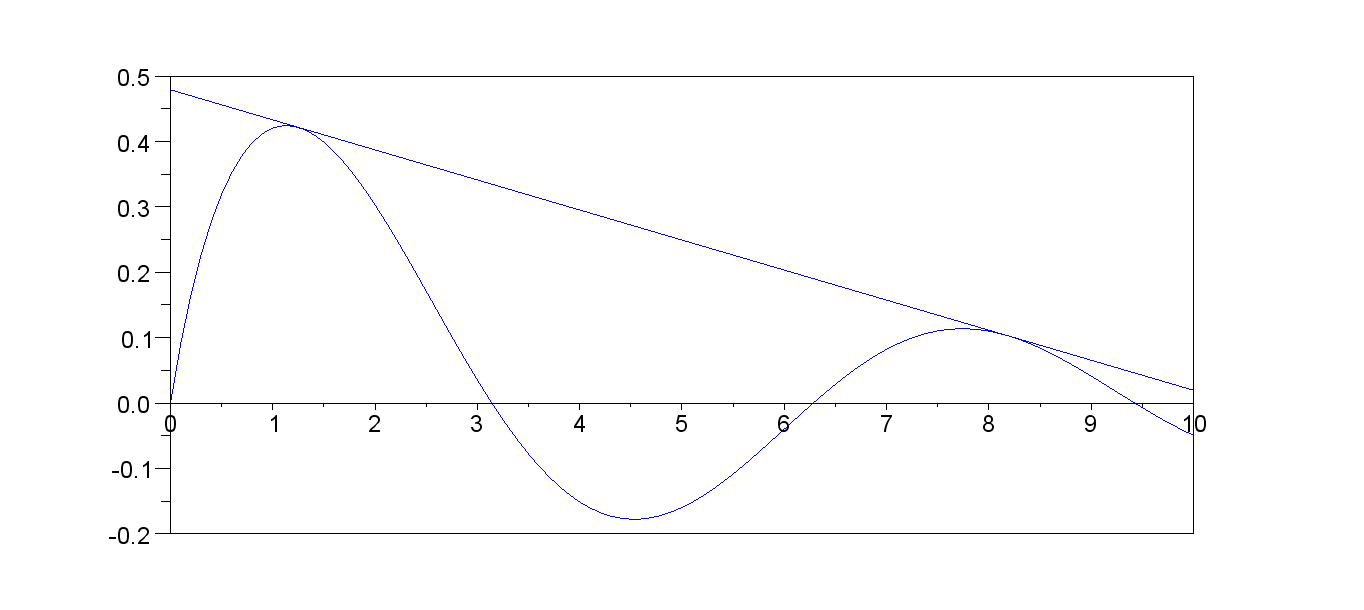
\includegraphics[width=\textwidth]{cap_nlinsis/pics/curva_Q23}
		\caption{Reta bitangente a uma curva.}
		\label{pic:bitang}
	\end{figure}

 \begin{resp}
  $y=mx+b$ com $m\approx - 0.0459710 $ e $b\approx 0.479237$
 
 Uma metodologia possível para resolver este problema é dada a seguir:

Sejam $x_1$ e $x_2$ as abscissas dos dois pontos em que a reta tangencia a curva. A equação da reta bitangente assume a seguinte forma:
$$y=f(x_1) + m(x-x_1) $$
onde o coeficiente angular $m$ é dado por
$$m=\frac{f(x_2)-f(x_1)}{x_2-x_1}$$

Da condição de tangência, temos que o coeficiente angular da reta, $m$, deve igual à derivada da função $f(x)$ nos dois pontos de tangência.
$$m=f'(x_1)=f'(x_2)$$
E sabemos que:
$$f'(x)=\frac{\cos(x)}{1+x}-\frac{\sin(x)}{(1+x)^2}.$$

Assim, podemos reescrever o problema como
\begin{eqnarray*}
\frac{\cos(x_1)}{1+x_1}-\frac{\sin(x_1)}{(1+x_1)^2}-\frac{\cos(x_2)}{1+x_2}+\frac{\sin(x_2)}{(1+x_2)^2}=0\\
\frac{\cos(x_1)}{1+x_1}-\frac{\sin(x_1)}{(1+x_1)^2}-\frac{f(x_2)-f(x_1)}{x_2-x_1}=0
\end{eqnarray*}
Este é um sistema não-linear de duas incógnitas.

Os valores iniciais para o método podem ser obtidos do gráfico buscando valores próximos aos dois primeiros pontos de máximos. Por exemplo: $x_1^{(0)}=1$ e $x_2^{(0)}=8$. Obtemos $x_1\approx 1,2464783$ e $x_2\approx 8,1782997$ e $m$ pode ser obtido através desses valores.


\end{resp}

\begin{figure}
        \centering
	    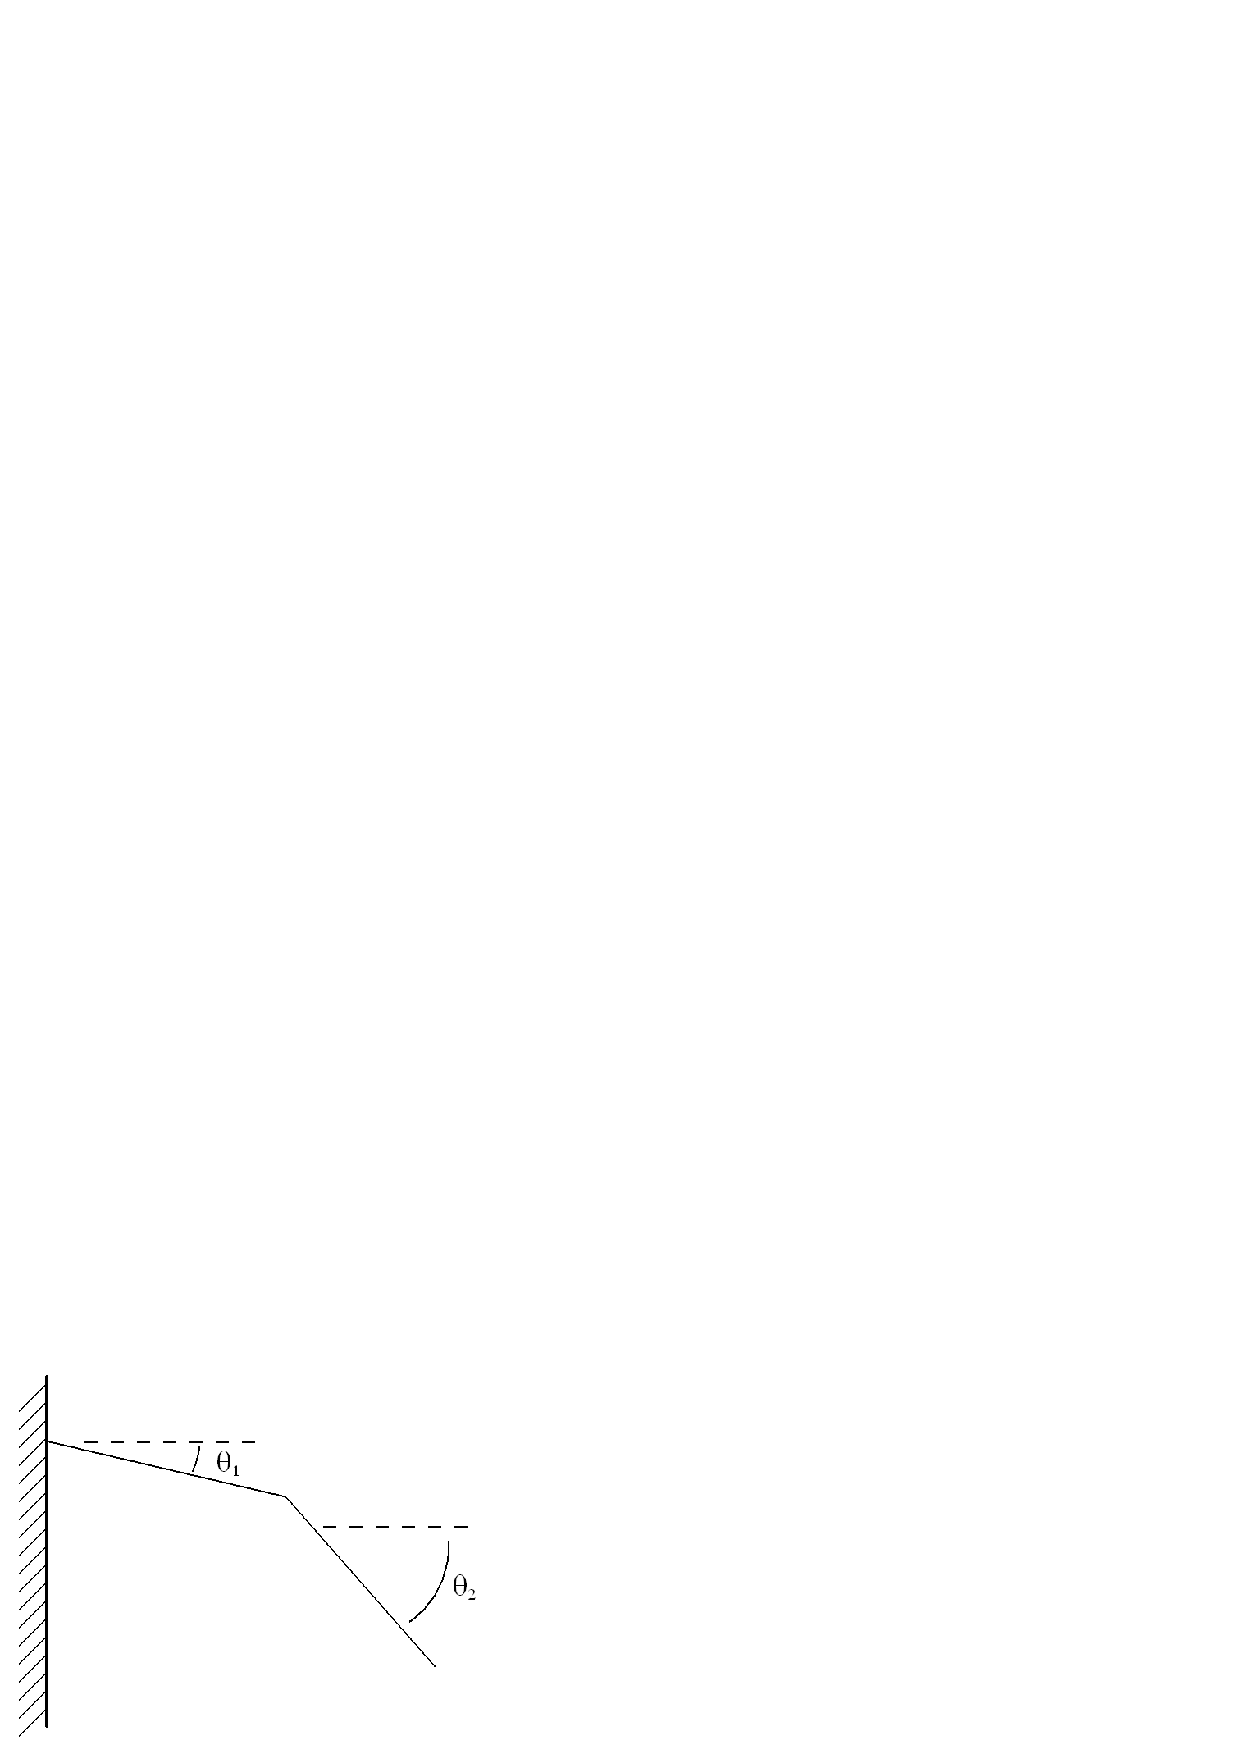
\includegraphics[width=.5\textwidth]{cap_nlinsis/pics/dois_segmentos}
		\caption{Sistema mecânico com dois segmentos.}
		\label{pic:dois_segmentos}
	\end{figure}

\begin{exer}{(Estática)}\label{prob:dois_segmentos} Considere o sistema mecânico constituído de dois segmentos de mesmo comprimento $L$ presos entre si e a uma parede por articulações conforme a figura \ref{pic:dois_segmentos}.

O momento em cada articulação é proporcional à deflexão com constante de proporcionalidade $k$. Os segmentos são feitos de material homogêneo de peso $P$. A condição de equilíbrio pode ser expressa em termos dos ângulos $\theta_1$ e $\theta_2$ conforme:
\begin{eqnarray*}
k\theta_1&=& \frac{3PL}{2}\cos\theta_1 + k\left(\theta_2-\theta_1\right)\\
k\left(\theta_2-\theta_1\right)&=& \frac{PL}{2}\cos\theta_2
\end{eqnarray*}
Considere $P=100N$, $L=1m$ e calcule os ângulos $\theta_1$ e $\theta_2$ quando:
\begin{itemize}
\item[a)] $k=1000$ Nm/rad
\item[b)] $k=500$ Nm/rad
\item[c)] $k=100$ Nm/rad
\item[d)] $k=10$ Nm/rad
\end{itemize}
\noindent {\bf Obs:}Você deve escolher valores para iniciar o método. Como você interpretaria fisicamente a solução para produzir palpites iniciais satisfatórios? O que se altera entre o caso a e o caso d?
\end{exer}

\begin{resp}
$\left(0.1956550;0.2441719 \right)$, $\left(0.3694093;0.4590564\right) $, $\left( 0.9990712;1.1865168  \right)$ e $\left(1.4773606;1.5552232 \right)$
\end{resp}


\begin{exer}{(estática - problemas de três variáveis)} Considere, agora, o sistema mecânico semelhante ao do problema \ref{prob:dois_segmentos}, porém constituído de três segmentos de mesmo comprimento $L$ presos entre si e a uma parede por articulações.

O momento em cada articulação é proporcional à deflexão com constante de proporcionalidade $k$. Os segmentos são feitos de material homogêneo de peso $P$. A condição de equilíbrio pode ser expressa em termos dos ângulos $\theta_1$, $\theta_2$ e $\theta_3$ conforme:
\begin{eqnarray*}
k\theta_1&=& \frac{5PL}{2}\cos\theta_1 + k\left(\theta_2-\theta_1\right)\\
k\left(\theta_2-\theta_1\right)&=& \frac{3PL}{2}\cos\theta_2+k\left(\theta_3-\theta_2\right)\\
k\left(\theta_3-\theta_2\right)&=& \frac{PL}{2}\cos\theta_3
\end{eqnarray*}
Considere $P=10$N, $L=1$m e calcule os ângulos $\theta_1$, $\theta_2$ e $\theta_3$ quando:
\begin{itemize}
\item[a)] $k=1000$Nm/rad
\item[b)] $k=100$Nm/rad
\item[c)] $k=10$Nm/rad
\end{itemize}
\end{exer}
\begin{resp}
$\left(0.0449310; 0.0648872; 0.0698750  \right)$, $\left(0.3981385; 0.5658310; 0.6069019  \right)$, \\
$\left(1.1862966;1.4348545;1.480127  \right)$
\end{resp}


\begin{figure}
        \centering
	    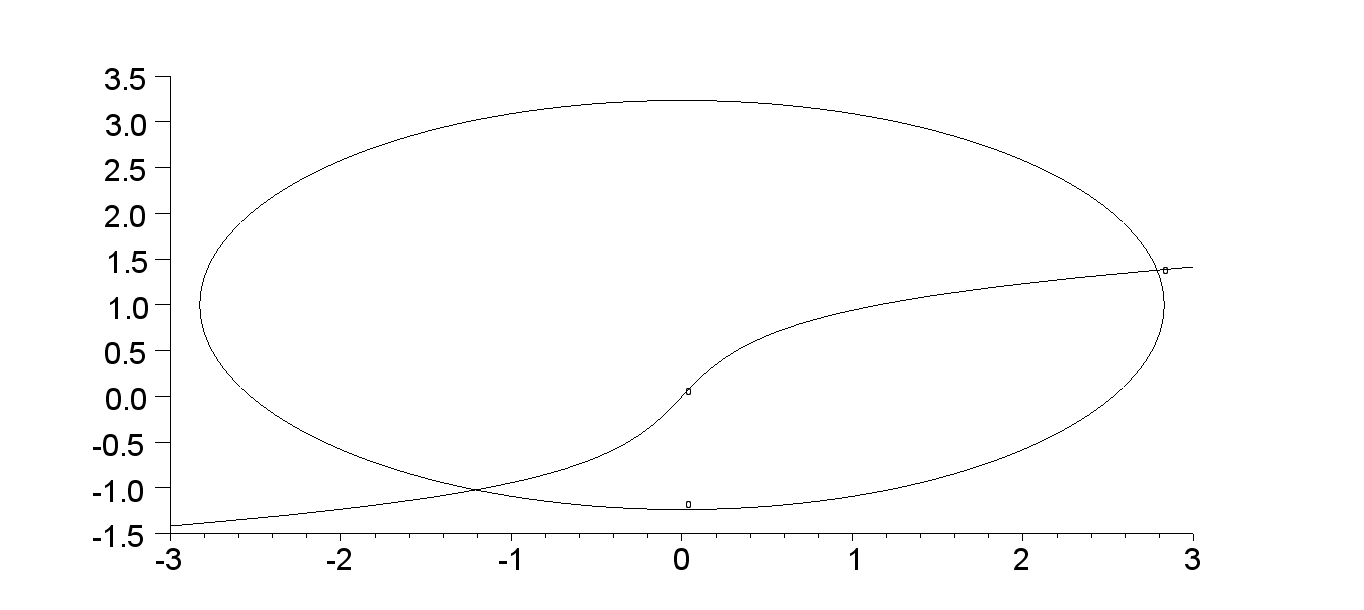
\includegraphics[width=.5\textwidth]{cap_nlinsis/pics/inter_curvas}
		\caption{intersecção entre duas curvas.}
		\label{pic:inter_curvas}
	\end{figure}

\begin{exer}  Considere o problema de encontrar os pontos de intersecção das curvas descritas por (ver figura \ref{pic:inter_curvas}):
\begin{eqnarray*}
\frac{x^2}{8}+\frac{(y-1)^2}{5}&=&1\\~\\
\tan^{-1}(x)+x&=&y+y^3
\end{eqnarray*}
 Com base no gráfico, encontre soluções aproximadas para o problema e use-as para iniciar o método de Newton-Raphson. Encontre as raízes com erro inferior a $10^{-5}$.
\end{exer}

\begin{resp}
$\left(-1,2085435, -1,0216674 \right)$ e $\left(2,7871115, 1,3807962\right)$
\ifisscilab
Exemplo de implementação:
\begin{verbatim}
function z=f(x,y)
    z=x^2/8+(y-1)^2/5-1
endfunction
function z=g(x,y)
    z=atan(x)+x-y-y^3
endfunction

contour([-3:.1:3],[-2:.1:4],f,[0 0])
contour([-3:.1:3],[-2:.1:4],g,[0 0])

function y=F(x)
    y(1)=f(x(1),x(2))
    y(2)=g(x(1),x(2))
endfunction
function y=JF(x)
    y(1,1)=x(1)/4
    y(1,2)=2*(x(2)-1)/5
    y(2,1)=1/(1+x(1)^2)+1
    y(2,2)=-1-3*x(2)^2
endfunction

//primeiro ponto
//x=[-1.2;-1.0]

//segundo ponto
//x=[2.8;1.4]

x=x-JF(x)\F(x)   // 4 vezes
\end{verbatim}
\fi
\end{resp}




\begin{exer} Considere o sistema de equações dado por
\begin{eqnarray*}
\frac{(x-3)^2}{16}+\frac{(y-1)^2}{36}&=&1\\
\tanh(x)+x&=&2\sin y-0.01y^3
\end{eqnarray*}
Usando procedimentos analíticos, determine uma região limitada do plano onde se encontram necessariamente todas as raízes do problema.
Encontre as raízes desse sistema com pelo menos quatro dígitos significativos corretos usando o método de Newton. Você deve contruir o método de Newton indicando as funções envolvidas e calculando a matriz jacobiana analiticamente. Use que $\frac{d}{du}\tanh u = 1-\tanh^2u$, se precisar.
\end{exer}
\begin{resp}
 A primeira curva trata-se de uma elipse de centro $(3,1)$ e semi-eixos 4 e 6, portanto seus pontos estão contidos no retângulo $-1\leq x \leq 7$ e $-5\leq y \leq 7$. 

A soluções são $\left( -0,5384844 , -1,7978634\right)$ e $\left(2,8441544, 6,9954443\right)$.

\ifisscilab
Uma possível implementação é
\begin{verbatim}
    
function z=f(x,y)
    z=(x-3)^2/16+(y-1)^2/36-1
endfunction

function z=g(x,y)
    z=atan(x)+x-sin(y)-0.01*y^3
endfunction

contour([-1:.1:7],[-5:.1:7],f,[0 0])
contour([-1:.1:7],[-5:.1:7],g,[0 0])
    
function y=F(x)
    y(1)=f(x(1),x(2))
    y(2)=g(x(1),x(2))
endfunction
function y=JF(x)
    y(1,1)=(x(1)-3)/8
    y(1,2)=(x(2)-1)/18
    y(2,1)=1/(1+x(1)^2)+1
    y(2,2)=-cos(x(2))-0.03*x(2)^2
endfunction    
 \end{resp}
    
//primeiro ponto
//x=[-.5;-2.0]

//segundo ponto
//x=[3;7]

x=x-JF(x)\F(x)   // 4 vezes
 \end{verbatim}
 \fi
 \end{resp}



\begin{exer}(Otimização)\label{nlinsis:usinas} Uma indústria consome energia elétrica de três usinas fornecedoras. O custo de fornecimento em reais por hora como função da potência consumida em kW é dada pelas seguintes funções
\begin{eqnarray*}
C_1(x)&=&10+.3x+10^{-4}x^2+3.4\cdot 10^{-9}x^4\\
C_2(x)&=&50+.25x+2\cdot 10^{-4}x^2+4.3\cdot 10^{-7}x^3\\
C_3(x)&=&500+.19x+5\cdot 10^{-4}x^2+1.1\cdot 10^{-7}x^4
\end{eqnarray*}
Calcule a distribuição de consumo que produz custo mínimo quando a potência total consumida é $1500kW$. Dica: Denote por $x_1$, $x_2$ e $x_3$ as potências consumidas das usinas 1, 2 e 3, respectivamente.  O custo total será dado por $C(x_1,x_2,x_3)=C_1(x_1)+C_2(x_2)+C_3(x_3)$ enquanto o consumo total é $x_1+x_2+x_3=1500$. Isto é, queremos minimizar a função custo total dada por:
$$C(x_1,x_2,x_3)=C_1(x_1)+C_2(x_2)+C_3(x_3)$$
restrita à condição
$$G(x_1,x_2,x_3)=x_1+x_2+x_3-1500=0.$$
Pelos multiplicadores de Lagrange, temos que resolver o sistema dado por:
\begin{eqnarray*}
\nabla C(x_1,x_2,x_3) &=& \lambda \nabla G(x_1,x_2,x_3)\\
G(x_1,x_2,x_3)&=&0
\end{eqnarray*}
\end{exer}

\begin{resp}
 $(x_1,x_2,x_3)\approx (453,62,~ 901,94,~ 144,43)$
\end{resp}


\begin{exer} \label{nlinsis:prob_ajuste_eax} Encontre a função do tipo $f(x)=Ab^{x}$ que melhor aproxima os pontos $(0,~3,1)$, $(1,~4,4)$ e $(2,~6,7)$ pelo critério dos mínimos quadrados. Dica: Você deve encontrar os valores de $A$ e $b$ que minimizam o resíduo dado por
$$R=\left[3,1-f(0)\right]^2+\left[4,4-f(1)\right]^2+\left[6,7-f(2)\right]^2.$$
{\bf Dica:} Para construir aproximações para resposta e iniciar o método, considere a função $f(x)=Ab^x$ que passa pelo primeiro e terceiro ponto.
\end{exer}
\begin{resp}
Incialização do método: $A^{(0)}= 3,1$ e $b^{(0)}= \sqrt{\frac{6,7}{3,1}}$
$A\approx  3.0297384 $ e $b\approx 1.4835346$.
\end{resp}


 
 
 \begin{exer}Encontre o valor máximo da função $$f(x,y)=-x^4-y^6+3xy^3-x$$ na região $(x,y)\in [-2,0]\times [-2,0]$
 seguindo os seguintes passos:
\begin{itemize}
  \item[a)] Defina a função $z=f(x,y)=-x^4-y^6+3xy^3-x$ e trace o gráfico de contorno na região. 
  \item[b)] Com base no gráfico, encontre valores aproximados para as coordenadas $xy$ do ponto de máximo.
  \item[c)] Sabendo que o ponto de máximo acontece quando o gradiente é nulo, escreva o problema como um sistema de duas equações não lineares e duas incógnitas.
  \item[d)] Implemente o método de Newton.
\end{itemize}
\end{exer}
 \begin{resp}
 $f(-1,1579702, -1,2020694)\approx 2.376985$

\ifisscilab
Um exemplo de implementação no Scilab é:
\begin{verbatim}
deff('z=f(x,y)','z=-x^4-y^6+3*x*y^3-x')
contour([-2:.01:0],[-2:.01:0],f,[ 0:.2: 3])
deff('z=F(x)','z=[-4*x(1)^3+3*x(2)^3-1;-6*x(2)^5+9*x(1)*x(2)^2]')
deff('z=JF(x)','z=[-12*x(1)^2,9*x(2)^2;9*x(2)^2,-30*x(2)^4+18*x(1)*x(2)]')
x=[-1.2;-1.2]
x=x-JF(x)\F(x)
x=x-JF(x)\F(x)
x=x-JF(x)\F(x)
x=x-JF(x)\F(x)
mprintf('f(%f,%f)=%f',x(1),x(2),f(x(1),x(2)))
\end{verbatim}
\fi
\end{resp} 

 
 
 \begin{exer}A função $f(x,y,z)=\sin(x)+\sin(2y)+\sin(3z)$ possui um máximo quando $x=\pi/2$, $y=\pi/4$ e $z=\pi/6$. Calcule numericamente este ponto.
 \end{exer}

 
 \begin{exer}\label{prob_sis3} Encontre as raizes do problema
 \begin{eqnarray*}
 3x-\cos(yz+z)-1/2&=&0\\
 4x^2-25y^2+0.4y+2&=&0\\
 e^{-xy}+2x-5z&=&10
 \end{eqnarray*}
 no cubo $|x|<2, |y|<2, |z|<2.$
 Dica: Reduza a um problema de duas incógnitas e use recursos gráficos para aproximar as raízes na região.
 \end{exer}
 
 \begin{resp}
 $x\approx 0,2982646, y\approx -0,2990796, z\approx- 1,6620333$  e $x\approx -0,0691328, y\approx 0,2923039, z\approx -0,8235705$.
 \end{resp}


\begin{exer}  Considere o seguinte sistema de equações não-lineares:
\begin{eqnarray}
x_1-x_2&=&0\nonumber\\
-x_{j-1}+5(x_j+x_j^3)-x_{j+1}&=&10\exp(-j/3),~~ 2\leq j \leq 10\nonumber\\
x_{11}&=&1
\end{eqnarray}
\begin{itemize}
\item [a)] Escreva este sistema na forma $F(x)=0$ onde $x=\left[\begin{array}{c} x_1\\ x_2\\ \vdots \\ x_{11}\end{array}\right]$ e calcule analiticamente a matriz jacobiana $\frac{\partial (F_1,\ldots, F_{11})}{\partial (x_1,\ldots x_{11})}$. Dica: Use a regularidade nas expressões para abreviar a notação.
\item [b)] Construa a iteração para encontrar a única solução deste problema pelo método de Newton e, usando esse método, encontre uma solução aproximada com erro absoluto inferior a $10^{-4}$.
\end{itemize}
\end{exer}

\begin{resp}
$$F\left(x\right)=\left[
\begin{array}{c}
x_1-x_2\\[.2cm]
-x_{1}+5(x_2+x_2^3)-x_{3}-10\exp(-2/3)\\[.2cm]
-x_{2}+5(x_3+x_3^3)-x_{4}-10\exp(-3/3)\\[.2cm]
-x_{3}+5(x_4+x_4^3)-x_{5}-10\exp(-4/3)\\[.2cm]
\vdots\\
-x_{9}+5(x_{10}+x_{10}^3)-x_{11}-10\exp(-10/3)\\[.2cm]
x_{11}-1
\end{array}\right] $$

$$J_F(x)=\left[
\begin{array}{ccccccc}
1& -1 &0 &0 &0&\ldots & 0\\[.2cm]
-1&5(1+3x_2^2)& -1&0&0&\ldots & 0\\[.2cm]
0&-1&5(1+3x_3^2)& -1&0&\ldots & 0\\[.2cm]
0&0&-1&5(1+3x_4^2)& -1&\ldots & 0\\[.2cm]
\vdots &\vdots &\vdots &\vdots &&\ddots&\vdots\\[.2cm]
0&0&0&0&0&\cdots&1
\end{array}
\right]
$$

\ifisscilab
Exemplo de implementação no Scilab:
\begin{verbatim}
function y=F(x)
    y(1)=x(1)-x(2)
    for j=2:10
        y(j)=-x(j-1)+5*(x(j)+x(j)^3)-x(j+1)-10*exp(-j/3)
    end
    y(11)=x(11)-1
endfunction

function y=JF(x)
    y=zeros(11,11)

    y(1,1)=1
    y(1,2)=-1
    for j=2:10

        y(j,j-1)=-1
        y(j,j)=5*(1+3*x(j)^2)
        y(j,j+1)=-1
    end
    y(11,11)=1
endfunction
\end{verbatim}
\fi

Resposta final: 0,80447, 0,80447, 0,68686, 0,57124, 0,46535,
0,37061, 0,28883, 0,22433, 0,19443, 0,28667,  1
\end{resp}


\begin{exer} Considere a função
$$f(x,y)=\frac{e^{-(x-1)^2-(y-2)^2}}{1+x^2+y^2}$$
\begin{itemize}
\item[a)] Encontre o valor máximo desta função.
\item[b)] Usando multiplicadores de Lagrange, encontre o valor máximo desta função restrito à condição $$(x-1)^2+(y-2)^2=1.$$
\item[c)] Parametrize a circunferência para transformar o problema de máximo com restrição em um problema de uma única variável. Resolva usando as técnicas de equações lineares de uma variável.
\end{itemize}

\end{exer}
\begin{resp}
$f(0,8108792, 1,6217584)\approx 0,1950369$ e $f(0,5527864, 1,1055728 )\approx 0,1455298 $
\end{resp}



\section{Linearização de uma função de várias variáveis}
Nesta seção, discutimos de forma distinta e mais rigorosa os conceitos de matriz jacobiana e linearização de uma função de várias variáveis.\index{matriz!jacobiana}
\subsection{Gradiente}

Considere primeiramente uma função $f:\mathbb{R}^n\to \mathbb{R}$, ou seja, uma função que mapeia n variáveis reais em um único real, por exemplo:
$$f(x)=x_1^2+x_2^2/4$$

Para construirmos a linearização, fixemos uma direção no espaço $\mathbb{R}^n$, ou seja, um vetor $v$:
$$v=[v_1,  v_2,  \cdots,  v_n]^T$$

Queremos estudar como a função $f(x)$ varia quando ``andamos'' na direção $v$ a partir do ponto $x^{(0)}$. Para tal, inserimos um parâmetro  real pequeno $h$, dizemos que $$x=x^{(0)}+hv$$ e definimos a função auxiliar
$$g(h)=f(x^{0}+hv).$$
Observamos que a função $g(h)$ é uma função de $\mathbb{R}$ em $\mathbb{R}$.

A linearização de $g(h)$ em torno de $h=0$ é dada por

$$g(h)=g(0) + hg'(0) +O(h^2)$$
Observamos que $g(h)=f(x^{(0)}+hv)$ e $g(0)=f(x^{(0)})$. Precisamos calcular $g'(0)$:

\begin{eqnarray*}
g'(h)=\frac{d}{dh}g(h)=\frac{d}{dh}f(x^{(0)}+hv).
\end{eqnarray*}
Pela regra da cadeia temos:
\begin{eqnarray*}
\frac{d}{dh}f(x^{(0)}+hv)= \sum_{j=1}^n \frac{\partial f}{\partial x_j}\frac{d x_j}{d h}.
\end{eqnarray*}

Observamos que $x_j=x^{(0)}_j+hv_j$, portanto
$$\frac{d x_j}{d h}=v_j$$
Assim:
\begin{eqnarray*}
\frac{d}{dh}f(x^{(0)}+hv)= \sum_{j=1}^n \frac{\partial f}{\partial x_j}v_j.
\end{eqnarray*}
Observamos que esta expressão pode ser vista como o produto interno entre o gradiente de $f$ e o vetor $v$:
\begin{eqnarray*}
\nabla f = \left[
\begin{matrix}
\frac{\partial f}{\partial x_1} \\
\frac{\partial f}{\partial x_2} \\
\vdots\\
\frac{\partial f}{\partial x_n}
\end{matrix}
\right] \qquad v=\left[
\begin{matrix}
v_1\\
v_2\\
\vdots\\
v_n
\end{matrix}
\right]
\end{eqnarray*}

Na notação cálculo vetorial escrevemos este produto interno como $\nabla f \cdot v = v \cdot \nabla f$ na notação de produto matricial, escrevemos $\left(\nabla f\right)^T v = v^T\nabla f$. Esta quantidade é conhecida como {\bf derivada direcional} de $f$ no ponto $x^{(0)}$ na direção $v$, sobretudo quando $\|v\|=1$.


Podemos escrever a linearização
$g(h)=g(0) + hg'(0) +O(h^2)$ como
$$f(x^{(0)}+hv)=f(x^{(0)})+ h \nabla^T\! f(x^{(0)})\!~v  + O(h^2)$$

Finalmente, escrevemos $x=x^{(0)}+hv$, ou seja, $hv=x-x^{(0)}$
$$f(x)=f(x^{(0)})+ \nabla^T\! f(x^{(0)})\!~(x-x^{(0)})   + O(\|x-x^{(0)}\|^2)$$

\begin{obs} Observe a semelhança com a linearização no caso em uma dimensão. A notação $\nabla^T\! f(x^{(0)})$ é o transposto do vetor gradiente associado à função $f(x)$ no ponto $x^{(0)}$:
$$\nabla^T f(x^{(0)})=\left[\frac{\partial f\left(x^{(0)}\right)}{\partial x_1},~~ \frac{\partial f\left(x^{(0)}\right)}{\partial x_2},~~ \cdots,~\frac{\partial f\left(x^{(0)}\right)}{\partial x_n}\right]$$
\end{obs}

\subsection{Matriz jacobiana}\index{matriz!jacobiana}
Interessamo-nos, agora, pela linearização da função $F:\mathbb{R}^n\to \mathbb{R}^n$. Lembramos que $F(x)$ pode ser escrita como um vetor de funções $f_j:\mathbb{R^n}\to\mathbb{R}$:
\begin{equation*}
  F(x)=\left[\begin{matrix}
      f_1(x)\\
      f_2(x)\\
      \vdots\\
      f_n(x)
    \end{matrix}\right]
\end{equation*}
Linearizando cada uma das funções $f_j$, temos:
\begin{eqnarray*}
F(x)&=&\underbrace{\left[
\begin{array}{c}
f_1\left(x^{(0)}\right)+\nabla^T\! f_1(x^{(0)})\!~\left(x-x^{(0)}\right)   + O(\|x-x^{(0)}\|^2)\\~\\
f_2\left(x^{(0)}\right)+\nabla^T\! f_2(x^{(0)})\!~\left(x-x^{(0)}\right)   + O(\|x-x^{(0)}\|^2)\\~\\
\vdots\\~\\
f_n\left(x^{(0)}\right)+\nabla^T\! f_n(x^{(0)})\!~\left(x-x^{(0)}\right)   + O(\|x-x^{(0)}\|^2)
\end{array}
\right]}_{\text{Vetor coluna}}
\end{eqnarray*}
ou, equivalentemente:
\begin{eqnarray*}
 F(x) &=&\underbrace{\left[
\begin{array}{c}
f_1\left(x^{(0)}\right)\\~\\
f_2\left(x^{(0)}\right)\\~\\
\vdots\\~\\
f_n\left(x^{(0)}\right)
\end{array}
\right]}_{\text{Vetor coluna}}+
\underbrace{\left[
\begin{array}{c}\nabla^T\! f_1(x^{(0)})\\~~\\
\nabla^T\! f_2(x^{(0)})\\~~\\
\vdots\\~~\\
\nabla^T\! f_n(x^{(0)})
\end{array}
\right]}_{\text{Matriz jacobiana}}\underbrace{\left(x-x^{(0)}\right)}_{\text{Vetor coluna}}+O(\|x-x^{(0)}\|^2)
\end{eqnarray*}

Podemos escrever a linearização de $F(x)$ na seguinte forma mais enxuta:
$$F(x)=F\left(x^{(0)}\right)+ J_F(x^{(0)})\left(x-x^{(0)}\right) + O\left(\left\|x-x^{(0)}\right\|^2\right) $$

A matriz jacobiana $J_F$ é matriz cujas linhas são os gradientes transpostos de $f_j$, ou seja:
$$J_F= \frac{\partial(f_1,f_2,\ldots,f_n)}{\partial(x_1,x_2,\ldots,x_n)}=\left[
\begin{array}{ccccc}
\frac{\partial f_1}{\partial x_1}&\frac{\partial f_1}{\partial x_2}&\cdots&\frac{\partial f_1}{\partial x_n}\\~\\
\frac{\partial f_2}{\partial x_1}&\frac{\partial f_2}{\partial x_2}&\cdots&\frac{\partial f_2}{\partial x_n}\\~\\
\vdots&\vdots&\ddots&\vdots\\~\\
\frac{\partial f_n}{\partial x_1}&\frac{\partial f_n}{\partial x_2}&\cdots&\frac{\partial f_n}{\partial x_n}\\~\\
\end{array}
\right]
$$
A matriz jacobiana de uma função ou simplesmente, o jacobiano de uma função $F(x)$ é a matriz formada pelas suas derivadas parciais:
$$\left(J_F\right)_{ij}=\frac{\partial f_i}{\partial x_j}$$


\begin{ex} Calcule a matriz jacobiana da função
$$F(x)=\left[
\begin{array}{c}
\frac{x_1^2}{3}+x_2^2-1\\~\\
x_1^2+\frac{x_2^2}{4}-1
\end{array}
\right]$$

$$J_F=\left[
\begin{array}{cc}
\frac{\partial f_1}{\partial x_1} & \frac{\partial f_1}{\partial x_2}\\~\\
\frac{\partial f_2}{\partial x_1} & \frac{\partial f_2}{\partial x_2}\\
\end{array}
\right]=\left[
\begin{array}{cc}
\frac{2x_1}{3} & 2x_2\\~\\
2x_1&\frac{x_2}{2}
\end{array}
\right]
$$
\end{ex}

%\end{document} 

%Este trabalho está licenciado sob a Licença Creative Commons Atribuição-CompartilhaIgual 3.0 Não Adaptada. Para ver uma cópia desta licença, visite http://creativecommons.org/licenses/by-sa/3.0/ ou envie uma carta para Creative Commons, PO Box 1866, Mountain View, CA 94042, USA.

\documentclass[main.tex]{subfiles}

\begin{document}

\chapter{Aproximação de funções}\index{aproximação!de funções}

O problema geral da interpolação pode ser definido da seguinte forma:

Seja $\mathcal{F}$ uma família de funções $f:D\to E$ e $\left\{(x_i,y_i)\right\}_{i=1}^N$ um conjunto de pares ordenados tais que $x_i\in D$ e $y_i\in E$, encontrar uma função $f$ da família dada tal que $f(x_i)=y_i$ para cada $1\leq i \leq N$.
\begin{ex} Encontrar uma função $f(x)$ da forma $f(x)=a e^{bx}$ onde $a$ e $b$ são constantes tal que $f(1)=1$ e $f(2)=5$. Este problema equivale a resolver o seguinte sistema de equações:
\begin{eqnarray*}
ae^b&=&1\\
ae^{2b}&=&5
\end{eqnarray*}
Dividindo a segunda equação pela primeira, temos $e^b=5$, logo, $b=\ln(5)$. Substituindo este valor em qualquer das equações, temos $a=\frac{1}{5}$. Assim $$f(x)=\frac{1}{5}e^{\ln(5) x}=\frac{1}{5}5^x=5^{x-1}.$$
\end{ex}

\begin{ex} Encontrar a função polinomial do tipo $f(x)=a+bx+cx^2$ que passe pelos pontos $(-1,2)$, $(0,1)$, $(1,6)$. Observamos que podemos encontrar os coeficientes $a$, $b$ e $c$ através do seguinte sistema linear:
\begin{eqnarray*}
a-b+c&=&2\\
a&=&1\\
a+b+c&=&6
\end{eqnarray*}
cuja solução é dada por $a=1$, $b=2$ e $c=3$. Portanto $$f(x)=1+2x+3x^2.$$
\end{ex}

\section{Interpolação polinomial}\index{interpolação!polinomial}

Interpolação polinomial é o caso particular do problema geral de interpolação quando a família de funções é constituída de polinômios.
\begin{teo}\label{teo_interp_poli} Seja $\{(x_i,y_i)\}_{i=0}^{n}$ um conjunto de $n+1$ pares ordenados de números reais tais que $$i\neq j \Longrightarrow x_i\neq x_j~~~~\hbox{ (i.e. as abscissas são distintas)}$$
então existe um único polinômio $P(x)$ de grau igual ou inferior a $n$ que passa por todos os pontos dados.
\end{teo}
\begin{proof} Observamos que o problema de encontrar os coeficientes $a_0$, $a_1$,\ldots, $a_n$ do polinômio
$$P(x)=a_0+a_1x+a_2x^2+\cdots a_n x^n=\sum_{k=0}^n a_k x^k$$
tal que $P(x_i)=y_i$ é equivalente ao seguinte sistema linear de $n+1$ equações e $n+1$ incógnitas:
\begin{eqnarray*}
a_0+a_1x_0+a_2x_0^2+\cdots +a_n x_0^n&=&y_0\\
a_0+a_1x_2+a_2x_1^2+\cdots +a_n x_1^n&=&y_1\\
&\vdots&\\
a_0+a_1x_n+a_2x_n^2+\cdots +a_n x_n^n&=&y_n
\end{eqnarray*}
que pode ser escrito na forma matricial como
$$\left[
\begin{array}{ccccc}
1 & x_0 & x_0^2 & \cdots & x_0^n\\
1 & x_1 & x_1^2 & \cdots & x_1^n\\
1 & x_2 & x_2^2 & \cdots & x_2^n\\
\vdots&\vdots&\vdots&\ddots&\vdots\\
1 & x_n & x_n^2 & \cdots & x_n^n
\end{array}
\right]
\left[
\begin{array}{c}
a_0\\a_1\\a_2\\ \vdots \\a_n
\end{array}
\right]=
\left[
\begin{array}{c}
y_0\\y_1\\y_2\\ \vdots \\y_n
\end{array}
\right]
$$
A matriz envolvida é uma matriz de Vandermonde de ordem $n+1$ cujo determinante é dado por
$$\prod_{0\leq i<j\leq n}\left(x_j-x_i\right)$$
É fácil ver que se as abscissas são diferentes dois a dois, então o determinante é não-nulo. Disto decorre que o sistema possui um a solução e que esta solução é única.
\end{proof}

\begin{ex} Encontre o polinômio da forma $P(x)=a_0+a_1x+a_2x^2+a_3x^3$ que passa pelos pontos
$$(0,1),(1,2),(2,4),(3,8)$$
Este problema é equivalente ao seguinte sistema linear:
\begin{eqnarray*}
a_0&=&1\\
a_0+a_1+a_2+a_3&=&2\\
a_0+2a_1+4a_2+8a_3&=&4\\
a_0+3a_1+9a_2+27a_3&=&8
\end{eqnarray*}
cuja solução é $a_0=1$, $a_1=\frac{5}{6}$, $a_2=0$ e $a_3=\frac{1}{6}$. Portanto
$$P(x)=1+\frac{5}{6}x+\frac{1}{6}x^3$$
\end{ex}

\begin{ex} Encontre o polinômio da forma $P(x)=a_0+a_1x+a_2x^2+a_3x^3$ que passa pelos pontos
$$(0,0),(1,1),(2,4),(3,9)$$
Este problema é equivalente ao seguinte sistema linear:
\begin{eqnarray*}
a_0&=&0\\
a_0+a_1+a_2+a_3&=&1\\
a_0+2a_1+4a_2+8a_3&=&4\\
a_0+3a_1+9a_2+27a_3&=&9
\end{eqnarray*}
cuja solução é $a_0=0$, $a_1=0$, $a_2=1$ e $a_3=0$. Portanto
$$P(x)=x^2$$
\end{ex}

Esta abordagem direta que fizemos ao calcular os coeficientes do polinômio na base canônica se mostra ineficiente quando o número de pontos é grande e quando existe grande discrepância nas abscissas. Neste caso a matriz de Vandermonde é mal-condicionada (ver \cite{Gautschi}), acarretando um aumento dos erros de arredondamento na solução do sistema.

Uma maneira de resolver este problema é escrever o polinômio em uma base que produza um sistema mais bem-condicionado.

\section{Diferenças divididas de Newton}\index{diferenças divididas de Newton}
O método das diferenças divididas de Newton consistem em construir o polinômio interpolador da seguinte forma:
\begin{align*}
P(x) &= a_0 + a_1 (x-x_0) + a_2 (x-x_0)(x-x_1) + \cdots \\
&+ a_n (x-x_0)(x-x_1)\cdots (x-x_{n-1}).
\end{align*}
Assim, o problema de calcular os coeficientes $a_0$, $a_1$, \ldots, $a_n$ é equivalente ao seguinte sistema linear:
\begin{small}
\begin{align*}
a_0 &= y_0\\
a_0+a_1(x_1-x_0) &= y_1\\
a_0+a_1(x_2-x_0)+a_2(x_2-x_0)(x_2-x_1) &= y_2\\
&\vdots\\
a_0+a_1(x_n-x_0)+a_2(x_n-x_0)(x_n-x_1)+\cdots + a_n(x_n-x_0)\cdots (x_n-x_{n-1})
 &= y_n
\end{align*}.  
\end{small}
O qual é equivalente à sua forma matricial:
\begin{small}
  \begin{equation*}
    \begin{bmatrix}
      1 & 0 & 0  & \!\cdots\!&0\\
      1& (x_1-x_0)&0 &\!\cdots\!&0\\
      1&(x_2-x_0)&(x_2-x_0)(x_2-x_1) &\!\cdots\!&0\\
      \vdots&\vdots&\vdots&\!\ddots\!&\vdots\\
      1&(x_n-x_0)&(x_n-x_0)(x_n-x_1) &\!\cdots\!& (x_{n}-x_0)\cdots(x_n-x_{n-1})\\
    \end{bmatrix}\begin{bmatrix}
      a_0\\a_1\\a_2\\ \vdots \\a_n
    \end{bmatrix} = 
    \begin{bmatrix}
      y_0\\y_1\\y_2\\ \vdots \\y_n
    \end{bmatrix}
  \end{equation*}
\end{small}

Este é um sistema triangular inferior que pode ser facilmente resolvido conforme:
\begin{eqnarray*}
a_0&=&y_0\\
a_1&=&\frac{y_1-a_0}{x_1-x_0}=\frac{y_1-y_0}{x_1-x_0}\\
a_2&=&\frac{y_2-a_1(x_2-x_0)-a_0}{(x_2-x_0)(x_2-x_1)}=\frac{\frac{y_2-y_1}{(x_2-x_1)}-\frac{y_1-y_0}{(x_1-x_0)}}{(x_2-x_0)}\\
&\ldots&
\end{eqnarray*}
A solução deste sistema pode ser escrita em termos das Diferenças Divididas de Newton, definidas recursivamente conforme:
\begin{eqnarray*}
f[x_j]&=&y_j\\
f[x_j,x_{j+1}]&=&\frac{f[x_{j+1}]-f[x_j]}{x_{j+1}-x_j}\\
f[x_j,x_{j+1},x_{j+2}]&=&\frac{f[x_{j+1},x_{j+2}]-f[x_j,x_{j+1}]}{x_{j+2}-x_j}\\
&\vdots&
\end{eqnarray*}
Nesta notação, temos
$a_k=f[x_0,x_1,x_2,\ldots,x_k]$

Podemos esquematizar o método na seguinte tabela:
$$
\begin{array}{|c|c|c|c|c|}\hline
 j&x_j&f[x_j]&f[x_{j-1},x_j]&f[x_{j-2},x_{j-1},x_j]\\\hline
&&&&\\
0& x_0 & f[x_0]&&\\
&&&&\\
&&&f[x_0,x_1]=\frac{f[x_1]-f[x_0]}{x_1-x_0}&\\
&&&&\\
1&x_1&f[x_1]&&f[x_0,x_1,x_2]=\frac{f[x_1,x_2]-f[x_0,x_1]}{x_2-x_0}\\
&&&&\\
&&&f[x_1,x_2]=\frac{f[x_2]-f[x_1]}{x_2-x_1}&\\
&&&&\\
2&x_2&f[x_2]&&\\
&&&&\\ \hline
\end{array}
$$

\begin{ex}
Encontrar o polinômio que passe pelos seguintes pontos
$$(-1,3),(0,1),(1,3),(3,43)$$

\begin{equation*}
\begin{array}{|c||c|c|c|c|c|}\hline
 j&x_j&f[x_j]&f[x_{j-1},x_j]&f[x_{j-2},x_{j-1},x_j]&f[x_{j-3},x_{j-2},x_{j-1},x_j]\\\hline
&&&&&\\
0& -1 & 3&&&\\
&&&&&\\
&&&\frac{1-3}{0-(-1)}=-2&&\\
&&&&&\\
1&0&1&&\frac{2-(-2)}{1-(-1)}=2&\\
&&&&&\\
&&&\frac{3-1}{1-0}=2&&\frac{6-2}{3-(-1)}=1\\
&&&&&\\
2&1&3&&\frac{20-2}{3-0}=6&\\
&&&&&\\
&&&\frac{43-3}{3-1}=20&&\\
&&&&&\\
3&3&43&&&\\
&&&&&\\\hline
\end{array}  
\end{equation*}



Portanto
\begin{eqnarray*}
P(x)&=&3-2(x+1)+2(x+1)x+(x+1)x(x-1)\\
&=&x^3+2x^2-x+1
\end{eqnarray*}
\end{ex}

\section*{Exercícios}


\begin{Exercise}\label{exer:interp1}
Considere o seguinte conjunto de pontos: $$(-2,-47),(0,-3),(1,4)(2,41)$$. Encontre o polinômio interpolador usando os métodos vistos. 
\end{Exercise}
\begin{Answer}
  \begin{tiny}
$5x^3+2x-3$    
  \end{tiny}
\end{Answer}

\ifisscilab
\begin{Exercise}
  No \verb+Scilab+, faça um gráfico com os pontos e o polinômio interpolador do Exercício~\ref{exer:interp1}.
\end{Exercise}
\fi

\section{Polinômios de Lagrange}\index{polinômios!de Lagrange}
Outra maneira clássica de resolver o problema da interpolação polinomial é através do polinômios de Lagrange. Dado um conjunto de pontos $\{x_j\}_{j=1}^n$ distintos dois a dois, definimos os polinômios de Lagrange como os polinômios de grau $n-1$ que satisfazem as seguintes condições:
$$
L_k(x_j)=\left\{\begin{array}{rl}
1,&k=j\\
0,&k\neq j
\end{array}
\right.
$$
Assim, a solução do problema de encontrar os polinômios de grau $n-1$ tais $P(x_j)=y_j,j=1,\cdots,n$ é dado por
$$P(x)=y_1L_1(x)+y_2L_2(x)+\cdots +y_nL_n(x)=\sum_{j=1}^n y_j L_j(x)$$

Para construir os polinômios de Lagrange, basta olhar para sua forma fatorada, ou seja:
$$L_k(x)=C_k\prod_{1\leq j \neq k \leq n } (x-x_j)$$
onde o coeficiente $C_k$ é obtido da condição $L_k(x_k)=1$:
$$L_k(x_k)=C_k\prod_{1\leq j \neq k \leq n } (x_k-x_j) \Longrightarrow C_k=\frac{1}{\prod_{1\leq j \neq k \leq n } (x_k-x_j)}$$
Portanto,
$$L_k(x)=\prod_{1\leq j \neq k \leq n } \frac{(x-x_j)}{(x_k-x_j)}$$

\begin{obs} O problema de interpolação quando escrito usando como base os polinômios de Lagrange produz um sistema linear diagonal.
\end{obs}

\begin{ex}Encontre o polinômio da forma $P(x)=a_0+a_1x+a_2x^2+a_3x^3$ que passa pelos pontos
$$(0,0),(1,1),(2,4),(3,9)$$
Escrevemos:
\begin{eqnarray*}
L_1(x)&=& \frac{(x-1)(x-2)(x-3)}{(0-1)(0-2)(0-3)}=-\frac{1}{6}x^3+x^2-\frac{11}{6}x+1\\
L_2(x)&=& \frac{x(x-2)(x-3)}{1(1-2)(1-3)}=\frac{1}{2}x^3-\frac{5}{2}x^2+3x\\
L_3(x)&=& \frac{x(x-1)(x-3)}{2(2-1)(2-3)}=-\frac{1}{2}x^3+2x^2-\frac{3}{2}x\\
L_4(x)&=& \frac{x(x-1)(x-2)}{3(3-1)(3-2)}=\frac{1}{6}x^3-\frac{1}{2}x^2+\frac{1}{3}x
\end{eqnarray*}
Assim temos:
$$P(x)=0\cdot L_1(x)+1\cdot L_2(x)+4\cdot L_3(x)+9\cdot L_4(x)=x^2$$
\end{ex}

\begin{ex}Encontre o polinômio da forma $P(x)=a_0+a_1x+a_2x^2+a_3x^3$ que passa pelos pontos
$$(0,0),(1,1),(2,0),(3,1)$$
Como as abscissas são as mesmas do exemplo anterior, podemos utilizar os mesmos polinômios de Lagrange, assim temos:
$$P(x)=0\cdot L_1(x)+1\cdot L_2(x)+0\cdot L_3(x)+1\cdot L_4(x)=\frac{2}{3}x^3-3x^2+\frac{10}{3}x$$
\end{ex}



\section{Aproximação de funções reais por polinômios interpoladores}\index{aproximação!de funções!por polinômios}

\begin{teo}{\label{teo_interp}}
Dados $n+1$ pontos distintos, $x_0,\ x_1,\ \cdots,\ x_n$, dentro de um intervalo $[a,b]$ e uma função $f$ com $n+1$ derivadas contínuas nesse intervalo ($f\in C^{n+1}[a,b]$), então para cada $x$ em $[a,b]$, existe um número $\xi(x)$ em $(a,b)$ tal que
$$
f(x)=P(x)+\frac{f^{(n+1)}(\xi(x))}{(n+1)!}(x-x_0)(x-x_1)\cdots(x-x_n),
$$
onde $P(x)$ é o polinômio interpolador. Em especial, pode-se dizer que
$$
|f(x)-P(x)|\leq \frac{M}{(n+1)!}\left|(x-x_0)(x-x_1)\cdots(x-x_n)\right|,
$$
onde
$$
M=\max_{x\in[a,b]}|f^{(n+1)}(\xi(x))|
$$
\end{teo}

\begin{ex}
Considere a função $f(x)=\cos(x)$ e o polinômio $P(x)$ de grau 2 tal que $P(0)=\cos(0)=1$, $P(\frac{1}{2})=\cos(\frac{1}{2})$ e $P(1)=\cos(1)$. Use a fórmula de Lagrange para encontrar $P(x)$. Encontre o erro máximo que se assume ao aproximar o valor de $\cos(x)$ pelo de $P(x)$ no intervalo $[0,1]$. Trace os gráficos de $f(x)$ e $P(x)$ no intervalo $[0,1]$ no mesmo plano cartesiano e, depois, trace o gráfico da diferença $\cos(x)-P(x)$. Encontre o erro efetivo máximo $|\cos(x)-P(x)|$.
\end{ex}

\begin{eqnarray*}
P(x)&=&1\frac{(x-\frac{1}{2})(x-1)}{(0-\frac{1}{2})(0-1)}+\cos\left(\frac{1}{2}\right)\frac{(x-0)(x-1)}{(\frac{1}{2}-0)(\frac{1}{2}-1)}+\cos(1)\frac{(x-0)(x-\frac{1}{2})}{(1-0)(1-\frac{1}{2})}\\
&\approx&   1 - 0,0299720583066x - 0,4297256358252x^2
\end{eqnarray*}

\ifisscilab
\begin{verbatim}
L1=poly([.5 1],'x');L1=L1/horner(L1,0)
L2=poly([0 1],'x');L2=L2/horner(L2,0.5)
L3=poly([0 .5],'x');L3=L3/horner(L3,1)
P=L1+cos(.5)*L2+cos(1)*L3
x=[0:.05:1]
plot(x,cos)
plot(x,horner(P,x),'red')
plot(x,horner(P,x)-cos(x))
\end{verbatim}
\fi

Para encontrar o erro máximo, precisamos estimar $|f'''(x)|=|\sin(x)|\leq \sin(1)<0,85$ e
$$
\max_{x\in[0,1]} \left|x\left(x-\frac{1}{2}\right)(x-1)\right|
$$
O polinômio de grau três $Q(x)=x\left(x-\frac{1}{2}\right)(x-1)$ tem um mínimo (negativo) em $x_1=\frac{3+\sqrt{3}}{6}$ e um máximo (positivo) em $x_2=\frac{3-\sqrt{3}}{6}$. Logo:
$$
\max_{x\in[0,1]} \left|x\left(x-\frac{1}{2}\right)(x-1)\right|\leq \max\{|Q(x_1)|,\ |Q(x_2)|\}\approx 0,0481125.
$$
Portanto:
$$
|f(x)-P(x)|< \frac{0,85}{3!}0,0481125\approx 0,0068159<7\cdot 10^{-3}
$$

Para encontrar o erro efetivo máximo, basta encontrar o máximo de $|P(x)-cos(x)|$. O mínimo (negativo) de $P(x)-cos(x)$ acontece em $x_1=4,29\cdot 10^{-3}$ e o máximo (positivo) acontece em $x_2=3,29\cdot 10^{-3}$. Portanto, o erro máximo efetivo é $4,29\cdot 10^{-3}$.

\begin{ex}\label{exemp_simpson}
Considere o problema de aproximar o valor da integral $\int_0^1 f(x)dx$ pelo valor da integral do polinômio $P(x)$ que coincide com $f(x)$ nos pontos $x_0=0$, $x_1=\frac{1}{2}$ e $x_2=1$. Use a fórmula de Lagrange para encontrar $P(x)$. Obtenha o valor de $\int_0^1f(x)dx$ e encontre uma expressão para o erro de truncamento.
\end{ex}
O polinômio interpolador de $f(x)$ é
\begin{eqnarray*}
P(x)&=&f(0)\frac{(x-\frac{1}{2})(x-1)}{(0-\frac{1}{2})(0-1)}+f\left(\frac{1}{2}\right)\frac{(x-0)(x-1)}{(\frac{1}{2}-0)(\frac{1}{2}-1)}+f(1)\frac{(x-0)(x-\frac{1}{2})}{(1-0)(1-\frac{1}{2})}\\
&=&   f(0)(2x^2-3x+1)+f\left(\frac{1}{2}\right)(-4x^2+4x)+f(1)(2x^2-x)
\end{eqnarray*}
e a integral de $P(x)$ é:
\begin{align*}
\int_0^1 P(x)dx &= \left[f(0)\left(\frac{2}{3}x^3 - \frac{3}{2}x^2+x\right)\right]_0^1 + \left[f\left(\frac{1}{2}\right)\left(-\frac{4}{3}x^3+2x^2\right)\right]_0^1 \\
&+ \left[f(1)\left(\frac{2}{3}x^3-\frac{1}{2}x^2\right)\right]_0^1\\
&= f(0)\left(\frac{2}{3}-\frac{3}{2}+1\right)+f\left(\frac{1}{2}\right)\left(-\frac{4}{3}+2\right)+f(1)\left(\frac{2}{3}-\frac{1}{2}\right)\\
&= \frac{1}{6}f(0)+\frac{2}{3}f\left(\frac{1}{2}\right)+\frac{1}{6}f(1)
\end{align*}
Para fazer a estimativa de erro usando o teorema (\ref{teo_interp}), e temos
\begin{eqnarray*}
\left|\int_0^1f(x)dx-\int_0^1 P(x)dx\right|&=&\left|\int_0^1f(x)- P(x)dx\right|\\
&\leq&\int_0^1|f(x)- P(x)|dx\\
&\leq& \frac{M}{6}  \int_0^1\left|x\left(x-\frac{1}{2}\right)(x-1)\right|dx\\
&=& \frac{M}{6}  \left[\int_0^{1/2}x\left(x-\frac{1}{2}\right)(x-1)dx\right.\\
&-&\left.\int_{1/2}^1x\left(x-\frac{1}{2}\right)(x-1)dx\right]\\
&=& \frac{M}{6}  \left[\frac{1}{64}-\left(-\frac{1}{64}\right)\right]=\frac{M}{192}.
\end{eqnarray*}
Lembramos que $M=\max_{x\in[0,1]}|f'''(x)|$.

\begin{obs}Existem estimativas melhores para o erro de truncamento para este esquema de integração numérica. Veremos com mais detalhes tais esquemas na teoria de integração numérica.
\end{obs}

\begin{ex}
Use o resultado do exemplo anterior para aproximar o valor das seguintes integrais:\\

a) $\displaystyle \int_0^1 \ln(x+1) dx$\\

b) $\displaystyle \int_0^1 e^{-x^2}dx$

\end{ex}
\begin{sol}
Usando a fórmula obtida, temos que
$$
\int_0^1\ln(x+1) dx \approx 0,39\pm \frac{1}{96}
$$
$$
\int_0^1 e^{-x^2} dx \approx 0,75\pm \frac{3,87}{192}
$$  
\end{sol}

\section*{Exercícios}

\begin{Exercise}
  Use as mesmas técnicas usadas o resultado do Exemplo~(\ref{exemp_simpson}) para obter uma aproximação do valor de:
  \begin{equation*}
    \int_0^1 f(x)dx
  \end{equation*}
através do polinômio interpolador que coincide com $f(x)$ nos pontos $x=0$ e $x=1$.
\end{Exercise}
\begin{Answer}
  \begin{tiny}
  $\int_0^1 P(x)dx =\frac{f(0)+f(1)}{2}$, $\frac{1}{12}\max_{x\in[0,1]}|f''(x)|$  
  \end{tiny}
\end{Answer}

\section{Ajuste de curvas pelo método dos mínimos quadrados}\index{método!dos mínimos quadrados}\index{ajuste de curvas}

No problema de interpolação, desejamos encontrar uma função $f(x)$ tal que
$$f(x_j)=y_j$$
para um conjunto de pontos dados.

Existem diversas situações em que desejamos encontrar uma função que se aproxime desses pontos.
\begin{figure}[htp]
\begin{center}
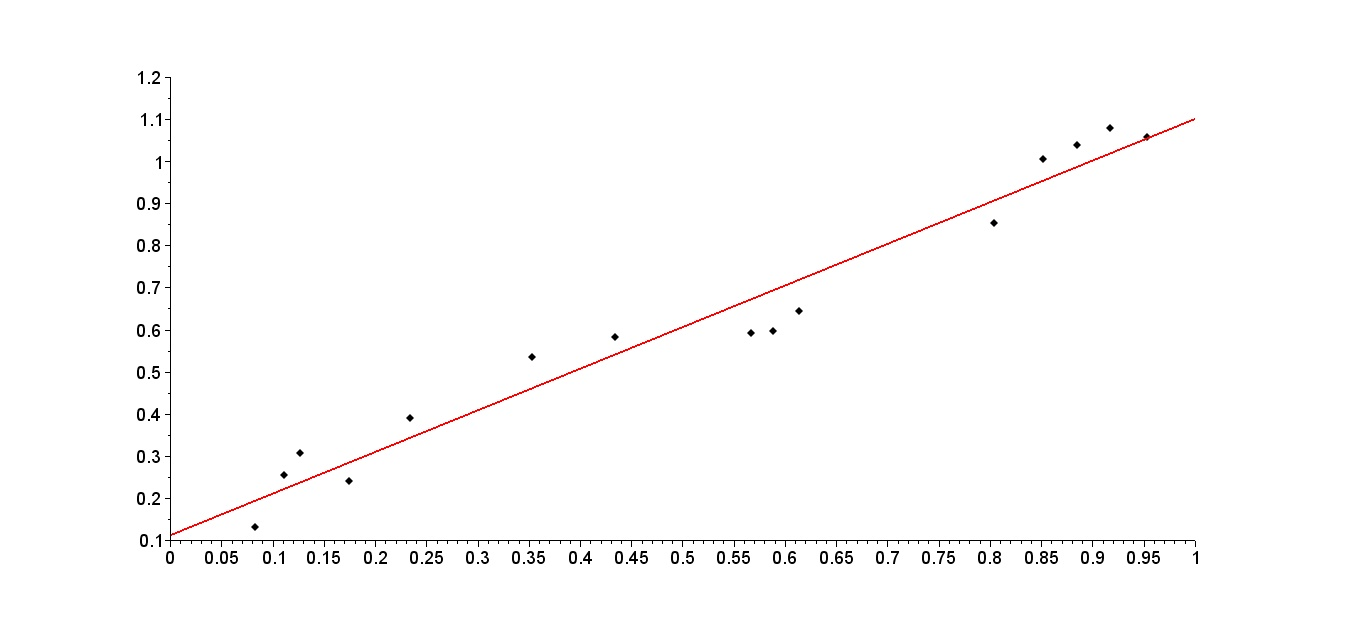
\includegraphics[width=15cm,angle=0]{./cap_aproxfun/pics/ajuste_reta}
{\caption{Conjunto de 15 pontos e a reta que melhor se ajuste a eles pelo critério do mínimos quadrados.}}
\end{center}
\end{figure}

No problema de ajuste de curvas, busca-se a função $f(x)$ de família de funções dadas que melhor se aproxima de um conjunto de pontos dados. O critério mais usado para o ajuste é critério dos mínimos quadrados, ou seja, buscamos a função $f(x)$ da família que minimiza a soma dos erros elevados ao quadrado:
$$E_q=\left[f(x_1)-y_1\right]^2+\left[f(x_2)-y_2\right]^2+\cdots +\left[f(x_n)-y_n\right]^2=\sum_{j=1}^n \left[f(x_j)-y_j\right]^2$$

\begin{ex} Encontre a função do tipo $f(x)=ax$ que melhor se aproxima dos seguintes pontos:
  \begin{equation*}
    (0,-0,1), (1,~2), (2,~3,7) ~ \hbox{e} ~(3,~7).  
  \end{equation*}
\end{ex}
\begin{sol}
Defina $$E_q=[f(x_1)-y_1]^2+[f(x_2)-y_2]^2+[f(x_3)-y_3]^2+[f(x_4)-y_4]^2$$
temos que
\begin{eqnarray*}
E_q&=&[f(0)+0,1]^2+[f(1)-2]^2+[f(2)-3,7]^2+[f(3)-7]^2\\
&=&[0,1]^2+[a-2]^2+[2a-3,7]^2+[3a-7]^2
\end{eqnarray*}

Devemos encontrar o parâmetro $a$ que minimiza o erro, portanto, calculamos:
\begin{eqnarray*}
\frac{\partial E_q}{\partial a}&=&2[a-2]+4[2a-3,7]+6[3a-7]=28a-60,8
\end{eqnarray*}
Portanto o valor de $a$ que minimiza o erro é $a=\frac{60,8}{28}$.
\ifisscilab
\begin{verbatim}
x=[0 1 2 3]'
y=[-.1 2 3.7 7]'
plot2d(x,y,style=-4)
\end{verbatim}
\fi
\end{sol}

\begin{ex}Encontre a função do tipo $f(x)=bx+a$ que melhor aproxima os pontos:
  \begin{equation*}
    (0,-0,1), (1,~2), (2,~3,7) ~ \hbox{e} ~(3,~7).  
  \end{equation*}
\end{ex}
\begin{sol}
\begin{eqnarray*}
E_q&=&[f(0)+0,1]^2+[f(1)-2]^2+[f(2)-3,7]^2+[f(3)-7]^2\\
&=&[a+0,1]^2+[a+b-2]^2+[a+2b-3,7]^2+[a+3b-7]^2
\end{eqnarray*}

Devemos encontrar os parâmetros $a$ $b$ que minimizam o erro, por isso, calculamos as derivadas parciais:
\begin{eqnarray*}
\frac{\partial E_q}{\partial a}&=&2[a+0,1]+2[a+b-2]+2[a+2b-3,7]+2[a+3b-7]\\
\frac{\partial E_q}{\partial b}&=&2[a+b-2]+4[a+2b-3,7]+6[a+3b-7]
\end{eqnarray*}



O erro mínimo acontece quando as derivadas são nulas, ou seja:
\begin{eqnarray*}
8a+12b&=&25,2\\
12a+28b&=&60,8
\end{eqnarray*}
Cuja solução é dada por $a=-0,3$ e $b=2,3$.
Portanto a função que procuramos é $f(x)=-0,3 +2,3x$.  
\end{sol}



\section{O caso linear}

\subsection{O método dos mínimos quadrados}

Considere o sistema linear dado por
$Ax=b$
onde $A$ é uma matriz $n\times m$ e $b$ é um vetor de $n$ linhas. Assumimos as seguintes hipóteses:
\begin{itemize}
\item $n\geq m$. O número de linhas é igual ou superior ao número de colunas. (Mais equações que incógnitas)
\item O posto de $A$ é $m$, i.e., existem $m$ linhas L.I. Isso implica que $Av=0$ apenas quando $v=0$
\end{itemize}

Neste caso, não seremos necessariamente capazes de encontrar um vetor $x$ que satisfaça exatamente a equação $Ax=b$, pelo que estamos interessamos no problema de encontrar o vetor $x$ (ordem m) que minimiza o erro quadrático dado por:
\begin{equation}\label{defEm}
E:=\sum_{i=1}^n \left[z_i- b_i\right]^2
\end{equation}
onde $z=Ax$ e $z_i$ é linha $i$ do vetor $z$, dado por:
\begin{equation}\label{Axi}
z_i=(Ax)_i=\sum_{j=1}^m a_{ij} x_j,\quad i=1,\cdots,n
\end{equation}
onde $a_{ij}$ é o elemento de $A$ na linha $i$ e coluna $j$.
Substituindo (\ref{Axi}) em (\ref{defEm})
\begin{equation}\label{erro}
E:=\sum_{i=1}^n \left[\sum_{j=1}^m a_{ij} x_j- b_i\right]^2
\end{equation}
Esta é uma função diferenciável nos coeficientes $x_j$ e portanto todo ponto de mínimo acontece quando $\nabla E=0$, ou seja, quando $$\frac{\partial}{\partial x_l}E=0,\forall 1\leq l \leq m $$
O que implica a seguinte condição
\begin{eqnarray*}
0=\frac{\partial}{\partial x_l}E=\sum_{i=1}^n 2\left[\sum_{j=1}^m a_{ij} x_j- b_i\right] a_{il}, ~~~l=1,\cdots, m
\end{eqnarray*}
Equivalente a
\begin{eqnarray*}
\sum_{i=1}^n\sum_{j=1}^m  a_{il}x_j a_{ij}=\sum_{i=1}^na_{il}b_i,~~~l=1,\cdots, m
\end{eqnarray*}
que pode ser reescrito na forma vetorial como:
\begin{eqnarray}\label{cond_vet}
\left[
\begin{array}{c}
\sum_{i=1}^n\sum_{j=1}^m   a_{i1}x_ja_{ij}\\
\sum_{i=1}^n\sum_{j=1}^m   a_{i2}x_ja_{ij}\\
\vdots\\
\sum_{i=1}^n\sum_{j=1}^m   a_{im}x_ja_{ij}\\
\end{array}
\right]
=
\left[
\begin{array}{c}
\sum_{i=1}^na_{i1}b_i\\
\sum_{i=1}^na_{i2}b_i\\
\vdots\\
\sum_{i=1}^na_{im}b_i
\end{array}
\right]
\end{eqnarray}
Observamos agora que a expressão (\ref{cond_vet}) é equivalente ao seguinte problema matricial:

\begin{equation}\framebox[100 pt][c]{$A^TA x = A^Tb$}\end{equation}

\begin{teo}
A matriz $M=A^TA$ é quadrada de ordem $m$ e é invertível sempre que o posto da matriz $A$ é igual a número de colunas $m$.
\end{teo}
\begin{proof}
Para provar que $M$ é invertível precisamos mostrar que $Mv=0$ implica $v=0$:
$$Mv=0\Longrightarrow A^TAv=0$$
tomando o produto interno da expressão $0=A^TAv$ com $v$, temos:
$$0=\left<A^TAv,v\right>=\left<Av,Av\right>=\|Av\|^2$$
Então se $Mv=0$ $Av=0$, como o posto de $A$ é igual ao número de colunas, $v=0$.
\end{proof}
Outra propriedade importante é que $M$ é simétrica, ou seja, $M=M^T$. Isso é facilmente provado pelo seguinte argumento:
$$M^T=(A^TA)^T=(A)^T(A^T)^T=A^TA=M$$


\subsection{Ajuste linear de curvas}
Seja $f_1(x), f_2(x),\ldots, f_m(x)$ um conjunto de $m$ funções e $(x_1,y_1), (x_2,y_2), \ldots, (x_n,y_n)$ um conjunto de $n$ pontos. Procuram-se os coeficientes $a_1,a_2,\ldots, a_m$ tais que a função dada por
$$f(x)=a_1f_1(x)+a_2f_2(x)+\ldots+a_mf_m(x)$$
minimiza o erro dado por
$$E_q= \sum_{i=1}^n \left[f(x_i)-y_i\right]^2$$
como $f(x)=\sum_{j=1}^m a_jf_j(x)$, temos
$$E_q= \sum_{i=1}^n \left[\sum_{j=1}^m a_jf_j(x_i)-y_i\right]^2$$

Este problema é equivalente a resolver pelo métodos dos mínimos quadrados o seguinte sistema linear:
$$
\left[
\begin{array}{cccc}
f_1(x_1)&f_2(x_1) & \cdots & f_m(x_1)\\
f_1(x_2)&f_2(x_2) & \cdots & f_m(x_2)\\
f_1(x_3)&f_2(x_3) & \cdots & f_m(x_3)\\
\vdots & \vdots & \ddots & \vdots\\
f_1(x_n)&f_2(x_n) & \cdots & f_m(x_n)
\end{array}
\right]
\left[
\begin{array}{c}
a_1\\
a_2\\
\vdots\\
a_m
\end{array}
\right]=\left[\begin{array}{c}
y_1\\
y_2\\
y_3\\
\vdots\\
y_n
\end{array}
\right]
$$



\begin{ex} Encontre a reta que melhor aproxima o seguinte conjunto de dados:
  \begin{center}
    \begin{tabular}{|c|c|}
      \hline
      $x_i$ & $y_i$\\
      \hline
      $0,01$ & $1,99$\\
      $1,02$ & $4,55$\\
      $2,04$ & $7,20$\\
      $2,95$ & $9,51$\\
      $3,55$ & $10,82$\\
      \hline
    \end{tabular}
  \end{center}
\end{ex}
\begin{sol}
Desejamos então encontrar os valores de $a$ e $b$ tais que a função $f(x)=ax+b$ melhor se ajusta aos pontos da tabela. Afim de usar  o critério dos mínimos quadrados, escrevemos o problema na forma matricial dada por:
$$
\left[\begin{array}{cc}
0,01 &1\\
1,02 &1\\
2,04 &1\\
2,95 &1\\
3,55 &1
\end{array}
\right]
\left[\begin{array}{c}
a\\
b
\end{array}
\right]
=
\left[\begin{array}{c}
1,99\\
4,55\\
7,2\\
9,51\\
10,82
\end{array}
\right]
$$

Multiplicamos agora ambos os lados pela transposta:
\begin{equation*}
\left[\begin{array}{ccccc}
0,01 &1,02 &2,04 &2,95 &3,55\\
1 &1 &1 &1 &1
\end{array}
\right]
\end{equation*}
o que fornece:
\begin{align*}
&\left[\begin{array}{ccccc}
0,01 &1,02 &2,04 &2,95 &3,55\\
1 &1 &1 &1 &1
\end{array}
\right]
\left[\begin{array}{cc}
0,01 &1\\
1,02 &1\\
2,04 &1\\
2,95 &1\\
3,55 &1
\end{array}
\right]
\left[\begin{array}{c}
a\\
b
\end{array}
\right]
=\\
&\left[\begin{array}{ccccc}
0,01 &1,02 &2,04 &2,95 &3,55\\
1 &1 &1 &1 &1
\end{array}
\right]
\left[\begin{array}{c}
1,99\\
4,55\\
7,2\\
9,51\\
10,82
\end{array}
\right]  
\end{align*}
$$\left[
\begin{array}{cc}
26,5071  & 9,57 \\
  9,57  &     5
\end{array}
\right]
\left[
\begin{array}{c}
a   \\
b
\end{array}
\right]=
\left[
\begin{array}{c}
85,8144  \\
34,07
\end{array}
\right]
$$

A solução desse sistema é $a=2,5157653$ e $b=1,9988251$

A tabela abaixo mostra os valores dados e os valores ajustados:
\begin{center}
\begin{tabular}{|c|c|c|c|}
\hline
$x_i$ & $y_i$& $ax_i+b$& $ax_i+b-y_i$\\
\hline
$0,01$ & $1,99$ & $2,0239828$ & $0,0339828$\\
$1,02$ & $4,55$ & $4,5649057$ & $0,0149057$ \\
$2,04$ & $7,2$ & $7,1309863$ & $-0,0690137$ \\
$2,95$ & $9,51$ & $9,4203327$ & $-0,0896673$  \\
$3,55$ & $10,82$ & $10,929792$ & $0,1097919$ \\
\hline
\end{tabular}  
\end{center}
\end{sol}

\section*{Exercícios}

\begin{Exercise}Encontrar  a parábola $y=ax^2+bx+c$ que melhor aproxima o seguinte conjunto de dados:
  \begin{center}
    \begin{tabular}{|c|c|}
      \hline
      $x_i$ & $y_i$\\
      \hline
      $0,01$ & $1,99$\\
      $1,02$ & $4,55$\\
      $2,04$ & $7,2$\\
      $2,95$ & $9,51$\\
      $3,55$ & $10,82$\\
      \hline
    \end{tabular}    
  \end{center}
  e complete a tabela:
  \begin{center}
    \begin{tabular}{|c|c|c|c|}
      \hline
      $x_i$ & $y_i$& $ax_i^2+bx_i+c$& $ax_i^2+bx_i+c-y_i$\\
      \hline
      $0,01$ & $1,99$& &\\
      $1,02$ & $4,55$&& \\
      $2,04$ & $7,20$&  & \\
      $2,95$ & $9,51$  &  & \\
      $3,55$ & $10,82$&&\\
      \hline
    \end{tabular}
  \end{center}
\end{Exercise}
\begin{Answer}
  \begin{tiny}
$y=-0,0407898x^2+ 2,6613293x+ 1,9364598$    
\begin{equation*}
\begin{tabular}{|c|c|c|c|}
\hline
$x_i$ & $y_i$& $ax_i^2+bx_i+c$& $ax_i^2+bx_i+c-y_i$\\
\hline
0,01 & 1,99&1,963069&-0,0269310  \\
1,02 & 4,55&4,6085779&    0,0585779  \\
2,04 & 7,2&7,1958206  &  -0,0041794  \\
2,95 & 9,51& 9,4324077   &-0,0775923   \\
3,55 & 10,82& 10,870125   &0,0501249\\
\hline
\end{tabular}  
\end{equation*}
  \end{tiny}
\end{Answer}


\begin{Exercise} Dado o seguinte conjunto de dados
  \begin{equation*}
    \begin{tabular}{|c|c|}
      \hline
      $x_i$ & $y_i$\\
      \hline
      0,0 &  31\\
      0,1 &  35\\
      0,2 &  37\\
      0,3 &  33\\
      0,4 &  28\\
      0,5 &  20\\
      0,6 &  16\\
      0,7 &  15\\
      0,8 &  18\\
      0,9 &  23\\
      1,0 &  31\\
      \hline
    \end{tabular}    
  \end{equation*}
\begin{itemize}
\item Encontre a função do tipo $f(x)=a+b\sin(2\pi x)+c\cos(2\pi x)$ que melhor aproxima os valores dados.
\item Encontre a função do tipo $f(x)=a+bx+cx^2+dx^3$ que melhor aproxima os valores dados.
\end{itemize}
\end{Exercise}
\begin{Answer}
  \begin{tiny}
      $a=25,638625$, $b=9,8591874$, $c=4,9751219$ e   $a=31,475524$, $b=65,691531$, $c=-272,84382$, $d=208,23621$.
  \end{tiny}
\end{Answer}

\section{Aproximando problemas não lineares por problemas lineares}

Eventualmente, problemas de ajuste de curvas podem recair num sistema não linear. Por exemplo, se desejamos ajustar a função $y=Ae^{bx}$ ao conjunto de pontos $(x_0,y_0)$, $(x_1,y_1)$ e $(x_2,y_2)$, temos que minimizar o funcional
$$
E_q=(Ae^{x_0b}-y_0)^2+(Ae^{x_1b}-y_1)^2+(Ae^{x_2b}-y_2)^2
$$
ou seja, resolver o sistema
\begin{align*}
\frac{\partial E_q}{\partial A} &= 2(Ae^{x_0b}-y_0)e^{x_0b}+2(Ae^{x_1b}-y_1)e^{x_1b}+2(Ae^{x_2b}-y_2)e^{x_2b}=0\\
\frac{\partial E_q}{\partial b} &= 2Ax_0(Ae^{x_0b}-y_0)e^{x_0b} + 2Ax_1(Ae^{x_1b}-y_1)e^{x_1b} \\
&+ 2x_2A(Ae^{x_2b}-y_2)e^{x_2b}=0
\end{align*}
que é não linear em $A$ e $b$. Esse sistema pode ser resolvido pelo método de Newton-Raphson, o que pode se tornar custoso, ou mesmo inviável quando não dispomos de uma boa aproximação da solução para inicializar o método.

Felizmente, algumas famílias de curvas admitem uma transformação que nos leva a um problema linear. No caso da curva $y=Ae^{bx}$, observe que $\ln y=\ln A+bx$. Assim, em vez de ajustar a curva original $y=Ae^{bx}$ a tabela de pontos, ajustamos a curva submetida a transformação logarítmica
$$
z=\ln A+bx:=B+bx.
$$
Usamos os três pontos $(x_0,\ln y_0):=(x_0, \tilde{y}_0)$, $(x_1,\ln y_1):=(x_1,\tilde{y}_1)$ e $(x_2,\ln y_2):=(x_2,\tilde{y}_2)$ e resolvemos o sistema linear
$$
A^T A \left[\begin{array}{c} B\\b \end{array}\right]=A^T\left[\begin{array}{c}\tilde{y}_0\\\tilde{y}_1\\\tilde{y}_2 \end{array}\right],
$$
onde
$$
A=\left[\begin{array}{cc} 1&x_0\\1&x_1\\1&x_2 \end{array}\right]
$$
\begin{ex}Encontre uma curva da forma $y=Ae^x$ que melhor ajusta os pontos $(1,2)$, $(2,3)$ e $(3,5)$.
\end{ex}
Temos
$$
A=\left[\begin{array}{cc} 1&1\\1&2\\1&3 \end{array}\right]
$$
e a solução do sistema leva em $B=0,217442$ e $b=0,458145$. Portanto, $A=e^{0,217442}=1,24289$.

\begin{obs}
Os coeficientes obtidos a partir dessa linearização são aproximados, ou seja, são diferentes daqueles obtidos quando aplicamos mínimos quadrados não linear. Observe que estamos minimizando $\displaystyle\sum_i [\ln y_i -\ln (f(x_i))]^2$ em vez de $\displaystyle\sum_i [ y_i -f(x_i)]^2$. No exemplo resolvido, a solução do sistema não linear original seria $A=1,19789$ e $B=0,474348$
\end{obs}

\begin{obs}
Mesmo quando se deseja resolver o sistema não linear, a solução do problema linearizado pode ser usada para construir condições iniciais.
\end{obs}


A próxima tabela apresenta algumas curvas e transformações que linearizam o problema de ajuste.
$$
\begin{array}{|c|c|c|}
\hline
\hbox{curva}&\hbox{transformação}&\hbox{problema linearizado}\\
\hline
y=ae^{bx}&Y=\ln y&Y=\ln a+ bx\\
\hline
y=ax^b&Y=\ln y&Y=\ln a+ b\ln x\\
\hline
y=ax^be^{cx}&Y=\ln y&Y=\ln a+ b\ln x+cx\\
\hline
y=ae^{(b+cx)^2}&Y=\ln y&Y=\ln a+b^2+ bc x+c^2x^2\\
\hline
y=\frac{a}{b+x}&Y=\frac{1}{y}&Y=\frac{b}{a}+\frac{1}{a}x\\
\hline
\begin{array}{c}y=A\cos(\omega x+\phi)\\ \omega\ \hbox{conhecido}\end{array}&-&\begin{array}{c}y=a\cos(\omega x)-b\sin(\omega x),\\a=A\cos(\phi),\ b=A\sin(\phi)\end{array}\\
\hline
\end{array}
$$

\begin{ex}
Encontre a função $f$ da forma $y=f(x)=A\cos(2 \pi x+\phi)$ que ajusta a tabela de pontos
$$
\begin{tabular}{|c|c|}
\hline
$x_i$ & $y_i$\\
\hline
0,0  &   9,12\\
0,1  &    1,42\\
0,2  &  - 7,76\\
0,3  &  - 11,13\\
0,4  &  - 11,6\\
0,5  &  - 6,44\\
0,6  &    1,41\\
0,7  &    11,01\\
0,8  &    14,73\\
0,9  &    13,22\\
1,0  &    9,93 \\
\hline
\end{tabular}
$$
\end{ex}
\begin{sol}
Usando o fato que $y=A\cos(2 \pi x+\phi)=a\cos(2 \pi x)-b\sin(2 \pi x)$, onde $a=A\cos(\phi)$ e $b=A\sin(\phi)$, $z=[\begin{array}{cc}a &b\end{array}]^T$ é solução do problema
$$
B^TBz=B^Ty,
$$
onde
$$
B\!=\!\left[\begin{array}{cc}\cos(2 \pi x_0)& -\sin(2 \pi x_0)\\ \cos(2 \pi x_1)& -\sin(2 \pi x_1)\\ \vdots\\ \cos(2 \pi x_{10})& -\sin(2\pi x_{10}) \end{array}\right]\!=\!\left[\begin{array}{cc}  1.     &      0.\\
    0,8090170 & - 0,5877853\\
    0,3090170 & - 0,9510565\\
  - 0,3090170 & - 0,9510565\\
  - 0,8090170 & - 0,5877853\\
  - 1,0000000 &   0,0000000\\
  - 0,8090170 &   0,5877853\\
  - 0,3090170 &   0,9510565\\
    0,3090170 &   0,9510565\\
    0,8090170 &   0,5877853\\
    1,0000000 &   0,0000000   \end{array}\right].
$$
Assim, $a=7,9614704$ e $b=11,405721$ e obtemos o seguinte sistema:
$$
\left\{\begin{array}{c}
A\cos(\phi)=7,9614704\\ A\sin(\phi)=11,405721
\end{array}\right..
$$
Observe que
$$
A^2=7,9614704^2+11,405721^2
$$
e, escolhendo $A>0$, $A=13,909546$ e
$$
\sin(\phi)=\frac{11,405721}{13,909546}=0,8199923
$$
Assim, como $\cos\phi$ também é positivo, $\phi$ é um ângulo do primeiro quadrante:
$$
\phi=0,9613976
$$
Portanto $f(x)=13,909546\cos(2\pi x+0,9613976)$. Observe que nesse exemplo a solução do problema linear é a mesma do problema não linear.  
\end{sol}

\begin{ex}
Encontre a função $f$ da forma $y=f(x)=\frac{a}{b+x}$ que ajusta a tabela de pontos
$$
\begin{tabular}{|c|c|}
\hline
$x_i$ & $y_i$\\
\hline
0,0  & 101\\
0,2  &  85\\
0,4  &  75\\
0,6  &  66\\
0,8  &  60\\
1,0  &  55 \\
\hline
\end{tabular}
$$
usando uma das transformações tabeladas.
\end{ex}
\begin{sol}
Usando o fato que $Y=\frac{1}{y}=\frac{b}{a}+\frac{1}{a}x$, $z=[\begin{array}{cc}\frac{b}{a} &\frac{1}{a}\end{array}]^T$ é solução do problema
$$
A^TAz=A^TY,
$$
onde
$$
A=\left[\begin{array}{cc}1& x_1\\ 1& x_2\\ 1&x_3\\1&x_4 \\ 1&x_5 \\ 1&x_6 \end{array}\right]=\left[\begin{array}{cc}
  1 &  0,0\\
  1 &  0,2\\
  1 &  0,4\\
  1 &  0,6\\
  1 &  0,8\\
  1 &  1,0
\end{array}\right]
$$
e
$$
Y=\left[\begin{array}{c}
  1/y_1\\
    1/y_2\\
    1/y_3\\
    1/y_4\\
    1/y_5\\
    1/y_6
\end{array}\right]=\left[\begin{array}{c}
  0,0099010\\
  0,0117647\\
  0,0133333\\
  0,0151515\\
  0,0166667\\
  0,0181818
\end{array}\right]
$$
Assim, $\frac{1}{a}=0,0082755$ e $\frac{b}{a}=0,0100288$ e, então, $a=120,83924$ e $b=1,2118696$, ou seja, $f(x)=\frac{120,83924}{1,2118696+x}$.  
\end{sol}


\section{Interpolação linear segmentada}\index{interpolação!linear segmentada}
Considere o conjunto $\left(x_i,y_i\right)_{j=1}^n$ de $n$ pontos. Assumiremos que $x_{i+1}>x_i$, ou seja, as abscissas são distintas e estão em ordem crescente. A função linear que interpola os pontos $x_i$ e $x_{i+1}$ no intervalo $i$ é dada por
$$P_i(x)=y_i \frac{(x_{i+1}-x)}{(x_{i+1}-x_i)} + y_{i+1} \frac{(x-x_i)}{(x_{i+1}-x_i)}$$

O resultado da interpolação linear segmentada é a seguinte função contínua definida por partes no intervalo $[x_1,x_n]$:
$$f(x)=P_i(x), ~~~~ x\in [x_i,x_{i+1}]$$

\begin{ex}
  Construa uma função linear por partes que interpola os pontos $(0,0)$, $(1,4)$, $(2,3)$, $(3,0)$, $(4,2)$, $(5,0)$.

A função procurada pode ser construída da seguinte forma:
\begin{equation*}
  f(x) = \left\{
    \begin{array}{ll}
      0\frac{x-1}{0-1} + 1\frac{x-0}{1-0} &, 0 \leq x < 1\\
      4\frac{x-2}{1-2} + 3\frac{x-1}{2-1} &, 1\leq x < 2\\
      3\frac{x-3}{2-3} + 0\frac{x-2}{3-2} &, 2\leq x \leq 3
    \end{array}
\right.
\end{equation*}
Simplificando, obtemos:
\begin{equation*}
  f(x) = \left\{
    \begin{array}{ll}
      x &, 0 \leq x < 1\\
      -x + 5 &, 1\leq x < 2\\
      -3x + 9 &, 2\leq x \leq 3
    \end{array}
\right.  
\end{equation*}
\end{ex}

A Figura \ref{fig:linear_segmentada} é um esboço da função $f(x)$ obtida. 
\ifisscilab
Ela foi gerada no \verb+Scilab+ usando os comandos:
\verbatiminput{./cap_aproxfun/codes/interpolacao_linear_segmentada/ex_linear_segmentada.sce}
\fi

\begin{figure}[htp]
\begin{center}
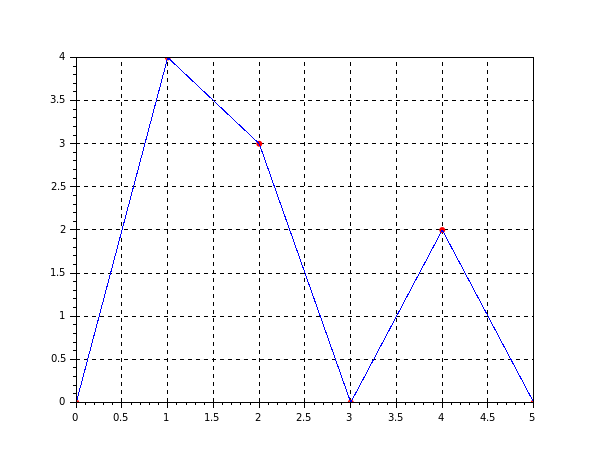
\includegraphics[scale=0.5]{./cap_aproxfun/pics/interpolacao_linear_segmentada.png}
\caption{Interpolação linear segmentada.}
\label{fig:linear_segmentada}
\end{center}
\end{figure}


\section{Interpolação cúbica segmentada - spline}\index{interpolação!cúbica segmentada}\index{spline}
Dado um conjunto de $n$ pontos $\left(x_j,y_j\right)_{j=1}^n$ tais que $x_{j+1}>x_j$, ou seja, as abscissas são distintas e estão em ordem crescente; um spline cúbico que interpola estes pontos é uma função $s(x)$ com as seguintes propriedades:
\begin{itemize}
\item[i] Em cada segmento $[x_j,x_{j+1}]$, $j=1,2,\ldots n-1$ $s(x)$ é um polinômio cúbico.
\item[ii] para cada ponto, $s(x_j)=y_j$, i.e., o spline interpola os pontos dados.
\item[iii] $s(x)\in C^2$, i.e., é função duas vezes continuamente diferenciável.
\end{itemize}

Da primeira hipótese, escrevemos
$$s(x)=s_j(x),x \in [x_j,x_{j+1}],~~ j=1,\ldots, n-1$$
com
$$s_j(x)=a_j+b_j(x-x_j)+c_j(x-x_j)^2+d_j(x-x_j)^3$$
O problema agora consiste em obter os 4 coeficientes de cada um desses $n-1$ polinômios cúbicos.

Veremos que a simples definição de spline produz $4n-6$ equações linearmente independentes:
\begin{equation*}
\begin{array}{rcll}
s_j(x_j)&=&y_j,~~ &j=1,\ldots, n-1\\
s_{j}(x_{j+1})&=&y_{j+1},~~ &j=1,\ldots, n-1\\
s_{j}'(x_{j+1})&=&s_{j+1}'(x_{j+1}),~~ &j=1,\ldots, n-2\\
s_{j}''(x_{j+1})&=&s_{j+1}''(x_{j+1}),~~ &j=1,\ldots, n-2
\end{array}
\end{equation*}
Como
\begin{equation}{\label{eq_1derivada}}
s'_j(x)=b_j+2c_j(x-x_j)+3d_j(x-x_j)^2
\end{equation}
e
\begin{equation}{\label{eq_2derivada}}
s''_j(x)=2c_j+6d_j(x-x_j),
\end{equation}
temos, para $j=1,\ldots, n-1$, as seguintes equações
\begin{equation*}
\begin{array}{rcl}
a_j&=&y_j,\\
a_j+b_j(x_{j+1}-x_j)+c_j(x_{j+1}-x_j)^2+d_j(x_{j+1}-x_j)^3&=&y_{j+1},\\
b_j+2c_j(x_{j+1}-x_j)+3d_j(x_{j+1}-x_j)^2&=&b_{j+1},\\
c_j+3d_j(x_{j+1}-x_j)&=&c_{j+1},
\end{array}
\end{equation*}
Por simplicidade, definimos
$$
h_j=x_{j+1}-x_j
$$
e temos
\begin{equation}
\begin{array}{rcl}
a_j&=&y_j,\\
a_j+b_jh_j+c_jh_j^2+d_jh_j^3&=&y_{j+1},\\
{\label{eq3}}b_j+2c_jh_j+3d_jh_j^2&=&b_{j+1},\\
\nonumber c_j+3d_jh_j&=&c_{j+1},
\end{array}
\end{equation}
que podem ser escrita da seguinte maneira
\begin{equation}{\label{eq_an_spline}}
a_j=y_j,
\end{equation}
\begin{equation}{\label{eq_dn_spline}}
d_j=\frac{c_{j+1}-c_j}{3h_j},
\end{equation}
\begin{eqnarray}
\nonumber b_j&=&\frac{y_{j+1}-y_j-c_jh_j^2-\frac{c_{j+1}-c_j}{3h_j}h_j^3}{h_j},\\
\nonumber &=&\frac{3y_{j+1}-3y_j-3c_jh_j^2-c_{j+1}h_j^2+c_jh_j^2}{3h_j}\\
{\label{eq_bn_spline}}&=&\frac{3y_{j+1}-3y_j-2c_jh_j^2-c_{j+1}h_j^2}{3h_j}
\end{eqnarray}
Trocando o índice $j$ por $j-1$ na terceira equação (\ref{eq3}), $j=2,\ldots, n-1$
\begin{equation}
b_{j-1}+2c_{j-1}h_{j-1}+3d_{j-1}h_{j-1}^2=b_{j}  
\end{equation}
e, portanto,
\begin{equation}
  \begin{split}
    \frac{3y_{j}-3y_{j-1}-2c_{j-1}h_{j-1}^2-c_{j}h_{j-1}^2}{3h_{j-1}} &+ 2c_{j-1}h_{j-1}+c_{j}h_{j-1}-c_{j-1}h_{j-1} \\
    &=\frac{3y_{j+1}-3y_j-2c_jh_j^2-c_{j+1}h_j^2}{3h_j}.      
  \end{split}
\end{equation}
Fazendo as simplificações, obtemos:
\begin{equation}{\label{eq_cn_spline}}
c_{j-1}h_{j-1}+c_j(2h_j+2h_{j-1})+c_{j+1}h_j=3\frac{y_{j+1}-y_j}{h_j}-3\frac{y_{j}-y_{j-1}}{h_{j-1}}.
\end{equation}
É costumeiro acrescentar a incógnita $c_n$ ao sistema. A incógnita $c_n$ não está relacionada a nenhum dos polinômios interpoladores. Ela é uma construção artificial que facilita o cálculo dos coeficientes do spline. Portanto, a equação acima pode ser resolvida para $j=2, \ldots, n-1$.

Para determinar unicamente os $n$ coeficientes $c_n$ precisamos acrescentar duas equações linearmente independentes às $n-2$ equações dadas por (\ref{eq_cn_spline}). Essas duas equações adicionais definem o tipo de spline usado.

\subsection{Spline natural}\index{spline!natural}

Uma forma de definir as duas equações adicionais para completar o sistema (\ref{eq_cn_spline}) é impor condições de fronteira livres (ou naturais), ou seja,
\begin{equation}
S''(x_1)=S''(x_n)=0.
\end{equation}
Substituindo na equação (\ref{eq_2derivada})
$$
s''_1(x_1)=2c_1+6d_1(x_1-x_1)=0 \Longrightarrow c_1=0.
$$
e
$$
s''_{n-1}(x_n)=2c_{n-1}+6d_{n-1}(x_{n}-x_{n-1})=0 .
$$
Usando o fato que
$$
c_{n-1}+3d_{n-1}h_{n-1}=c_{n}
$$
temos que
$$
c_n=-3d_{n-1}(x_{n}-x_{n-1})+3d_{n-1}h_{n-1}=0.
$$
Essa duas equações para $c_1$ e $c_n$ juntamente com as equações (\ref{eq_cn_spline}) formam um sistema de $n$ equações $Ac=z$, onde
\begin{equation}
A=\left[\begin{array}{ccccccc}
1 &0&0&0 &\cdots&0&0\\
h_1&2h_2+2h_{1}&h_2&0&\cdots&0&0\\
0&h_2&2h_3+2h_{2}&h_3&\cdots&0&0\\
\vdots&\vdots&\vdots&\vdots&\ddots&\vdots&\vdots\\
0&0&0&\cdots&h_{n-2} & 2h_{n-2}+2h_{n-1}&h_{n-1}\\
0&0&0&\cdots &0&0&1
\end{array}\right]  
\end{equation}
\begin{equation}
c = \left[\begin{array}{c}
c_1\\
c_2\\
\vdots\\
c_n
\end{array}\right]\qquad \hbox{e}\qquad
z = \left[\begin{array}{c}
0\\
3\frac{y_{3}-y_2}{h_2}-3\frac{y_{2}-y_{1}}{h_{1}}\\
3\frac{y_{4}-y_3}{h_3}-3\frac{y_{3}-y_{2}}{h_{2}}\\
\vdots\\
3\frac{y_{n-1}-y_{n-2}}{h_{n-2}}-3\frac{y_{n-2}-y_{n-3}}{h_{n-3}}\\
0
\end{array}\right]
\end{equation}
Observe que a matriz $A$ é diagonal dominante estrita e, portanto, o sistema $Ac=z$ possui solução única. Calculado $c$, os valores dos $a_n$, $b_n$ e $d_n$ são obtidos diretamente pelas expressões (\ref{eq_an_spline}), (\ref{eq_bn_spline}) e (\ref{eq_dn_spline}), respectivamente.

\begin{ex}Construa um spline cúbico natural que passe pelos pontos $(2,~4,5)$, $(5,-1,9)$, $(9,~0,5)$ e $(12,-0,5)$.
\end{ex}
\begin{sol}
O spline desejado é uma função definida por partes da forma:
\begin{equation}
f(x)=\left\{\begin{array}{ll}
a_1+b_1(x-2)+c_1(x-2)^2+d_1(x-2)^3 &, 2\leq x <5\\
a_2+b_2(x-5)+c_2(x-5)^2+d_2(x-5)^3 &, 5\leq x <9\\
a_3+b_3(x-9)+c_3(x-9)^2+d_3(x-9)^3 &, 9\leq x \leq 12
\end{array}\right..  
\end{equation}
Os coeficientes $c_1$, $c_2$ e $c_3$ resolvem o sistema $Ac = z$, onde
$$
A=\left[\begin{array}{cccc}
1 &0&0&0 \\
3&2\cdot 3+2\cdot 4&4&0\\
0&4&2\cdot 4+2\cdot 3&3\\
0&0&0&1
\end{array}\right]=\left[\begin{array}{cccc}
1 &0&0&0 \\
3&14&4&0\\
0&4&14&3\\
0&0&0&1
\end{array}\right]
$$
$$
c = \left[\begin{array}{c}
c_1\\
c_2\\
c_3\\
c_4
\end{array}\right]\qquad \hbox{e}\qquad
z=\left[\begin{array}{c}
0\\
3\frac{0,5-(-1,9)}{4}-3\frac{(-1,9)-4,5}{3}\\
3\frac{-0,5-0,5}{3}-3\frac{0,5-(-1,9)}{4}\\
0
\end{array}\right]=\left[\begin{array}{c}
0\\
8,2\\
-2,8\\
0
\end{array}\right]
$$
Observe que $c_4$ é um coeficiente artificial para o problema. A solução é  $c_1=0$, $c_2=0,7$, $c_3=-0,4$ e $c_4=0$. Calculamos os demais coeficientes usando as expressões (\ref{eq_an_spline}), (\ref{eq_bn_spline}) e (\ref{eq_dn_spline}):
\begin{eqnarray*}
a_1&=&y_1=4,5\\
a_2&=&y_2=-1,9\\
a_3&=&y_3=0,5\\
\end{eqnarray*}
\begin{eqnarray*}
d_1&=&\frac{c_{2}-c_1}{3h_1}=\frac{0,7-0}{3\cdot 3}=0,0777778\\
d_2&=&\frac{c_{3}-c_2}{3h_2}=\frac{-0,4-0,7}{3\cdot 4}=-0,0916667\\
d_3&=&\frac{c_{4}-c_3}{3h_3}=\frac{0+0,4}{3\cdot 3}=0,0444444
\end{eqnarray*}
\begin{align*}
b_1 &= \frac{y_{2}-y_1}{h_1}-\frac{h_1}{3}(2c_1+c_{2})\\
&= \frac{-1,9-4,5}{3}-\frac{3}{3}(2\cdot 0-0,7)=-2,8333333\\
b_2&= \frac{y_{3}-y_2}{h_2}-\frac{h_2}{3}(2c_2+c_{3})\\
&= \frac{0,5-(-1,9)}{4}-\frac{4}{3}(2\cdot 0,7+0,4)=-0,7333333\\
b_3&= \frac{y_{4}-y_3}{h_3}-\frac{h_3}{3}(2c_3+c_{4})\\
&= \frac{-0,5-0,5}{3}-\frac{3}{3}(2\cdot (-0,4)+0)=0,4666667
\end{align*}
Portanto:
\begin{small}
\begin{equation*}
f(x)=\left\{\begin{array}{ll}
4,5-2,833(x-2)+0,078(x-2)^3 &\!, 2\leq x<5\\
-1,9-0,733(x-5)+0,7(x-5)^2-0,092(x-5)^3 &\!, 5\leq x<9\\
0,5+0,467(x-9)-0,4(x-9)^2+0,044(x-9)^3 &\!, 9\leq x\leq 12
\end{array}\right.
\end{equation*}  
\end{small}

\ifisscilab
No \verb+Scilab+, podemos utilizar:
\begin{verbatim}
X = [2 5 9 12]'
Y = [4.5 -1.9 0.5 -0.5]'
h = X(2:4)-X(1:3)
A = [1 0 0 0;h(1) 2*h(1)+2*h(2) h(2) 0; ...
   0 h(2) 2*h(2)+2*h(3) h(3);0 0 0 1 ]
z = [0, 3*(Y(3)-Y(2))/h(2)-3*(Y(2)-Y(1))/h(1), ...
   3*(Y(4)-Y(3))/h(3)-3*(Y(3)-Y(2))/h(2), 0]'
c = A\z
for i=1:3
   a(i) = Y(i)
   d(i) = (c(i+1)-c(i))/(3*h(i))
   b(i) = (Y(i+1)-Y(i))/h(i)-h(i)/3*(2*c(i)+c(i+1))
end

for i=1:3
    P(i) = poly([a(i) b(i) c(i) d(i)],'x','coeff')
    z = [X(i):.01:X(i+1)]
    plot(z,horner(P(i),z-X(i)))
end
\end{verbatim}
\fi
\end{sol}

\subsection{Spline fixado}\index{spline!fixado}

Alternativamente, para completar o sistema (\ref{eq_cn_spline}), podemos impor condições de contorno fixadas, ou seja,
\begin{eqnarray*}
S'(x_1)&=&f'(x_1)\\
S'(x_n)&=&f'(x_n).
\end{eqnarray*}
Substituindo na equação (\ref{eq_1derivada})
\begin{equation}
s'_1(x_1)=b_1+2c_1(x_1-x_1)+3d_j(x_1-x_1)^2=f'(x_1)\Longrightarrow b_1=f'(x_1)  
\end{equation}
e
\begin{equation}
  \begin{split}
s'_{n-1}(x_n) &= b_{n-1}+2c_{n-1}(x_n-x_{n-1})+3d_j(x_n-x_{n-1})^2 \\
&= b_{n-1}+2c_{n-1}h_{n-1}+3d_{n-1}h_{n-1}^2=f'(x_n)
  \end{split}
\end{equation}
Usando as equações (\ref{eq_dn_spline}) e (\ref{eq_bn_spline}) para $j=1$ e $j=n-1$, temos:
\begin{equation}
2c_1h_1+c_{2}h_1=3\frac{y_{2}-y_1}{h_1}-3f'(x_1)  
\end{equation}
e
\begin{equation}
c_{n-1}h_{n-1}+c_{n}h_{n-1}=3f'(x_n)-3\frac{y_{n}-y_{n-1}}{h_{n-1}}  
\end{equation}

Essas duas equações juntamente com as equações (\ref{eq_cn_spline}) formam um sistema de $n$ equações $Ac = z$, onde
\begin{equation*}
A=\left[\begin{array}{ccccccc}
2h_1 &h_1&0&0 &\cdots&0&0\\
h_1&2h_2+2h_{1}&h_2&0&\cdots&0&0\\
0&h_2&2h_3+2h_{2}&h_3&\cdots&0&0\\
\vdots&\vdots&\vdots&\vdots&\ddots&\vdots&\vdots\\
0&0&0&\cdots&h_{n-2} & 2h_{n-2}+2h_{n-1}&h_{n-1}\\
0&0&0&\cdots &0&h_{n-1}&2h_{n-1}
\end{array}\right]  
\end{equation*}  
\begin{equation*}
c = \left[\begin{array}{c}
c_1\\
c_2\\
\vdots\\
c_n
\end{array}\right]\qquad \hbox{e}\qquad
z = \left[\begin{array}{c}
3\frac{y_{2}-y_1}{h_1}-3f'(x_1)\\
3\frac{y_{3}-y_2}{h_2}-3\frac{y_{2}-y_{1}}{h_{1}}\\
3\frac{y_{4}-y_3}{h_3}-3\frac{y_{3}-y_{2}}{h_{2}}\\
\vdots\\
3\frac{y_{n-1}-y_{n-2}}{h_{n-2}}-3\frac{y_{n-2}-y_{n-3}}{h_{n-3}}\\
3f'(x_n)-3\frac{y_{n}-y_{n-1}}{h_{n-1}}
\end{array}\right]  
\end{equation*}
Observe que a matriz $A$ é diagonal dominante estrita e, portanto, o sistema $Ac = z$ possui solução única. Calculado $c$, os valores dos $a_n$, $b_n$ e $d_n$ são obtidos diretamente pelas expressões (\ref{eq_an_spline}), (\ref{eq_bn_spline}) e (\ref{eq_dn_spline}), respectivamente.


\begin{ex}Construa um spline cúbico com fronteira fixada que interpola a função $y=\sin (x)$ nos pontos $x=0$, $x=\frac{\pi}{2}$, $x=\pi$, $x=\frac{3\pi}{2}$ e $x=2\pi$.
\end{ex}
O spline desejado passa pelos pontos $(0,0)$, $(\pi/2,1)$, $(\pi,0)$, $(3\pi/2,-1)$ e $(2\pi,0)$ e tem a forma:
\begin{equation*}
f(x)=\left\{\begin{array}{ll}
a_1+b_1x+c_1x^2+d_1x^3&, 0\leq x<\frac{\pi}{2}\\
a_2+b_2(x-\frac{\pi}{2})+c_2(x-\frac{\pi}{2})^2+d_2(x-\frac{\pi}{2})^3&, \frac{\pi}{2}\leq x<\pi\\
a_3+b_3(x-\pi)+c_3(x-\pi)^2+d_3(x-\pi)^3&, \pi\leq x<\frac{3\pi}{2}\\
a_4+b_4(x-\frac{3\pi}{2})+c_4(x-\frac{3\pi}{2})^2+d_4(x-\frac{3\pi}{2})^3&, \frac{3\pi}{2}\leq x\leq 2\pi
\end{array}\right..  
\end{equation*}
Observe que ele satisfaz as condição de contorno $f'(0)=cos(0)=1$ e $f'(2\pi)=cos(2\pi)=1$.

Os coeficientes $c_1$, $c_2$, $c_3$ e $c_4$ resolvem o sistema $Ac = z$, onde:
\begin{equation*}
A=\left[\begin{array}{ccccc}
\pi &\pi/2&0&0&0 \\
\pi/2&2\pi&\pi/2&0&0\\
0&\pi/2&2\pi&\pi/2&0\\
0&0&\pi/2&2\pi&\pi/2\\
0&0&0&\pi/2&\pi\\
\end{array}\right]  
\end{equation*}
\begin{equation*}
c = \left[\begin{array}{c}
c_1\\
c_2\\
c_3\\
c_4\\
c_5
\end{array}\right]\qquad \hbox{e}\qquad
z = \left[\begin{array}{c}
3\frac{1-0}{\pi/2}-3\cdot 1\\
3\frac{0-1}{\pi/2}-3\frac{1-0}{\pi/2}\\
3\frac{-1-0}{\pi/2}-3\frac{0-1}{\pi/2}\\
3\frac{0-(-1)}{\pi/2}-3\frac{(-1)-0}{\pi/2}\\
3\cdot 1-3\frac{0-(-1)}{\pi/2}
\end{array}\right]=\left[\begin{array}{c}
6/\pi-3\\
-12/\pi\\
0\\
12/\pi\\
3-6/\pi
\end{array}\right]  
\end{equation*}
Aqui $c_5$ é um coeficiente artificial para o problema. A solução é  $c_1=-0,0491874$, $c_2=-0,5956302$, $c_3=0$, $c_4=0,5956302$ e $c_5=0,0491874$. Calculamos os demais coeficientes usando as expressões (\ref{eq_an_spline}), (\ref{eq_bn_spline}) e (\ref{eq_dn_spline}):
\begin{eqnarray*}
a_1&=&y_1=0\\
a_2&=&y_2=1\\
a_3&=&y_3=0\\
a_4&=&y_3=-1\\
\end{eqnarray*}
\begin{eqnarray*}
d_1&=&\frac{c_{2}-c_1}{3h_1}=\frac{-0,5956302-(-0,0491874)}{3\cdot \pi/2}=-0,1159588\\
d_2&=&\frac{c_{3}-c_2}{3h_2}=\frac{0-(-0,5956302)}{3\cdot \pi/2}=0,1263967\\
d_3&=&\frac{c_{4}-c_3}{3h_3}=\frac{0,5956302- 0}{3\cdot \pi/2}=0,1263967\\
d_4&=&\frac{c_{5}-c_4}{3h_4}=\frac{0,0491874- 0,5956302}{3\cdot \pi/2}=-0,1159588
\end{eqnarray*}
\begin{align*}
b_1&= \frac{y_{2}-y_1}{h_1}-\frac{h_1}{3}(2c_1+c_{2})\\
&=\frac{1-0}{\pi/2}-\frac{\pi/2}{3}(2\cdot (-0,0491874)-0,5956302)=1\\
b_2&=\frac{y_{3}-y_2}{h_2}-\frac{h_2}{3}(2c_2+c_{3})\\
&=\frac{0-1}{\pi/2}-\frac{\pi/2}{3}(2\cdot(-0,5956302) +0)=-0,0128772\\
b_3&=\frac{y_{4}-y_3}{h_3}-\frac{h_3}{3}(2c_3+c_{4})\\
&=\frac{-1-0}{\pi/2}-\frac{\pi/2}{3}(2\cdot 0+0,5956302)=-0,9484910\\
b_4&=\frac{y_{5}-y_4}{h_4}-\frac{h_4}{3}(2c_4+c_{5})\\
&=\frac{0-(-1)}{\pi/2}-\frac{\pi/2}{3}(2\cdot 0,5956302+0,0491874)=-0,0128772
\end{align*}
Portanto,
\begin{small}
\begin{equation*}
f(x)=\left\{\begin{array}{ll}
x-0,049x^2-0,12x^3&, 0\leq x<\frac{\pi}{2}\\
1+-0,01(x-\frac{\pi}{2})-0,6(x-\frac{\pi}{2})^2+0,13(x-\frac{\pi}{2})^3&, \frac{\pi}{2}\leq x<\pi\\
-0,95(x-\pi)+0,13(x-\pi)^3&, \pi\leq x<\frac{3\pi}{2}\\
-1-0,01(x-\frac{3\pi}{2})+0,6(x-\frac{3\pi}{2})^2-0,12(x-\frac{3\pi}{2})^3&, \frac{3\pi}{2}\leq x\leq2\pi
\end{array}\right.
\end{equation*}  
\end{small}

\ifisscilab
No \verb+Scilab+, podemos resolver este problema fazendo:
\verbatiminput{./cap_aproxfun/codes/splines/ex_spline_fixado.sce}
\fi

\subsubsection{Resumo sobre Splines}

Dado um conjunto de pontos $(x_i,y_i)$, $i=1,2,\ldots,n$, um spline cúbico é a seguinte função definida por partes:
\begin{small}
\begin{equation*}
  s(x) \!=\! \left\{\begin{array}{ll}
       \!\!\!a_1 \!+\! b_1(x\!-\!x_1) \!+\! c_1(x\!-\!x_1)^2 \!+\! d_1(x\!-\!x_1)^3 &\!\!\!\!\!, x_1\leq x < x_2\\
      \!\!\!a_2 \!+\! b_2(x\!-\!x_2) \!+\! c_2(x\!-\!x_2)^2 \!+\! d_2(x\!-\!x_2)^3 &\!\!\!\!\!, x_2 \leq x < x_3\\
      \qquad\qquad \vdots & \qquad\vdots \\
      \!\!\!a_{n-1} \!+\! b_{n-1}(x\!-\!x_{n-1}) \!+\! c_{n-1}(x\!-\!x_{n-1})^2 \!+\! d_{n-1}(x\!-\!x_{n-1})^3 &\!\!\!\!\!, x_{n-1} \leq x \leq x_n \end{array}\right.
\end{equation*}  
\end{small}

Definindo-se $h_j = x_{j+1} - x_j$, os coeficientes $c_j$, $j=1,2,\dotsc,n$, são solução do sistema linear $Ac = z$, onde:
\begin{small}
  \begin{equation*}
  \begin{array}{|l|l|}\hline
    \text{Spline Natural} & \text{Spline Fixado}\\
    s_1''(x_1) = 0 \text{ e } s_{n-1}''(x_n) = 0 & s_1'(x_1) = f'(x_1) \text{ e } s_{n-1}'(x_n) = f'(x_n)\\ \hline
    a_{i,j} = \left\{
      \begin{array}{ll}
        1 &, j=i=1\\
        h_{i-1} &, j = i-1, i<n\\
        2(h_i + h_{i-1}) &, j=i, 1<i<n\\
        h_i &, j=i+1, i>1\\
        1 &, j=i=n\\
        0 &, \text{caso contrário.}
      \end{array}
\right. &  a_{i,j} = \left\{
      \begin{array}{ll}
        2h_1 &, j=i=1\\
        h_{i-1} &, j = i-1\\
        2(h_i + h_{i-1}) &, j=i, 1<i<n\\
        h_i &, j=i+1\\
        2h_{n-1} &, j=i=n\\
        0 &, \text{caso contrário.}
      \end{array}
\right.\\
&\\
z_i = \left\{
  \begin{array}{ll}
    0 &, i=1\\
    3\frac{y_{i+1}-y_i}{h_i} - 3\frac{y_i-y_{i-1}}{h_{i-1}} &, 1<i<n\\
    0 &, i=n
  \end{array}
\right. & z_i = \left\{
  \begin{array}{ll}
    3\frac{y_2-y_1}{h_1} - 3f'(x_1) &, i=1\\
    3\frac{y_{i+1}-y_i}{h_i} - 3\frac{y_i-y_{i-1}}{h_{i-1}} &, 1<i<n\\
    3f'(x_n) - 3\frac{y_n - y_{n-1}}{h_{n-1}} &, i=n
  \end{array}
\right. \\ \hline
  \end{array}
\end{equation*}
\end{small}
os coeficientes $a_j$, $b_j$ e $d_j$, $j=1,2,\dotsc,n-1$, são calculados conforme segue:
\begin{align*}
  &a_j = y_j\\
  &b_j = \frac{3y_{j+1} - 3y_j - 2c_jh_j^2 - c_{j+1}h_j^2}{3h_j}\\
  &d_j = \frac{c_{j+1} - c_j}{3h_j}
\end{align*}

\end{document} 
%Este trabalho está licenciado sob a Licença Creative Commons Atribuição-CompartilhaIgual 3.0 Não Adaptada. Para ver uma cópia desta licença, visite http://creativecommons.org/licenses/by-sa/3.0/ ou envie uma carta para Creative Commons, PO Box 1866, Mountain View, CA 94042, USA.

%\documentclass[main.tex]{subfiles}
%\begin{document}

\chapter{Derivação e integração numérica}

\section{Derivação Numérica}\index{derivação numérica}

Dado um conjunto de pontos $(x_i,y_i)_{i=1}^n$, a derivada $\left(\frac{dy}{dx}\right)_i$ pode ser calculada de várias formas. Na próxima seção trabalharemos com diferenças finitas, que é mais adequada quando as abcissas estão próximas e os dados não sofrem perturbações significativas. Na seção subsequente trataremos os casos quando os dados oscilam via ajuste ou interpolações de curvas.

\subsection{Aproximação da derivada por diferenças finitas}\index{fórmula de diferenças finitas}

A derivada $f'(x_0)$ de uma função $f(x)$ no ponto $x_0$ é
\begin{equation*}
  f'(x_0)=\lim_{h\to 0}\frac{f(x_0+h)-f(x_0)}{h}.  
\end{equation*}
Da definição, se $h\neq 0$ é pequeno (não muito pequeno para evitar o cancelamento catastrófico), é esperado que uma aproximação para a derivada no ponto $x_0$ seja dada por:
\begin{equation}\label{eq:dp}
  f'(x_0)\approx \frac{f(x_0+h)-f(x_0)}{h}.  
\end{equation}

\begin{ex}\label{ex:dp}
Calcule a derivada numérica da função $f(x)=\cos(x)$ no ponto $x=1$ usando $h=0,1$, $h=0,01$, $h=0,001$ e $h=0,0001$.
\end{ex}
\begin{sol}
Usando a fórmula de diferenças dada pela Equação~\eqref{eq:dp}, devemos calcular:
\begin{equation*}
  f'(x) \approx \frac{cos(1 + h) - cos(1)}{h}
\end{equation*}
para cada valor de $h$ solicitado, obtemos a Tabela~\ref{tab:ex_dp}.

\begin{table}
  \centering
  \begin{tabular}{|c|c|}\hline
    $h$ & $\dfrac{f(1+h)-f(1)}{h}$ \\ \hline
    0,1 & $\displaystyle \dfrac{0,4535961-0,5403023}{0,1}=- 0,8670618$\\\hline
    0,01 & $\displaystyle \dfrac{0,5318607-0,5403023}{0,01}=- 0,8441584$\\\hline
    0,001 & $\displaystyle \dfrac{0,5403023-0,5403023}{0,001}=- 0,841741$\\\hline
    0,0001 & $\displaystyle \dfrac{0,5403023-0,5403023}{0,0001}=-0,841498$\\\hline
  \end{tabular}
  \caption{Exercício~\ref{ex:dp}.}
  \label{tab:ex-dp}
\end{table}
\ifisscilab
No \verb+Scilab+, podemos calcular a aproximação da derivada $f'(1)$ com $h=0,1$ usando as seguintes linhas de código:
\begin{verbatim}
deff('y = f(x)','y = cos(x)')
x0 = 1
h = 0.1
dp = (f(x0+h) - f(x0))/h
\end{verbatim}
E, similarmente, para outros valores de $x_0$ e $h$. 
\fi
\end{sol}

Observe que, no exemplo anterior, quanto menor $h$, melhor é a aproximação, visto que o valor exato para a derivada é $f'(1)=-\sin(1)=-0,8414710$. Porém, quando $h=10^{-13}$, a derivada numérica é $-0,8404388$ (usando aritmética \verb+double+), resultado pior que aquele para $h=0,0001$. Além disso, na mesma aritmética, quando $h=10^{-16}$ a derivada numérica calculada é zero (cancelamento catastrófico). Isso nos motiva a pensar qual é o melhor $h$.  

Essa aproximação para a derivada é denominada diferenças progressivas. A derivada numérica também pode ser aproximada usando definições equivalentes:
$$
f'(x_0)\approx \frac{f(x_0)-f(x_0-h)}{h}=\frac{y_i-y_{i-1}}{h}
$$
que é denominada diferenças regressivas ou
$$
f'(x_0)\approx \frac{f(x_0+h)-f(x_0-h)}{2h}=\frac{y_{i+1}-y_{i-1}}{2h}
$$
que é denominada diferenças centrais.
\begin{ex}
Calcule a derivada numérica da função $f(x)=\cos(x)$ no ponto $x=1$ usando diferenças progressivas, diferenças regressivas e diferenças centrais com $h=0,1$, $h=0,01$ e $h=0,001$.
\end{ex}
\begin{sol}
A tabela abaixo mostra a derivada numérica para cada valor de $h$.
\begin{center}
\begin{tabular}{|l|c|} \hline
  Diferenças & h=0,1 \\ \hline
  Progressivas & $\displaystyle -0,8670618$ \\
  Regressivas  & $\displaystyle \frac{\cos(1)-\cos(0,9)}{0,1} = -0,8130766$ \\
  Centrais     & $\displaystyle \frac{\cos(1,1)-\cos(0,9)}{0,2} = -0,8400692$ \\ \hline
  Diferenças & h=0,01 \\ \hline
  Progressivas & $\displaystyle -0,8441584$ \\
  Regressivas  & $\displaystyle \frac{\cos(1)-\cos(0,99)}{0,01} = -0,8387555$ \\
  Centrais     & $\displaystyle \frac{\cos(1,01)-\cos(0,99)}{0,02} = -0,8414570$ \\ \hline
  Diferenças & h=0,01 \\ \hline
  Progressivas & $\displaystyle -0,841741$ \\
  Regressivas  & $\displaystyle \frac{\cos(1)-\cos(0,999)}{0,001} = -0,8412007$ \\
  Centrais     & $\displaystyle \frac{\cos(1,001)-\cos(0,999)}{0,002} = -0,8414708$ \\ \hline
\end{tabular}  
\end{center}  
\end{sol}

\subsection{Erros de truncamento}\index{erros!truncamento}
Seja $D_{+,h}f(x_0)$ a aproximação da derivada de $f$ em $x_0$ por diferenças progressivas, $D_{-,h}f(x_0)$ a aproximação por diferenças regressivas e $D_{0,h}f(x_0)$ a aproximação por diferenças centrais, então
\begin{eqnarray*}
D_{+,h}f(x_0)-f'(x_0)&=&\frac{f(x_0+h)-f(x_0)}{h}-f'(x_0)\\
&=&\frac{f(x_0)+hf'(x_0)+\frac{h^2}{2}f''(x_0)+O(h^3)-f(x_0)}{h}-f'(x_0)\\
&=&\frac{h}{2}f''(x_0)+O(h^2)=O(h).\\
\end{eqnarray*}
Analogamente:
\begin{eqnarray*}
D_{-,h}f(x_0)-f'(x_0)&=&\frac{f(x_0)-f(x_0-h)}{h}-f'(x_0)\\
&=&\frac{f(x_0)-\left(f(x_0)-hf'(x_0)+\frac{h^2}{2}f''(x_0)+O(h^3)\right)}{h}-f'(x_0)\\
&=&-\frac{h}{2}f''(x_0)+O(h^2)=O(h).\\
\end{eqnarray*}
Também:
\begin{eqnarray*}
D_{0,h}f(x_0)-f'(x_0)&=& \frac{f(x_0+h)-f(x_0-h)}{2h}-f'(x_0)\\
&=& \frac{f(x_0)+hf'(x_0)+\frac{h^2}{2}f''(x_0)+O(h^3)}{2h} \\
&-& \frac{f(x_0)-hf'(x_0)+\frac{h^2}{2}f''(x_0)+O(h^3)}{2h}-f'(x_0)\\
&=& O(h^2).
\end{eqnarray*}

\begin{ex}
Calcule a derivada numérica e o erro de truncamento de $f(x)=e^{-x}$ em $x=1,5$ pela fórmula de diferença progressiva para $h=0,1$, $h=0,01$ e $h=0,001$.
\end{ex}
\begin{sol}
Como $|f''(x)|=|e^{-x}|<1$, então $|f'_+(x_0)-f'(x_0)|<\frac{h}{2}$.
$$
\begin{array}{|c|c|c|}
\hline
 h&\hbox{diferenças progressivas} & \hbox{erro}=\frac{h}{2}\\
\hline
0,1&- 0,2123364 & 0,05\\
\hline
0,01 &- 0,2220182 & 0,005\\
\hline
0,001 &- 0,2230186 & 0,0005\\
\hline
\end{array}
$$
O valor exato da derivada é $f'(1,5)=-0,2231302$.
\end{sol}

\subsection{Erros de arredondamento}\index{erros!arredondamento}
Para entender como os erros de arredondamento se propagam ao calcular as derivadas numéricas vamos considerar o operador de diferenças finitas progressivas
$$
D_{+,h}f(x) =\frac{f(x+h)-f(x)}{h}.
$$
Nesse contexto temos o valor exato $f'(x)$ para a derivada, a sua aproximação numérica $D_{+,h}f(x)$ e a representação em número de máquina do operador $D_{+,h}f(x)$ que denotaremos por $\overline{D_{+,h}f(x)}$. Seja $\varepsilon(x,h)$ o erro de arredondamento ao calcularmos a derivada e consideremos
$$
\overline{D_{+,h}f(x)}=D_{+,h}f(x)(1+\varepsilon(x,h))=\frac{\overline{f(x+h)}-\overline{f(x)}}{h}(1+\varepsilon(x,h)).
$$
Também, consideremos
$$
|\overline{f(x+h)}-f(x+h)|=\delta(x,h)\leq \delta
$$
e
$$
|\overline{f(x)}-f(x)|=\delta(x,0)\leq \delta,
$$
onde $\overline{f(x+h)}$ e $\overline{f(x)}$ são as representação em ponto flutuante dos números $f(x+h)$ e $f(x)$, respectivamente. A diferença do valor da derivada e sua aproximação representada em ponto flutuante pode ser estimada da seguinte forma:
\begin{eqnarray*}
\left|f'(x)-\overline{D_{+,h}f(x)}\right|&=& \left| f'(x)-\frac{\overline{f(x+h)}-\overline{f(x)}}{h}(1+\varepsilon(x,h)) \right|\\
&=& \left| f'(x)-\left(\frac{\overline{f(x+h)}-\overline{f(x)}}{h}+\frac{f(x+h)-f(x+h)}{h}\right.\right. \\
&+& \left.\left.\frac{f(x)-f(x)}{h}\right)(1+\varepsilon) \right|\\
&=& \left| f'(x)+\left(-\frac{f(x+h)-f(x)}{h}-\frac{\overline{f(x+h)}-f(x+h)}{h}\right.\right.\\
&+& \left.\left. \frac{\overline{f(x)}-f(x)}{h}\right)(1+\varepsilon) \right|\\
&\leq& \left|f'(x)-\frac{f(x+h)-f(x)}{h}\right| +\left(\left|\frac{\overline{f(x+h)}-f(x+h)}{h}\right|\right.\\
&+&\left.\left|\frac{\overline{f(x)}-f(x)}{h}\right| \right)|1+\varepsilon| + \left|\frac{f(x+h)-f(x)}{h}\right|\varepsilon\\
&\leq& Mh +\left(\left|\frac{\delta}{h}\right|+\left|\frac{\delta}{h}\right| \right)|1+\varepsilon| +|f'(x)|\varepsilon\\
&\leq& Mh +\left(\frac{2\delta}{h}\right)|1+\varepsilon| +|f'(x)|\varepsilon
\end{eqnarray*}
onde
$$
M=\frac{1}{2}\max_{x\leq y\leq x+h}|f''(y)|
$$
está relacionado com o erro de truncamento.

Esta estimativa mostra que se o valor de $h$ for muito pequeno o erro ao calcular a aproximação numérica cresce. Isso nos motiva a procurar o valor ótimo de $h$ que minimiza o erro.

\begin{ex}Estude o comportamento da derivada de $f(x)=e^{-x^2}$ no ponto $x=1,5$ quando $h$ fica pequeno.
\end{ex}
\begin{sol}
Segue a tabela com os valores da derivada para vários valores de $h$.
\begin{tiny}
\begin{equation*}
\begin{array}{|c|c|c|c|c|c|c|}
\hline
h&10^{-2}&10^{-4}&10^{-6}&10^{-7}&10^{-8}&10^{-9}\\
\hline
D_{+,h}f(1,5)& - 0,3125246&- 0,3161608 &- 0,3161973&- 0,3161976&- 0,3161977&- 0,3161977 \\
\hline
\end{array}  
\end{equation*}  
\begin{equation*}
\begin{array}{|c|c|c|c|c|c|c|}
\hline
h&10^{-10}&10^{-11}&10^{-12}&10^{-13}&10^{-14}&10^{-15}\\
\hline
D_{+,h}f(1,5)&- 0,3161976&- 0,3161971&- 0,3162332&- 0,3158585&- 0,3178013&- 0,3747003\\
\hline
\end{array}
\end{equation*}
\begin{equation*}
\begin{array}{|c|c|c|c|c|c|c|}
\hline
h&10^{-2}&10^{-4}&10^{-6}&10^{-7}&10^{-8}&10^{-9}\\
\hline
D_{+,h}f(1,5)& - 0,3125246&- 0,3161608 &- 0,3161973&- 0,3161976&- 0,3161977&- 0,3161977 \\
\hline
\end{array}  
\end{equation*}
\end{tiny}

Observe que o valor exato é $-0,3161977$ e o $h$ ótimo é algo entre $10^{-8}$ e $10^{-9}$.  
\end{sol}


\subsection{Aproximações de alta ordem}\index{fórmula de diferenças finitas!alta ordem}

Para aproximar a derivada de uma função $f(x)$ em $x_0$, $x_1$ ou $x_2$ usaremos os três pontos vizinhos $(x_0,f(x_0))$, $(x_{1},f(x_{1}))$ e $(x_{2},f(x_{2}))$. Uma interpolação usando polinômios de Lagrange para esses três pontos é da forma:
\begin{eqnarray*}
f(x)&=&f(x_0)\frac{(x-x_{1})(x-x_{2})}{(x_0-x_{1})(x_0-x_{2})}
+f(x_{1})\frac{(x-x_{0})(x-x_{2})}{(x_{1}-x_{0})(x_{1}-x_{2})}\\
&+&f(x_{2})\frac{(x-x_{0})(x-x_{1})}{(x_{2}-x_{0})(x_{2}-x_{1})} 
+\frac{f'''(\xi(x))}{6}(x-x_0)(x-x_{1})(x-x_{2}).
\end{eqnarray*}
A derivada de $f(x)$ é
\begin{equation}\label{tres_pontos}
  \begin{split}
    f'(x) &= f(x_0)\frac{2x-x_{1}-x_{2}}{(x_0-x_{1})(x_0-x_{2})}
    +f(x_{1})\frac{2x-x_{0}-x_{2}}{(x_{1}-x_{0})(x_{1}-x_{2})}\\
    &+f(x_{2})\frac{2x-x_{0}-x_{1}}{(x_{2}-x_{0})(x_{2}-x_{1})}\\
    &+\frac{f'''(\xi(x))}{6} \left( (x-x_{1})(x-x_{2}) +(x-x_0)(2x-x_{1}-x_{2})\right)\\
    &+ D_x\left(\frac{f'''(\xi(x))}{6}\right)(x-x_0)(x-x_1)(x-x_2).    
  \end{split}
\end{equation}
Trocando $x$ por $x_0$, temos
\begin{equation*}
  \begin{split}
    f'(x_0)&= f(x_0)\frac{2x_0-x_{1}-x_{2}}{(x_0-x_{1})(x_0-x_{2})}
    +f(x_{1})\frac{2x_0-x_{0}-x_{2}}{(x_{1}-x_{0})(x_{1}-x_{2})}\\
    &+f(x_{2})\frac{2x_0-x_{0}-x_{1}}{(x_{2}-x_{0})(x_{2}-x_{1})}\\
    &+ \frac{f'''(\xi(x_0))}{6} \left( (x_0-x_{1})(x_0-x_{2}) +(x_0-x_0)(2x_0-x_{1}-x_{2})\right)\\
    &+ D_x\left(\frac{f'''(\xi(x_0))}{6}\right)(x_0-x_0)(x_0-x_1)(x_0-x_2).
  \end{split}
\end{equation*}
Considerando uma malha equiespaçada onde $x_1=x_0+h$ e $x_2=x_0+2h$, temos:
\begin{equation*}
  \begin{split}
  f'(x_0)&= f(x_0)\frac{-3h}{(-h)(-2h)} + f(x_{1})\frac{-2h}{(h)(-h)} \\
  &+f(x_{2})\frac{-h}{(2h)(h)}+\frac{f'''(\xi(x_0))}{6} \left( (-h)(-2h)\right)\\
  &= \frac{1}{h}\left[-\frac{3}{2}f(x_0)+2f(x_{1})-\frac{1}{2}f(x_{2})\right]+h^2\frac{f'''(\xi(x_0))}{3}    
  \end{split}
\end{equation*}
Similarmente, trocando $x$ por $x_1$ ou trocando $x$ por $x_2$ na expressão (\ref{tres_pontos}), temos outras duas expressões
\begin{eqnarray*}
f'(x_1)&=&\frac{1}{h}\left[-\frac{1}{2}f(x_0)
+\frac{1}{2}f(x_{2})\right]+h^2\frac{f'''(\xi(x_1))}{6}\\
f'(x_2)&=&\frac{1}{h}\left[\frac{1}{2}f(x_0)-2f(x_{1})
+\frac{3}{2}f(x_{2})\right]+h^2\frac{f'''(\xi(x_2))}{3}
\end{eqnarray*}
Podemos reescrever as três fórmulas da seguinte forma:
\begin{eqnarray*}
f'(x_0)&=&\frac{1}{h}\left[-\frac{3}{2}f(x_0)+2f(x_{0}+h)
-\frac{1}{2}f(x_{0}+2h)\right]+h^2\frac{f'''(\xi(x_0))}{3}\\
f'(x_0+h)&=&\frac{1}{h}\left[-\frac{1}{2}f(x_0)
+\frac{1}{2}f(x_{0}+2h)\right]+h^2\frac{f'''(\xi(x_0+h))}{6}\\
f'(x_0+2h)&=&\frac{1}{h}\left[\frac{1}{2}f(x_0)-2f(x_{0}+h)
+\frac{3}{2}f(x_{0}+2h)\right]+h^2\frac{f'''(\xi(x_{0}+2h))}{3}
\end{eqnarray*}
ou ainda
\begin{eqnarray}
{\label{tres_pontos_frente}}f'(x_0)&=&\frac{1}{2h}\left[-3f(x_0)+4f(x_{0}+h)
-f(x_{0}+2h)\right]+h^2\frac{f'''(\xi(x_0))}{3}\\
{\label{tres_pontos_central}}f'(x_0)&=&\frac{1}{2h}\left[f(x_{0}+h)-f(x_0-h)\right]+h^2\frac{f'''(\xi(x_0))}{6}\\
{\label{tres_pontos_traz}}f'(x_0)&=&\frac{1}{2h}\left[f(x_0-2h)-4f(x_{0}-h)
+3f(x_{0})\right]+h^2\frac{f'''(\xi(x_{0}))}{3}
\end{eqnarray}
Observe que uma das fórmulas é exatamente as diferenças centrais obtida anteriormente.

Analogamente, para construir as fórmulas de cinco pontos tomamos o polinômio de Lagrange para cinco pontos e chegamos a cinco fórmulas, sendo uma delas a seguinte:
\begin{equation}
{\label{cinco_pontos}}f'(x_0)=\frac{1}{12h}\left[f(x_0-2h)-8f(x_0-h)+8f(x_0+h)-f(x_0+2h)\right]+\frac{h^4}{30}f^{(5)}(\xi(x_0))
\end{equation}

\begin{ex}
Calcule a derivada numérica de $f(x)=e^{-x^2}$ em $x=1,5$ pela fórmula de três e cinco pontos para $h=0,1$, $h=0,01$ e $h=0,001$.
\end{ex}
\begin{sol}
A tabela mostra os resultados:
$$
\begin{array}{|c|c|c|c|}
\hline
 h & h=0,1 & h=0,01 & h=0,001\\
\hline
\hbox{diferenças progressivas} &-0,2809448 &-0,3125246 &- 0,3158289\\
\hline
\hbox{diferenças regressivas} &- 0,3545920 &- 0,3199024 &- 0,3165667\\
\hline
\hbox{três pontos usando (\ref{tres_pontos_frente})} &-0,3127746 &- 0,3161657 &-0,3161974\\
\hline
\hbox{três pontos usando (\ref{tres_pontos_central})} &- 0,3177684 &- 0,3162135 &-0,3161978\\
\hline
\hbox{três pontos usando (\ref{tres_pontos_traz})} &-0,3135824 &- 0,3161665 &-0,3161974\\
\hline
\hbox{cinco pontos usando (\ref{cinco_pontos})} &-0,3162384&-0,316197677 &-0,3161976736860\\
\hline
\end{array}
$$
O valor exato da derivada é $f'(1,5) = -0,3161976736856$.  
\end{sol}

\subsection{Aproximação para a segunda derivada}\index{fórmula de diferenças finitas!central}

Para aproximar a derivada segunda, considere as expansões em série de Taylor
$$
f(x_0+h)=f(x_0)+hf'(x_0)+\frac{h^2}{2}f''(x_0)+\frac{h^3}{6}f'''(x_0)+O(h^4)
$$
$$
f(x_0-h)=f(x_0)-hf'(x_0)+\frac{h^2}{2}f''(x_0)-\frac{h^3}{6}f'''(x_0)+O(h^4).
$$
Somando as duas expressões, temos:
$$
f(x_0+h)+f(x_0-h)=2f(x_0)+h^2f''(x_0)+O(h^4)
$$
ou seja, uma aproximação de segunda ordem para a derivada segunda em $x_0$ é
$$
f''(x_0)=\frac{f(x_0+h)-2f(x_0)+f(x_0-h)}{h^2}+O(h^2):=D^2_{0,h}f(x_0)+O(h^2),
$$
onde
$$
D^2_{0,h}f(x_0)=\frac{f(x_0+h)-2f(x_0)+f(x_0-h)}{h^2}.
$$
\begin{ex}
Calcule a derivada segunda numérica de $f(x)=e^{-x^2}$ em $x=1,5$ para $h=0,1$, $h=0,01$ e $h=0,001$.
\end{ex}
\begin{sol}
A tabela mostra os resultados:
$$
\begin{array}{|c|c|c|c|}
\hline
 h&h=0,1& h=0,01 & h=0,001\\
\hline
D^2_{0,h}f(1,5) & 0,7364712 & 0,7377814 & 0,7377944\\
\hline
\end{array}
$$
Observe que $f''(x)=(4x^2-2)e^{-x^2}$ e $f''(1,5)=0,7377946$.  
\end{sol}

\subsection{Derivada via ajuste ou interpolação}\index{ajuste!derivação}\index{interpolação!derivação}

Dado os valores de uma função em pontos $\{(x_i,y_i)\}_{i=1}^N$, as derivadas $\left(\frac{dy}{dx}\right)_i$ podem ser obtidas através da derivada de uma curva que melhor ajusta ou interpola os pontos. Esse tipo de técnica é necessário quando os pontos são muito espaçados entre si ou quando a função oscila muito. Por exemplo, dado os pontos $(0,1)$, $(1,2)$, $(2,5)$, $(3,9)$, a parábola que melhor ajusta os pontos é
$$
Q(x)=0,95 + 0,45x + 0,75x^2.
$$
Usando esse ajuste para calcular as derivadas, temos:
$$
Q'(x)=0,45 + 1,5x
$$
e
\begin{eqnarray*}
&&y'(x_1)\approx Q'(x_1)=0,45, \qquad\qquad y'(x_2)\approx Q'(x_2)=1,95, \\&& y'(x_3)\approx Q'(x_3)=3,45 \qquad ~ \hbox{e} ~ \qquad y'(x_4)\approx Q'(x_4)=4,95
\end{eqnarray*}

Agora olhe o gráfico da seguinte tabela de pontos.
$$
\begin{array}{|c|c|}
\hline
x&y\\
\hline
0    & 1,95  \\
\hline
    1&     1,67  \\
		\hline
    2 &    3,71  \\
		\hline
    3  &   3,37  \\
		\hline
    4   &  5,12   \\
		\hline
    5&     5,79  \\
		\hline
    6 &    7,50  \\
		\hline
    7  &   7,55  \\
		\hline
    8   &  9,33  \\
		\hline
    9   &  9,41   \\
		\hline
    10  &  11,48  \\
		\hline
\end{array}
$$
\begin{center}
\includegraphics[scale=0.5]{./cap_derint/pics/graf_der.eps}
\end{center}

Observe que as derivadas calculadas por diferenças finitas oscilam entre um valor pequeno e um grande em cada intervalo e além disso, a fórmula progressiva difere da regressiva significantemente. Por exemplo, por diferenças regressivas $f'(7)\approx \frac{(7,55 -  7,50)}{1}=0,05$ e por diferenças progressivas $f'(7)\approx \frac{(9,33 -  7,55)}{1}=1,78$. A melhor forma de calcular a derivada aqui é fazer um ajuste de curva. A reta que melhor ajusta os dados da tabela é $y=f(x)=1,2522727+0,9655455x$. Usando esse ajuste, temos $f'(7)\approx 0,9655455$.

\section*{Exercícios}

\begin{Exercise} Expanda a função suave $f(x)$ em um polinômio de Taylor adequado para obter as seguintes aproximações:
\begin{itemize}{\label{ex1}}
\item[a)] $f'(x)=\frac{f(x+h)-f(x)}{h}+O(h)$
\item[b)] $f'(x)=\frac{f(x)-f(x-h)}{h}+O(h)$
\item[c)] $f'(x)=\frac{f(x+h)-f(x-h)}{2h}+O(h^2)$
\item[d)] $f''(x)=\frac{f(x+h)-2f(x)+f(x-h)}{h^2}+O(h^2)$
\end{itemize}
\end{Exercise}

\begin{Exercise}
Use os esquemas numéricos do exercício \ref{ex1} para aproximar as seguintes derivadas:
\begin{itemize}
\item[a)] $f'(x)$ onde $f(x)=\sin(x)$ e $x=2$.
\item[b)] $f'(x)$ onde $f(x)=e^{-x}$ e $x=1$.
\item[c)] $f''(x)$ onde $f(x)=e^{-x}$ e $x=1$.
\end{itemize}

Use $h=10^{-2}$ e $h=10^{-3}$ e compare com os valores obtidos através da avaliação numérica das derivadas exatas.
\end{Exercise}

\begin{Exercise} Use a expansão da função $f(x)$ em torno de $x=0$ em polinômios de Taylor para encontrar os coeficientes $a_1$, $a_2$ e $a_3$ tais que
\begin{itemize}
\item[a)] $f'(0)=a_1f(0)+a_2f(h)+a_3f(2h) + O(h^2)$
\item[b)] $f'(0)=a_1f(0)+a_2f(-h)+a_3f(-2h) + O(h^2)$
\item[c)] $f'(0)=a_1f(-h_1)+a_2f(0)+a_3f(h_2) + O(h^2),~~|h_1|, |h_2|=O(h)$
\item[d)] $f''(0)=a_1f(0)+a_2f(h)+a_3f(2h) + O(h)$
\item[e)] $f''(0)=a_1f(0)+a_2f(-h)+a_3f(-2h) + O(h)$
\end{itemize}
\end{Exercise}
\begin{Answer}
  \begin{tiny}
\begin{itemize}
\item[a)] $f'(0)=\frac{-3f(0)+4f(h)-f(2h)}{2h} + O(h^2)$
\item[b)] $f'(0)=\frac{3f(0)-4f(-h)+f(-2h)}{2h} + O(h^2)$
\item[c)] $f'(0)=\frac{1}{h_1+h_2}l\left[-\frac{h_2}{h_1}f(-h_1) +\left(\frac{h_2}{h_1}-\frac{h_1}{h_2}\right)f(0)+ \frac{h_1}{h_2}f(h_2)\right]$
\item[d)] $f''(0)=\frac{f(0)-2f(h)+f(2h)}{h^2}+O(h)$
\item[e)] $f''(0)=\frac{f(0)-2f(-h)+f(-2h)}{h^2}+O(h)$
\end{itemize}    
  \end{tiny}
\end{Answer}

\begin{Exercise} As tensões  na entrada, $v_i$, e saída, $v_o$, de um amplificador foram medidas em regime estacionário conforme tabela abaixo.
$$\begin{array}{|c|c|c|c|c|c|c|c|c|c|c|}
\hline
    0. &   0.5  &   1.   &   1.5  &   2. &     2.5   &  3.  &    3.5  &   4.  &    4.5  &   5.\\
 \hline
 0.  &  1.05  &  1.83  &  2.69  &  3.83 &   4.56 &   5.49 &   6.56  &  6.11 &   7.06  &  8.29\\
 \hline
\end{array}
$$
onde  a primeira linha é a tensão de entrada em volts e a segunda linha é tensão de saída em volts.
Sabendo que o ganho é definido como $$\frac{\partial v_o}{\partial v_i}.$$ Calcule o ganho quando $v_i=1$ e $v_i=4.5$ usando as seguintes técnicas:
\begin{itemize}
\item[a)] Derivada primeira numérica de primeira ordem usando o próprio ponto e o próximo.
\item[b)] Derivada primeira numérica de primeira ordem usando o próprio ponto e o anterior.
\item[c)] Derivada primeira numérica de segunda ordem usando o ponto anterior e o próximo.
\item[d)] Derivada primeira analítica da função do tipo $v_0=a_1 v_i + a_3 v_i^3$ que melhor se ajusta aos pontos pelo critério dos mínimos quadrados.
\end{itemize}
$$\begin{array}{|c|c|c|c|c|}
\hline
 Caso &  a  &   b &   c   &   d \\
 \hline
 v_i=1 &    & ~\hspace{50pt}~  &   & ~\hspace{50pt}~ \\
 \hline
v_i=4.5 &~\hspace{50pt}~    &   &  ~\hspace{50pt}~   &\\
 \hline
\end{array}
$$
\ifisscilab
Dica:
\begin{verbatim}
y=[0 1.05 1.83 2.69 3.83 4.56 5.49 6.56 6.11 7.06 8.29]
\end{verbatim}
\fi
\end{Exercise}
\begin{Answer}
  \begin{tiny}
$$\begin{array}{|c|c|c|c|c|}
\hline
 Caso &  a  &   b &   c   &   d \\
 \hline
 v_i=1 & 1.72   & 1.56  &  1.64 & 1.86 \\
 \hline
v_i=4.5 &2.46    & 1.90  &  2.18  &1.14  \\
 \hline
\end{array}
$$    
  \end{tiny}
\end{Answer}


\section{Problemas de valor contorno}\index{problema de valor de contorno}

Nesta seção usaremos a aproximação numérica da derivada para resolver problemas de valor de contorno da forma
$$\left\{\begin{array}{l}-u_{xx}=f(x,u),~~ a<x<b.\\
u(a)=u_a\\
u(b)=u_b\end{array}
\right.
$$
Resolver numericamente o problema acima exige uma discretização do domínio $[a,b]$, ou seja, dividir o domínio em $N$ partes iguais, definindo
$$
h=\frac{b-a}{N}
$$
O conjunto de abcissas $x_i$, $i=1,...,N+1$ formam uma malha para o problema discreto. Nosso objetivo é encontrar as ordenadas $u_i=u(x_i)$ que satisfazem a versão discreta:
$$\left\{\begin{array}{l}-\frac{u_{i+1}-2u_i+u_{i-1}}{h^2}=f(x_i,u_i),~~ 2\leq i\leq N.\\
u_1=u_a\\
u_{N+1}=u_b\end{array}
\right.
$$
O vetor solução $(u_i)_{i=1}^{N+1}$ do problema é solução do sistema acima, que é linear se $f$ for linear em $u$ e não linear caso contrário.

\begin{ex}Encontre uma solução numérica para o problema de contorno:
$$\left\{\begin{array}{l}-u_{xx}+u=e^{-x},~~ 0<x<1.\\
u(0)=1\\
u(1)=2\end{array}
\right.
$$
\end{ex}
\begin{sol}
Observe que
$$
h=\frac{1}{N}
$$
e a versão discreta da equação é
$$\left\{\begin{array}{l}-\frac{u_{i+1}-2u_i+u_{i-1}}{h^2}+u_i=e^{-x_i},~~ 2\leq i\leq N.\\
u_1=1\\
u_{N+1}=2\end{array}
\right.
$$
ou seja,
$$\left\{\begin{array}{l}u_1=1\\-u_{i+1}+(2+h^2)u_i-u_{i-1}=h^2e^{-x_i},~~ 2\leq i\leq N.\\
u_{N+1}=2\end{array}
\right.
$$
que é um sistema linear. A sua forma matricial é:
$$
\left[\begin{array}{ccccccc}
1&0&0&\cdots&0&0&0\\
-1&2+h^2&-1&\cdots&0&0&0\\
0&-1&2+h^2&\cdots&0&0&0\\
\vdots&&&&\ddots&&\\
0&0&0&\cdots&-1&2+h^2&-1\\
0&0&0&\cdots&0&0&1\\
\end{array}\right]
\left[\begin{array}{c}u_1\\u_2\\u_3\\ \vdots\\ u_{N}\\u_{N+1}\end{array}\right]=
\left[\begin{array}{c}1\\h^2e^{-x_2}\\h^2e^{-x_3}\\ \vdots\\ h^2e^{-x_N}\\2\end{array}\right]
$$
Para $N=10$, temos a seguinte solução:
$$
\left[\begin{array}{c} 1,000000\\  1,0735083  \\1,1487032 \\ 1,2271979\\  1,3105564\\  1,4003172\\  1,4980159\\  1,6052067\\  1,7234836\\  1,8545022\\2,000000\end{array}\right]
$$  
\end{sol}

\section*{Exercícios}

\begin{Exercise}
 Considere o seguinte problema de valor de contorno para a equação de calor no estado estacionário:
$$\left\{\begin{array}{l}-u_{xx}=32,~~ 0<x<1.\\
u(0)=5\\
u(1)=10\end{array}
\right.
$$

Defina $u_j=u(x_j)$ onde $x_j={(j-1)}{h}$ e $j=1,\ldots,5$. Aproxime a derivada segunda por um esquema de segunda ordem e transforme a equação diferencial em um sistema de equações lineares. Escreva este sistema linear na forma matricial e resolva-o. Faça o mesmo com o dobro de subintervalos, isto é, com malha de 9 pontos. 
\end{Exercise}
\begin{Answer}
\begin{tiny} 
 $$\left[
  \begin{array}{ccccc}
         1 & 0& 0& 0& 0\\
         -1 & 2 & -1 &0&0\\
         0&-1 & 2 & -1 &0\\
         0&0&-1 & 2 & -1 \\
         0 & 0& 0& 0& 1\\
        \end{array}
\right]
\left[
  \begin{array}{c}
     u_1\\ u_2\\u_3\\u_4 \\ u_5
   \end{array}
\right]
=
\left[
  \begin{array}{c}
     5\\ 2\\2\\2 \\ 10
   \end{array}
\right]
$$


Solução:  [5, 9.25, 11.5, 11.75, 10]    

$$\left[
  \begin{array}{ccccccccc}
         1 & 0& 0& 0& 0& 0& 0& 0& 0\\
         -1 & 2 & -1 &0&0& 0& 0& 0& 0\\
         0&-1 & 2 & -1 &0& 0& 0& 0& 0\\
         0&0&-1 & 2 & -1 & 0& 0& 0& 0\\
         0&0&0&-1 & 2 & -1 & 0& 0& 0\\
         0&0&0&0&-1 & 2 & -1 & 0& 0\\
         0&0&0&0&0&-1 & 2 & -1 & 0\\
         0&0&0&0&0&0&-1 & 2 & -1\\
         0 & 0& 0& 0& 0& 0& 0& 0& 1\\
        \end{array}
\right]
\left[
  \begin{array}{c}
     u_1\\ u_2\\u_3\\u_4 \\u_5\\ u_6\\u_7\\u_8\\u_9
   \end{array}
\right]
=
\left[
  \begin{array}{c}
     5\\ 0.5\\0.5\\0.5\\ 0.5\\0.5\\0.5\\0.5 \\ 10
   \end{array}
\right]
$$

Solução:  $[5, 7.375, 9.25, 10.625, 11.5, 11.875, 11.75, 1.125, 10]$
\end{tiny}
\end{Answer}


\begin{Exercise} Considere o seguinte problema de valor de contorno para a equação de calor no estado estacionário:
$$\left\{\begin{array}{l}-u_{xx}=200e^{-(x-1)^2},~~ 0<x<2.\\
u(0)=120\\
u(2)=100\end{array}
\right.
$$
Defina $u_j=u(x_j)$ onde $x_j={(j-1)}{h}$ e $j=1,\ldots,21$. Aproxime a derivada segunda por um esquema de segunda ordem e transforme a equação diferencial em um sistema de equações lineares. Resolva o sistema linear obtido.


\end{Exercise}
\begin{Answer}
  \begin{tiny}
120.    133.56    146.22    157.83    168.22    177.21    184.65    190.38    194.28    196.26    196.26    194.26    190.28    184.38    176.65    167.21  156.22    143.83    130.22    115.56    100.    
  \end{tiny}
\end{Answer}



\begin{Exercise} Considere o seguinte problema de valor de contorno para a equação de calor no estado estacionário:
$$\left\{\begin{array}{l}-u_{xx}=200e^{-(x-1)^2},~~ 0<x<2.\\
u'(0)=0\\
u(2)=100\end{array}
\right.
$$
Defina $u_j=u(x_j)$ onde $x_j={(j-1)}{h}$ e $j=1,\ldots,21$. Aproxime a derivada segunda por um esquema de segunda ordem, a derivada primeira na fronteira por um esquema de primeira ordem e transforme a equação diferencial em um sistema de equações lineares. Resolva o sistema linear obtido.
\end{Exercise}

\begin{Answer}
  \begin{tiny}
391.13    391.13    390.24    388.29    385.12    380.56    374.44    366.61    356.95    345.38    331.82    316.27    298.73    279.27    257.99    234.99    210.45    184.5    157.34    129.11    100.    
  \end{tiny}
\end{Answer}


\begin{Exercise} Considere o seguinte problema de valor de contorno para a equação de calor no estado estacionário com um termo não-linear de radiação:
$$\left\{\begin{array}{l}-u_{xx}=100- \frac{u^4}{10000},~~ 0<x<2.\\
u(0)=0\\
u(2)=10\end{array}
\right.
$$
Defina $u_j=u(x_j)$ onde $x_j={(j-1)}{h}$ e $j=1,\ldots,21$. Aproxime a derivada segunda por um esquema de segunda ordem e transforme a equação diferencial em um sistema de equações não lineares. Resolva o sistema  obtido. Expresse  a solução com dois algarismos depois do separador decimal. Dica: Veja problema 38 da lista 2, seção de sistemas não lineares.
\end{Exercise}

\begin{Answer}
  \begin{tiny}
0.,    6.57,    12.14,    16.73,    20.4,    23.24,    25.38,    26.93 ,   28,    28.7,    29.06,    29.15,    28.95,    28.46, 27.62 ,   26.36,    24.59,    22.18,    19.02,    14.98,    10.    
  \end{tiny}
\end{Answer}


\begin{Exercise} Considere o seguinte problema de valor de contorno para a equação de calor no estado estacionário com um termo não-linear de radiação e um termo de convecção:
$$\left\{\begin{array}{l}-u_{xx}+3u_x=100- \frac{u^4}{10000},~~ 0<x<2.\\
u'(0)=0\\
u(2)=10\end{array}
\right.
$$
Defina $u_j=u(x_j)$ onde $x_j={(j-1)}{h}$ e $j=1,\ldots,21$. Aproxime a derivada segunda por um esquema de segunda ordem, a derivada primeira na fronteira por um esquema de primeira ordem, a derivada primeira no interior por um esquema de segunda ordem e transforme a equação diferencial em um sistema de equações não lineares. Resolva o sistema  obtido.
\end{Exercise}
\begin{Answer}
  \begin{tiny}
u(0)=31.62, u(1)=31.50, u(1.9)=18.17    
  \end{tiny}
\end{Answer}

\begin{Exercise} Considere o seguinte problema de valor de contorno:
$$\left\{\begin{array}{l}-u''+2u'=e^{-x}- \frac{u^2}{100},~~ 1<x<4.\\
u'(1)+u(1)=2\\
u'(4)=-1\end{array}
\right.
$$
Defina $u_j=u(x_j)$ onde $x_j=1+{(j-1)}{h}$ e $j=1,\ldots,101$. Aproxime a derivada segunda por um esquema de segunda ordem, a derivada primeira na fronteira por um esquema de primeira ordem, a derivada primeira no interior por um esquema de segunda ordem e transforme a equação diferencial em um sistema de equações não lineares. Resolva o sistema  obtido.
\end{Exercise}
\begin{Answer}
  \begin{tiny}
u(1)=1.900362, u(2.5)=1.943681, u(4)=1.456517    
  \end{tiny}
\end{Answer}

\section{Integração numérica}\index{integração numérica}

Considere o problema de calcular a área entre uma função positiva, o eixo $x$ e as retas $x=a$ e $x=b$. O valor exato dessa área é calculada fazendo uma aproximação por retângulos com bases iguais e depois tomando o limite quando o número de retângulos tende ao infinito:
$$
A=\lim_{n\to\infty}\sum_{i=1}^nf(x_i)h_n,
$$
onde $h_n=\frac{b-a}{n}$ é o tamanho da base dos retângulo e $f(x_i)$, $1\leq i\leq n$, $a+(i-1)h\leq x_i\leq a+ih$, é a altura dos retângulos. Essa definição é generalizada para cálculo de integrais num intervalo $[a,b]$:
$$
\int_a^bf(x)dx=\lim_{n\to\infty}\sum_{i=1}^nf(x_i)h_n.
$$
A Figura~\ref{fig:int_101} mostra um exemplo quando $f(x)=x^2+1$, $0\leq x\leq 2$. Temos a aproximação por um retângulo com base $h_1=2$, depois com dois retângulos de base $h_2=1$ e, finalmente com quatro retângulo de bases $h_3=0,5$.
\begin{figure}
  \centering
  \includegraphics[scale=0.7]{./cap_derint/pics/int_1.eps}
  \caption{Aproximação por retângulos.}
  \label{fig:int_101}
\end{figure}

Os valores aproximados para a integral são dados na seguinte tabela:
\begin{tabular}{|c|c|c|c|c|}\hline
  & $h_1=2$ & $h_2=1$ & $h_3=0,5$ & $h_4=0,25$ \\ \hline
  $\displaystyle \int_0^2(x^2+1)dx$ & $h_1f(1)=4$ & $h_2f(0,5)+h_2f(1,5)=4,5$ & $4,625$ & $4,65625$\\\hline  
\end{tabular}
Observe que:
\begin{equation*}
  \int_0^2(x^2+1)\,dx = \left[\frac{x^3}{3}+x\right]_0^2 = \frac{8}{3}+2=4,6666667
\end{equation*}

\subsection{Regras de Newton-Cotes}\index{integração numérica!regras de Newton-Cotes}

A integral de uma função num intervalo $[a, b]$, também chamada de quadratura numérica, é aproximada pela soma:
\begin{equation*}
  \int_a^b f(x)\,dx \approx \sum_{i=1}^n a_if(x_i),
\end{equation*}
onde $x_i$, $1\leq i\leq n$, são pontos distintos do intervalo $[a,b]$. Nesta definição, a integral $\int_0^2(x^2+1)dx$ usando uma aproximação por retângulo usa apenas um ponto, o ponto médio do intervalo ($x_1=1$), e a soma se reduz a uma parcela ($(2-0)f(1)$). A fórmula geral para essa caso, chamado de regra do ponto médio é:
\begin{equation}\label{ponto_medio_1}
\int_a^bf(x)dx\approx (b-a)f\left(\frac{a+b}{2}\right):=hf(x_1).
\end{equation}

\subsubsection{Regra do ponto médio}\index{integração numérica!regra do ponto médio}
A regra do ponto médio \eqref{ponto_medio_1} pode ser deduzida mais formalmente usando a expansão de Taylor
$$
f(x)=f(x_1)+f'(x_1)(x-x_1)+\frac{f''(\xi(x))}{2}(x-x_1)^2
$$
que leva a integral
$$
\int_a^b f(x)dx=\int_a^b f(x_1) dx+f'(x_1)\int_a^b(x-x_1)dx +\int_a^b\frac{f''(\xi(x))}{2}(x-x_1)^2dx.
$$
Usando o teorema do valor médio para integrais e que $h=b-a$ e $x_1=(a+b)/2$, temos:
\begin{eqnarray*}
\int_a^b f(x)dx &=& h f(x_1) + f'(x_1)\int_a^b(x-x_1)dx+f''(\eta)\int_a^b\frac{1}{2}(x-x_1)^2dx\\
&=& h f(x_1) +f'(x_1)\left[\frac{(x-x_1)^2}{2}\right]_a^b+f''(\eta)\left[\frac{1}{6}(x-x_1)^3\right]_a^b\\
&=& h f(x_1) +f'(x_1)\left[\frac{(b-x_1)^2}{2}-\frac{(a-x_1)^2}{2}\right]\\
&+& f''(\eta)\left[\frac{1}{6}(b-x_1)^3-\frac{1}{6}(a-x_1)^3\right]\\
&=& h f(x_1) +\frac{h^3f''(\eta)}{3}.
\end{eqnarray*}
para $a\leq \eta\leq b$.

\begin{ex}
Use a regra do ponto médio para aproximar a integral
$$
\int_0^1e^{-x^2}dx.
$$
Depois divida a integral em duas
$$
\int_0^{1/2}e^{-x^2}dx+\int_{1/2}^{1}e^{-x^2}dx.
$$
e aplique a regra do ponto médio em cada uma delas. Finalmente, repita o processo dividindo em quatro integrais.

Usando o intervalo $[0,1]$, temos $h=1$ e $x_1=1/2$. A regra do ponto médio resulta em
$$
\int_0^1e^{-x^2}dx\approx 1\cdot e^{-1/4}=0,7788008
$$
Usando dois intervalos, $[0,1/2]$ e $[1/2,1]$ e usando a regra do ponto médio em cada um dos intervalos, temos:
$$
\int_0^1e^{-x^2}dx\approx 0,5\cdot e^{-1/16}+0,5\cdot e^{-9/16})=0,4697065+0,2848914=0,7545979
$$
Agora, usando quatro intervalos, temos
$$
\int_0^1e^{-x^2}dx\approx 0,25\cdot e^{-1/64}+0,25\cdot e^{-9/64}+0,25\cdot e^{-25/64}+0,25\cdot e^{-49/64}=0,7487471
$$
Observe que o valor da integral é
$$
\int_0^1e^{-x^2}dx=0,7468241330.
$$
\end{ex}


A forma natural de obter as regras de integração é usar o polinômio de Lagrange que passa pelo pontos $\{(x_i,f(x_i))\}_{i=1}^n$
$$
f(x)=P_n(x)+\text{termo de erro}=\sum_{i=1}^nf(x_i)L_i(x) +\prod_{i=1}^n(x-x_i)\frac{f^{(n+1)}(\xi(x))}{(n+1)!}.
$$
e integramos
$$
\int_a^bf(x)dx=\sum_{i=1}^n\left[f(x_i)\int_a^bL_i(x)dx\right] +\frac{1}{(n+1)!}\int_a^b\prod_{i=1}^n(x-x_i)f^{(n+1)}(\xi(x))dx.
$$
A fórmula de quadratura então é
$$
\int_a^bf(x)dx\approx\sum_{i=1}^na_if(x_i),
$$
onde
$$
a_i=\int_a^bL_i(x)dx
$$

\subsubsection{Regra do Trapézio}\index{integração numérica!regra do trapézio}

A regra do trapézio consiste em aproximar a integral por um trapézio em vez de um retângulo, como fizemos. Para isso, o polinômio de Lagrange deve ser uma reta, como mostra a figura.
\begin{center}
\includegraphics[scale=0.7]{./cap_derint/pics/int_2.eps}
\end{center}

O polinômio de Lagrange de primeira ordem que passa por $(x_0,f(x_0)):=(a,f(a))$ e $(x_1,f(x_1)):=(b,f(b))$ é dado por
$$
P_1(x)=f(x_0)\frac{(x-x_0)}{(x_1-x_0)}+f(x_1)\frac{(x-x_1)}{(x_0-x_1)}=f(x_0)\frac{(x-x_0)}{h}-f(x_1)\frac{(x-x_1)}{h},
$$
onde $h=x_1-x_0$. Podemos integrar a função $f(x)$ aproximando-a por esse polinômio:
\begin{equation*}
  \begin{split}
    \int_a^bf(x)dx &= f(x_0)\int_a^b\frac{(x-x_0)}{h}dx-f(x_1)\int_a^b\frac{(x-x_1)}{h}dx\\
    &+\frac{1}{2!}\int_a^b(x-x_0)(x-x_1)f''(\xi(x))dx.   
  \end{split}
\end{equation*}
Pelo teorema do valor médio, existe $a\leq \eta\leq b$ tal que $\int_a^bf(\xi(x))g(x)dx=f(\eta)\int_a^bg(x)dx$ e, portanto,
\begin{equation*}
  \begin{split}
    \int_a^bf(x)dx&= f(x_0)\left[\frac{(x-x_0)^2}{2h}\right]_{x_0}^{x_1}-f(x_1)\left[\frac{(x-x_1)^2}{2h}\right]_{x_0}^{x_1}\\
    &+ \frac{f''(\eta)}{2}\left[\frac{x^3}{3}-\frac{x^2}{2}(x_1+x_0)+x_0x_1x\right]_{x_0}^{x_1}\\
&= f(x_0)\frac{(x_1-x_0)^2}{2h}+f(x_1)\frac{(x_0-x_1)^2}{2h}\\
&+ \frac{f''(\eta)}{2}\left(\frac{x_1^3}{3}-\frac{x_1^2}{2}(x_1+x_0)+x_0x_1x_1-\frac{x_0^3}{3}+\frac{x_0^2}{2}(x_1+x_0)-x_0x_1x_0\right)\\
&= f(x_0)\frac{h^2}{2h}+f(x_1)\frac{h^2}{2h}\\
&+ \frac{f''(\eta)}{2}\frac{2x_1^3-3x_1^2(x_1+x_0)+6x_1^2x_0-2x_0^3+3x_0^2(x_1+x_0)-6x_1x_0^2}{6}\\
&= \frac{h}{2}(f(x_0)+f(x_1))+\frac{f''(\eta)}{12}\left(x_0^3-3x_0^2x_1+3x_1^2x_0-x_1^3\right)\\
&= \frac{h}{2}(f(x_0)+f(x_1))-\frac{h^3f''(\eta)}{12}    
  \end{split}
\end{equation*}

\begin{ex}
Use a regra do trapézio para aproximar a integral
$$
\int_0^1e^{-x^2}dx.
$$
Depois divida a integral em duas
$$
\int_0^{1/2}e^{-x^2}dx+\int_{1/2}^{1}e^{-x^2}dx.
$$
e aplica a regra do trapézio em cada uma delas. Finalmente, repita o processo dividindo em quatro integrais.
\end{ex}
Usando o intervalo $[0,1]$, temos $h=1$, $x_0=0$ e $x_1=1$. A regra do trapézio resulta em
$$
\int_0^1e^{-x^2}dx\approx \frac{1}{2}(e^{0}+e^{-1})=0,6839397
$$
Usando dois intervalos, $[0,1/2]$ e $[1/2,1]$ e usando a regra do trapézio em cada um dos intervalos, temos:
\begin{eqnarray*}
\int_0^1e^{-x^2}dx &\approx& \frac{0,5}{2}\left(e^{0}+e^{-1/4}\right) + \frac{0,5}{2}\left(e^{-1/4}+e^{-1}\right) \\
&=& 0,4447002+0,2866701 =0,7313703.
\end{eqnarray*}
Agora, usando quatro intervalos, temos
\begin{eqnarray*}
\int_0^1e^{-x^2}dx &\approx& \frac{0,25}{2}\left(e^{0}+e^{-1/16}\right) + \frac{0,25}{2}\left(e^{-1/16}+e^{-1/4}\right) \\
&+& \frac{0,25}{2}\left(e^{-1/4}+e^{-9/16}\right)+\frac{0,25}{2}\left(e^{-9/16}+e^{-1}\right) \\
&=& 0,7429841
\end{eqnarray*}

\subsubsection{Regra de Simpson}\index{integração numérica!regra de Simpson}
A regra de Simpson consiste em aproximar a integral usando três pontos do intervalo:
$$
x_0=a,\qquad x_1:=\frac{a+b}{2}=x_0+h \qquad \text{e}\qquad x_2:=b=x_1+h.
$$
com $h = (b-a)/2$. Para isso, o polinômio de Lagrange deve ser uma parábola:
\begin{equation*}
  \begin{split}
    P_2(x) &= f(x_0)\frac{(x-x_1)(x-x_2)}{(x_0-x_1)(x_0-x_2)} + f(x_1)\frac{(x-x_0)(x-x_2)}{(x_1-x_0)(x_1-x_2)}\\
    &+ f(x_2)\frac{(x-x_0)(x-x_1)}{(x_2-x_0)(x_2-x_1)}.
  \end{split}
\end{equation*}
Se usarmos o mesma metodologia da regra dos trapézios, calcularemos
$$
\int_a^bf(x)dx=\int_a^bP_2(x)dx+\int_a^b\frac{(x-x_0)(x-x_1)(x-x_2)}{6}f'''(\xi(x))dx
$$
e obteremos o fórmula de Simpson com um erro de quarta ordem. O fato é que a regra de Simpson tem ordem cinco e, para isso, usaremos uma abordagem alternativa. Considere o polinômio de Taylor
$$
f(x)=f(x_1)+f'(x_1)(x-x_1)+\frac{f''(x_1)}{2}(x-x_1)^2+\frac{f'''(x_1)}{6}(x-x_1)^3+\frac{f^{(4)}(\xi(x))}{24}(x-x_1)^4,
$$
onde $x_0\leq\xi(x)\leq x_2$ e integre no intervalo $[a,b]=[x_0,x_2]$:
\begin{equation*}
  \begin{split}
    \int_a^bf(x)dx&= \left[f(x_1)(x-x_1)+f'(x_1)\frac{(x-x_1)^2}{2} + \frac{f''(x_1)}{6}(x-x_1)^3\right. \\
      &\left. + \frac{f'''(x_1)}{24}(x-x_1)^4\right]_{x_0}^{x_2}\\
      &+ \frac{1}{24}\int_{x_0}^{x_2}f^{(4)}(\xi(x))(x-x_1)^4dx,    
  \end{split}
\end{equation*}
Pelo teorema do valor médio, existe $x_0\leq\eta\leq x_2$ tal que
\begin{equation*}
  \begin{split}
    \int_a^bf(x)dx&= \left[f(x_1)(x-x_1)+f'(x_1)\frac{(x-x_1)^2}{2}+\frac{f''(x_1)}{6}(x-x_1)^3\right.\\
    &+\left.\frac{f'''(x_1)}{24}(x-x_1)^4\right]_{x_0}^{x_2}\\
    &+ \frac{f^{(4)}(\eta)}{24}\int_{x_0}^{x_2}(x-x_1)^4dx\\
    &= \left[f(x_1)(x-x_1)+f'(x_1)\frac{(x-x_1)^2}{2}+\frac{f''(x_1)}{6}(x-x_1)^3\right.\\
    &+\left.\frac{f'''(x_1)}{24}(x-x_1)^4\right]_{x_0}^{x_2}\\
    &+ \frac{f^{(4)}(\eta)}{120}\left[(x-x_1)^5\right]_{x_0}^{x_2}    
  \end{split}
\end{equation*}
Usando o fato que
$$
(x_2-x_1)^3-(x_0-x_1)^3=2h^3,
$$
$$
(x_2-x_1)^4-(x_0-x_1)^4=0
$$
e
$$
(x_2-x_1)^5-(x_0-x_1)^5=2h^5,
$$
temos
$$
\int_a^bf(x)dx=2hf(x_1)+\frac{h^3}{3}f''(x_1)+\frac{h^5f^{(4)}(\eta)}{60}.
$$
Usando a diferenças finitas centrais para a derivada segunda:
$$
f''(x_1)=\frac{f(x_0)-2f(x_1)+f(x_2)}{h^2}+\frac{h^2}{12}f^{(4)}(\eta_1),
$$
$x_0\leq \eta_1\leq x_2$, temos
\begin{eqnarray*}
\int_a^bf(x)dx&=&2hf(x_1)+\frac{h^3}{3}\left(\frac{f(x_0)-2f(x_1)+f(x_2)}{h^2}+\frac{h^2}{12}f^{(4)}(\eta_1)\right)\\
&+&\frac{h^5f^{(4)}(\eta)}{60}\\
&=&\frac{h}{3}\left(f(x_0)+4f(x_1)+f(x_2)\right)-\frac{h^5}{12}\left(\frac{1}{3}f^{(4)}(\eta_1)-\frac{1}{5}f^{(4)}(\eta)\right).
\end{eqnarray*}
Pode-se mostrar que é possível escolher $\eta_2$ que substitua $\eta$ e $\eta_1$ com a seguinte estimativa
$$
\int_a^bf(x)dx=\frac{h}{3}\left(f(x_0)+4f(x_1)+f(x_2)\right)-\frac{h^5}{90}f^{(4)}(\eta_2).
$$

\begin{ex}
Use a regra de Simpson para aproximar a integral
$$
\int_0^1e^{-x^2}dx.
$$
Depois divida a integral em duas
$$
\int_0^{1/2}e^{-x^2}dx+\int_{1/2}^{1}e^{-x^2}dx.
$$
e aplica a regra de Simpson em cada uma delas.
\end{ex}
Usando o intervalo $[0,1]$, temos $h=1/2$, $x_0=0$, $x_1=1/2$ e $x_2=1$. A regra de Simpson resulta em
$$
\int_0^1e^{-x^2}dx\approx \frac{0,5}{3}(e^{0}+4e^{-1/4}+e^{-1})=0,7471804
$$
Usando dois intervalos, $[0,1/2]$ e $[1/2,1]$ e usando a regra do trapézio em cada um dos intervalos, temos:
$$
\int_0^1e^{-x^2}dx\approx \frac{0,25}{3}(e^{0}+4e^{-1/16}+e^{-1/4})+\frac{0,25}{3}(e^{-1/4}+4e^{-9/16}+e^{-1})=0,7468554
$$

\subsection{Regras compostas}\index{integração numérica!regras compostas}

Vimos que em todas as estimativas de erro que derivamos, o erro depende do tamanho do intervalo de integração. Uma estratégia para reduzir o erro consiste em particionar o intervalo de integração em diversos subintervalos menores:
\begin{equation*}
\int_{a}^b f(x)dx=\sum_{i=1}^{n} \int_{x_i}^{x_{i+1}} f(x)dx  
\end{equation*}
onde $x_i = a + (i-1)h$, $h = (b-a)/n$ e $i = 1,2,\dotsc,n+1$, sendo $n$ o número de subintervalos da partição do intervalo de integração. Depois, aplica-se um método simples de integração em cada subintervalo.

\subsubsection{Método composto dos trapézios}\index{integração numérica!método composto!dos trapézios}
A \emph{regra composta dos trapézios} assume a seguinte forma:
\begin{eqnarray*}
  \int_{a}^b f(x)dx &=& \sum_{i=1}^{n} \int_{x_i}^{x_{i+1}}f(x)\,dx \\
  &\approx& \sum_{i=1}^{n} \frac{x_{i+1}-x_i}{2}\left[f(x_i)+f(x_{i+1})\right]
\end{eqnarray*}
Como $h = x_{i+1} - x_i$, temos:
\begin{eqnarray*}
\int_{a}^b f(x)\,dx &\approx& \frac{h}{2}\sum_{k=1}^{N_i}\left[f(x_k)+f(x_{k+1})\right]\\
&=& \frac{h}{2}\left[f(x_1)+2f(x_2)+2f(x_3)+\cdots + 2f(x_{N_i})+f(x_{N_i+1})\right]\\
&=& \frac{h}{2}\left[f(x_1) + f(x_{N_i+1})\right] + h\sum_{i=2}^{N_i} f(x_i)
\end{eqnarray*}

\ifisscilab
\subsubsection{Código Scilab: Trapézio Composto}
O código Scilab abaixo é uma implementação do método do trapézio composto para calcular:
\begin{equation*}
  \int_a^b f(x)\,dx = \frac{h}{2}\left[f(x_1) + f(x_{n+1})\right] + h\sum_{i=2}^n f(x_i) + O(h^3),
\end{equation*}
onde $h = (b-a)/n$ e $x_i = a + (i-1)h$, $i=1,2,\dotsc,n+1$. Os parâmetros de entrada são: \verb+f+ o integrando definido como uma função no Scilab, \verb+a+ o limite inferior de integração, \verb+b+ o limite superior de integração, \verb+n+ o número de subintervalos desejado. A variável de saída é \verb+y+ e corresponde a aproximação calculada de $\int_a^b f(x)\, dx$.

\verbatiminput{./cap_derint/codes/trap_comp/trap_comp.sci}
\fi

\subsubsection{Método composto de Simpson}\index{integração numérica!método composto!de Simpson}
Já a regra composta de Simpson assume a seguinte forma:
\begin{eqnarray*}
  \int_{a}^b f(x)\,dx &=& \sum_{k=1}^{n} \int_{x_k}^{x_{k+1}} f(x)dx \\
  &\approx& \sum_{k=1}^{n} \frac{x_{x+1}-x_k}{6}\left[f(x_k) + 4f\left(\frac{x_{k+1}+x_k}{2}\right)+f(x_{k+1})\right]
\end{eqnarray*}
onde, como anteriormente, $x_k = a + (k-1)h$, $h = (b-a)/n$ e $i = 1,2,\dotsc,n+1$, sendo $n$ o número de subintervalos da partição do intervalo de integração. Podemos simplificar o somatório acima, escrevendo:
\begin{equation*}
  \int_{a}^b f(x)\,dx \approx \frac{h}{3}\left[f(x_1) + 2\sum_{i=1}^{n-1} f(x_{2i+1}) + 4\sum_{i=1}^{n} f(x_{2i}) + f(x_{2n+1})\right] + O(h^5)
\end{equation*}
onde, agora, $h = (b-a)/(2n)$, $x_i = a + (i-1)h$, $i=1,2,\dotsc,2n+1$.

\ifisscilab
\subsubsection{Código Scilab: Simpson Composto}
O código Scilab abaixo é uma implementação do método de Simpson composto para calcular:
\begin{equation*}
  \int_a^b f(x)\,dx = \frac{h}{3}\left[f(x_1) + 2\sum_{i=1}^{n-1} f(x_{2i+1}) + 4\sum_{i=1}^{n} f(x_{2i}) + f(x_{2n+1})\right] + O(h^3),
\end{equation*}
onde $h = (b-a)/(2n)$ e $x_i = a + (i-1)h$, $i=1,2,\dotsc,2n+1$. Os parâmetros de entrada são: \verb+f+ o integrando definido como uma função no Scilab, \verb+a+ o limite inferior de integração, \verb+b+ o limite superior de integração, \verb+n+ o número de subintervalos desejado. A variável de saída é \verb+y+ e corresponde a aproximação calculada de $\int_a^b f(x)\, dx$.
\verbatiminput{./rotinas/Derivacao_e_integracao/simp_comp.sci}
\fi

\begin{ex}Calcule numericamente a integral
$$
\int_0^2 x^2 e^{x^2}dx
$$
pelas regras compostas do ponto médio, trapézio e Simpson variando o número de intervalos \\$N_i=1,\ 2,\ 3,\ 6,\ 12,\ 24,\ 48,\ 96$.
\end{ex}
\begin{sol}
  \begin{tabular}{c|ccc}\hline
    $n$ &  Ponto Médio &  Trapézios & Simpson\\ \hline
    1 & 5,4365637&218,3926&76,421909\\
2&21,668412&111,91458&51,750469\\
3&31,678746&80,272022&47,876505\\
6&41,755985&55,975384&46,495785\\
12&45,137529&48,865685&46,380248\\
24&46,057757&47,001607&46,372373\\
48&46,292964&46,529682&46,37187\\
96&46,352096&46,411323&46,371838
  \end{tabular}
\end{sol}

\subsection{O método de Romberg}\index{integração numérica!método de Romberg}
O método de Romberg é um método simplificado para construir quadraturas de alta ordem.

Considere o método de trapézios composto aplicado à integral
$$\int_a^bf(x)dx$$
Defina $I(h)$ a aproximação desta integral pelo método dos trapézios composto com  malha de largura constante igual a h. Aqui $h=\frac{b-a}{N_i}$ para algum $N_i$ inteiro, i.e.:
$$I(h)=\frac{h}{2}\left[f(a)+2\sum_{j=2}^{N_i} f(x_j)+ f(b)\right],~~~N_i=\frac{b-a}{h}$$

\begin{teo} Se $f(x)$ é uma função analítica no intervalo $(a,b)$, então a função $I(h)$ admite uma representação na forma
$$I(h)=I_0 + I_2 h^2 + I_4{h^4}+ I_6{h^6}+\ldots$$
\end{teo}
Para um demonstração, veja \cite{DEMAILLY}. Em especial observamos que
$$\int_a^b f(x)dx = \lim_{h\to 0}I(h)=I_0$$
Ou seja, o valor exato da integral procurada é dado pelo coeficiente $I_0$.

A ideia central do método de Romberg, agora, consiste em usar a extrapolação de Richardson para construir métodos de maior ordem a partir do métodos dos trapézios para o intervalo $(a,b)$
\begin{ex} \label{exemplo_romberg_1}Construção do método de quarta ordem.
\begin{eqnarray*}
I(h)&=&I_0 + I_2 h^2 + I_4{h^4}+ I_6{h^6}+\ldots\\~\\
I\left(\frac{h}{2}\right)&=&I_0 + I_2 \frac{h^2}{4} + I_4\frac{h^4}{16}+ I_6\frac{h^6}{64}+\ldots\\
\end{eqnarray*}
Usamos agora uma eliminação gaussiana para obter o termo $I_0$:
\begin{eqnarray*}
\frac{4I(h/2)-I(h)}{3}=I_0-\frac{1}{4}I_4h^4-\frac{5}{16}I_6h^6+\ldots
\end{eqnarray*}
Vamos agora aplicar a fórmula para $h=b-a$,
\begin{eqnarray*}
I(h)&=& \frac{h}{2} \left[f(a)+f(b)\right]\\
I(h/2)&=& \frac{h}{4} \left[f(a)+2f\left(c\right)+f(b)\right],~~ c=\frac{a+b}{2}\\
\end{eqnarray*}

\begin{eqnarray*}
\frac{4I(h/2)-I(h)}{3}&=&\frac{h}{3}\left[f(a)+2f\left(c\right)+f(b)\right]-\frac{h}{6} \left[f(a)+f(b)\right]\\
&=&\frac{h}{6}\left[f(a)+4f\left(c\right)+f(b)\right]
\end{eqnarray*}
Observe que esquema coincide com o método de Simpson.
\end{ex}

A partir de agora, usaremos a seguinte notação
\begin{eqnarray*}
R_{1,1}&=&I(h)\\
R_{2,1}&=&I(h/2)\\
R_{3,1}&=&I(h/4)\\
&\vdots&\\
R_{n,1}&=&I(h/2^{n-1})
\end{eqnarray*}

Observamos que os pontos envolvidos na quadratura $R_{k,1}$ são os mesmos pontos envolvidos na quadratura $R(k-1,1)$ acrescidos dos pontos centrais, assim, temos a seguinte fórmula de recorrência:
$$R_{k,1}=\frac{1}{2}R_{k-1,1}+\frac{h}{2^{k-1}} \sum_{i=1}^{2^{k-2}}f\left(a+(2i-1)\frac{h}{2^{k-1}}\right)$$

Definimos $R_{k,2}$ para $k\geq 2$ como o esquema de ordem quatro obtido da fórmula do exemplo \ref{exemplo_romberg_1}:
$$R_{k,2}=\frac{4R_{k,1}-R_{k-1,1}}{3}$$
Os valores $R_{k,2}$ representam então os valores obtidos pelo método de Simpson composto aplicado a uma malha composta de $2^{k-1}+1$ pontos.

Similarmente os valores de $R_{k,j}$ são os valores obtidos pela quadratura de ordem $2j$ obtida via extrapolação de Richardson. Pode-se mostrar que
$$R_{k,j}=R_{k,j-1}+\frac{R_{k,j-1}-R_{k-1,j-1}}{4^{j-1}-1}.$$

\begin{ex} 
Construa o esquema de Romberg para aproximar o valor de $\int_0^2e^{-x^2}dx$ com erro de ordem 8.

O que nos fornece os seguintes resultados:
\begin{tabular}{|c|c|c|c|}\hline
    55,59815  &   0,000000    &       0,000000  &         0,000000         \\
    30,517357 &   22,157092 &   0,000000   &        0,000000         \\
    20,644559 &   17,353626 &   17,033395 &   0,000000         \\
    17,565086 &   16,538595  &  16,484259 &   \pmb{16,475543}  \\\hline
\end{tabular}

Ou seja, temos:
\begin{equation*}
  \int_0^2 e^{x^2}dx \approx 16,475543
\end{equation*}
usando uma aproximação de ordem 8.
\end{ex}


\begin{ex} Construa o esquema de Romberg para aproximar o valor de $\int_0^2x^2e^{x^2}dx$ com erro de ordem 12.

O que nos fornece:
\begin{tabular}{|c|c|c|c|c|c|}\hline
     218,3926  &          &           &            &           &         \\  \hline
    111,91458  &  76,421909 &           &            &           &         \\ \hline
    66,791497  &  51,750469 &   50,105706 &            &           &         \\  \hline
    51,892538  &  46,926218 &   46,604601 &   46,549028  &           &         \\  \hline
    47,782846  &  46,412949 &   46,378731 &   46,375146  &  46,374464  &         \\  \hline
    46,72661   &  46,374531 &   46,37197  &   46,371863  &  46,37185   &  \pmb{46,371847}\\\hline
\end{tabular}

Ou seja, temos:
\begin{equation*}
  \int_0^2 x^2e^{x^2}dx \approx 46,371847
\end{equation*}
com uma aproximação de ordem 12.
\end{ex}


\subsection{Ordem de precisão}\index{integração numérica!ordem de precisão}

Todos os métodos de quadratura que vimos até o momento são da forma
$$\int_a^b f(x)dx \approx \sum_{j=1}^N w_j f(x_j)$$
\begin{ex}
\begin{itemize}
\item[(a)] Método do trapézio
\begin{eqnarray*}
\int_a^b f(x)dx &\approx& \left[f(a)+f(b)\right]\frac{b-a}{2}\\
&=&\frac{b-a}{2}f(a)+\frac{b-a}{2}f(b)\\
&:=&w_1f(x_1)+w_2f(x_2)= \sum_{j=1}^2 w_j f(x_j)
\end{eqnarray*}

\item[(b)] Método do trapézio com dois intervalos
\begin{eqnarray*}
\int_a^b f(x)dx &\approx& \left[f(a)+2f\left(\frac{a+b}{2}\right)+f(b)\right]\frac{b-a}{4}\\
&=&\frac{b-a}{4}f(a)+\frac{b-a}{2}f\left(\frac{a+b}{2}\right)+\frac{b-a}{4}f(b)\\
&:=&w_1f(x_1)+w_2f(x_2)+w_3f(x_3)= \sum_{j=1}^3 w_j f(x_j)
\end{eqnarray*}

\item[(c)] Método de Simpson
\begin{eqnarray*}
\int_a^b f(x)dx &\approx& \left[f(a)+4f\left(\frac{a+b}{2}\right)+f(b)\right]\frac{b-a}{6}\\
&=&\frac{b-a}{6}f(a)+\frac{2(b-a)}{3}f\left(\frac{a+b}{2}\right)+\frac{b-a}{6}f(b)\\
&:=&\sum_{j=1}^3 w_j f(x_j)
\end{eqnarray*}

\item[(d)] Método de Simpson com dois intervalos
\begin{eqnarray*}
\int_a^b f(x)dx &\approx& \left[f(a)+4f\left(\frac{3a+b}{4}\right)+2f\left(\frac{a+b}{2}\right)\right.\\
&+& \left. 4f\left(\frac{a+3b}{4}\right)+f(b)\right]\frac{b-a}{12}\\
&=&\frac{b-a}{12}f(a)+\frac{b-a}{3}f\left(\frac{3a+b}{4}\right)+\frac{b-a}{6}f\left(\frac{a+b}{2}\right)\\
&+&\frac{b-a}{3}f\left(\frac{a+3b}{4}\right)+\frac{b-a}{12}f(b)\\
&:=&\sum_{j=1}^5 w_j f(x_j)
\end{eqnarray*}

\end{itemize}
\end{ex}

A principal técnica que temos usado para desenvolver os métodos numéricos é o {\bf polinômio de Taylor}:
$$f(x)=a_0+a_1x + a_2x^2+\ldots + a_n x^n +R_n(x)$$

Integrando termo a termo, temos:
\begin{eqnarray*}
\int_a^bf(x)dx&=& \int_a^b a_0dx+\int_a^ba_1xdx + \int_a^ba_2x^2dx+\ldots+\\
&& \int_a^ba_n x^ndx +\int_a^bR_n(x)dx\\
&=& a_0(b-a)+a_1\frac{b^2-a^2}{2} + a_2\frac{b^3-a^3}{3} +\ldots+\\
&&a_n \frac{b^{n+1}-a^{n+1}}{n+1} +\int_a^bR_n(x)dx
\end{eqnarray*}

Neste momento, é natural investigar o desempenho de um esquema numérico aplicado a funções do tipo $f(x)=x^n$.

\begin{defn} A {\bf ordem de precisão} ou {\bf ordem de exatidão} de um esquema de quadratura numérica como o maior inteiro positivo {\bf n} para o qual o esquema é exato para todas as funções do tipo $x^k$ com $0\leq k\leq n$, ou seja,
Um esquema é dito de ordem $n$ se
$$\sum_{j=1}^n w_jf(x_j)=\int_a^b f(x)dx,~~~f(x)=x^k,~k=0,1,\ldots n$$
ou, equivalentemente:
$$\sum_{j=1}^n w_jx_j^k=\int_a^b x^kdx=\frac{b^{k+1}-a^{k+1}}{k+1},~~~k=0,1,\ldots n$$
\end{defn}

\begin{obs} Se o método tem ordem $0$ ou mais, então
$$\sum_{j=1}^n w_j=b-a$$
\end{obs}

\begin{ex} A ordem de precisão do esquema de trapézios é 1:
$$\int_a^b f(x)dx \approx \left[f(a)+f(b)\right]\frac{b-a}{2}=\sum_{j=1}^2w_jf(x_j)$$
onde $w_j=\frac{b-a}{2}$, $x_1=a$ e $x_2=b$.
\begin{eqnarray*}
  &(k=0):\quad\sum_{j=1}^n w_j = b-a\\
  &(k=1):\quad\sum_{j=1}^n w_jx_j = (a+b)\frac{b-a}{2}=\frac{b^2-a^2}{2}\\
  &(k=2):\quad\sum_{j=1}^n w_jx_j^2 = (a^2+b^2)\frac{b-a}{2}\neq\frac{b^3-a^3}{3}
\end{eqnarray*}
\end{ex}

\begin{ex} A ordem de precisão do esquema de Simpson é 3:
$$\int_a^b f(x)dx \approx \left[f(a)+4f\left(\frac{a+b}{2}\right)+f(b)\right]\frac{b-a}{6}=\sum_{j=1}^3w_jf(x_j)$$
onde $w_1=w_3=\frac{b-a}{6}$,$w_2=4\frac{b-a}{6}$, $x_1=a$, $x_2=\frac{a+b}{2}$ e $x_3=b$
\begin{eqnarray*}
  &(k=0):\quad\sum_{j=1}^n w_j = (1+4+1)\frac{b-a}{6}=b-a\\
  &(k=1):\quad\sum_{j=1}^n w_jx_j = (a+4\frac{a+b}{2}+b)\frac{b-a}{6} = (a+b)\frac{b-a}{2} = \frac{b^2-a^2}{2}\\
  &(k=2):\quad\sum_{j=1}^n w_jx_j^2 = (a^2+4\left(\frac{a+b}{2}\right)^2+b^2)\frac{b-a}{6} = \frac{b^3-a^3}{3}\\
  &(k=3):\quad\sum_{j=1}^n w_jx_j^3 = (a^3+4\left(\frac{a+b}{2}\right)^3+b^3)\frac{b-a}{6}= \frac{b^4-a^4}{4}\\
  &(k=4):\quad\sum_{j=1}^n w_jx_j^4 = (a^4+4\left(\frac{a+b}{2}\right)^4+b^4)\frac{b-a}{6}\neq \frac{b^5-a^5}{4}
\end{eqnarray*}
\end{ex}

\begin{ex} 
Encontre os pesos $w_j$ e as abscissas $x_j$ tais que o esquema de dois pontos
$$\int_{-1}^1 f(x)dx = w_1f(x_1)+w_2f(x_2)$$
é de ordem 3.
\end{ex}
\begin{sol}
  Temos um sistema de quatro equações e quatro incógnitas dado por:
\begin{eqnarray*}
w_1+w_2&=&2\\
x_1w_1+x_2w_2&=&0\\
x_1^2w_1+x_2^2w_2&=&\frac{2}{3}\\
x_1^3w_1+x_2^3w_2&=&0\\
\end{eqnarray*}

Da segunda e quarta equação, temos:
$$\frac{w_1}{w_2}=-\frac{x_2}{x_1}=-\frac{x_2^3}{x_1^3}$$
Como $x_1\neq x_2$, temos $x_1=-x_2$ e $w_1=w_2$. Da primeira equação, temos $w_1=w_2=1$. Da terceira equação, temos $-x_1=x_2=\frac{\sqrt{3}}{3}$.

Esse esquema de ordem de precisão três e dois pontos chama-se quadratura de Gauss-Legendre com dois pontos:
$$\int_{-1}^1 f(x)dx = f\left(\frac{\sqrt{3}}{3}\right)+f\left(-\frac{\sqrt{3}}{3}\right)$$
\end{sol}

\begin{ex} Comparação
  \begin{small}
$$
\begin{array}{|c|c|c|c|c|}
\hline
f(x)&\hbox{Exato}&\hbox{Trapézio} &\hbox{Simpson} & \hbox{Gauss-Legendre (2)}\\
\hline
&&&&\\
\displaystyle e^{x}&\displaystyle \begin{array}{l}e-e^{-1}\\~\approx 2,35040\end{array}  & \displaystyle \begin{array}{l}e^{-1}+e \\ ~\approx 3,08616 \end{array}& \begin{array}{l}\displaystyle \frac{e^{-1}+4e^{0}+e^{1}}{3}\\ ~\approx  2,36205\end{array} & \begin{array}{l}\displaystyle e^{-\frac{-\sqrt{3}}{3}}+e^{\frac{\sqrt{3}}{3}}\\ ~\approx   2,34270\end{array}\\
&&&&\\
 \hline
&&&&\\
\displaystyle x^2\sqrt{3+x^3}& \begin{array}{l}\frac{16}{9}-\frac{4}{9}\sqrt{2}\\~\approx 1,14924\end{array} & 3,41421  & 1,13807 & 1,15411\\
&&&&\\
 \hline
&&&&\\
  \displaystyle x^2e^{x^3}&\frac{e-e^{-1}}{3}\approx 0,78347 & 3,08616     & 1,02872  & 0,67905\\
&&&&\\
 \hline
    \end{array}
$$    
  \end{small}
\end{ex}

\subsection{Quadratura de Gauss-Legendre}\index{quadratura numérica!Gauss-Legendre}

A quadratura de Gauss-Legendre de $n$ pontos é o esquema numérico
$$\int_{-1}^1 f(x)dx =\sum_{j=1}^n w_j f(x_j)$$
cuja ordem de exatidão é $2n-1$.

\begin{itemize}
\item O problema de encontrar os $n$ pesos e $n$ abscissas é equivalente a um sistema não linear com $2n$ equações e $2n$ incógnitas.
\item Pode-se mostrar que este problema sempre tem solução e que a solução é única se $x_1<x_2<\ldots <x_n$
\item As abscissas são das pelos zeros do enésimo polinômio de Legendre, $P_n(x)$.
\item Os pesos são dados por
$$w_j = \frac{2}{\left( 1-x_j^2 \right) [P'_n(x_j)]^2}.$$
\item Estes dados são tabelados e facilmente encontrados.
\end{itemize}

\begin{tabular}{|c|c|c|}\hline
n&$x_j$&$w_j$\\\hline
1& 0 & 2\\\hline
2& $\displaystyle \pm \frac{\sqrt{3}}{3}$ & 1\\\hline
\multirow{2}{*}{3} &0& $\displaystyle \frac{8}{9}$\\
& $\displaystyle \pm \sqrt{\frac{3}{5}}$ & $\displaystyle \frac{5}{9}$ \\\hline
\multirow{2}{*}{4} & $\displaystyle \pm\sqrt{\Big( 3 - 2\sqrt{6/5} \Big)/7}$ & $\displaystyle \tfrac{18+\sqrt{30}}{36}$\\
& $\displaystyle \pm\sqrt{\Big( 3 + 2\sqrt{6/5} \Big)/7}$ & $\displaystyle \tfrac{18-\sqrt{30}}{36}$\\\hline
\end{tabular}

\begin{ex} Aproximar
  \begin{equation*}
    \int_{-1}^1\sqrt{1+x^2}dx  
  \end{equation*}
pelo método de Gauss-Legendre com 3 pontos.
\end{ex}
\begin{sol}
 \begin{equation*}
  I_3=\frac{5}{9}f\left(-\sqrt{\frac{3}{5}}\right)+\frac{8}{9}f(0)+\frac{5}{9}f\left(\sqrt{\frac{3}{5}}\right) \approx 2,2943456
\end{equation*}
\ifisscilab
No Scilab:
\verbatiminput{./rotinas/Derivacao_e_integracao/ex1_gauss_legendre.sce}
\fi 
\end{sol}

\ifisscilab
\begin{ex} Aproximar
$$\int_{-1}^1\sqrt{1+x^2}dx$$
pelo método de Gauss-Legendre com 4 pontos.
\end{ex}
\begin{sol}
\begin{verbatim}
I4=f(x4(1))*w4(1)+f(-x4(1))*w4(1)+f(x4(2))*w4(2)+f(-x4(2))*w4(2)
\end{verbatim}  
\end{sol}
\fi


\begin{ex} Aproximar
$$\int_{0}^1\sqrt{1+x^2}dx$$
pelo método de Gauss-Legendre com $3,\ 4$ e $5$ pontos.
\end{ex}
\begin{sol}
Para tanto, fazemos a mudança de variáveis $u=2x-1$:
\begin{equation*}
  \int_{0}^1\sqrt{1+x^2}dx=\frac{1}{2}\int_{-1}^1\sqrt{1+\left(\frac{u+1}{2}\right)^2}du
\end{equation*}
E, então aplicamos a quadratura gaussiana nesta última integral.
\ifisscilab
\begin{verbatim}
deff('y=f(u)','y=sqrt(1+(u+1)^2/4)/2')
I3=f(0)*w3(1)+f(x3(2))*w3(2)+f(-x3(2))*w3(2)
I4=f(x4(1))*w4(1)+f(-x4(1))*w4(1)+f(x4(2))*w4(2)+f(-x4(2))*w4(2)
I5=f(0)*w5(1)+f(x5(2))*w5(2)+f(-x5(2))*w5(2)+f(x5(3))*w5(3) ...
  +f(-x5(3))*w5(3)
\end{verbatim}
\fi  
\end{sol}

\section*{Exercícios}

\begin{Exercise}Calcule numericamente as seguintes integrais usando os métodos simples do Ponto médio, Trapézio e Simpson. Calcule também o valor exato usando seus conhecimentos de Cálculo I. Complete a tabela abaixo conforme modelo:
\begin{center}
\begin{tabular}{|c|c|c|c|c|}
\hline
  & exato & Ponto médio & Trapézio & Simpson \\
\hline
 & & & &\\[-.3cm]
$\int_0^1e^{-x}dx$ &$1-e^{-1}\approx 0.6321206$& $ e^{-1/2}\approx 0.6065307$&$\frac{1+e^{-1}}{2}\approx 0.6839397$ &$\frac{1+4e^{-1/2}+e^{-1}}{6}\approx 0.6323337$\\[.2cm]
\hline
 & & & &\\[-.3cm]
$\int_0^1x^2dx $ & & & &\\[.2cm]

\hline
 & & & &\\[-.3cm]
$\int_0^1x^3dx $ & & & &\\[.2cm]
\hline
 & & & &\\[-.3cm]
$\int_0^1xe^{-x^2}dx$  & & & &\\[.2cm]
\hline
 & & & &\\[-.3cm]
$\int_0^1\frac{1}{x^2+1}dx$  & & & &\\[.2cm]
\hline
 & & & &\\[-.3cm]
$\int_0^1\frac{x}{x^2+1}dx$  & & & &\\[.2cm]
\hline
 & & & &\\[-.3cm]
$\int_0^1\frac{1}{x+1}dx$  & & & &\\[.2cm]
\hline
\end{tabular}
\end{center}
\end{Exercise}
\begin{Answer}
  \begin{tiny}
 \begin{center}
\begin{tabular}{|c|c|c|c|c|}
\hline
  & exato & Ponto médio & Trapézio & Simpson \\
\hline
 & & & &\\[-.3cm]
$\int_0^1e^{-x}dx$ &$1-e^{-1}\approx 0.6321206$& $ e^{-1/2}\approx 0.6065307$&$\frac{1+e^{-1}}{2}\approx 0.6839397$ &$\frac{1+4e^{-1/2}+e^{-1}}{6}\approx 0.6323337$\\[.2cm]
\hline
 & & & &\\[-.3cm]
$\int_0^1x^2dx $ & $1/3\approx 0.3333333$& 0.25 & 0.5 & 0.3333333\\[.2cm]

\hline
 & & & &\\[-.3cm]
$\int_0^1x^3dx $ & $1/4=0.25$ & 0.125 & 0.5 & 0.25\\[.2cm]
\hline
 & & & &\\[-.3cm]
$\int_0^1xe^{-x^2}dx$  &$\frac{1}{2}\left(1-e^{-1}\right)\approx 0.3160603$ & 0.3894004  &  0.1839397 &   0.3209135  \\[.2cm]
\hline
 & & & &\\[-.3cm]
$\int_0^1\frac{1}{x^2+1}dx$  & $\tan^{-1}(1)\approx 0.7853982$ &  0.8  &  0.75 &   0.7833333  
 \\[.2cm]
\hline
 & & & &\\[-.3cm]
$\int_0^1\frac{x}{x^2+1}dx$  &$\frac{1}{2}\ln(2)\approx  0.3465736  $ & 0.4 & 0.25 & 0.35\\[.2cm]
\hline
 & & & &\\[-.3cm]
$\int_0^1\frac{1}{x+1}dx$  & $\ln(2) \approx 0.6931472$ & 0.6666667  &  0.75 &   0.6944444  \\[.2cm]
\hline
\end{tabular}
\end{center}    
  \end{tiny}
\end{Answer}

\begin{Exercise}
 Dados os valores da função $f(x)$, $f(2)=2$, $f(3)=4$ e $f(4)=8$, calcule o valor aproximado de
 $$\int_2^4f(x)dx$$
 pelos métodos simples de ponto médio, trapézio e Simpson.
\end{Exercise}
\begin{Answer}
  \begin{tiny}
 Resp: $8$, $10$ e $8.666667$.    
  \end{tiny}
\end{Answer}

\begin{Exercise}
 Dê a interpretação geométrica dos métodos do ponto médio, trapézio e Simpson. A partir desta construção geométrica, deduza as fórmulas para aproximar 
 $$\int_a^bf(x)dx.$$
 Verifique o método de Simpson pode ser entendido como uma média aritmética ponderada entre os métodos de trapézio e ponto médio. Encontre os pesos envolvidos. Explique o que são os métodos compostos.
 \end{Exercise}
\begin{Answer}
  \begin{tiny}
$$ I_{Simpson}= \frac{1}{3} I_{Trap}+ \frac{2}{3}I_{PM}$$    
  \end{tiny}
\end{Answer}


\begin{Exercise} Calcule numericamente o valor de $\int_2^5e^{4-x^2}dx$ usando os métodos compostos do ponto médio, trapézio e Simpson. Obtenha os resultados utilizando, em cada quadratura, o número de pontos indicado.
\begin{center}
\begin{tabular}{|c|c|c|c|c|}
\hline
n   & Ponto médio & Trapézios & Simpson \\
\hline
$3$ &~\hspace{40pt}~& ~\hspace{40pt}~& ~\hspace{40pt}\\
\hline
$5 $ & & & \\
\hline
$7 $ & & &\\
\hline
$9$  & & &\\
\hline
\end{tabular}
\end{center}
\end{Exercise}
\begin{Answer}
  \begin{tiny}
\begin{center}
\begin{tabular}{|c|c|c|c|c|}
\hline
n   & Ponto médio & Trapézios & Simpson \\
\hline
$3$ & 0.1056606  &  0.7503919  &  0.5005225  \\
\hline
$5 $ & 0.1726140 &   0.3964724  &  0.2784992   \\
\hline
$7 $ & 0.1973663 &   0.3062023  &  0.2393551  \\
\hline
$9$  &  0.2084204 &   0.2721145  &  0.2306618  \\
\hline
\end{tabular}
\end{center}    
  \end{tiny}
\end{Answer}


\begin{Exercise}
Use as rotinas construídas em aula e calcule numericamente o valor das seguintes integrais usando o método composto dos trapézios para os seguintes números de pontos:
$$
\begin{array}{|c|c|c|c|c|c|}
\hline
n   &h& \int_{0}^1e^{-4x^2}dx & \int_{0}^1\frac{1}{1+x^2}dx & \int_{0}^1x^4(1-x)^4dx & \int_{0}^1e^{-\frac{1}{x^2+1}}dx  \\
\hline
$17$ && 0.4409931& & ~\hspace{40pt}~& ~\hspace{40pt}~\\
\hline
$33 $ &&0.4410288    &      & & \\
\hline
$65 $  &&0.4410377  &   & &\\
\hline
$129$   &&0.4410400 &  & &\\
\hline
$257$   &&0.4410405 &  & &\\
\hline
$513$   &&0.4410406 & & &\\
\hline
$1025$   &&0.4410407&0.7853981 &1.5873015873016\cdot 10^{-3} &4.6191723776309\cdot 10^{-1} \\
\hline
\end{array}
$$


Para cada integrando encontre o função $I(h)=a_0+a_1h+a_2h^2+a_3h^3+a_4h^4$ que melhor se ajusta aos dados, onde $h=\frac{1}{n-1}$. Discuta os resultados com base no teorema envolvido na construção do método de Romberg.
\end{Exercise}
\begin{Answer}
  \begin{tiny}
$$a)I(h)=4.41041\cdot 10^{-1} - 8.49372\cdot 10^{-12}h - 1.22104\cdot 10^{-2}h^2 - 1.22376\cdot 10^{-7}h^3 + 8.14294\cdot 10^{-3}h^4$$
		$$b)I(h)=7.85398\cdot 10^{-1} - 1.46294\cdot 10^{-11}h - 4.16667\cdot 10^{-2}h^2 - 2.16110\cdot 10^{-7}h^3 + 4.65117\cdot 10^{-6}h^4$$
		$$c)I(h)=1.58730\cdot 10^{-3} - 9.68958\cdot 10^{-10}h + 2.03315\cdot 10^{-7}h^2 - 1.38695\cdot 10^{-5}h^3 + 2.97262\cdot 10^{-4}h^4$$
		$$d)I(h)=4.61917\cdot 10^{-1} + 3.83229\cdot 10^{-12}h + 2.52721\cdot 10^{-2}h^2 + 5.48935\cdot 10^{-8}h^3 + 5.25326\cdot 10^{-4}h^4$$    
  \end{tiny}
\end{Answer}


%\end{document}

\begin{Exercise}
 Calcule os valores da quadratura de Romberg de $R_{1,1}$ até $R_{4,4}$ para $\int_0^\pi \sin(x)dx$. Não use rotinas prontas neste problema.
\begin{center}
\begin{tabular}{|c|c|c|c|}
\hline
~\hspace{40pt}~ & ~\hspace{40pt}~& ~\hspace{40pt}~& ~\hspace{40pt}~\\
\hline
 & & &\\
\hline
&&&\\
\hline
&&&\\
\hline
\end{tabular}
\end{center}
\end{Exercise}

\begin{Answer}
  \begin{tiny}
\begin{center}
\begin{tabular}{|c|c|c|c|}
\hline
~\hspace{40pt}~& ~\hspace{40pt}~& ~\hspace{40pt}~&\\
\hline
1.5707963  &  2.0943951 &&\\
\hline
1.8961189  &  2.0045598 &   1.9985707  &   \\
\hline
1.9742316  &  2.0002692 &   1.9999831 &   2.0000055  \\
\hline
\end{tabular}
\end{center}    
  \end{tiny}
\end{Answer}


\begin{Exercise} Sem usar rotinas prontas, use o método de integração de Romberg para obter a aproximação $R_{3,3}$ das seguintes integrais:
\begin{itemize}
\item[a)] $\int_{0}^1 e^{-x^2}dx$
\item[b)] $\int_{0}^2 \sqrt{2-\cos(x)}dx$
\item[c)] $\int_{0}^2 \frac{1}{\sqrt{2-\cos(x)}}dx$
\end{itemize}
\end{Exercise}
\begin{Answer}
  \begin{tiny}
0.7468337,2.4606311, 1.6595275.    
  \end{tiny}
\end{Answer}
\begin{Exercise} Encontre uma expressão para $R_{2,2}$ em termos de $f(x)$ e verifique o método de Romberg $R_{2,2}$ é equivalente ao método de Simpson.
\end{Exercise}

\begin{Exercise} Considere o problema de aproximar numericamente o valor de
$$\int_0^{100} \left(e^{\frac{1}{2}\cos(x)}-1\right)dx$$
pelo método de Romberg. Usando rotinas prontas, faça o que se pede.
\begin{itemize}
\item Calcule $R(6,k),~~ k=1,\ldots,6$ e observe os valores obtidos.
\item Calcule $R(7,k),~~ k=1,\ldots,6$ e observe os valores obtidos.
\item Calcule $R(8,k),~~ k=1,\ldots,6$ e observe os valores obtidos.
\item Discuta os resultados anteriores e proponha uma estratégia mais eficiente para calcular o valor da integral.
\end{itemize}
\end{Exercise}
\begin{Answer}
  \begin{tiny}
 $R(6,6)=- 10.772065$, $R(7,7)=5.2677002$, $R(8,8)=6.1884951$, $R(9,9)=6.0554327$, $R(10,10)=6.0574643$. O valor desta integral com oito dígitos corretos é aproximado por  $6.0574613$.      
  \end{tiny}
\end{Answer}

\begin{Exercise} Encontre os pesos $w_1$, $w_2$ e $w_3$ tais que o esquema de quadratura dado por
$$\int_{0}^{1}f(x)dx\approx w_1f(0)+w_2f(1/2)+w_3 f(1)$$
apresente máxima ordem de exatidão. Qual a ordem obtida?
\end{Exercise}
\begin{Answer}
  \begin{tiny}
 $w_1=1/6$, $w_2=2/3$, $w_3=1/6$. O esquema construído é o de Simpson e a ordem de exatidão é 3.   
  \end{tiny}
\end{Answer}

\begin{Exercise} Encontre a ordem de exatidão do seguinte método de integração:
$$\int_{-1}^1f(x)dx\approx \frac{2}{3}\left[f\left(\frac{-\sqrt{2}}{2}\right)+f(0)+f\left(\frac{\sqrt{2}}{2}\right)\right]$$
\end{Exercise}
\begin{Answer}
  \begin{tiny}
3    
  \end{tiny}
\end{Answer}


\begin{Exercise} Encontre a ordem de exatidão do seguinte método de integração:
$$\int_{-1}^1f(x)dx=-\frac{1}{210}f'(-1)+\frac{136}{105} f(-1/2) - \frac{62}{105} f(0) + \frac{136}{105}f(1/2) +\frac{1}{210}f'(1)$$
\end{Exercise}
\begin{Answer}
  \begin{tiny}
5    
  \end{tiny}
\end{Answer}
\begin{Exercise} Encontre os pesos $w_1$, $w_2$ e $w_3$ tal que o método de integração
$$\int_0^1 f(x)dx \approx w_1 f(1/3)  + w_2f(1/2) + w_3f(2/3)$$
tenha ordem de exatidão máxima. Qual é ordem obtida?
\end{Exercise}

\begin{Answer}
  \begin{tiny}
$\int_0^1 f(x)dx \approx \frac{3}{2} f(1/3)  -2f(1/2) + \frac{3}{2}f(2/3)$ com ordem 3.    
  \end{tiny}
\end{Answer}



\begin{Exercise} Explique por quê quando um método simples tem estimativa de erro de truncamento local de ordem $h^n$, então o método composto associado tem estimativa de erro de ordem $h^{n-1}$.
\end{Exercise}


\begin{Exercise} Quantos pontos são envolvidos no esquema de quadratura $R_{3,2}$? Qual a ordem do erro deste esquema de quadratura? Qual a ordem de exatidão desta quadradura?
\end{Exercise}
\begin{Answer}
  \begin{tiny}
 5, 4, 3    
  \end{tiny}
\end{Answer}





%\end{document}

\begin{Exercise} Encontre os pesos $w_1$ e $w_2$ e as abcissas $x_1$ e $x_2$ tais que
$$\int_{-1}^1f(x)=w_1f(x_1)+w_2f(x_2)$$
quando $f(x)=x^k, ~k=0,1,2,3$, isto é o método apresente máxima ordem de exatidão possível com dois pontos.

Use esse método para avaliar o valor da integral das seguintes integrais e compare com os valores obtidos para Simpson e trapézio, bom como com o valor exato.
\begin{itemize}
\item[a)] $\int_{-1}^1\left(2+x-5x^2+x^3\right)dx$
\item[b)] $\int_{-1}^1e^{x}dx$
\item[c)] $\int_{-1}^1\frac{dx}{\sqrt{x^2+1}}$
\end{itemize}
\end{Exercise}
\begin{Answer}
  \begin{tiny}
$\int_{-1}^1f(x)dx=f\left(-\frac{\sqrt{3}}{3}\right)+f\left(\frac{\sqrt{3}}{3}\right)$    
  \end{tiny}
\end{Answer}


\begin{Exercise} Encontre os pesos $w_1$, $w_2$ e $w_3$ tal que o método de integração
$$\int_{-1}^1 f(x)dx \approx w_1 f\left(-\frac{\sqrt{3}}{3}\right)  + w_2f(0) + w_3f\left(\frac{\sqrt{3}}{3}\right)$$
tenha ordem de exatidão máxima. Qual é ordem obtida?
\end{Exercise}
\begin{Answer}
  \begin{tiny}
$w_1=w_3=1$ e $w_2=0$ com ordem 3.    
  \end{tiny}
\end{Answer}



\begin{Exercise}Encontre aproximações para a seguinte integral via Gauss-Legendre com $2,\ 3,\ 4,\ 5,\ 6$ e $7$ pontos e compare com o valor exato
$$\int_{-1}^1 x^4e^{x^5}dx.$$
\end{Exercise}

\begin{Exercise} Encontre aproximações para as seguintes integrais via Gauss-Legendre com 4 e 5 pontos:
\begin{itemize}
\item[a)] $\int_0^1 e^{-x^4}dx$
\item[b)] $\int_1^4 \log(x+e^x)dx$
\item[c)] $\int_0^1 e^{-x^2}dx$
\end{itemize}
\end{Exercise}

\begin{Exercise}Calcule numericamente o valor das seguintes integrais usando a quadratura de Gauss-Legendre para os seguintes valores de $n$:
\begin{center}
\begin{tabular}{|c|c|c|c|c|}
\hline
n   & $\int_{0}^1e^{-4x^2}dx$ & $\int_{0}^1\frac{1}{1+x^2}dx$ & $\int_{0}^1x^4(1-x)^4dx$ & $\int_{0}^1e^{-\frac{1}{x^2+1}}dx$  \\
\hline
$2$ & ~\hspace{40pt}~& & ~\hspace{40pt}~& ~\hspace{40pt}~\\
\hline
$3$ && && \\
\hline
$4 $  & &      & & \\
\hline
$5 $  & &      & & \\
\hline
$8 $  & &   & &\\
\hline
$10$   & &  & &\\
\hline
$12$   & &  & &\\
\hline
$14$   & & & &\\
\hline
$16$   &0.4410407  &0.7853982 &0.0015873 & 0.4619172 \\
\hline
\end{tabular}
\end{center}
\end{Exercise}

\section{Exercícios finais}

\begin{Exercise} O valor exato da integral imprópria $\int_0^1x\ln(x)dx$ é dado por
$$\int_0^1x\ln(x)dx=\left.\left(\frac{x^2}{2}\ln x-\frac{x^2}{4}\right)\right|_0^1=-1/4$$
Aproxime o valor desta integral usando a regra  de Simpson para $n=3$, $n=5$ e $n=7$. Como você avalia a qualidade do resultado obtido? Por que isso acontece.
\end{Exercise}


\begin{Answer}
  \begin{tiny}
-0.2310491, -0.2452073, - 0.2478649.    
  \end{tiny}
\end{Answer}


\begin{Exercise} O valor exato da integral imprópria $\int_0^\infty e^{-x^2}dx$ é dado por $\frac{\sqrt{\pi}}{2}$.
Escreva esta integral como
$$I=\int_0^1 e^{-x^2}dx+\int_0^1 u^{-2} e^{-1/u^2}du=\int_0^1 \left(e^{-x^2}+x^{-2}e^{-1/x^2}\right)dx$$
e aproxime seu valor usando o esquema de trapézios e Simpson para $n=5$, $n=7$ e $n=9$.
\end{Exercise}

\begin{Exercise}Estamos interessados em avaliar numericamente a seguinte integral:
$$\int_0^1 \ln(x)\sin(x)dx$$
cujo valor com 10 casas decimais corretas é $-.2398117420$.
\begin{itemize}
\item[a)] Aproxime esta integral via Gauss-Legendre com $n=2$,$n=3$, $n=4$, $n=5$, $n=6$ e $n=7$.
\item[b)] Use a identidade
\begin{eqnarray*}
\int_0^1 \ln(x)\sin(x)dx&=&\int_0^1 \ln(x)xdx+\int_0^1 \ln(x)\left[\sin(x)-x\right]dx\\
&=&\left.\left(\frac{x^2}{2}\ln x-\frac{x^2}{4}\right)\right|_0^1+\int_0^1 \ln(x)\left[\sin(x)-x\right]dx\\
&=&-\frac{1}{4}+\int_0^1 \ln(x)\left[\sin(x)-x\right]dx
\end{eqnarray*}
e aproxime a integral $\int_0^1 \ln(x)\left[\sin(x)-x\right]dx$ numericamente via Gauss-Legendre com $n=2$, $n=3$, $n=4$, $n=5$, $n=6$ e $n=7$.
\item[c)] Compare os resultados e discuta levando em consideração as respostas às seguintes perguntas: 1)Qual função é mais bem-comportada na origem? 2)Na segunda formulação, qual porção da solução foi obtida analiticamente e, portanto, sem erro de truncamento?
\end{itemize}
\end{Exercise}

\begin{Answer}
  \begin{tiny}
 a)-0.2472261,  -0.2416451,  -0.2404596,  -0.2400968,  -0.2399563,  -0.2398928.
 b)-0.2393727,  -0.2397994,  -0.2398104,  -0.2398115,  -0.2398117,  -0.2398117.  
  \end{tiny}
\end{Answer}


\begin{Exercise} Considere o problema de calcular numericamente a integral $I=\int_{-1}^1f(x)dx$ quando $f(x)=\frac{\cos(x)}{\sqrt{|x|}}$.
\begin{itemize}
\item[a)] O que acontece quando se aplica diretamente a quadratura gaussiana com um número impar de abscissas?
\item[b)] Calcule o valor aproximado por quadratura gaussiana com $n=2$, $n=4$, $n=6$ e $n=8$.
\item[c)] Calcule o valor aproximado da integral removendo a singularidade
\begin{eqnarray*}
I&=&\int_{-1}^1\frac{\cos(x)}{\sqrt{|x|}}dx=\int_{-1}^1\frac{\cos(x)-1}{\sqrt{|x|}}dx+\int_{-1}^1\frac{1}{\sqrt{|x|}}dx \\
&=&\int_{-1}^1\frac{\cos(x)-1}{\sqrt{|x|}}dx+2\int_{0}^1\frac{1}{\sqrt{x}}dx=\int_{-1}^1\frac{\cos(x)-1}{\sqrt{|x|}}dx+4
\end{eqnarray*}
e aplicando quadratura gaussiana com $n=2$, $n=4$, $n=6$ e $n=8$.
\item[d)] Calcule o valor aproximado da integral removendo a singularidade, considerando a paridade da função
\begin{eqnarray*}
I&=&4+\int_{-1}^1\frac{\cos(x)-1}{\sqrt{|x|}}dx=4+2\int_{0}^1\frac{\cos(x)-1}{\sqrt{x}}dx=4+\sqrt{2}\int_{-1}^1\frac{\cos\left(\frac{1+u}{2}\right)-1}{\sqrt{1+u}}du
\end{eqnarray*}
e aplicando quadratura gaussiana com $n=2$, $n=4$, $n=6$ e $n=8$.
\item[e)] Expandindo a função $\cos(x)$ em série de Taylor, truncando a série depois  do $n$-ésimo  termos não nulo e integrando analiticamente. \\
\item[f)] Aproximando a função $\cos(x)$ pelo polinômio de Taylor  de grau 4 dado por $$P_4(x)=1-\frac{x^2}{2}+\frac{x^4}{24}$$
e escrevendo
\begin{eqnarray*}I&=&\int_{-1}^1\frac{\cos(x)}{\sqrt{|x|}}dx=\int_{-1}^1\frac{\cos(x)-P_4(x)}{\sqrt{|x|}}dx+\int_{-1}^1\frac{P_4(x)}{\sqrt{|x|}}dx\\
&=&2\underbrace{\int_{0}^1\frac{\cos(x)-P_4(x)}{\sqrt{x}}dx}_{\hbox{Resolver numericamente}}+2\underbrace{\int_{0}^1\left(x^{-1/2}-\frac{x^{3/2}}{2}+\frac{x^{7/2}}{24}\right)dx}_{\hbox{Resolver analiticamente}}
\end{eqnarray*}
\end{itemize}
\end{Exercise}

\begin{Answer}
  \begin{tiny}
\begin{center}
\begin{tabular}{|c|c|c|c|c|c|}
\hline
n   & b& c&d&e&f\\
\hline
$2$ & 2.205508&  3.5733599 &3.6191866&$3.6185185$&$3.618146$\\
\hline
$4$ &2.5973554&  3.6107456&3.6181465&$3.6180970$&$3.6180970$\\
\hline
$6$ &2.7732372&  3.6153069&3.6181044&$3.6180970$&$3.6180970$\\
\hline
$8$ &2.880694&  3.6166953&3.6180989&$3.6180970$&$3.6180970$\\
\hline
\end{tabular}
\end{center}

{\bf Solução do item e:}
Como $$\cos(x)=1+\sum_{n=1}^\infty(-1)^n\frac{x^{2n}}{(2n)!}$$
temos
$$\frac{1-\cos(x)}{\sqrt{x}}=-\sum_{n=1}^\infty(-1)^{n}\frac{x^{2n-1/2}}{(2n)!},~~x\geq0$$
Logo, podemos integrar
\begin{eqnarray*}
I&=&4+2\int_{0}^1\frac{\cos(x)-1}{\sqrt{|x|}}dx=4-2\sum_{n=1}^\infty(-1)^{n}\int_0^1\frac{x^{2n-1/2}}{(2n)!}dx\\
&=&4-2\sum_{n=1}^\infty(-1)^{n}\frac{1}{(2n)!(2n+1/2)}
\end{eqnarray*}
{\bf Solução do item f)}
\begin{eqnarray*}2\int_{0}^1\left(x^{-1/2}-\frac{x^{3/2}}{2}+\frac{x^{7/2}}{24}\right)dx=2\left(2-\frac{1}{5}+\frac{1}{54}\right)=\frac{977}{270}
\end{eqnarray*}
\begin{eqnarray*}2\int_{0}^1\frac{\cos(x)-P_4(x)}{\sqrt{x}}dx=\sqrt{2}\int_{-1}^1\frac{\cos\left(\frac{1+u}{2}\right)-P_4\left(\frac{1+u}{2}\right)}{\sqrt{1+u}}du
\end{eqnarray*}    
  \end{tiny}
\end{Answer}

\begin{Exercise}Calcule numericamente o valor das seguintes integrais com um erro relativo inferior a $10^{-4}$.
\begin{itemize}
\item[a)]   $\displaystyle\int_0^1\frac{\sin(\pi x)}{{x}}dx$
\item[b)]  $\displaystyle\int_0^1\frac{\sin(\pi x)}{{x(1-x)}}dx$
%\item[c)]  $\displaystyle\int_0^1\frac{\cos(\pi x)}{\sqrt{x(1-x)}}dx$
\item[c)] $\displaystyle \int_0^1\frac{\sin\left(\frac{\pi}{2} x\right)}{\sqrt{x(1-x)}}dx$
\item[d)] $\displaystyle \int_0^1\ln(x) \cos(x) dx$
\end{itemize}
\end{Exercise}

\begin{Exercise}Calcule as integrais $\int_0^{1}\frac{e^x}{|x|^{1/4}}dx$ e $\int_0^1\frac{e^{-x}}{|x|^{4/5}}dx$ usando procedimentos analíticos e numéricos.
\end{Exercise}

\begin{Exercise} Use a técnica de integração por partes para obter a seguinte identidade envolvendo integrais impróprias:
$$I=\int_0^\infty \frac{\cos(x)}{1+x}dx =\int_0^\infty \frac{\sin(x)}{(1+x)^2}dx.$$
Aplique as técnicas estudadas para aproximar o valor de I e explique por que a integral da direita é mais bem comportada.
\end{Exercise}

\begin{Exercise} Resolva a  equação
$$x+\int_0^x e^{-y^2}dy=5$$
com 5 dígitos significativos.

\end{Exercise}
\begin{Answer}
  \begin{tiny}
4.1138    
  \end{tiny}
\end{Answer}

\begin{Exercise} [title=Ciência dos materiais] O calor específico (molar) de um sólido pode ser aproximado pela teoria de Debye usando a seguinte expressão
$$C_V=9Nk_B\left(\frac{T}{T_D}\right)^3\int_0^{T_D/T} \frac{y^4e^y}{(e^y-1)^2}dy$$
onde $N$ é a constante de Avogrado dado por $N=6.022\times 10^{23}$ e $k_B$ é a constante de Boltzmann dada por $k_B=1.38\times 10^{-23}$. $T_D$ é temperatura de Debye do sólido.
\begin{itemize}
\item[a)] Calcule o calor específico do ferro em quando $T=200K$, $T=300K$ e $T=400K$ supondo $T_D=470K$.
\item[b)] Calcule a temperatura de Debye de um sólido cujo calor específico a temperatura de $300K$ é $24J/K/mol$. Dica: aproxime a integral por um esquema numérico com um número fixo de pontos.
\item[c)] Melhore sua cultura geral: A lei de Dulong-Petit para o calor específico dos sólidos precede a teoria de Debye. Verifique que a equação de Debye é consistente com Dulong-Petit, ou seja: $$\lim_{T\to \infty}C_v=3Nk_B.$$ Dica: use $e^y\approx 1+y$ quando $y\approx 0$
\end{itemize}

\end{Exercise}
\begin{Answer}
  \begin{tiny}
a)19.2, 22.1, 23.3 b)513.67K    
  \end{tiny}
\end{Answer}

%\end{document} 
%Este está licenciado sob a Licença Creative Commons Atribuição-CompartilhaIgual 3.0 Não Adaptada. Para ver uma cópia desta licença, visite http://creativecommons.org/licenses/bu-sa/3.0/ ou envie uma carta para Creative Commons, PO Box 1866, Mountain View, CA 94042, USA.

%\documentclass[main.tex]{subfiles}
%\begin{document}

\chapter{Problemas de valor inicial}\index{problema de valor inicial}
Neste capítulo, vamos desenvolver técnicas numéricas para aproximar a solução do problema de valor inicial (PVI) dado pela equação diferencial ordinária (EDO) de primeira ordem
\begin{subequations}\label{PVI}
\begin{eqnarray}
  u'(t) &=& f(t, u(t))\label{PVI_EDO}\\
  u(t_1) &=& a ~~ \text{(condição inicial)}.\label{PVI_CI}
\end{eqnarray}
\end{subequations}

A incógnita de um problema de valor inicial é uma função que satisfaz a equação diferencial \eqref{PVI_EDO}  e a condição inicial \eqref{PVI_CI}.

Considere os próximos três exemplos:
\begin{ex}
\begin{eqnarray}
   \frac{du}{dt} &=t\\
            u(0) &= a
\end{eqnarray}
\end{ex}

\begin{ex}
\begin{eqnarray}
   \frac{du}{dt} &=u\\
            u(0) &= a
\end{eqnarray}
\end{ex}

\begin{ex}
\begin{eqnarray}
   \frac{du}{dt} &=&\sin(u^2+\sin(t))\\
            u(0) &=& a
\end{eqnarray}
\end{ex}

A solução do primeiro exemplo é $u(t)=t^2/2+a$ pois satisfaz a equação diferencial e a condição inicial.

A solução do segundo exemplo é fácil de ser obtida: $u(t)=ae^t$. Porém como podemos resolver o terceiro problema?


% 
% \begin{ex}
% Considere o seguinte problema de valor inicial
% \begin{subequations}\label{exemplo_u_2u}
% \begin{eqnarray}
% u'(t)&=&2u(t),\\
% u(0)&=&1.
% \end{eqnarray}
% \end{subequations}
% A solução desta equação é dada pela função $u(t)=e^{2t}$ pois $u'(t)=2e^{2t}=2u(t)$ e $u(0)=e^0=1$.
% \end{ex}


Muitos problemas de valor inicial da forma \eqref{PVI} não podem ser resolvidos exatamente, ou seja, sabe-se que a solução existe e é única, porém não podemos expressá-la em termos de funções elementares. Por isso é necessário calcular aproximações numéricas. Diversos métodos completamente diferentes estão disponíveis para aproximar uma função real. 

Existem várias maneiras de obter aproximações para a solução deste problema. Nos limitaremos a estudar métodos que aproximam $u(t)$ em um conjunto finito de valores de $t$ chamado \emph{malha} que será denotado por  $\{t_i\}_{i=1}^N=\{t_1, t_2, t_3,\ldots, t_N\}$. Desta forma, aproximamos a solução $u(t_i)$ por $u_i$ em cada ponto da malha usando diferentes esquemas numéricos.

%%%%%%%%%%%%%%%%%%%%
% python
%%%%%%%%%%%%%%%%%%%%
\ifispython
Nos códgos em \verb+Python+ apresentados neste capítulo, estaremos assumindo que as seguintes bibliotecas e módulos estão importados:
\begin{verbatim}
from __future__ import division
import numpy as np
from numpy import linalg
import matplotlib.pyplot as plt
\end{verbatim}
\fi
%%%%%%%%%%%%%%%%%%%%

\section{Teoria de equações diferenciais}
Uma questão fundamental é analisar se um dado PVI é um problema \emph{bem posto}. Ou seja,
\begin{itemize}
 \item Existe uma solução para o $PVI$?
 \item A solução é única?
 \item A solução do PVI é pouco sensível a pequenas perturbações nas condições iniciais?
\end{itemize}


\begin{defn}
A função $f(t, u)$ é Lipschitz em $u$ se existe uma constante $L$, tal que $\forall t \in [a, b]$ e $u,v \in \mathbb R$,
$$ |f(t, u)-f(t, v)| \leq L|u(t)-v(t)|. $$
\end{defn}


\begin{teo}
Seja $f(t, u)$ contínua em $t$ e Lipschitz em $u$. Então existe uma única solução para o PVI
\begin{eqnarray}
  u'(t)  &=& f(t, u(t)) \\
  u(t_1) &=& a.
\end{eqnarray}
\end{teo}

\begin{defn}
  \emph{Estabilidade dinâmica} refere-se a propriedade de pequenas perturbações sobre o estado inicial de um sistema gerarem pequenas variações no estado final deste sistema (haverá decaimento nas variações, ou pelo menos não crescimento, quanto $t$ cresce).
\end{defn}

\begin{teo}[Dependência na condição inicial]
Se $u(t)$ e $v(t)$ são soluções do PVI com $f$ Lipschitz com $u(t_1)=u_1$, $v(t_1)=v_1$, então
$$ |u(t)-v(t)| \leq  e^{L(t-t_1)}|u_1-v_1| . $$
\end{teo}

\section{Método de Euler}\index{método!de Euler}
Considere o PVI dado por
\begin{eqnarray}\label{EDO1}
  u'(t)  &=& f(t,u(t)) \\
  u(t_1) &=& a
\end{eqnarray}
Ao invés de solucionar o problema para qualquer $t>t_1$, (encontrar $u(t)$), iremos aproximar $u(t)$ em $t_2=t_1+h$.

Integrando \eqref{EDO1} de $t_1$ até $t_2$,
\begin{eqnarray}
  \int_{t_1}^{t_2} u'(t) \;dt &=& \int_{t_1}^{t_2} f(t,u(t)) \; dt\\
  u(t_2)-u(t_1)               &=& \int_{t_1}^{t_2} f(t,u(t)) \; dt\\
  u(t_2)                      &=& u(t_1) +  \int _{t_1}^{t_2} f(t,u(t)) \; dt
\end{eqnarray}

Seja $u_n$ a aproximação de $u(t_n)$. Para obter o método numérico mais simples aproximamos $f$ em $[t1,t2]$ pela função constante $f(t,u(t)) \approx  f(t_1,u_1)$,
\begin{eqnarray}
  u_2 &=&  u_1 +   f(t_1,u_1) \int _{t_1}^{t_2}  \; dt \\
  u_2 &=&  u_1 +   f(t_1,u_1) (t_2-t_1) \\
  u_2 &=&  u_1 + h f(t_1,u_1)
\end{eqnarray}

Este procedimento pode ser estendido para $t_3,t_4,\ldots $, onde
$$ t_{n+1}=t_n + h=t_1+n h, \quad  n=1,2,\ldots $$
e $h$ é o passo do método, ou espaçamento, que consideraremos constante.

Obtendo, assim, o \emph{método de Euler},
\begin{eqnarray}\label{euler}
u_{n+1}=u_n + h\;f(t_n,u_n).
\end{eqnarray}


Podemos também  obter o método de Euler a partir da aproximação de $u'(t)$ por um esquema de primeira ordem do tipo
$$u'(t)=\frac{u(t+h)-u(t)}{h}+\mathcal{O}(h),~~ h>0.$$
Substituindo na EDO temos
\begin{eqnarray}
\frac{u(t+h)-u(t)}{h}&=&f(t,u(t))+\mathcal{O}(h)\\
u(t+h)&=&u(t)+hf(t,u(t))+O(h^2).{\label{erro_local}}
\end{eqnarray}

Sendo $u_n$ a aproximação de $u$ em $t_n$ produzida pelo método de Euler, obtemos
\begin{eqnarray}\label{PVI_EULER}
u_{n+1}&=&u_n+hf(t_n,u_n),\\
u_1    &=&a.
\end{eqnarray}


% Note que o método numérico pode ser escrito como $R_h(u)_n=f(t_n,u_n)$ onde, para o método de Euler,
% $$R_h(u)_n=\frac{u_{n+1}-u_n}{h}$$


\begin{ex}
Considere o problema de valor inicial
\begin{eqnarray*}
  u'(t)&=&2u(t)\\
  u(0)&=&1
\end{eqnarray*}
cuja solução é $u(t)=e^{2t}$. O método de Euler aplicado a este problema produz o  esquema:
\begin{eqnarray*}
  u_{k+1}&=&u_k+2hu_k=(1+2h)u_k\\
  u_1&=&1,
\end{eqnarray*}
Suponha que queremos calcular o valor aproximado de $u(1)$ com $h=0,2$. Então os pontos $t^{(1)}=0$, $t^{(2)}=0,2$, $t^{(3)}=0,4$, $t^{(4)}=0,6$, $t^{(5)}=0,8$ e $t^{(6)}=1,0$ formam os seis pontos da malha. As aproximações para a solução nos pontos da malha usando o método de Euler são:
\begin{eqnarray*}
  u(0)  &\approx &u^{(1)}=1\\
  u(0,2)&\approx &u^{(2)}=(1+2h) u^{(1)}=1,4 u^{(1)}=1,4\\
  u(0,4)&\approx &u^{(3)}=1,4 u^{(2)}=1,96\\
  u(0,6)&\approx &u^{(4)}=1,4 u^{(3)}=2,744\\
  u(0,8)&\approx &u^{(5)}=1,4 u^{(4)}=3,8416\\
  u(1,0)&\approx &u^{(6)}=1,4 u^{(5)}=5,37824
\end{eqnarray*}
Essa aproximação é bem grosseira quando comparamos com a solução do problema em $t=1$: $u(1)=e^{2}\approx 7,38906$.
% Observe que a solução da relação de recorrência \eqref{exemplo_y_2y_euler} é dada por
% $$u^{(k)}=(1+2h)^{k-1}.$$
% Em um ponto genérico da malha $t\approx t^{(k)}=(k-1)h$ a solução aproximada pelo método de Euler é
% $$u(t)\approx \tilde{u}(t)= (1+2h)^{\frac{t}{h}}.$$
% Observe que $\tilde{u}(t) \neq u(t)$, mas se $h$ é pequeno, a aproximação é boa, pois
% $$\lim_{h\to 0+} (1+2h)^{\frac{t}{h}}= e^{2t}.$$

%%%%%%%%%%%%%%%%%%%%
% python
%%%%%%%%%%%%%%%%%%%%
\ifispython
Em \verb+Python+, podemos computar a solução numérica deste PVI via o método de Euler com o seguite código:
\begin{verbatim}
#define f(t,u)
def f(t,u):
    return 2*u

#tamanho e num. de passos
h = 0.2
N = 6

#cria vetor t e u
t = np.empty(N)
u = np.copy(t)

#C.I.
t[0] = 0
u[0] = 1

#iteracoes
for i in np.arange(N-1):
    t[i+1] = t[i] + h
    u[i+1] = u[i] + h*f(t[i],u[i])

#imprime
for i,tt in enumerate(t):
    print("%1.1f %1.4f" % (t[i],u[i]))
\end{verbatim}
\fi
%%%%%%%%%%%%%%%%%%%%
\end{ex}


\begin{ex}
Aproxime a solução do PVI
\begin{eqnarray}
   \frac{du}{dt} &=& -0.5u+2+t\\
            u(0) &=&  8
\end{eqnarray}
Teste para $h=1.6, 0.8, 0.4, 0.2, 0.1$.

Note que a solução exata do problema é
\begin{equation}
     u(t) = 2t+8e^{-t/2}
\end{equation}

Itere a fórmula
\begin{eqnarray}
  u_{n+1}=u_n + h( -0.5u_n+2+t_n), \quad  u_1=8
\end{eqnarray}
através do código abaixo:

\begin{verbatim}
%---------------------------
function [u,t]=euler(h,Tmax)
  u(1)= 8;
  t(1)= 0;
  itmax = Tmax/h;
  for n=1:itmax
    t(n+1)= t(n) + h;
    u(n+1)= u(n) + h*(-0.5*u(n)+2+t(n));
  end
  plot(t,u,'g*-');
%---------------------------
\end{verbatim}

% Veja o gráfico da solução para $h=1, 0.5, 0.1, 0.05$:
% \begin{figure}
% \includegraphics[width=\textwidth]{euler.eps}
% \end{figure}

\end{ex}


Vamos agora, analisar o desempenho do método de Euler usando um exemplo mais complicado, porém ainda simples suficiente para que possamos obter a solução exata:  
\begin{ex}\label{ex_euler_1}
Considere o problema de valor inicial relacionado à equação logística\index{equação!logística}:
\begin{eqnarray*}
u'(t)&=&u(t)(1-u(t))\\
u(0)&=&1/2
\end{eqnarray*}
\end{ex}
Podemos obter a solução exata desta equação usando o método de separação de variáveis\index{método!de separação de variáveis} e o método das frações parciais\index{método das frações parciais}. Para tal escrevemos:
\begin{equation*}
\frac{du(t)}{u(t)(1-u(t))}=dt
\end{equation*}
O termo $\frac{1}{u(1-u)}$ pode ser decomposto em frações parciais como $\frac{1}{u}-\frac{1}{1-u}$ e chegamos na seguinte equação diferencial:
\begin{equation*}
\left(\frac{1}{u}+\frac{1}{1-u}\right)du=dt.
\end{equation*}
Integrando termo-a-termo, temos a seguinte equação algébrica relacionando $u(t)$ e $t$:
\begin{equation*}
\ln(u)-\ln(1-u)=t+C
\end{equation*}
Onde $C$ é a constante de integração, que é definida pela condição inicial, isto é, $u=1/2$ em $t=0$. Substituindo, temos $C=0$. O que resulta em:
\begin{equation*}
\ln\left(\frac{u}{1-u}\right)=t
\end{equation*}
Equivalente a
\begin{equation*}
\frac{u}{1-u}=e^{t}
\end{equation*}
e
\begin{equation*}
u=(1-u)e^{t} 
\end{equation*}
Colocando o termo $u$ em evidência, encontramos:
\begin{equation}
(1+e^t)u=e^{t} 
\end{equation}
E, finalmente, encontramos a solução exata dada por $u(t)=\frac{e^t}{1+e^{t}}$.

Vejamos, agora, o esquema iterativo produzido pelo método de Euler:
\begin{eqnarray*}
u_{k+1}&=& u_k+h u_k(1-u_k), \\
u_1&=& 1/2.
\end{eqnarray*}

Para fins de comparação, calculamos a solução exata e aproximada para alguns valores de $t$ e de passo $h$ e resumimos na tabela~\ref{tab:log}.

\begin{table}
  \caption{Tabela comparativa entre método de Euler e solução exata para problema \ref{ex_euler_1}.}
  \label{tab:log}
  \begin{tabular}{|c|c|c|c|}\hline
    $t$ & $\text{Exato}$ & $\text{Euler}~~ h=0,1$ & $\text{Euler}~~ h=0,01$\\\hline
    $0$ & $1/2$ & $0,5$ & $0,5$\\\hline
    $1/2$ & $\frac{e^{1/2}}{1+e^{1/2}}\approx 0,6224593$ & $0,6231476$ & $0,6225316$\\\hline
    $1$ & $\frac{e}{1+e}\approx 0,7310586$ & $0,7334030$ & $0,7312946$\\\hline
    $2$ & $\frac{e^2}{1+e^2}\approx  0,8807971$ & $0,8854273$  & $0,8812533$ \\\hline
    $3$ & $\frac{e^3}{1+e^3}\approx   0,9525741$  & $0,9564754$ & $0,9529609$ \\\hline
  \end{tabular}
\end{table}


No exemplo a seguir, apresentamos um problema envolvendo uma equação não-autônoma\index{equação diferencial!não autônoma}, isto é, quando a função $f(u)$ depende explicitamente do tempo.

\begin{ex}
Resolva o problema de valor inicial
  \begin{eqnarray*}
    u'(t)&=&-u(t)+t\\
    u(0)&=&1,
  \end{eqnarray*}
cuja solução exata é $u(t)=2e^{-t}+t-1$.
\end{ex}
O esquema recursivo de Euler fica:
\begin{eqnarray*}
  u_{k+1}&=&u_k+h(-u_k+t_k)\\
  u_1&=&1
\end{eqnarray*}

Comparação
\begin{center}
\begin{tabular}{|c|c|c|c|}\hline
$t$ &  Exato & Euler~~ $h=0,1$ & Euler~~ $h=0,01$\\\hline
$0$ &  $1$ & $1$ & $1$\\\hline
$1$ &   $2e^{-1}\approx 0,7357589$ & $0,6973569$   &   $0,7320647$  \\\hline
$2$ &   $2e^{-2}+1\approx  1,2706706$ & $ 1,2431533 $   &  $ 1,2679593$     \\\hline
$3$ &   $2e^{-3}+2\approx 2,0995741$  & $ 2,0847823$ & $2,0980818$   \\\hline
\end{tabular}    
\end{center}



\subsection*{Exercícios}
\begin{exer}Resolva o problema de valor inicial dado por
\begin{eqnarray*}
u'&=& -2u + \sqrt{u}\\
u(0)&=&1
\end{eqnarray*}
com passo $h=0,1$ e $h=0,01$ para obter aproximações para $u(1)$. Compare com a solução exata dada por $u(t) =  \left({1+2 e^{-t}+e^{-2 t}}\right)/{4}$
\end{exer}
\begin{resp}
  
 $0,4496$ com $h=0,1$ e $0,4660$ com $h=0,01$. A solução exata vale $u(1)=\frac{1+2e^{-1}+e^{-2}}{4}= \left(\frac{1+e^{-1}}{2}\right)^2\approx 0,4678$    
  
\end{resp}


\begin{exer}Resolva o problema de valor inicial dado por
\begin{eqnarray*}
u'&=& -2u + \sqrt{z}\\
z'&=& -z + u\\
u(0)&=&0\\
z(0)&=&2\\
\end{eqnarray*}
com passo $h=0,2$, $h=0,02$, $h=0,002$ e $h=0,0002$ para obter aproximações para $u(2)$ e $z(2)$.
\end{exer}
\begin{resp}
  
$u(2)\approx 0,430202$ e $z(2)=0,617294$ com $h=0,2$, 
$u(2)\approx 0,435506$ e $z(2)=0,645776$ com $h=0,02$,
$u(2)\approx 0,435805$ e $z(2)=0,648638$ com $h=0,002$ e 
$u(2)\approx 0,435832$ e $z(2)=0,648925$ com $h=0,0002$.     
  
\end{resp}

\begin{exer}Resolva o problema de valor inicial dado por
\begin{eqnarray*}
u'&=& \cos(tu(t))\\
u(0)&=&1\\
\end{eqnarray*}
com passo $h=0,1$, $h=0.01$, $h=0,001$, $h=0,0001$ e $0,00001$ para obter aproximações para $u(2)$. 
\end{exer}
\begin{resp}
  
$u(2)\approx 1,161793$ com $h=0,1$, 
$u(2)\approx 1,139573$ com $h=0,01$,
$u(2)\approx 1,137448$ com $h=0,001$,
$u(2)\approx 1,137237$ com $h=0,0001$,
$u(2)\approx 1,137216$ com $h=0,00001$
\end{resp}















\subsection{Ordem de precisão}

A \emph{precisão} de um método numérico que aproxima a solução de um PVI é dada pela ordem do erro acumulado ao calcular a aproximação em um ponto $t_{n+1}$ em função do espaçamento da malha $h$. 

Se $u(t_{n+1})$ for aproximado por $u_{n+1}$ com erro da ordem $O(h^{p+1})$ dizemos que o método tem \textbf{ordem de precisão $p$}\index{método!de Euler!ordem de precisão}.


Queremos obter a ordem de precisão do método de Euler. Para isso, substituímos a EDO $u'=f(t,u)$ na expansão em série de Taylor
\begin{eqnarray}\label{taylor}
   u(t_{n+1})=u(t_n)+hu'(t_n)+h^2u''(t_n)/2+ \mathcal O(h^3)
\end{eqnarray}
e obtemos
\begin{eqnarray}\label{tayloreuler}
 u(t_{n+1})=u(t_n)+hf(t_n,u(t_n))+h^2u''(t_n)/2+ \mathcal O(h^3)
\end{eqnarray}
Subtraindo \eqref{tayloreuler} do método de Euler
\begin{eqnarray}
    u_{n+1}=u_n + h\;f(t_n,u_n)
\end{eqnarray}
obtemos
\begin{eqnarray}
   e_{n+1}   &=& u_{n+1}-u(t_{n+1}) \\
             &=&u_n - u(t_n)  +h(f(t_n,u(t_n)+e_n)- f(t_n,u(t_n))) +\\
             &+&\frac{h^2}{2}u''_n+\mathcal O(h^3)
\end{eqnarray}
Defina o \emph{erro numérico} como $e_n=u_n-u(t_n)$ onde $u(t_n)$ é a solução exata e $u_n$ é a solução aproximada. Assim
\begin{eqnarray}
   e_{n+1}    =&e_n + h(f(t_n,u(t_n)+e_n)- f(t_n,u(t_n))) +\frac{h^2}{2}u''_n+\mathcal O(h^3)
\end{eqnarray}
Usando a condição de Lipschitz em $f$  temos
\begin{eqnarray}
   |e_{n+1}|      &\le &  |e_n| + h|f(t_n,u(t_n)+e_n)- f(t_n,u(t_n))|+\frac{h^2}{2}|u''_n|+\mathcal O(h^3)\\
                  &\le &  |e_n| + hL |u(t_n)+e_n- u(t_n)|+\frac{h^2}{2}|u''_n|+\mathcal O(h^3)\\
                  &\le &  |e_n| + hL |e_n|+\frac{h^2}{2}|u''_n|+\mathcal O(h^3)\\
                  &\le &  (1+ hL) |e_n|+\frac{h^2}{2}|u''_n|+\mathcal O(h^3)
\end{eqnarray}

\subsection{Erro de truncamento Local}

O \emph{Erro de Truncamento Local} é o erro cometido em \textbf{uma} iteração do método numérico supondo que a solução exata é conhecida no passo anterior.

Assim, supondo que a solução é exata em $t_n$ ($|e_n|=0$), obtemos que o ETL é
$$ETL_{Euler}^{n+1}= h^2/2|u''|+ \mathcal O(h^3) = \mathcal O(h^2)$$

Como o $ETL=\mathcal O(h^2)$ temos que o método de Euler possui ordem $1$.


\subsection{Erro de truncamento Global}
O \emph{Erro de Truncamento Global} é o erro cometido durante \textbf{várias} iterações do método numérico.

Supondo que a solução exata é conhecida em $t_1$ ($\|e_1\|=0$), então realizando $n=\frac{T}{h}$ iterações obtemos
\begin{eqnarray}
   ETG &=& nETL \\
       &=& n[h^2/2|u''|+ \mathcal O(h^3)] \\
       &=& Th/2|u''|+ \mathcal O(h^2)
\end{eqnarray}
ou seja
$$ETG_{Euler}^{n+1} = \mathcal \mathcal{O}(h)$$



\section{Convergência, consistência e estabilidade}
Nesta seção veremos três conceitos fundamentais em análise numérica: convergência, consistência e estabilidade.

\subsection{Convergência}
Um método é dito \emph{convergente} se para toda EDO com $f$ Lipschitz e todo $t>0$ temos que
$$ \lim_{h \rightarrow 0} |u_n - u(t_n)| =0, \quad \quad \forall n$$
Convergência significa que a solução numérica tende a solução do PVI.


\begin{teo}
O método de Euler é convergente.
\end{teo}

De fato, se $f$ Lipschitz e $|e_0|=0$, temos que
\begin{eqnarray}
 \lim_{h\rightarrow 0} |e_{n+1}|  &= \lim_{h\rightarrow 0} \mathcal \mathcal{O}(h) = 0
\end{eqnarray}






\subsection{Consistência}
\begin{defn}
Dizemos que um método numérico $R_h(u_n)=f$ é consistente com o PVI $u'(t)=f$ se para qualquer $u(t)$
\begin{eqnarray}
  \lim_{h \rightarrow 0} |u'(t_n)-R_h(u_n)| = 0, \quad  \forall n
\end{eqnarray}
\end{defn}

Isto é equivalente a
\begin{eqnarray}
  \lim_{h \rightarrow 0} \frac{ETL}{h} = 0
\end{eqnarray}



%\novapagina
%\section{Estabilidade}
%\begin{defn}\label{def:estnum}
% Um método numérico $P_h(u_n)$ para um PVI é \emph{estável} em uma região $\Lambda $ se  $\exists  J$ inteiro tal que $\forall T>0$, $\exists  C_T$ tal que
% \begin{eqnarray}
% |u_n|  \leq   C_T |u_0|
% \end{eqnarray}
%para $0\leq nh\leq T$, com $h\in \Lambda $.
%\end{defn}
%
%Isto significa que para ser estável a solução em $t\in [0,T]$ deve permanecer limitada por $C_T$ vezes a norma dos $J+1$ dados iniciais ($J=0$ para métodos de passo simples e $J>0$ para passo múltiplo).
%




\subsection{Estabilidade}
\begin{defn}
Um método numérico é \emph{estável} se
$$ |u_n-v_n| \leq  C_1|u_1-v_1|, \quad  \forall n$$
\end{defn}
Isto significa que dadas duas condições iniciais $u_1$ e $v_1$, teremos que as soluções $u_n$ e $v_n$ estarão a uma distância limitada  por uma constante $C_1$ vezes $|u_1-v_1|$. Se $u_1$ e $v_1$ estiverem próximas então $u_n$ e $v_n$ estão também próximas dependendo da constante $C_1$ (obviamente $C_1$ depende da função $f$).


Considere o PVI linear bem-posto
\begin{eqnarray}\label{EDO4.7}
  u'(t)= \lambda u(t), \quad  u(0)=1,
\end{eqnarray}
onde $\lambda  \in  \mathbb{C}$. Note que:
\begin{itemize}
\item Possui solução exata $u(t)=e^{\lambda t}.$
\item O PVI é \emph{assintoticamente estável}, isto é, $\lim_{t\rightarrow \infty }u(t)=0$, se e somente se $\Re{\lambda }<0$.
\
\end{itemize}
%Não estamos interessados no momento em soluções que crescem rapidamente ($\Re{\lambda }>0$).

%\begin{defn}
%O PVI linear é \emph{assintoticamente estável} se e somente se $\Re{\lambda }<0$.
%\end{defn}



\begin{defn}
O \emph{domínio de estabilidade linear} $\mathcal D$ do método numérico é o conjunto de todos $h\lambda  \in  \mathbb{C}$ tal que $\lim_{n\rightarrow \infty }u_n=0$.
\end{defn}

Ou seja, $\mathcal D$ é o conjunto de todos $h\lambda $ para o qual o correto comportamento assintótico de \eqref{EDO4.7} seja recuperado.

%tal que essa equação seja estável.


\begin{ex}
Utilizando o \textbf{Método de Euler} para solucionar \eqref{EDO4.7} obtemos ($u_1=1$)
\begin{eqnarray}
 u_{n+1}   & =& u_n+h\lambda u_n, \\
 u_{n+1}   & =& (1+h\lambda )u_n, \\
 u_{n+1}   & =& (1+h\lambda )^2u_{n-1}, \\
 u_{n+1}   & =& (1+h\lambda )^{n+1}u_1 \\
 u_{n+1}   & =& (1+h\lambda )^{n+1}  , \quad  n=0,1,\ldots 
\end{eqnarray}
Para que o método de Euler seja estável, é necessário que $h$ seja escolhido tal que $|1+h\lambda |<1$. Ou seja, $h\lambda $ deve estar em $\mathcal D_{Euler}$ onde
\begin{eqnarray}
 \mathcal D_{Euler} = \{z \in  \mathbb{C}: |1+z|<1\}
\end{eqnarray}
é o interior de um disco no plano complexo de raio $1$ e centro em $z=-1$ como na Fig.\ref{RegiaoEuler}.
% \begin{figure}[htp]
% \begin{center}
%   \includegraphics[width=8cm]{RegiaoEuler.eps}\\
%   \caption{Região de estabilidade para o método de Euler, $|1+z|<1$ }\label{RegiaoEuler}
% \end{center}
% \end{figure}
\end{ex}


Tal análise pode ser facilmente estendida para $u'=\lambda u+b$ (veja exercícios).

Para o caso EDO não-linear, seja
\begin{eqnarray}
u'= f(t,u), \quad  t\geq t_0, \quad  u(t_0)=u_0
\end{eqnarray}
é comum requerer que $h\lambda _{n,k} \in \mathcal D$ onde $\lambda _{n,k}$ são os autovalores da matriz jacobiana $J_n := \frac{\partial f}{\partial u}|_{(t_n,u_n)},$ baseado na hipótese que o comportamento local da EDO é modelado por
\begin{eqnarray}
  u'= u_n + J_n(u-u_n)
\end{eqnarray}
Esta prática não é exata e fornece apenas uma ideia local do comportamento da EDO (podendo levar a conclusões errôneas).


Um dos teoremas mais importantes em análise numérica é o seguinte:

\begin{teo}
Um método numérico \emph{consistente} para um PVI bem-posto é \emph{convergente} se e somente se ele é \emph{estável}.
\end{teo}


Ele também é usado da seguinte forma:

\begin{teo}
Se um método numérico é \emph{consistente} e \emph{estável} em $[a,b]$ então ele é \emph{convergente}.
\end{teo}











\section{O método de Euler implícito}
Integrando o PVI
\begin{eqnarray}
  u'(t)  &=& f(t,u(t)) \\
  u(t_1) &=& a
\end{eqnarray}
de $t_1$ até $t_2$ obtemos (como feito anteriormente)
\begin{eqnarray}
  u(t_2)      &=& u(t_1) +  \int_{t_1}^{t_2} f(t,u(t)) \; dt
\end{eqnarray}

Entretanto se aproximarmos a função $f$ por uma função constante $f(t,u(t)) \approx  f(t_2,u_2)$, obteremos um novo método
\begin{eqnarray}
  u_2 &=&  u_1 + f(t_2,u_2) \int _{t_1}^{t_2}  \; dt \\
  u_2 &=&  u_1 + h f(t_2,u_2)
\end{eqnarray}


Generalizando este procedimento para $t_n$ obtemos o \emph{método de Euler implícito}
\begin{eqnarray}
u_{n+1}=u_n + h\;f(t_{n+1},u_{n+1}).
\end{eqnarray}

Note que este método é \emph{implícito} (a equação é implícita) pois depende de $u_{n+1}$ dos dois lados da equação. Se a função $f$ for simples o suficiente, podemos resolver a equação isolando o termo $u_{n+1}$. Se isso não for possível, devemos usar um dos métodos vistos anteriormente para calcular as raízes da equação (por exemplo, método da bissecção e método de Newton).



Pode ser mostrado que o erro de truncamento local é
$$ETL_{EulImp}^{n+1}= \mathcal{O}(h^2).$$
portanto o método é de ordem $1$. E o erro de truncamento global é
$$ETG_{EulImp}^{n+1}= \mathcal{O}(h).$$



\begin{ex}
Utilizando o \textbf{método de Euler implícito} para solucionar \eqref{EDO4.7} obtemos
\begin{eqnarray}
 u_{n+1}      &=& u_n+h\lambda u_{n+1}, \\
 (1-h\lambda )u_{n+1} & =& u_n, \\
       u_{n+1} & =& \left(\frac{1}{1- h\lambda }\right)u_n, \\
       u_{n+1} & =& \left(\frac{1}{1- h\lambda }\right)^2u_{n-1}, \\
       u_{n+1} & =& \left(\frac{1}{1- h\lambda }\right)^{n+1}, \quad  n=0,1,\ldots 
\end{eqnarray}
onde $u_1=1$.
Concluímos então que
\begin{eqnarray}
 \mathcal D_{EulImp} = \{z \in  \field{C}:  \left|\frac{1}{1- z}\right|<1\}
\end{eqnarray}
ou ainda,
\begin{eqnarray}
 \mathcal D_{EulImp} = \{z \in  \field{C}:  |1- z|>1\}
\end{eqnarray}

Para que o método de Euler implícito seja estável, é necessário que $h$ seja escolhido tal que $\left|\frac{1}{1- h\lambda }\right|<1$, ou ainda, $|1-h\lambda |>1$. Ou seja, $h\lambda $ deve estar em $\mathcal D_{EulImp}$ onde
\begin{eqnarray}
 \mathcal D_{EulImp} = \{z \in  \field{C}: |1-z|>1\}
\end{eqnarray}
é o exterior de um disco no plano complexo de raio $1$ e centro em $z=1$.

Note que $\mathcal D_{EulImp}$ inclui todo o semiplano negativo. Portanto o método de Euler implícito imita a estabilidade assintótica da EDO linear sem restrição no passo $h$.

\end{ex}

\begin{defn}
Um método numérico é chamado \emph{A-estável} ou \emph{incondicionalmente estável} se incluir todo o semiplano complexo com parte real negativa,
$$    \{z \in \field{C}: \Re{z}<0\} \subseteq \mathcal D$$
\end{defn}


Portanto o método de Euler implícito é $A$-estável (incondicionalmente estável).






















\section{Método Trapezoidal}\index{método!trapezoidal}
O método de Euler aproxima $f$ como uma constante no intervalo $[t_1,t_2]$. Podemos melhorar isso usando a regra do trapézio,

\begin{eqnarray}
  u(t_2) &=& u(t_1) +  \int _{t_1}^{t_2}  f(t,u(t)) \; dt \\
  u_2    &=&   u_1  +  (t_2-t_1)\left(\frac{1}{2}f(t_1,u_1)+\frac{1}{2}f(t_2,u_2)\right)
\end{eqnarray}
motivando o \emph{método trapezoidal}
\begin{eqnarray}
  u_{n+1} &=& u_n +  \frac{h}{2} \left(f(t_n,u_n)+f(t_{n+1},u_{n+1})\right)
\end{eqnarray}
O método trapezoidal é dito \textbf{implícito}, pois para obter $u_{n+1}$ é necessário calcular $f(t_{n+1},u_{n+1})$.

Entretanto, pode ser mostrado que o erro de truncamento local é
$$ETL_{Trap}^{n+1}= O(h^3)$$
portanto o método é de ordem $2$. E o erro de truncamento global é
$$ETG_{Trap}^{n+1}= O(h^2)$$


\begin{ex}
Utilizando o \textbf{método trapezoidal} para solucionar \eqref{EDO4.7} obtemos
\begin{eqnarray}
 u_{n+1} = \left(\frac{1+ h\lambda /2}{1- h\lambda /2}\right)^{n+1}, \quad  n=0,1,\ldots 
\end{eqnarray}
Concluímos então que
\begin{eqnarray}
 \mathcal D_{Tr} = \{z \in  \field{C}:  \left|\frac{1+ z/2}{1- z/2}\right|<1\}
\end{eqnarray}
Note que $\mathcal D_{Tr}=\field{C}^-$, o semiplano negativo. Portanto o método do trapézio imita a estabilidade assintótica da EDO linear sem restrição no passo $h$.
\end{ex}




\section{O método de Heun}
Também chamado de método de \emph{Euler Modificado}. A ideia é calcular primeiramente um valor intermediário $\tilde{u}$ usando o método de Euler expl\'icito e usar esse valor na equação para o método do Trapézio. Ou seja, o \emph{método de Heun} é
\begin{eqnarray}
  \tilde{u} &=& u_n +   h f(t_n,u_n) \\
  u_{n+1}   &=& u_n +  \frac{h}{2} \left(f(t_n,u_n)+f(t_{n+1},\tilde{u})\right)
\end{eqnarray}

Este é um exemplo de um método preditor-corretor.

Felizmente o erro de truncamento local continua sendo
$$ETL_{Heun}^{n+1}= O(h^3)$$
e o erro de truncamento global é
$$ETG_{Heun}^{n+1}= O(h^2)$$















\subsection*{Exercícios}

\begin{exer} Use o método de Euler melhorado para obter uma aproximação numérica do valor de $u(1)$ quando $u(t)$ satisfaz o seguinte problema de valor inicial
\begin{eqnarray*}
 u'(t)&=&-u(t)+ e^{u(t)},\\
 u(0)&=&0,
\end{eqnarray*}
usando passos $h=0,1$ e $h=0,01$.
\end{exer}
\begin{resp}
  
 $u(1)\approx 1,317078$ quando $h=0,1$ e $u(1)\approx 1,317045$.    
  
\end{resp}


\begin{exer}
Use o método de Euler e o método de Euler melhorado para obter aproximações numéricas para a solução do seguinte problema de valor inicial para $t\in[0,1]$:
\begin{eqnarray*}
 u'(t)&=&-u(t)- u(t)^2,\\
 u(0)&=&1,
\end{eqnarray*}
usando passo $h=0,1$. Compare os valores da solução exata dada por $u(t)=\frac{1}{2e^t-1}$ com os numéricos nos pontos $t=0$, $t=0.1$, $t=0.2$, $t=0.3$, $t=0.4$, $t=0.5$, $t=0.6$, $t=0.7$, $t=0.8$, $t=0.9$, $t=1.0$.
\end{exer}
\begin{resp}

 $$\begin{array}{|c|c|c|c|c|c|}
\hline
t &  \text{Exato} & \text{Euler} & \text{Euler melhorado} & \text{Erro Euler} & \text{Erro Euler melhorado}\\
\hline
0.0&    1.          &1.          &1.          &0.          &0.       \\ 
0.1&    0.826213    &0.8         &0.828       &0.026213    &0.001787\\  
0.2&    0.693094    &0.656       &0.695597    &0.037094    &0.002502  \\
0.3&    0.588333    &0.547366    &0.591057    &0.040967    &0.002724  \\
0.4&    0.504121    &0.462669    &0.506835    &0.041453    &0.002714  \\
0.5&    0.435267    &0.394996    &0.437861    &0.040271    &0.002594  \\
0.6&    0.378181    &0.339894    &0.380609    &0.038287    &0.002428  \\
0.7&    0.330305    &0.294352    &0.332551    &0.035953    &0.002246  \\
0.8&    0.289764    &0.256252    &0.291828    &0.033512    &0.002064  \\
0.9&    0.255154    &0.224061    &0.257043    &0.031093    &0.001889  \\
1.0&    0.225400    &0.196634    &0.227126    &0.028766    &0.001726\\

\hline
\end{array}
$$

\ifisscilab
      No Scilab, esta tabela pode ser produzida com o código:
      \begin{verbatim}
       deff('du=f(u)','du=-u-u^2')
       sol_Euler=Euler(f,0,1,10,1)'
       sol_Euler_mod=Euler_mod(f,0,1,10,1)'
       deff('u=u_exata(t)','u=1/(2*exp(t)-1)')
       t=[0:.1:1]'
       sol_exata=feval(t,u_exata)
       tabela=[t sol_exata sol_Euler sol_Euler_mod abs(sol_exata-sol_Euler) abs(sol_exata-sol_Euler_mod)]
      \end{verbatim}

    \fi
 
\end{resp}





\section{O método theta}
Tanto o método de Euler quanto o método trapezoidal se encaixam no método
\begin{eqnarray}
  u_{n+1} &= u_n +  h (\theta f(t_n,u_n)+(1-\theta )f(t_{n+1},u_{n+1}))
\end{eqnarray}
com $\theta =1$ e $\theta =\frac{1}{2}$ respectivamente. O método é explícito somente para $\theta =1$. Para $\theta =0$, obtemos o método implícito de Euler.








\section{O método de Taylor}
Uma maneira simples de aumentar a ordem do método é utilizar diretamente a série de Taylor.
Considere a expansão
\begin{eqnarray}
 u(t+h)=u(t) +h u'(t)+ \frac{h^2}{2!}u''(t)+\frac{h^3}{3!}u'''(t)+\ldots 
\end{eqnarray}

Utilizando dois termos temos o método de Euler. Utilizando os três primeiros termos da série e substituindo $u'(t)=f(t,x)$ e $u''(t)=\frac{\partial f}{\partial t}(t,x)$ temos o \emph{método de Taylor de ordem $2$}
\begin{eqnarray}
   u_{n+1}=u_n +h f(t_n,u_n)+ \frac{h^2}{2!} \frac{\partial f}{\partial t}(t_n,u_n)
\end{eqnarray}


O método de Taylor de ordem $3$ é
\begin{eqnarray*}
   u_{n+1}=u_n +h f(t_n,u_n)+ \frac{h^2}{2!}\frac{\partial f}{\partial t}(t_n,u_n)+\frac{h^3}{3!}\frac{\partial^2 f}{\partial t^2}(t_n,u_n)
\end{eqnarray*}




\section{Estabilidade dos métodos de Taylor}
\begin{ex}
Prove que para um método de Taylor de ordem $p$ para a EDO \eqref{EDO4.7} temos
\begin{eqnarray}
  p(z)= 1 + z+ \frac{z^2}{2!} +\frac{z^3}{3!}+\ldots +\frac{z^p}{p!}
\end{eqnarray}
onde  $u_n = (p(z))^nu_0$ e a região de estabilidade é dada por
\begin{eqnarray}
 \mathcal D_{T} = \{z \in  \field{C}:  \left|p(z)\right|<1\}
\end{eqnarray}

Plote as regiões de estabilidade para o método de Taylor para $p=1,\ldots ,6$ no mesmo gráfico.
\end{ex}

% \begin{figure}
% \begin{center}
%   \includegraphics[width=8cm]{RegiaoTaylor.eps}\\
%   \caption{Região de estabilidade paras os métodos de Taylor de ordem $1,\ldots ,4$ (interior as curvas). A curva mais interna é para $p=1$}\label{RegiaoTaylor}
% \end{center}
% \end{figure}


\begin{ex}
Aproxime a solução do PVI
\begin{eqnarray}
   \frac{du}{dt} &=\sin{t}\\
            u(0) &= 1
\end{eqnarray}
para  $t\in [0,10]$.

\begin{enumerate}
\item [a.] Plote a solução para $h=0.16,0.08, 0.04, 0.02, 0.01$ para o método de Taylor de ordem $1$, $2$ e $3$. (Plote todos de ordem $1$ no mesmo gráfico, ordem $2$ em outro gráfico e ordem $3$ outro gráfico separado.)

\item [b.] Utilizando a solução exata, plote um gráfico do erro em escala logar\'itmica.
Comente os resultados (novamente, em cada gráfico separado para cada método repita os valores acima)

\item [c.] Fixe agora o valor $h=0.02$ e plote no mesmo gráfico uma curva para cada método.

\item [d.] Plote em um gráfico o erro em $t=10$ para cada um dos métodos (uma curva para cada ordem) a medida que $h$ diminui. (Use escala \verb#loglog#)
\end{enumerate}
\end{ex}











% \section{Ordem de precisão}\index{ordem de precisão}
% Considere o problema de valor inicial dado por
% \begin{eqnarray*}
% u'(t)&=&f(t,u(t)),\\
% u(0)&=&u_0.
% \end{eqnarray*}
% Nessa seção vamos definir a precisão de um método numérico pela ordem do erro acumulado ao calcular o valor da função em um ponto $t_N$ em função do espaçamento da malha $h$. Se $u(t_n)$ pode ser aproximado por uma expressão que depende de $f$, $h$, $u(t_0)$, $u(t_1)$, $\cdots$, $u(t_n)$, com erro da ordem de $O(h^{p+1})$, ou seja,
% \begin{equation}{\label{erro_local_1}}
% u(t_{n+1})=\mathcal{F}(f, h, u(t_n), u(t_{n-1}), \cdots, u_0) + O(h^{p+1})
% \end{equation}
% para cada função analítica $f$, dizemos que o método tem erro de truncamento da ordem de $O(h^{p})$ ou {\bf ordem de precisão $p$}\index{método!de Euler!ordem de precisão}. Essa afirmação faz sentido quando fazemos a seguinte análise informal: para aproximar $u_1$, acumulamos erros da ordem $O(h^{p+1})$, para calcular $u_2$ acumulamos os erros de $u_1$ e novos erros $O(h^{p+1})$. Para calcular $u_N$, acumulamos todos os erros até $t_N$, ou seja, $N$ vezes $O(h^{p+1})$. Como $N=O(1/h)$, temos que os erros ao calcular $u_N$ são da ordem $O(h^p)$. É verdade que essa análise só vale quando impomos condições de suavidade para $f$ e condições adequada para a expressão $\mathcal{F}(f, h, u(t_n), u(t_{n-1}), \cdots, u_0)$. Para explicar melhor esse pequeno texto, fazemos em detalhes essa operação para o método de Euler na seção \ref{sec_pre_euler}.
% 
% \subsection{Ordem de precisão do método de Euler}{\label{sec_pre_euler}}
% Primeiro lembramos da expressão (\ref{erro_local}) que origina a seguinte relação de recorrência:
% \begin{eqnarray}{\label{es_Euler}}
% u(t_{n+1})&=&u(t_n)+hf(t,u(t_n),t_n)+O(h^2).
% \end{eqnarray}
% Para entender melhor o motivo de na expressão (\ref{es_Euler}) aparecer $O(h^2)$ e o método ser de precisão 1, vamos a seguinte análise informal: observemos que
% \begin{eqnarray*}
%  u(t_1)&=&u(t_0)+hf(t,u(t_0),t_0)+O(h^2)\\
%  &=&u_0+hf(u_0,t_0)+O(h^2)=u_1+O(h^2)
% \end{eqnarray*}
% onde $u_i$ é a aproximação pelo método de Euler para o valor exato $u(t_i)$. Subsequentemente, temos
% \begin{eqnarray*}
%  u(t_2)&=&u(t_1)+hf(t,u(t_1),t_1)+O(h^2)\\
%  &=&u(t_1)+hf(u_1+O(h^2),t_1)+O(h^2)\\
%  &=&u(t_1)+hf(u_1,t_1) +O(h^2)\\
%  &=&u_1+O(h^2)+hf(u_1,t_1) +O(h^2)= u_2+O(h^2)+O(h^2).
% \end{eqnarray*}
% onde usamos o primeiro termo da série de Taulor $hf(u_1+O(h^2),t_1)=hf(u_1,t_1)+O(h^3)$ na passagem da segunda para terceira linha. Repetindo sucessivamente o passo anterior, obtemos uma expressão geral para o valor exato $u(t_N)$ em termos do valor aproximado $u_N$:
% \begin{eqnarray*}
%  u(t_N)=u_N+N O(h^2) .
% \end{eqnarray*}
% Como $N=(t_f-t_0)/h$, temos
% \begin{eqnarray}{\label{euler_precisao}}
%  u(t_N)&=&=u_{N}+\frac{t-t_0}{h}O(h^2)=u_{N}+\mathcal{O}(h),
% \end{eqnarray}
% ou seja, o erro entre o valor exato e o aproximado é de ordem $h$. Uma demonstração mais formal que garante que o erro é limitado por uma expressão que é proporcional a $h$ está discutido na seção \ref{sec_conv_Euler}.
% 
% \subsection{Ordem de precisão do método de Euler melhorado}
% Para obter o erro de precisão do método de Euler melhorado vamos calcular o erro de truncamento do método, ou seja, precisamos demonstrar que:
% \begin{equation}\label{es_Euler_melhorado}
% u(t+h)=u(t)+\frac{h}{2} f(t,u(t))+\frac{h}{2} f(t,u(t)+hf(t,u(t))),t+h)+O(h^3)
% \end{equation}
% De fato, tomando a diferença do termo da esquerda o os termos da direita, temos:
% \begin{eqnarray*}
% &&u(t+h)-\left(u(t)+\frac{h}{2} f(t,u(t))+\frac{h}{2} f(t,u(t)+hf(t,u(t))),t+h)\right)\\
% &&=u(t)+hu'(t)+\frac{h^2}{2}u''(t)+O(h^3)\\
% &&-\left(u(t)+\frac{h}{2} u'(t)+\frac{h}{2} f(t,u(t)+hf(t,u(t))),t+h)\right),
% \end{eqnarray*}
% onde usamos uma expansão em série de Taulor para $u(t+h)$ e a equação diferencial $u'(t)=f(t,u(t))$. Portanto,
% \begin{eqnarray*}
% &&u(t+h)-\left(u(t)+\frac{h}{2} f(t,u(t))+\frac{h}{2} f(t,u(t)+hf(t,u(t))),t+h)\right)\\
% &&=\frac{h}{2}u'(t)+\frac{h^2}{2}u''(t)-\frac{h}{2} f(t,u(t)+hf(t,u(t))),t+h)+O(h^3).
% \end{eqnarray*}
% Agora, usamos a série de Taulor de $f(t,u(t)+hf(t,u(t)),t+h)$ e, torno de $(t,u)$:
% \begin{eqnarray*}
% &&u(t+h)-\left(u(t)+\frac{h}{2} f(t,u(t))+\frac{h}{2} f(t,u(t)+hf(t,u(t))),t+h)\right)\\
% &&=\frac{h}{2}u'(t)+\frac{h^2}{2}u''(t)+O(h^3)\\
% &&-\frac{h}{2}\left(f(t,u(t))+\frac{\partial f(t,u(t)) }{\partial t}h +\frac{\partial f(t,u(t))}{\partial u} hf(t,u(t))+O(h^2)\right).
% \end{eqnarray*}
% Usando a equação diferencial $u'(t)=f(t,u(t))$ obtemos 
% $$
% u''(t)=\frac{f(t,u(t))}{\partial t}+\frac{f(t,u(t))}{\partial u}u'(t)=\frac{f(t,u(t))}{\partial t}+\frac{f(t,u(t))}{\partial u}f(t,u(t)).
% $$
% Logo,
% \begin{eqnarray*}
% &&u(t+h)-\left(u(t)+\frac{h}{2} f(t,u(t))+\frac{h}{2} f(t,u(t)+hf(t,u(t))),t+h)\right)\\
% &&=\frac{h}{2}u'(t)+\frac{h^2}{2}u''(t)+O(h^3)\\
% &&-\frac{h}{2}\left(f(t,u(t))+hu''(t)+O(h^2)\right)\\
% &&=\frac{h}{2}u'(t)+\frac{h^2}{2}u''(t)\\
% &&-\frac{h}{2}\left(u'(t)+hu''(t)\right)+O(h^3)=O(h^3)
% \end{eqnarray*}
% Portanto, a expressão (\ref{es_Euler_melhorado}) é válida. Logo, usando uma discussão análoga aquela feita na seção \ref{sec_pre_euler} para o método de Euler, concluímos que o método de Euler melhorado possui ordem de precisão 2.

% \section{Convergência}
% 
% \emconstrucao
% 
% \subsection{Convergência do método de Euler}\label{sec_conv_Euler}
% 
% \emconstrucao
% 
% \subsection{Convergência do método de Euler melhorado}
% 
% \emconstrucao








\section{Métodos de Passo Múltiplo}
Seja o PVI
\begin{eqnarray}
  u'(t) &= f(t,u(t)) \\
  u(t_0) &= a
\end{eqnarray}


Integrando a EDO em $[t_{n+1},t_{n}]$ obtemos
\begin{eqnarray}
  u_{n+1}  &= u_n  + \int _{t_n}^{t_{n+1}} f(t,u(t)) \; dt
\end{eqnarray}
Denote por $f_n\equiv f(t_n,u_n)$. Um método de passo simples utiliza $f_{n+1}$ e $f_{n}$. Um método de passo múltiplo utiliza também $s$ valores anteriores já calculados como $f_{n-1},f_{n-2},\ldots ,f_{n-s}$, onde $s\geq 1$ inteiro.

\begin{eqnarray}
  u_{n+1}  &= u_{n}  + h[b_s f_{n+1}+b_{s-1}f_{n}+\ldots +b_1f_{n-s+2}+b_0f_{n-s+1}]
%\\  u_{n+1}  &= u_{n}  + h \sum_{m=0}^s b_m f_{n-s+1+m}
\end{eqnarray}

Para conformidade com \cite{iserles1996fcn}, translade $s-1$ índices,
\begin{eqnarray}
  u_{n+s}  &= u_{n+s-1}  + h[b_s f_{n+s}+b_{s-1}f_{n+s-1}+\ldots +b_1f_{n+1}+b_0f_n] \label{multiad}
\end{eqnarray}
e teremos
\begin{eqnarray}
  u_{n+s}  &= u_{n+s-1}  + h \sum_{m=0}^s b_m f_{n+m}
\end{eqnarray}

De forma geral um \emph{método de passo múltiplo} será
\begin{eqnarray}
  \sum_{m=0}^s a_m u_{n+m}  &=  h \sum_{m=0}^s b_m f_{n+m}
\end{eqnarray}


\section{O método de Adams-Bashforth}
Quando $a_s=1$, $a_{s-1}=-1$, $a_m=0$ para $m=s-2,\ldots ,0$, $b_s=0$ temos um método de Adams-Bashforth do tipo
\begin{eqnarray}\label{AB}
  u_{n+s}  &= u_{n+s-1}  + h \sum_{m=0}^{s-1} b_m f_{n+m}
\end{eqnarray}
Note que os métodos de Adams-Bashforth são \emph{explícitos} pois $b_s=0$.



\begin{ex}
Vamos obter o método de Adams-Bashforth para $s=4$ como
\begin{eqnarray}
  u_{n+4}  &= u_{n+3}  + \int _{t_{n+3}}^{t_{n+4}} f(t,u(t)) \; dt \\
  u_{n+4}  &= u_{n+3}  + h \sum_{m=0}^{3} b_m f_{n+m} \\
  u_{n+4}  &= u_{n+3}  + h [b_3f_{n+3} +b_2f_{n+2} +b_1f_{n+1} +b_0f_n]
\end{eqnarray}
Para isso devemos obter $[b_3,b_2,b_1,b_0]$ tal que o método seja exato para polinômios até ordem $3$. Podemos obter esses coeficientes de maneira análoga a obter os coeficientes de um método para integração.

Supondo que os nós $t_k$ estejam igualmente espaçados, e para facilidade dos cálculos, como o intervalo de integração é $[t_{n+3},t_{n+4}]$, translade $t_{n+3}$ para a origem tal que $[t_n,t_{n+1},\ldots ,t_{n+4}]=[-3h,-2h,-h,0,h]$.

Considere a base $[\phi _0(t),\ldots ,\phi _3(t)]=[1,t,t^2,t^3]$ e substitua $f(t)$ por $\phi _k(t)$ obtendo
\begin{eqnarray*}
  \int _0^{h} 1  \;dt = h             &= h( b_0(1)  +b_1(1)    + b_2(1)   + b_3(1)    )\\
  \int _0^{h} t  \;dt = \frac{h^2}{2}  &= h( b_0(0)  +b_1(-h)   + b_2(-2h) + b_3(-3h)  )\\
  \int _0^{h} t^2 \;dt = \frac{h^3}{3}  &= h( b_0(0)^2 +b_1(-h)^2  + b_2(-2h)^2+ b_3(-3h)^2 )\\
  \int _0^{h} t^3 \;dt = \frac{h^4}{4} &= h( b_0(0)^3 +b_1(-h)^3  + b_2(-2h)^3+ b_3(-3h)^3 )
\end{eqnarray*}
que pode ser escrito na forma matricial
\begin{eqnarray}
\left(
  \begin{array}{cccc}
    1  &  1    & 1   & 1\\
    0  &  -1   & -2  & -3\\
    0  &  1    & 4   &  9\\
    0  &  -1   & -8  & -27
  \end{array}
\right)
\left(\begin{array}{c}  b_0 \\ b_1\\ b_2\\b_3   \end{array}\right)
=
\left(\begin{array}{c}  1  \\ 1/2 \\ 1/3 \\ 1/4  \end{array}\right)
\end{eqnarray}
Resolvendo o sistema obtemos
$$[b_0,b_1,b_2,b_3]=[-\frac{9}{24},\frac{37}{24},-\frac{59}{24},\frac{55}{24}]$$
fornecendo o \emph{método de Adams-Bashforth de $4$ estágios}
\begin{eqnarray}\label{AB4}
  u_{n+4}  &= u_{n+3}  + \frac{h}{24} [55 f_{n+3} -59f_{n+2} +37f_{n+1} -9f_n]
\end{eqnarray}
\end{ex}

\begin{exer}
Mostre que o método de Adams-Bashforth para $s=2$ é dado por
\begin{eqnarray}\label{AB2}
  u_{n+2}  &= u_{n+1}  + \frac{h}{2} [3 f_{n+1} -f_{n}]
\end{eqnarray}
\end{exer}

\begin{exer}
Mostre que o método de Adams-Bashforth para $s=3$ é dado por
\begin{eqnarray}\label{AB3}
  u_{n+3}  &= u_{n+2}  + \frac{h}{12} [23f_{n+2}-16 f_{n+1} +5f_{n}]
\end{eqnarray}
\end{exer}



\section{O método de Adams-Moulton}
Quando $a_s=1$, $a_{s-1}=-1$, $a_m=0$ para $m=s-2,\ldots ,0$, $b_s\neq 0$ temos um método de Adams-Moulton do tipo
\begin{eqnarray}\label{AM}
  u_{n+s}  &= u_{n+s-1}  + h \sum_{m=0}^{s} b_m f_{n+m}
\end{eqnarray}
Note que os métodos de Adams-Moulton são implícitos pois $b_s\neq 0$.



\begin{ex}
Vamos obter o método de Adams-Moulton para $s=3$ como
\begin{eqnarray}\label{AM4}
  u_{n+3}  &= u_{n+2}  + \int _{t_{n+3}}^{t_{n+4}} f(t,u(t)) \; dt \\
  u_{n+3}  &= u_{n+2}  + h \sum_{m=0}^{3} b_m f_{n+m} \\
  u_{n+3}  &= u_{n+2}  + h [b_3f_{n+3} +b_2f_{n+2} +b_1f_{n+1} +b_0f_n]
\end{eqnarray}
Para isso devemos obter $[b_3,b_2,b_1,b_0]$ tal que o método seja exato para polinômios até ordem $3$. Podemos obter esses coeficientes de maneira análoga a obter os coeficientes de um método para integração.

Supondo que os nós $t_k$ estejam igualmente espaçados, e para facilidade dos cálculos, como o intervalo de integração é $[t_{n+2},t_{n+3}]$, translade $t_{n+2}$ para a origem tal que $[t_n,t_{n+1},\ldots ,t_{n+3}]=[-2h,-h,0,h]$.

Considere a base $[\phi _0(t),\ldots ,\phi _3(t)]=[1,t,t^2,t^3]$ e substitua $f(t)$ por $\phi _k(t)$ obtendo
\begin{eqnarray*}
      \int _0^{h} 1  \;dt = h             &= h( b_0(1)  +b_1(1)   + b_2(1)   + b_3(1)    )\\
      \int _0^{h} t  \;dt = \frac{h^2}{2}  &= h( b_0(h)  +b_1(0)   + b_2(-h) + b_3(-2h)  )\\
      \int _0^{h} t^2 \;dt = \frac{h^3}{3}  &= h( b_0(h)^2 +b_1(0)^2  + b_2(-h)^2+ b_3(-2h)^2 )\\
      \int _0^{h} t^3 \;dt = \frac{h^4}{4} &= h( b_0(h)^3 +b_1(0)^3  + b_2(-h)^3+ b_3(-2h)^3 )
\end{eqnarray*}
que pode ser escrito na forma matricial
\begin{eqnarray}
\left(
  \begin{array}{cccc}
    1  & 0 & 1    & 1   \\
    1  & 0 & -1   & -2  \\
    1  & 0 & 1    & 4   \\
    1  & 0 & -1   & -8
  \end{array}
\right)
\left(\begin{array}{c}  b_0 \\ b_1\\ b_2\\b_3   \end{array}\right)
=
\left(\begin{array}{c}  1  \\ 1/2 \\ 1/3 \\ 1/4  \end{array}\right)
\end{eqnarray}
Resolvendo o sistema obtemos
$$[b_0,b_1,b_2,b_3]=[\frac{1}{24},-\frac{5}{24},\frac{19}{24},\frac{9}{24},]$$
fornecendo a regra
\begin{eqnarray}
  u_{n+3}  &= u_{n+2}  + \frac{h}{24} [9 f_{n+3} +19f_{n+2} -5f_{n+1} +f_n]
\end{eqnarray}
\end{ex}

\begin{exer}
Encontre o método de Adams-Moulton para $s=2$.
%\begin{eqnarray}\label{AM2}
%  u_{n+2}  &= u_{n+1}  + \frac{h}{2} [3 f_{n+1} -f_{n}]
%\end{eqnarray}
\end{exer}

\begin{exer}
Encontre o método de Adams-Moulton para $s=3$.
%\begin{eqnarray}
%  u_{n+3}  &= u_{n+2}  + \frac{h}{12} [23f_{n+2}-16 f_{n+1} +5f_{n}]
%\end{eqnarray}
\end{exer}


\section{Método BDF}
Um método de ordem $s$ com $s$ estágios é chamado de \emph{método BDF-Backward Differentiation Formula} se $\sigma (w)=b_sw^s$, onde $b_s \in \mathbb{R}$, ou seja,
\begin{eqnarray}\label{BDF}
  a_s u_{n+s}+ ...+ a_1 u_{n+1} + a_0u_{n} &=  h b_sf_{n+s}
\end{eqnarray}

\begin{ex}
Mostre que o método BDF com $s=3$ é
\begin{eqnarray}
  u_{n+3} -\frac{18}{11} u_{n+2}+\frac{9}{11}u_{n+1}-\frac{2}{11}u_n &= \frac{6}{11}h f_{n+3}
\end{eqnarray}
\end{ex}



\begin{exer}
Mostre que o método BDF com $s=1$ é o método de Euler implícito.
\end{exer}

\begin{exer}
Mostre que o método BDF com $s=2$ é
\begin{eqnarray}
  u_{n+2} -\frac{4}{3} u_{n+1} + \frac{1}{3}u_n &= \frac{2}{3}h f_{n+2}
\end{eqnarray}
\end{exer}


\section{Ordem e convergência de métodos de passo múltiplo}
Mais geralmente, um método de passo múltiplo será da forma
\begin{eqnarray}\label{multistep}
  a_s u_{n+s}+ ...+ a_1 u_{n+1} + a_0u_{n} &=  h [b_sf_{n+s} +... +b_1f_{n+1} +b_0f_n]
\end{eqnarray}
Por convenção normalizamos a equação acima tomando $a_s=1$. Quando $b_s=0$ temos um método explícito e quando $b_s \neq 0$ temos um método implícito.

O método será de ordem $p$ se o $ETL=\mathcal O(h^{p+1})$.


Dois polinômios são usados para estudar o método \eqref{multistep}:
\begin{eqnarray}
\rho (w)= a_s w^s + ...+a_1w+a_0, \quad \quad \sigma (w)=b_s w^s + ...+b_1w+b_0,
\end{eqnarray}



%\begin{teo}\label{teo:multiordem}
%Um método de passo múltiplo é de ordem $p$ se e somente se
%$$ \rho (w)=\sigma (\frac{dw}{dt}),  \quad  w=t^k, k=0,...,p-1 $$
%\end{teo}
%\begin{proof}
%Para o método ser de ordem $p$ é necessário e suficiente que $\rho (w)=\sigma (\frac{dw}{dt})$ para todos os polinômios até ordem $p$, ou seja,
%\begin{eqnarray} \label{condconv}
%  a_s +...+a_1+a_0      &=0 \\
%  sa_s+...+1a_1+0a_0    &=b_s +...+b_1+b_0         \\
%  s^2a_s+...+1^2a_1+0^2a_0 &=2(s b_s+...+1 b_1+0 b_0) \\
%  s^3a_s+...+1^3a_1+0^3a_0 &=3(s^2b_s+...+1^2b_1+0^2b_0) \\
%         \vdots    &=&\vdots  \\
%  s^ka_s+...+1^ka_1+0^ka_0 &=(k-1)(s^{k-1}b_s+...+1^{k-1}b_1+0b_0)
%\end{eqnarray}
%se e somente se o método é de ordem $p$.
%\end{proof}
%
%
%
%
%\begin{ex}
%Mostre que o método de Adams-Bashforth para $s=2$ dado por
%\begin{eqnarray}\label{AB2}
%  u_{n+2}  &=&u_{n+1}  + \frac{h}{2} [3 f_{n+1} -f_{n}]
%\end{eqnarray}
%é de ordem $2$.
%
%Temos que $\rho (w)=w^2-w$ e $\sigma (w)=\frac{3}{2}w-\frac{1}{2}$.
%
%Assim para $\phi (t)=1,t,t^2$ obtemos
%\begin{eqnarray} \label{condconv}
%  \rho (1)-\sigma (0) = (1^2-1) -0 =0 \\
%  \rho (t)-\sigma (1) = (t^2-t) -(\frac{3}{2}-\frac{1}{2} )=0 \\
%  \rho (t^2)-\sigma (2t) = (t^4-t^2) -(\frac{3}{2}-\frac{1}{2} )=0 \\
%  2 a_2+1 a_1      &=b_2+b_1+b_0         \\
%  2^2a_2+1^2a_1      &=2(2 b_2+1 b_1+0 b_0) \\
%  2^3a_2+1^3a_1+0a_0  &=3(2^2b_2+1^2b_1+0^2b_0)
%\end{eqnarray}
%
%
%
%\begin{eqnarray} \label{condconv}
%  a_2  +  a_1+a_0   &=0 \\
%  2 a_2+1 a_1      &=b_2+b_1+b_0         \\
%  2^2a_2+1^2a_1      &=2(2 b_2+1 b_1+0 b_0) \\
%  2^3a_2+1^3a_1+0a_0  &=3(2^2b_2+1^2b_1+0^2b_0)
%\end{eqnarray}
%
%
%
%
%
%
%\end{ex}
%
%


%
%\subsection{Convergência de métodos de passo múltiplo}
%O erro de truncamento local para qualquer $u(t)$ suave
%\begin{eqnarray}
%   ETL(u(t)) &=&a_s u(t+sh)+...+a_1u(t+h)+a_0u(t) -  h [b_s u'(t+sh)+...+b_1u'(t+h)+b_0u'(t)] \\
%             &=&\mathcal O(h^{p+1})
%\end{eqnarray}
%se e somente se $ETL(q(t))=0$ $\forall q(t) \in \mathcal P^p$.
%
%Isto é equivalente a $ETL( \phi _k(t) )=0$ para a base polinomial $\phi _k(t)=t^k$, $k=0,\ldots ,p$.
%
%Para $\phi _0(t)=1$ obtemos
%\begin{eqnarray}
%   ETL(\phi _0) &=& a_s u(t+sh)+...+a_1u(t+h)+a_0u(t) -  h [b_s u'(t+sh)+...+b_1u'(t+h)+b_0u'(t)] \\
%           &=& a_s +...+a_1+a_0-  h [b_s 0+...+b_10+b_00] \\
%           &=& a_s +...+a_1+a_0 =0 \\
%\end{eqnarray}
%e para $\psi _1(t)=t$, obtemos
%\begin{eqnarray}
%   ETL(\phi _1) &=& a_s u(t+sh)+...+a_1u(t+h)+a_0u(t) -  h [b_s u'(t+sh)+...+b_1u'(t+h)+b_0u'(t)] \\
%           &=& a_s sh+...+a_1h+a_00 -  h [b_s +...+b_1+b_0] =0
%\end{eqnarray}
%e para $\psi _k(t)=t^k$, obtemos
%\begin{eqnarray}
%   ETL(\phi _k) &=& a_s u(t+sh)+...+a_1u(t+h)+a_0u(t) -  h [b_s u'(t+sh)+...+b_1u'(t+h)+b_0u'(t)] \\
%           &=& a_s (sh)^k+...+a_2(2h)^k+a_1(h)^k+a_00 -  h k[b_s (sh)^{k-1}+...+b_1h^{k-1}+b_00] =0
%\end{eqnarray}
%que é igual a zero para $k=1,\ldots ,p$ sob a condição \eqref{condconv}.
%
%

\begin{ex}
O método \eqref{AB3} de Adams-Bashforth para $s=3$ estágios é de ordem $3$ de convergência, ou seja, $ETL = \mathcal O(h^4)$. Ele é construído de tal maneira que seja exato para os polinômios $1,t,t^2,t^3$.
\end{ex}




\subsection{Consistência, Estabilidade e Convergência}
\begin{teo}
Um método de passo múltiplo é \emph{consistente} se $\rho (1)=0$ e $\rho '(1)=\sigma (1)$.
\end{teo}


\begin{teo}
Um método de passo múltiplo é \emph{estável} se todas as raízes de  $\rho (z)$ estão em $|z|\leq 1$ e as raízes com $|z|=1$ são simples.
\end{teo}


\begin{teo}
Se um método numérico é \emph{consistente} e \emph{estável} em $[a,b]$ então ele é \emph{convergente}.
\end{teo}



\begin{ex}
Prove que o método de passo $3$
\begin{eqnarray}\label{multis3}
  u_{n+3} +\frac{27}{11}u_{n+2} -\frac{27}{11}u_{n+1} -u_{n}  =\\
   =\frac{h}{11} [3 f_{n+3}+27f_{n+2}+27f_{n+1} +3f_{n}]
\end{eqnarray}
não é estável.
\end{ex}
\begin{sol}
O polinômio
\begin{eqnarray}
   \rho (w) &=&w^3+\frac{27}{11}w^2 -\frac{27}{11}w -1 \\
        &=&(w-1)\left(w+\frac{19+4\sqrt{15}}{11}\right)
                \left(w+\frac{19-4\sqrt{15}}{11}\right)
\end{eqnarray}
falha na condição da raiz.
\end{sol}




\begin{exer}
Prove que todos os métodos de Adams-Bashforth satisfazem a condição da raiz.
%\begin{solution}
%Para o método de Adams-Bashforth temos que $\rho (w)=w^{s-1}(w-1)$ satisfazendo a condição da raiz.
%\end{solution}
\end{exer}

\begin{teo}
O polinômio $\rho (w)$ em \eqref{BDF} satisfaz a condição da raiz e o método BDF é convergente se e somente se $1\leq s\leq 6$.
\end{teo}

\begin{exer}
Mostre que os métodos BDF com $s=2$ e $s=3$ são convergentes.
\end{exer}



\subsection{As barreiras de Dahlquist}
Um método de passo múltiplo possui $2s+1$ coeficientes $a_m$,$b_m$. Poderíamos definir tais coeficientes de tal forma a obter ordem máxima.

Conclusão? Poderíamos obter métodos com $s$ estágios e ordem $2s$.

Entretanto tal método (implícito de passo $s$ e ordem $2s$) não é convergente para $s\geq 3$ .

É possível provar que a ordem máxima de convergência para um método de passo múltiplo $s$ é no máximo  $2\lfloor(s+2)/2\rfloor$ para métodos implícitos e $s$ para métodos explícitos. Esta é a \emph{primeira barreira de Dahlquist}.













\section{Estabilidade dos métodos de passo múltiplo}

%Suponha que um método de passo múltiplo \eqref{multistep} seja aplicado a EDO linear \eqref{EDO4.7} obtendo
%\begin{eqnarray}
%  \sum_{m=0}^s a_m  u_{n+m}  &=& h  \sum_{m=0}^s b_m f_{n+m} \\
%  \sum_{m=0}^s a_m  u_{n+m}  &=& h\lambda  \sum_{m=0}^s b_m u_{n+m}
%\end{eqnarray}
%que pode ser escrita como
%\begin{eqnarray}
%  \sum_{m=0}^s (a_m  - h\lambda  b_m) u_{n+m}&=0, \\
%  \sum_{m=0}^s \alpha _m u_{n+m}&=0, \quad  n=0,1,\ldots 
%\end{eqnarray}
%Similarmente a equações diferenciais, a equação \`a diferenças possui solução como o polinômio característico
%\begin{eqnarray}
%  \eta (w) :=   \sum_{m=0}^s \alpha _m w^n.
%\end{eqnarray}
%Sejam $w_1,\ldots ,w_q$ as raízes de $\eta (w)$ com multiplicidade $k_1,\ldots ,k_q$, onde $\sum k_i=s$. A solução da equação a diferenças é
%\begin{eqnarray}
%  u_n = \sum_{i=1}^q (\sum_{j=0}^{k_i-1}c_{ij} n^j)w_i^n, \quad  n=0,1,\ldots 
%\end{eqnarray}
%onde as constantes $c_{ij}$ são unicamente determinadas pelos valores iniciais $u_0,\ldots ,u_{s-1}$.

\begin{teo}
O método BDF de 2 estágios é A-estável.
\end{teo}

\begin{teo}
[A segunda barreira de Dahlquist] A ordem máxima de um método de passo múltiplo A-estável é dois.
\end{teo}

%%\begin{ex}
%%O método BDF de 2 estágios
%%\begin{eqnarray}
%%  u_{n+2} - \frac{4}{3} u_{n+1} + \frac{1}{3} u_n = \frac{2}{3}h f_{n+2}
%%\end{eqnarray}
%%para o PVI $u'=\lambda u$, que possui polinômio característico
%%\begin{eqnarray}
%%  w^2 - \frac{4}{3} w + \frac{1}{3} = \frac{2}{3}h \lambda (w^2)
%%\end{eqnarray}
%%ou
%%\begin{eqnarray}
%%  \eta (w) := (1-z\frac{2}{3}) w^2 - \frac{4}{3} w + \frac{1}{3}.
%%\end{eqnarray}
%%
%%O polinômio $\eta (w)$ possui duas raízes (encontradas com o Maple)
%%\begin{eqnarray}
%%  w_1 &=&\frac{-4+2(1+2z)^{1/2}}{-6+4z},\\
%%  w_2 &=&\frac{-4-2(1+2z)^{1/2}}{-6+4z}
%%\end{eqnarray}
%%
%%Para que o método seja estável, é necessário que $|w_1|<1$ e $|w_2|<1$.
%%
%%Tal condição é satisfeita para a região dentro da curva na figura \ref{RegiaoBDF}.
%%
%%\begin{figure}
%%\begin{center}
%%  \includegraphics[width=8cm]{RegiaoBDF.eps}\\
%%  \caption{Região de estabilidade (exterior a curva) para o método BDF $s=2$ }\label{RegiaoBDF}
%%\end{center}
%%\end{figure}
%%\end{ex}

%\begin{ex}
%Plote a região de estabilidade do método de BDF de ordem $2$ e $3$.
%\end{ex}
%
%\begin{ex}
%Plote a região de estabilidade do método de Adams-Bashforth de ordem $2$ e $3$.
%\end{ex}
%
%\begin{ex}
%Plote a região de estabilidade do método de Adams-Moulton de ordem $2$ e $3$.
%\end{ex}
%






















% 
% 
% \section{Métodos de passo múltiplo - Adams-Bashforth}\index{método!de passo múltiplo!Adams-Bashforth}
% 
% O método de Adams-Bashforth consiste de um esquema recursivo do tipo:
% $$u^{(n+1)}=u^{(n)}+\sum_{j=0}^k w_jf(u^{(n-j)},t^{(n-j)})$$
% 
% \begin{ex} Adams-Bashforth de segunda ordem
% $$u^{(n+1)}=u^{(n)}+\frac{h}{2}\left[3f\left(u^{(n)},t^{(n)}\right)-f\left(u^{(n-1)},t^{(n-1)}\right)\right]$$
% \end{ex}
% 
% \begin{ex} Adams-Bashforth de terceira ordem
% $$u^{(n+1)}=u^{(n)}+\frac{h}{12}\left[23f\left(u^{(n)},t^{(n)}\right)-16f\left(u^{(n-1)},t^{(n-1)}\right)+5f\left(u^{(n-2)},t^{(n-2)}\right)\right]$$
% \end{ex}
% 
% \begin{ex} Adams-Bashforth de quarta ordem
%   \begin{equation*}
%     \begin{split}
%       u^{(n+1)} &=&u^{(n)} + \frac{h}{24}\left[55f\left(u^{(n)},t^{(n)}\right)-59f\left(u^{(n-1)},t^{(n-1)}\right)\right.\\
%         &+\left. 37f\left(u^{(n-2)},t^{(n-2)}\right)-9f\left(u^{(n-3)},t^{(n-3)}\right)\right]    
%     \end{split}
%   \end{equation*}
% \end{ex}
% Os métodos de passo múltiplo evitam os múltiplos estágios do métodos de Runge-Kutta, mas exigem ser "iniciados" com suas condições iniciais.
% 
% \section{Métodos de passo múltiplo - Adams-Moulton}\index{método de passo múltiplo!Adams-Moulton}
% 
% O método de Adams-Moulton consiste de um esquema recursivo do tipo:
% $$u^{(n+1)}=u^{(n)}+\sum_{j=-1}^k w_jf(u^{(n-j)},t^{(n-j)})$$
% 
% \begin{ex} Adams-Moulton de quarta ordem
%   \begin{equation*}
%     \begin{split}
%       u^{(n+1)} &=&u^{(n)} + \frac{h}{24}\left[9f\left(u^{(n+1)},t^{(n+1)}\right) + 19f\left(u^{(n)},t^{(n)}\right) \right.\\
%       &-\left. 5f\left(u^{(n-1)},t^{(n-1)}\right) + f\left(u^{(n-2)},t^{(n-2)}\right)\right]      
%     \end{split}
%   \end{equation*}
% \end{ex}
% O método de Adams-Moulton é implícito, ou seja, exige que a cada passo, uma equação em $u^{(n+1)}$ seja resolvida.
% 
% \section{Estabilidade}\index{estabilidade}
% 
% Consideremos o seguinte problema de teste:
% $$\left\{\begin{array}{rcl}u'&=&-\alpha u\\u(0)&=&1\end{array}\right.$$
% cuja solução exata é dada por $u(t)=e^{-\alpha t}$.
% 
% Considere agora o método de Euler aplicado a este problema com passa $h$:
% $$\left\{\begin{array}{rcl}u_{k+1}&=&u_k-\alpha h u_k\\u_1&=&1\end{array}\right.$$
% A solução exata do esquema de Euler é dada por
% $$u_{k+1}=(1-\alpha h)^{k}$$
% e, portanto,
% $$\tilde{u}(t)=u_{k+1}=(1-\alpha h)^{t/h}$$
% 
% Fixamos um $\alpha>0$, de forma que $u(t)\to 0$. Mas observamos que $\tilde{u}(t)\to 0$ somente quando $|1-\alpha h|<1$ e solução positivas somente quando $\alpha h<1$.
% 
% {\bf Conclusão:} Se o passo $h$ for muito grande, o método pode se tornar instável, produzindo solução espúrias.
% 
% 




\section{Métodos de Runge-Kutta}
\subsection{Método de Runge-Kutta Explícito}
Seja a EDO
\begin{eqnarray}
  u'(t) &=&f(t,u(t)) \\
  u(t_0) &=&a
\end{eqnarray}

Integrando a EDO em $[t_n,t_{n+1}]$ obtemos
\begin{eqnarray}
  u_{n+1}  &=&u_n  + \int _{t_n}^{t_{n+1}} f(t,u(t)) \; dt
\end{eqnarray}
Um método de passo simples utiliza $f_n$ e $f_{n+1}$. Queremos aumentar a ordem do método, porém utilizando somente valores de $f$ entre $[t_n,t_{n+1}]$.

\begin{center}
\begin{tabular}{ccccc}
  $u_n$ &      &       &      & $u_{n+1}$ \\
  $|$   &      &       &      &  $|$  \\ \hline
%  $-+-$ & $--$ &  $--$ & $--$ & $-+-$ \\
  $t_n$ &      &       &      & $t_{n+1}$ \\
  $\tau _1$  & $\tau _2$ & $\cdots $ &      & $\tau _\nu $
\end{tabular}
\end{center}

\begin{eqnarray}
  u_{n+1}  &=&u_n  + \int _{t_n}^{t_{n+1}} f(t,u(t)) \; dt \\
           &=&u_n  + h\int _0^1f(t_n+h\tau ,u(t_n+h\tau )) \; d\tau  \\
           &=&u_n  + h\sum_{j=1}^\nu  b_jf(t_n+c_jh,u(t_n+c_jh))
\end{eqnarray}


Por exemplo, se $\nu =3$ estágios teremos $[\tau _0,\tau _1,\tau _2]=[t_n+c_0h,t_n+c_1h,t_n+c_2h]$, $U_j\equiv u(\tau _j)$ e $F_j\equiv f(\tau _j,U_j)$, $j=1,2,3$. Inicie com  $U_1=u_n$ ($c_1=0$) como a solução no passo anterior e aproxime $U_2,U_3$, com uma combinação linear dos valores de $F_j$ anteriores, ou seja,

\begin{eqnarray}\label{RKa}
  U_1 &=&u_n \\
  U_2 &=&u_n  + h a_{21}F_1 \\
  U_3 &=&u_n  + h a_{31}F_1 +h a_{32}F_2 \\ \label{RK}
  u_{n+1}&=&u_n  + h [ b_1F_1+b_2F_2+b_3F_3]
\end{eqnarray}
 onde $A=(a_{ij})$ é a matriz de RK (triangular inferior com diagonal zero), $b_j$ são os pesos RK e $c_j$ são os nós RK.

Os coeficientes podem ser resumidos em uma tabela na forma

\begin{tabular}{c|c}
  $c$ & $A$     \\  \hline
      & $b^T$
\end{tabular}
$=$
\begin{tabular}{c|ccc}
  $c_1$  & $0$      & $0$      & $0$ \\
  $c_2$  & $a_{21}$ & $0$      & $0$ \\ 
  $c_3$ & $a_{31}$ & $a_{22}$ & $0$\\  \hline
        & $b_1$     & $b_2$     & $b_3$ 
\end{tabular}


\subsection{Método de RK $\nu =2$}
Assumindo suavidade suficiente em $f$, expanda em série de Taylor
\begin{eqnarray}
F_2 &=&f(t_n+c_2h,U_2)\\
   &=&f(t_n+c_2h,u_n+ a_{21}h f_n)\\
   &=&f_n +h[c_2 \frac{\partial f_n}{\partial t}+ a_{21} \frac{\partial f_n}{\partial u} f_n]+O(h^2)
\end{eqnarray}
fazendo com que \eqref{RK} se torne
\begin{eqnarray}
  u_{n+1}&=&u_n  + h [ b_1 F_1+b_2F_2] \\
         &=&u_n  + h(b_1+b_2)f_n +h^2b_2[c_2 \frac{\partial f_n}{\partial t}+ a_{21} \frac{\partial f_n}{\partial u} f_n]+O(h^3) \label{3_6}
\end{eqnarray}
Usando a EDO e derivando-a obtemos
\begin{eqnarray}
  u_t    &=&f(t,u)\\
  u_{tt} &=&f_t+f_uu_t = f_t+f_uf
\end{eqnarray}
e expandindo em série de Taylor a solução exata em $t_{n+1}$,
\begin{eqnarray}
  u(t_{n+1})&=&u_n  + hu_t +\frac{h^2}{2}u_{tt} + O(h^3)\\
            &=&u_n  + hf_n +\frac{h^2}{2}[f_t+f_uf]+O(h^3)
\end{eqnarray}
e comparando com \eqref{3_6} obtemos as condições para ordem $p\geq 2$,
\begin{eqnarray}
  b_1+b_2=1, \quad b_2c_2 = \frac{1}{2} \quad a_{21}=c_2
\end{eqnarray}

O sistema possui mais de uma solução. Algumas escolhas comuns são

\begin{tabular}{c|cc}
  $0$ &     &   \\
  $\frac{1}{2}$ & $\frac{1}{2}$ &   \\  \hline
      & $0$ & $1$
\end{tabular},
\begin{tabular}{c|cc}
  $0$ &   &   \\
  $\frac{2}{3}$ & $\frac{2}{3}$ &   \\  \hline
    & $\frac{1}{4}$ & $\frac{3}{4}$
\end{tabular} e
\begin{tabular}{c|cc}
  $0$ &   &   \\
  $1$ & $1$ &   \\  \hline
      & $\frac{1}{2}$ &$\frac{1}{2}$
\end{tabular}

onde a última tabela fornece o método de Heun (ou Euler modificado):
\begin{eqnarray}
  U_1 &=&u_n \\
  U_2 &=&u_n  + h F_1 \\
  u_{n+1}&=&u_n  + h [ \frac{1}{2} F_1+\frac{1}{2}F_2]
\end{eqnarray}
Note que o método é de ordem $p=2$ pois os termos que sobraram são de $O(h^3)$.


Seguindo um procedimento similar, podemos obter as condições para um método com $\nu =3$ e ordem $p=3$, que são
\begin{eqnarray}
  b_1+b_2+b_3=1,               & b_2c_2+b_3c_3 = \frac{1}{2} \\
  b_2c_2^2+b_3c_3^2=\frac{1}{3}, & b_3a_{32}c_2=\frac{1}{6}
\end{eqnarray}

Alguns exemplos de métodos de RK de 3 estágios são o método clássico de Runge-Kutta

\begin{tabular}{c|ccc}
  $0$ &     &   & \\
  $\frac{1}{2}$ & $\frac{1}{2}$ &   & \\
  $1$ & $-1$ &$2$& \\  \hline
      & $\frac{1}{6}$ &$\frac{4}{6}$& $\frac{1}{6}$
\end{tabular}

e o método de Nystrom

\begin{tabular}{c|ccc}
  $0$ &     &   & \\
  $\frac{2}{3}$ & $\frac{2}{3}$ &   & \\
  $\frac{2}{3}$ & $0$ &$\frac{2}{3}$& \\  \hline
      & $\frac{2}{8}$ &$\frac{3}{8}$& $\frac{3}{8}$
\end{tabular}


Com paciência e a ajuda de um software algébrico (como Maple) é possível encontrar um método de quarta ordem e $\nu =4$ estágios como


\begin{tabular}{c|cccc}
  $0$ &     &   &   &    \\
  $\frac{1}{2}$ & $\frac{1}{2}$ &   &   &    \\
  $\frac{1}{2}$ & $0$ &$\frac{1}{2}$&   &    \\
  $1$ & $0$ &$0$&$1$&    \\  \hline
      & $\frac{1}{6}$ &$\frac{2}{6}$& $\frac{2}{6}$& $\frac{1}{6}$
\end{tabular}



\subsection{Método de Runge-Kutta implícito (IRK)}
No conjunto de equações \eqref{RKa}-\eqref{RK}, $U_k$ depende em valores conhecidos $F_1,\ldots ,F_{k-1}$ tornando o método explícito.

Entretanto se $U_k$ depender de $F_1,\ldots ,F_\nu $ temos um método implícito como
\begin{eqnarray}\label{IRK}
  U_j &=&u_n  + h \sum_{i=1}^\nu  a_{ji} F_i, \quad  j=1,\ldots ,\nu \\
  u_{n+1}&=&u_n  + h \sum_{i=1}^{\nu } b_i F_i
\end{eqnarray}
onde $A=(a_{ij})$ é a matriz de RK. É necessário que
\begin{eqnarray}
 \sum_{i=1}^{\nu } a_{ji} = c_j, \quad \quad  j=1,\ldots ,\nu 
\end{eqnarray}
para que o método possua ordem $p\geq 1$.


\begin{ex}
Um método de Runge-Kutta Implícito (IRK) de dois estágios é dado por
\begin{eqnarray}
  U_1 &=&u_n  + h/4  [ f(t_n,U_1) - f(t_n+\frac{2}{3}h,U_2)]\\
  U_2 &=&u_n  + h/12 [3f(t_n,U_1) +5f(t_n+\frac{2}{3}h,U_2)]\\
  u_{n+1}&=&u_n  + h/4 [f(t_n,U_1) +3f(t_n+\frac{2}{3}h,U_2)]
\end{eqnarray}
que possui uma tabela como

\begin{tabular}{c|cc}
  $0$ & $\frac{1}{4}$ &$-\frac{1}{4}$  \\
  $\frac{2}{3}$ & $\frac{1}{4}$ &$\frac{5}{12}$  \\  \hline
      & $\frac{1}{4}$ &$\frac{3}{4}$
\end{tabular}

\end{ex}


% \section{Métodos de Runge-Kutta}\label{sec_RK}\index{método!de Runge-Kutta}
% 
% Os métodos de Runge-Kutta consistem em iterações do tipo:
% $$u_{k+1}=u_k+w_1 k_1 + \ldots + w_n k_n$$
% onde
% \begin{eqnarray*}
% k_1&=&hf(u_k,t_k)\\
% k_2&=&hf(u_k+\alpha_{2,1}k_1,t_k+\beta_{2}h)\\
% k_3&=&hf(u_k+\alpha_{3,1}k_1+\alpha_{3,2}k_2,t_k+\beta_{3}h)\\
% &\vdots&\\
% k_n&=&hf(u_k+\alpha_{n,1}k_1+\alpha_{n,2}k_2+\ldots \alpha_{n,n-1}k_{n-1},t_k+\beta_{n}h)\\
% \end{eqnarray*}
% 
% Os coeficientes são escolhidos de forma que a expansão em Taulor de $u_{k+1}$ e $u_k+w_1 k_1 + \ldots + w_n k_n$ coincidam até ordem $n+1$.
% 
% \begin{ex} O método de Euler melhorado é um exemplo de Runge-Kutta de segunda ordem
% $$u^{(n+1)}=u^{(n)}+\frac{k_1+k_2}{2}$$
% onde $k_1=hf(u^{(n)},t^{(n)})$ e $k_2=hf(u^{(n)}+k_1,t^{(n)}+h)$.
% \end{ex}
% 
% \subsection{Métodos de Runge-Kutta - quarta ordem}\index{método!de Runge-Kutta!de quarta ordem}
% 
% $$u^{(n+1)}=u^{(n)}+\frac{k_1+2k_2+2k_3+k_4}{6}$$
% onde
% \begin{eqnarray*}
% k_1&=&hf(u^{(n)},t^{(n)})\\
% k_2&=&hf(u^{(n)}+k_1/2,t^{(n)}+h/2)\\
% k_3&=&hf(u^{(n)}+k_2/2,t^{(n)}+h/2)\\
% k_4&=&hf(u^{(n)}+k_3,t^{(n)}+h)\\
% \end{eqnarray*}
% Este método tem ordem de precisão 4. Uma discussão heurística usando método de Simpson pode ajudar a compreender os estranhos coeficientes:
% \begin{eqnarray*}
% u({t^{(n+1)}})-u({t^{(n)}})&=&\int_{t^{(n)}}^{t^{(n+1)}}f(t,u(s),s)ds \\
% &\approx& \frac{h}{6}\left[ f\left(u(t^{(n)}),t^{(n)}\right)+4f\left(u(t^{(n)}+h/2),t^{(n)}+h/2\right)\right.\\
% &+&\left.f\left(u(t^{(n)}+h),t^{(n)}+h\right)\right]\\
% &\approx& \frac{k_1+4(\frac{k_2+k_3}{2})+k_4}{6}
% \end{eqnarray*}
% onde $k_1$ e $k_4$ representam as inclinações nos extremos e $k_2$ e $k_3$ são duas aproximações diferentes para a inclinação no meio do intervalo.





\section{Estimativa da ordem de convergência}

Raramente temos a solução exata $u(t)$ para calcular o erro obtido na solução numérica. Entretanto, se a solução é suave o suficiente e o espaçamento $h$ é pequeno suficientemente, podemos usar o seguinte procedimento para estimar a ordem do método (ou ainda, o erro na solução).

Como visto nos exemplo numéricos anteriores, em gráficos na escala \verb#loglog#, se $h$ é grande não obtemos a ordem de convergência utilizada (por exemplo, encontramos que o método de Euler possui ordem $p\approx 0.7$ onde deveria ser $1$). A medida que $h$ decresce se aproximando de $0$, a ordem de convergência tende a se aproximar de $p\approx 1$. (Entretanto $h$ não pode ficar muito pequeno a ponto que as operações de ponto flutuante atrapalhem na convergência).

Portanto existe uma faixa $h_{min} < h < h_{max}$ onde o método apresenta a ordem desejada. Essa região depende do método e do PVI estudado.

Mas se estivermos nessa região podemos aproximar a ordem do método da seguinte forma: Considere a solução para um determinado $t=T^*$ fixo, $u(T^*)$. Considere também as aproximações das soluções obtidas com espaçamento $h$, denotada por $u^{h}$; a aproximação obtida com espaçamento dividido por $2$, $h/2$, denotada por $u^{h/2}$; a aproximação obtida com espaçamento $h/4$, denotada por $u^{h/4}$,$\ldots $ e assim por diante, todas calculadas em $t=T^*$.

\subsection{Método 1}
Podemos utilizar uma solução bem refinada, por exemplo, $u^{h/16}$ como sendo uma boa aproximação da solução exata e supormos que $u^*=u^{h/16}$. Desta forma podemos aproximar o erro por $e^{h}=\|u^{(h)}-u^*\|$ e a ordem do método é estimada como
\begin{eqnarray}
  p  & \approx  \frac{ \log(e^{h})-\log(e^{h/2})}{\log(h)-\log(h/2)} \\
     & \approx  \frac{ \log \left(   \frac{e^{h}}{e^{h/2}} \right)  }{\log(h /(h/2))} \\
     & \approx  \frac{ \log \left(   \frac{e^{h}}{e^{h/2}} \right)  }{\log(2)} \\
     & \approx  \frac{ \log \left(   \frac{\|u^{h}-u^*\|}{\|u^{h/2}-u^*\|} \right)  }{\log(2)} \\
\end{eqnarray}

\subsection{Método 2}
Segundo Ferziger/Peric/Roache, podemos também estimar $p$ diretamente de
\begin{eqnarray}
  p  & \approx  \frac{ \log \left(   \frac{\|u^{h/2}-u^{h}\|}{\|u^{h/4}-u^{h/2}\|} \right)  }{\log(2)} \\
\end{eqnarray}




%\chapter{Método de Colocação}
%Páginas 42-47 de \cite{iserles1996fcn}. %Todo método de colocação é um método de RK, mas a recíproca não é verdadeira.









\subsection*{Exercícios}

\begin{exer} Resolva o problema 1 pelos diversos métodos e verifique heuristicamente a estabilidade para diversos valores de $h$.
\end{exer}











\section{Sistemas de equações diferenciais e equações de ordem superior}
O problema \eqref{PVI} pode ser um sistema de equações de primeira ordem, isto é, a incógnita $y(t)$ pode ser um vetor de funções, como mostra o exemplo~\ref{eq_exemplo_sistema}
\begin{ex}\label{exemplo_sistema_PVI}O problema de valor inicial
\begin{subequations}\label{eq_exemplo_sistema}
\begin{eqnarray}
u'(t)&=&v(t),\\
v'(t)&=&u(t),\\
u(0)&=&1.\\
v(0)&=&0.
\end{eqnarray}
\end{subequations}
pode ser escrito na forma \eqref{PVI} com $y(t)$
\end{ex}

No exemplo \ref{sys_edo}, mostramos como o método de Euler pode ser facilmente estendido para problemas envolvendo sistemas de equações diferenciais.\index{sistemas!de equações diferenciais}.
\begin{ex}\label{sys_edo} Escreva o processo iterativo de Euler para resolver numericamente o seguinte sistema de equações diferenciais
\begin{eqnarray*}
x'&=&-y\\
y'&=&x\\
x(0)&=&1\\
y(0)&=&0,\\
\end{eqnarray*}
cuja solução exata é $x(t)=\cos(t)$ e $y(t)=\sin(t)$.
\end{ex}
Para aplicar o método de Euler a um sistema, devemos encarar as diversas incógnitas do sistema como formando um vetor, neste caso, escrevemos: 
 $$z(t)=\left[\begin{array}{c}x(t)\\y(t)\end{array}\right].$$
 O sistema é igualmente escrito na forma vetorial:
\begin{eqnarray*}
\left[\begin{array}{c}x^{(k+1)}\\y^{(k+1)}\end{array}\right]=\left[\begin{array}{c}x^{(k)}\\y^{(k)}\end{array}\right]+h\left[\begin{array}{c}-y^{(k)}\\x^{(k)}\end{array}\right].
\end{eqnarray*}
Observe que este processo iterativo é equivalente a:
\begin{eqnarray*}
x^{(k+1)}&=&x^{(k)}-hy^{(k)}\\
y^{(k+1)}&=&y^{(k)}+hx^{(k)}.
\end{eqnarray*}


\begin{ex} Escreva o problema de valor inicial de segunda ordem dado por
\begin{eqnarray*}
y''+y'+y&=&\cos(t),\\
y(0)&=&1,\\
y'(0)&=&0,
\end{eqnarray*}
como um problema envolvendo um sistema de primeira ordem.
\end{ex}
A fim de transformar a equação diferencial dada em um sistema de equações de primeira ordem, introduzimos a substituição $w=y'$, de forma que obteremos o sistema:
\begin{eqnarray*}
y'&=&w\\
w'&=&-w-y+\cos(t)\\
y(0)&=&1\\
w(0)&=&0
\end{eqnarray*}
Portanto, o método de Euler produz o seguinte processo iterativo:
\begin{eqnarray*}
y^{(k+1)}&=&y^{(k)}+hw^{(k)},\\
w^{(k+1)}&=&w^{(k)}-hw^{(k)}-hy^{(k)}+h\cos(t^{(k)}),\\
y^{(1)}&=&1,\\
w^{(1)}&=&0.
\end{eqnarray*}


\subsection*{Exercícios}

\begin{exer}Resolva o problema de valor inicial dado por
\begin{eqnarray*}
y'&=& -2y + \sqrt{z}\\
z'&=& -z + y\\
y(0)&=&0\\
z(0)&=&2\\
\end{eqnarray*}
com passo $h=0,2$, $h=0,02$, $h=0,002$ e $h=0,0002$ para obter aproximações para $y(2)$ e $z(2)$.
\end{exer}



\section{Exercícios finais}

\begin{exer} Considere o seguinte modelo para o crescimento de uma colônia de bactérias:
$$\frac{du}{dt}=\alpha u (A-u)$$
onde $u$ indica a densidade de bactérias em unidades arbitrárias na colônia e $\alpha$ e $A$ são constantes positivas.
Pergunta-se:
\begin{itemize}
\item[a)] Qual a solução quando a condição inicial $u(0)$ é igual a $0$ ou $A$?
\item[b)] O que acontece quando a condição inicial $u(0)$ é um número entre $0$ e $A$?
\item[c)] O que acontece quando a condição inicial $u(0)$ é um número negativo?
\item[d)] O que acontece quando a condição inicial $u(0)$ é um número positivo maior que A?
\item[e)] Se $A=10$ e $\alpha=1$ e $u(0)=1$, use métodos numéricos para obter tempo necessário para que a população dobre?
\item[f)] Se $A=10$ e $\alpha=1$ e $u(0)=4$, use métodos numéricos para obter tempo necessário para que a população dobre?
\end{itemize}
\end{exer}
\begin{resp}
  
Os valores exatos para os itens e e f são:$\frac{1}{10}\ln\left(\frac{9}{4}\right)$ e $\frac{1}{10}\ln\left(6\right)$    
  
\end{resp}

\begin{exer} Considere o seguinte modelo para a evolução da velocidade de um objeto em queda (unidades no SI):
$$v'=g-\alpha v^2$$
Sabendo que $g=9,8$ e $\alpha=10^{-2}$ e $v(0)=0$. Pede-se a velocidade ao tocar o solo, sabendo que a altura inicial era 100.

\end{exer}
\begin{resp}
  
O valor exato é $\sqrt{\frac{g}{\alpha}\left[1-e^{{-200\alpha}}\right]}$ em $t=\frac{1}{\sqrt{g\alpha}}\tanh^{-1}\left(\sqrt{1-e^{{-200\alpha}}}\right)$    
  
\end{resp}


\begin{exer} Considere o seguinte modelo para o oscilador não-linear de Van der Pol:
$$u''(t) - \alpha (A-u(t)^2)u'(t) + w_0^2u(t)=0$$
onde $A$, $\alpha$ e $w_0$ são constantes positivas.
\begin{itemize}
\item Encontre a frequência e a amplitude de oscilações quando $w_0=1$, $\alpha=.1$ e $A=10$. (Teste diversas condições iniciais)
\item Estude a dependência da frequência e da amplitude com os parâmetros  $A$, $\alpha$ e $w_0$. (Teste diversas condições iniciais)
\item Que diferenças existem entre esse oscilador não-linear e o oscilador linear?
\end{itemize}
\end{exer}

\begin{exer} Considere o seguinte modelo para um oscilador não-linear:
\begin{eqnarray*}
u''(t)-\alpha(A-z(t))u'(t)+w_0^2 u(t)&=&0\\
Cz'(t)+z(t)&=&u(t)^2
\end{eqnarray*}
onde $A$, $\alpha$, $w_0$ e $C$ são constantes positivas.
\begin{itemize}
\item Encontre a frequência e a amplitude de oscilações quando $w_0=1$, $\alpha=.1$, $A=10$ e $C=10$. (Teste diversas condições iniciais)
\item Estude a dependência da frequência e da amplitude com os parâmetros  $A$, $\alpha$, $w_0$ e $C$. (Teste diversas condições iniciais)
\end{itemize}
\end{exer}

\begin{exer} Considere o seguinte modelo para o controle de temperatura em um processo químico:
\begin{eqnarray*}
CT'(t)+T(t)&=&\kappa P(t)+T_{ext}\\
P'(t)&=&\alpha(T_{set}-T(t))
\end{eqnarray*}
onde $C$, $\alpha$ e $\kappa$ são constantes positivas e $P(t)$ indica o potência do aquecedor. Sabendo que $T_{set}$ é a temperatura desejada, interprete o funcionamento esse sistema de controle.
\begin{itemize}
\item Calcule a solução quando a temperatura externa $T_{ext}=0$, $T_{set}=1000$, $C=10$, $\kappa=.1$ e $\alpha=.1$. Considere condições iniciais nulas.
\item Quanto tempo demora o sistema para atingir a temperatura 900K?
\item Refaça os dois primeiros itens com $\alpha=0.2$ e $\alpha=1$
\item Faça testes para verificar a influência de $T_{ext}$, $\alpha$ e $\kappa$ na temperatura final.
\end{itemize}
\end{exer}

\begin{exer} Considere a equação do pêndulo dada por:
$$\frac{d^2\theta(t)}{dt^2}+\frac{g}{l}\sin(\theta(t))=0$$
onde $g$ é o módulo da aceleração da gravidade e $l$ é o comprimento da haste.
\begin{itemize}
\item Mostre analiticamente que a energia total do sistema dada por
$$\frac{1}{2}\left(\frac{d\theta(t)}{dt}\right)^2-\frac{g}{l}\cos(\theta(t))$$
é mantida constante.
\item Resolva numericamente esta equação para $g=9,8m/s^2$ e $l=1m$ e as seguintes condições iniciais:
\subitem $\theta(0)=0.5$ e $\theta'(0)=0$.
\subitem $\theta(0)=1.0$ e $\theta'(0)=0$.
\subitem $\theta(0)=1.5$ e $\theta'(0)=0$.
\subitem $\theta(0)=2.0$ e $\theta'(0)=0$.
\subitem $\theta(0)=2.5$ e $\theta'(0)=0$.
\subitem $\theta(0)=3.0$ e $\theta'(0)=0$.
\end{itemize}
Em todos os casos, verifique se o método numérico reproduz a lei de conservação de energia e calcule período e amplitude.
\end{exer}

\begin{exer} Considere o modelo simplificado de FitzHugh-Nagumo para o potencial elétrico sobre a membrana de um neurônio:
\begin{eqnarray*}
\frac{d V}{dt}& = &  V-V^3/3 - W +  I  \\
\frac{d W}{dt} & = & 0.08(V+0.7 - 0.8W)
\end{eqnarray*}
onde $I$ é a corrente de excitação.
\begin{itemize}
\item Encontre o único estado estacionário $\left(V_0,W_0\right)$ com $I=0$.
\item Resolva numericamente o sistema com condições iniciais dadas por $\left(V_0,W_0\right)$ e
\subitem $I=0$
\subitem $I=0.2$
\subitem $I=0.4$
\subitem $I=0.8$
\subitem $I=e^{-t/200}$
\end{itemize}
\end{exer}


\begin{exer} Considere o problema de valor inicial dado por
\begin{eqnarray*}
\frac{d u(t)}{dt} &=& -u(t) + e^{-t} \\
u(0)&=&0
\end{eqnarray*}
Resolva analiticamente este problema usando as técnicas elementares de equações diferenciais ordinárias. A seguir encontre aproximações numéricas usando os métodos de Euler, Euler modificado, Runge-Kutta Clássico e Adams-Bashforth de ordem 4 conforme pedido nos itens.
\begin{itemize}
\item[a)]  Construa uma tabela apresentando valores com 7 algarismos significativos para comparar a solução analítica com as aproximações numéricas produzidas pelos métodos sugeridos. Construa também uma tabela para o erro absoluto obtido por cada método numérico em relação à solução analítica. Nesta última tabela, expresse o erro com 2 algarismos significativos em formato científico. Dica: $format('e',8)$ para a segunda tabela.
\begin{center}
\begin{tabular}{|c|c|c|c|c|c|}
\hline
&0.5&1.0&1.5&2.0&2.5\\
\hline
Analítico&&&&&\\
\hline
Euler&&&&&\\
\hline
Euler modificado&&&&&\\
\hline
Runge-Kutta Clássico&&&&&\\
\hline
Adams-Bashforth ordem 4&&&&&\\
\hline
\end{tabular}
\end{center}

\begin{center}
\begin{tabular}{|c|c|c|c|c|c|}
\hline
&0.5&1.0&1.5&2.0&2.5\\
\hline
Euler&&&&&\\
\hline
Euler modificado&&&&&\\
\hline
Runge-Kutta Clássico&&&&&\\
\hline
Adams-Bashforth ordem 4&&&&&\\
\hline
\end{tabular}
\end{center}

\item[b)] Calcule o valor produzido por cada um desses método para $u(1)$ com passo $h=0.1$, $h=0.05$, $h=0.01$, $h=0.005$ e $h=0.001$. Complete a tabela com os valores para o erro absoluto encontrado.
\begin{center}
\begin{tabular}{|c|c|c|c|c|c|}
\hline
&0.1&0.05&0.01&0.005&0.001\\
\hline
Euler&&&&&\\
\hline
Euler modificado&&&&&   \\
\hline
Runge-Kutta Clássico&&&&&\\
\hline
Adams-Bashforth ordem 4&&&&&\\
\hline
\end{tabular}
\end{center}

\end{itemize}

\end{exer}


\begin{resp}
  
\begin{center}
\begin{tabular}{|c|c|c|c|c|c|}
\hline
&0.5&1.0&1.5&2.0&2.5\\
\hline
Analítico&  0.3032653 &   0.3678794  &  0.3346952  &  0.2706706 &   0.2052125  \\
\hline
Euler& 0.3315955 &   0.3969266 &   0.3563684 &   0.2844209  &  0.2128243\\
\hline
Euler modificado &0.3025634 &   0.3671929 &   0.3342207 &   0.2704083  &  0.2051058 \\
\hline
Runge-Kutta Clássico& 0.3032649  &  0.3678790  &  0.3346949  &  0.2706703  &  0.2052124\\
\hline
Adams-Bashforth ordem 4& 0.3032421  &  0.3678319 &   0.3346486  &  0.2706329  &  0.2051848  \\
\hline
\end{tabular}
\end{center}


\begin{center}
\begin{tabular}{|c|c|c|c|c|c|}
\hline
&0.5&1.0&1.5&2.0&2.5\\
\hline
Euler& 2.8D-02  &  2.9D-02  &  2.2D-02  &  1.4D-02 &   7.6D-03\\
\hline
Euler modificado& 7.0D-04  &  6.9D-04   & 4.7D-04 &   2.6D-04 &   1.1D-04\\
\hline
Runge-Kutta Clássico& 4.6D-07 &   4.7D-07    &3.5D-07  &  2.2D-07 &   1.2D-07\\
\hline
Adams-Bashforth ordem 4&  2.3D-05 &   4.8D-05  &  4.7D-05  &  3.8D-05  &  2.8D-05 \\
\hline
\end{tabular}
\end{center}

\begin{center}
\begin{tabular}{|c|c|c|c|c|c|}
\hline
&0.1&0.05&0.01&0.005&0.001\\
\hline
Euler&2.9D-02  &  5.6D-03 &   2.8D-03 &   5.5D-04 &   2.8D-04\\
\hline
Euler modificado&6.9D-04 &   2.5D-05  &  6.2D-06 &   2.5D-07 &   6.1D-08   \\
\hline
Runge-Kutta Clássico& 4.7D-07 &   6.9D-10 &   4.3D-11   & 6.8D-14  &  4.4D-15\\
\hline
Adams-Bashforth ordem 4&4.8D-05 &   9.0D-08 &   5.7D-09 &   9.2D-12 &   5.8D-13  \\
\hline
\end{tabular}
\end{center}    
  
\end{resp}

%\end{document} 


\ifisscilab
\appendix
%Este trabalho está licenciado sob a Licença Creative Commons Atribuição-CompartilhaIgual 3.0 Não Adaptada. Para ver uma cópia desta licença, visite http://creativecommons.org/licenses/by-sa/3.0/ ou envie uma carta para Creative Commons, PO Box 1866, Mountain View, CA 94042, USA.

%\documentclass[main.tex]{subfiles}
%\begin{document}

\chapter{Rápida Introdução ao Scilab}\label{cap:scilab}\index{Scilab}

\section{Sobre o Scilab}\index{Scilab!sobre}

Scilab é uma linguagem de programação associada com uma rica coleção de algoritmos numéricos que cobrem muitos aspectos de problemas de computação científica. Do ponto de vista de {\it software}, Scilab é uma linguagem interpretada. A linguagem Scilab permite a compilação dinâmica e lincagem com outras linguagens como Fortran e C. Do ponto de vista de licença, Scilab é um software gratuito no sentido que o usuário não paga por ele. Além disso, Scilab é um software de código aberto disponível sobre a licença Cecill \cite{Cecill}. Scilab esta disponível para Linux, Mac Os e Windows. Ajuda {\it online} esta disponível em português e muitas outras línguas. Do ponto de vista científico, Scilab começou focado em soluções computacionais para problemas de álgebra linear, mas, rapidamente, o número de aplicações se estendeu para muitas áreas da computação científica.

As informações deste apêndice foram adaptadas do tutorial ``Introduction to Scilab'' \cite{Scilab15}, veja-o para maiores informações. Além disso, recomendamos visitar o sítio oficial do Scilab:
\begin{center}
  \url{http://www.scilab.org/}
\end{center}

O manual oficial do Scilab em português pode ser obtido em:
\begin{center}
  \url{http://help.scilab.org/docs/5.5.2/pt_BR/index.html}
\end{center}

\subsection{Instalação e Execução}\index{Scilab!instalação e execução}

O Scilab pode ser executado normalmente nos sistemas operacionais Linux, Mac Os e Windows. Muitas distribuições de Linux (Linux Mint, Ubuntu, etc.) têm o Scilab no seu sistema de pacotes (incluindo binário e documentação em várias línguas). Alternativamente, no \href{www.scilab.org}{sítio de internet oficial do Scilab} pode-se obter mais versões de binários e documentação para instalação em sistemas Linux. Para a instalação em sistemas Mac Os e Windows, visite \href{www.scilab.org}{sítio de internet oficial do Scilab}.

\subsection{Usando o Scilab}\index{Scilab!usando}

O uso do Scilab pode ser feito de três formas básicas:
\begin{itemize}
\item usando o {\bf console} de modo iterativo;
\item usando a função \verb+exec+ para executar um código Scilab digitado em um arquivo externo;
\item usando processamento {\it bash}.
\end{itemize}

\begin{ex}
  Considere o seguinte pseudocódigo:
\begin{verbatim}
s = "Olá Mundo!". (Sem imprimir na tela o resultado.)
saída(s). (Imprime na tela.)
\end{verbatim}
Implemente este pseudocódigo no Scilab: a) usando somente o console do Scilab; b) usando o editor do Scilab e executando o código com a função \verb+exec+; c) usando processamento {\it bash}.
\end{ex}
\begin{sol} Seguem as soluções de cada item:
  \begin{itemize}
  \item[a)]  No console temos:
\begin{verbatim}
-->s = "Olá Mundo!";
-->disp(s)
\end{verbatim}
  \item[b)] Para abrir o editor do Scilab pode-se digitar no \verb+prompt+:
\begin{verbatim}
-->editor()
\end{verbatim}
ou, alternativamente:
\begin{verbatim}
-->scinotes
\end{verbatim}
Então, digita-se no editor o código:
\begin{verbatim}
s = "Olá Mundo!"
disp(s)
\end{verbatim}
salva-se em um arquivo de sua preferência (por exemplo, \verb+~/foo.sce+) e executa-se o código clicando no botão ``{\it play}'' disponível na barra de botões do Scinotes.
\item[c)] Para executar o código em processamento {\it bash}, digita-se em um editor o código:
\begin{verbatim}
s = "Olá Mundo!"
disp(s)
\end{verbatim}
salva-se em um arquivo de sua preferência (por exemplo, \verb+~/foo.sce+) e executa-se em um console do sistema usando a linha de comando:
\begin{verbatim}
$ scilab -nw -f ~/foo.sce
\end{verbatim}
Digite, então, \verb+quit+ para voltar ao prompt do sistema.
\end{itemize}
\end{sol}

\section{Elementos da linguagem}\index{Scilab!elementos da linguagem}

Scilab é uma linguagem interpretada em que todas as variáveis são matrizes. Uma variável é criada quando um valor é atribuído a ela. Por exemplo:
\begin{verbatim}
-->x=1
 x  =
    1.  
-->y = x * 2
 y  =
    2.  
\end{verbatim}
a variável \verb+x+ recebe o valor \verb+double+ $1$ e, logo após, na segunda linha de comando, a variável \verb+y+ recebe o valor \verb+double+ $2$. Observamos que o símbolo \verb+=+ significa o operador de atribuição não o de igualdade. O operador lógico de igualdade no Scilab é \verb+==+.

Comentários e continuação de linha de comando são usados como no seguinte exemplo:
\begin{verbatim}
-->//Isto é um comentário
-->x = 1 ..
-->+ 2
 x  =
    3.  
\end{verbatim}

\subsection{Operações matemáticas elementares}\index{Scilab!operações matemáticas}

No Scilab, os operadores matemáticos elementares são os seguintes:
\begin{verbatim}
  + adição
  - subtração
  * multiplicação
  / divisão
  ^ potenciação (igual a **)
  ' transposto conjugado
\end{verbatim}

\subsection{Funções e constantes elementares}\index{Scilab!funções e constantes}

Várias funções e constantes elementares já estão pré-definidas no Scilab. Por exemplo:
\begin{verbatim}
-->cos(%pi) //cosseno de pi
 ans  =
  - 1.  
 
-->exp(1) == %e //número de Euler
 ans  =
  T  
 
-->log(1) //logarítmo natual de 1
 ans  =
    0.  
\end{verbatim}
Para mais informações sobre quais as funções e constantes pré-definidas no Scilab, consulte o manual, seções ``Funções elementares'' e o carácter especial ``\%".

\subsection{Operadores lógicos}\index{Scilab!operadores lógicos}

No Scilab, o valor lógico verdadeiro é escrito como \verb+%T+ e o valor lógico falso como \verb+%F+. Temos os seguintes operadores lógicos disponíveis:
\begin{verbatim}
&  e lógico
|  ou lógico
~  negação
== igualdade
~= diferente
<  menor que
>  maior que
<= menor ou igual que
>= maior ou igual que
\end{verbatim}

\begin{ex}
  Se $x=2$, então $x$ é maior ou igual a 1 e menor que 3? 
\end{ex}
\begin{sol}
  No Scilab, temos:
\begin{verbatim}
-->x=2;
 
-->(x >= 1) & (x < 3)
 ans  =
 
  T  
\end{verbatim}
\end{sol}

\section{Matrizes}\index{Scilab!matrizes}

No Scilab, matriz é o tipo básico de dados, a qual é definida por seu número de linhas, colunas e tipo de dado (real, inteiro, lógico, etc.). Uma matriz $A = [a_{i,j}]_{i,j=1}^{m,n}$ no Scilab é definida usando-se a seguinte sintaxe:
\begin{verbatim}
A = [ a11 , a12 , ... , a1n ; ...; am1 , am2 , ... , amn ]
\end{verbatim}

\begin{ex}
  Defina a matriz:
  \begin{equation*}
    A = \left[
      \begin{array}{ccc}
        1 & 2 & 3\\
        4 & 5 & 6
      \end{array}
\right]
  \end{equation*}
\end{ex}
\begin{sol}
  No Scilab, digitamos:
\begin{verbatim}
-->A = [1 , 2 , 3 ; 4 , 5 , 6]
 A  =
 
    1.    2.    3.  
    4.    5.    6.  
\end{verbatim}
\end{sol}

A seguinte lista contém uma série de funções que geram matrizes particulares:
\begin{verbatim}
eye      matrix identidade
linspace vetor de elementos linearmente espaçados
ones     matriz cheia de uns
zeros    matriz nula
\end{verbatim}

\subsection{O operador ``:''}\index{Scilab!operador :}

O operador ``:'' cria um vetor linha de elementos. A sintaxe:
\begin{verbatim}
v = i:s:j
\end{verbatim}
cria um vetor linha:
\begin{equation*}
  v = [i,~i+s,~i+2s,\dotsc, i+ns]
\end{equation*}
onde $n$ é o maior inteiro tal que $i + ns < j$.

\begin{ex}
Veja as seguintes linhas de comando:
\begin{verbatim}
-->v = 10:-2:3
 v  =
 
    10.    8.    6.    4.  
 
-->u = 2:6
 u  =
    2.    3.    4.    5.    6.
\end{verbatim}
\end{ex}

\subsection{Obtendo dados de uma matriz}

A função \verb+size+ retorna o tamanho de uma matriz, por exemplo:
\begin{verbatim}
-->A = ones(3,2)
 A  =
 
    1.    1.  
    1.    1.  
    1.    1.  
 
-->[nl, nc] = size(A)
 nc  =
 
    2.  
 nl  =
 
    3.  
\end{verbatim}
informando que a matriz \verb+A+ tem três linhas e duas colunas.

Existem vários métodos para se acessar os elementos de uma matriz dada \verb+A+:
\begin{itemize}
\item a matriz inteira acessa-se com a sintaxe:
\begin{verbatim}
A
\end{verbatim}
\item o elemento da $i$-ésima linha e $j$-ésima coluna acessa-se usando a sintaxe:
\begin{verbatim}
A(i,j)
\end{verbatim}
\item o bloco formado pelas linhas $i_1$, $i_2$ e pelas colunas $j_1$, $j_2$ obtém-se usando a sintaxe:
\begin{verbatim}
A(i1:i2, j1:j2)
\end{verbatim}
\end{itemize}

\begin{ex}
  Veja as seguintes linhas de comando:
\begin{verbatim}
-->A = rand(3,4) //gera uma matriz randômica
 A  =
 
    0.2113249    0.3303271    0.8497452    0.0683740  
    0.7560439    0.6653811    0.6857310    0.5608486  
    0.0002211    0.6283918    0.8782165    0.6623569  
 
-->A //mostra toda a matriz A
 ans  =
 
    0.2113249    0.3303271    0.8497452    0.0683740  
    0.7560439    0.6653811    0.6857310    0.5608486  
    0.0002211    0.6283918    0.8782165    0.6623569  
 
-->A(2,3) //acessa o elemento a23
 ans  =
 
    0.6857310  
 
-->A(2:3,2:4) //acessa um bloco de A
 ans  =
 
    0.6653811    0.6857310    0.5608486  
    0.6283918    0.8782165    0.6623569  
\end{verbatim}
\end{ex}

Definida uma matriz $A$ no Scilab, as seguintes sintaxes são bastante úteis:
\begin{verbatim}
A(:,:)   toda a matriz
A(i:j,k) os elementos das linhas i até j (inclusive) da k-ésima coluna
A(i,j:k) os elementos da i-ésina linha das colunas j até k (inclusive)
A(i,:)   a i-ésima linha da matriz
A(:,j)   a j-ésima coluna da matriz
A(i,$)   o elemento da i-ésima linha e da última coluna
A($,j)   o elemento da última linha e da j-ésima coluna
\end{verbatim}

\begin{ex}
Veja as seguintes linhas de comando:
\begin{verbatim}
-->B = rand(4,4)
 B  =
 
    0.2113249    0.6653811    0.8782165    0.7263507  
    0.7560439    0.6283918    0.0683740    0.1985144  
    0.0002211    0.8497452    0.5608486    0.5442573  
    0.3303271    0.6857310    0.6623569    0.2320748  
 
-->aux = B(:,2); B(:,2) = B(:,3); B(:,3) = aux
 B  =
 
    0.2113249    0.8782165    0.6653811    0.7263507  
    0.7560439    0.0683740    0.6283918    0.1985144  
    0.0002211    0.5608486    0.8497452    0.5442573  
    0.3303271    0.6623569    0.6857310    0.2320748  
\end{verbatim}
\end{ex}

\subsection{Operações matriciais e elemento-a-elemento}

As operações matriciais elementares seguem a mesma sintaxe que as operações elementares de números. Agora, no Scilab, também podemos fazer operações elemento-a-elemento colocando um ponto ``.'' antes da operação desejada.

Aqui, temos as sintaxes análogas entre operações matriciais e operações elemento-a-elemento:
\begin{verbatim}
+ adição               .+ adição elemento-a-elemento
- subtração            .- subtração elemento-a-elemento
* multiplicação        .* multiplicação elemento-a-elemento
                       ./ divisão elemento-a-elemento
^ potenciação          .^ potenciação elemento-a-elemento
' transposta conjugada .' transposta (não conjugada)
\end{verbatim}

\begin{ex}
  Veja as seguintes linhas de comando:
\begin{verbatim}
-->A = ones (2 ,2)
 A  =
 
    1.    1.  
    1.    1.  
 
-->B = 2 * ones (2 ,2)
 B  =
 
    2.    2.  
    2.    2.  
 
-->A * B
 ans  =
 
    4.    4.  
    4.    4.  
 
-->A .* B
 ans  =
 
    2.    2.  
    2.    2.  
\end{verbatim}
\end{ex}

\section{Estruturas de ramificação e repetição}\index{Scilab!ramificação e repetição}

O Scilab contém estruturas de repetição e ramificação padrões de linguagens estruturadas.

\subsection{A instrução de ramificação ``if''}

A instrução ``if'' permite executar um pedaço do código somente se uma dada condição for satisfeita.

\begin{ex}
  Veja o seguinte código Scilab:
\begin{verbatim}
i = 2
if ( i == 1 ) then
    disp ( " Hello ! " )
elseif ( i == 2 ) then
    disp ( " Goodbye ! " )
elseif ( i == 3 ) then
    disp ( " Tchau ! " )
else
    disp ( " Au Revoir ! " )
end
\end{verbatim}
Qual é a saída apresentada no console do Scilab? Porquê?
\end{ex}

\subsection{A instrução de repetição ``for''}

A instrução \verb+for+ permite que um pedaço de código seja executado repetidamente.

\begin{ex}
  Veja o seguinte código:
\begin{verbatim}
for i = 1:5
    disp(i)
end
\end{verbatim}
O que é mostrado no console do Scilab?
\end{ex}

\begin{ex}
  Veja o seguinte código:
\begin{verbatim}
for j = 1:2:8
    disp(j)
end
\end{verbatim}
O que é mostrado no console do Scilab?
\end{ex}

\begin{ex}
  Veja o seguinte código:
\begin{verbatim}
for k = 10:-3:1
    disp(k)
end
\end{verbatim}
O que é mostrado no console do Scilab?
\end{ex}

\begin{ex}
  Veja o seguinte código:
\begin{verbatim}
for i = 1:3
    for j = 1:3
        disp([i,j])
    end
end
\end{verbatim}
O que é mostrado no console do Scilab?
\end{ex}

\subsection{A instrução de repetição ``while''}

A instrução \verb+while+ permite que um pedaço de código seja executado repetidamente até que uma dada condição seja satisfeita.

\begin{ex}
Veja o seguinte código Scilab:
\begin{verbatim}
s = 0
i = 1
while ( i <= 10 )
   s = s + i
   i = i + 1
end
\end{verbatim}
Qual é o valor de \verb+s+ ao final da execução? Porquê?
\end{ex}

\section{Funções}\index{Scilab!funções}

Além das muitas funções já pré-definidas no Scilab, podemos definir nossas próprias funções. Para tanto, existem duas instruções no Scilab:
\begin{itemize}
\item \verb+deff+
\item \verb+function+
\end{itemize}

A instrução \verb+deff+ é apropriada para definirmos funções com poucas computações. Quando a função exige um grande quantidade de código para ser definida, a melhor opção é usar a instrução \verb+function+. Veja os seguintes exemplos:

\begin{ex}
  O seguinte código:
\begin{verbatim}
-->deff('y = f(x)', 'y = x + sin(x)')
\end{verbatim}
define, no Scilab, a função $f(x) = x + \sen x$.

Observe que $f(\pi) = \pi$. Confirme isso computando:
\begin{verbatim}
-->f(%pi)
\end{verbatim}
no Scilab.

Alternativamente, definimos a mesma função com o código:
\begin{verbatim}
function [y] = f(x)
   y = x + sin(x)
endfunction
\end{verbatim}
Verifique!
\end{ex}

\begin{ex}
  O seguinte código Scilab:
\begin{verbatim}
function [z] = h(x,y)
   if (x < y) then
      z = y - x
   else
      z = x - y
   end
endfunction
\end{verbatim}
define a função:
\begin{equation*}
  h(x,y) = \left\{
    \begin{array}{ll}
      y - x &, x < y\\
      x - y &, x \geq y
    \end{array}
\right.
\end{equation*}
\end{ex}

\begin{ex}
  O seguinte código:
\begin{verbatim}
function [y] = J(x)
   y(1,1) = 2*x(1)
   y(1,2) = 2*x(2)

   y(2,1) = -x(2)*sin(x(1)*x(2))
   y(2,2) = -x(1)*sin(x(1)*x(2))
endfunction
\end{verbatim}
define a matriz jacobiana $J(x_1,x_2) := \frac{\p(f_1,f_2)}{\p(x_1,x_2)}$ da função:
\begin{equation*}
  \pmb{f}(x_1,x_2) = (x_1^2 + x_2^2,~\cos(x_1x_2)).
\end{equation*}
\end{ex}

\section{Gráficos}\index{Scilab!gráficos}

Para criar um esboço do gráfico de uma função de uma variável real $y = f(x)$, podemos usar a função \verb+plot+. Esta função faz uma representação gráfica de pontos $(x_i, y_i)$ fornecidos. O Scilab oferece uma série de opções para esta função de forma que o usuário pode ajustar várias questões de visualização. Consulte sobre a função \verb+plot+ no \href{http://help.scilab.org/docs/5.5.2/pt_BR/index.html}{manual do Scilab}.

\begin{ex}
  Veja as seguintes linhas de código:
\begin{verbatim}
-->deff('y = f(x)','y = x .^ 3 + 1')
-->x = linspace(-2, 2, 100);
-->plot(x, f(x)); xgrid
\end{verbatim}
\end{ex}

%\end{document}
\fi

%resposta dos exercícios
\ifishtml
\else
\chapter*{Resposta dos Exercícios}
\addcontentsline{toc}{chapter}{Respostas dos Exercícios}
Recomendamos ao leitor o uso criterioso das respostas aqui apresentadas. Devido a ainda muito constante atualização do livro, as respostas podem conter imprecisões e erros.

\shipoutAnswer  
\fi

%references
\nocite{*}
\bibliographystyle{plain}

\bibliography{main}
\addcontentsline{toc}{chapter}{Referências Bibliográficas}

\chapter*{Colaboradores}
\addcontentsline{toc}{chapter}{Colaboradores}

Até o momento não temos registro de colaborações externas ao corpo de organizadores. Ajude-nos a mudar isso editando você mesmo este livro. Seja o primeiro a ter o registro de sua colaboração neste espaço. O código fonte está disponível no repositório GitHub:
\begin{center}
  \url{https://github.com/livroscolaborativos/CalculoNumerico}
\end{center}
Dúvidas, escreva para a lista de emails:
\begin{center}
  \url{livro_colaborativo@googlegroups.com}
\end{center}

\ifishtml
\else
\clearpage
\addcontentsline{toc}{chapter}{Índice Remissivo}
\printindex
\fi

\end{document}